%% ROOT FILE

\documentclass[chap]{thesis}

% prevent orphan lines
\usepackage[all]{nowidow}

%% ADD PACKAGES HERE
\usepackage{graphicx}
\usepackage{multirow}
\usepackage[linesnumbered,ruled,vlined]{algorithm2e} 
\usepackage{enumitem}
\usepackage{wrapfig} % to wrap text around the image
\usepackage[flushleft]{threeparttable} % to add table notes
%\usepackage{booktabs,caption,fixltx2e}
\usepackage{booktabs}
\usepackage{listings}
\usepackage{color}
\usepackage[colorlinks=true,linkcolor=black,anchorcolor=black,citecolor=black,filecolor=black,menucolor=black,runcolor=black,urlcolor=black]{hyperref}
\usepackage{array}
\usepackage{lscape}
\usepackage{rotating}
\usepackage[nointegrals]{wasysym}
\usepackage{latexsym}
\usepackage{textcomp}
\usepackage{array}
\usepackage{hhline}
\usepackage{makecell}
\usepackage{longtable}
\usepackage{xcolor}
\usepackage{float}
\usepackage{fdsymbol}
\usepackage{url}
% ------------------------
% Attribution of previously published work
%
% Use the after title and before the first sentence of the chapter
% Example: \blfootnote{This work previously appeared as: \bibentry{mypaper2015}
\makeatletter
\def\blfootnote{\xdef\@thefnmark{}\@footnotetext}
\makeatother
\usepackage{bibentry}
\nobibliography*

% If you have an attribution before your first in-text citation,
% you should use \nobibentry to ensure in-text citations start at [1]
% Example: \blfootnote{This work perviously appeared as: \nobibentry{mypaper2015}
\newcommand{\ignore}[1]{}
\newcommand{\nobibentry}[1]{{\let\nocite\ignore\bibentry{#1}}}
% ------------------------

\begin{document}

%%%%%%%%%%%%%%%%%%%%%%%%%%%%%%%%%%%%%%%%%%%%%%%%%%%%%%%%%%%%%%%%%%%%
%  This file produces the title page, copyright page (if requested)
%  and the Table of Contents, List of Figures and List of Tables.
%%%%%%%%%%%%%%%%%%%%%%%%%%%%%%%%%%%%%%%%%%%%%%%%%%%%%%%%%%%%%%%%%%%

% Supply information for use on title page:
%
\thesistitle{\bf Enhancing Stream Reasoning By \\ Modeling the Importance of \\ the Streaming Data}        
\author{Rui Yan}        
\degree{Doctor of Philosophy}        
\department{Computer Science} 

\signaturelines{5}            
\thadviser{Deborah L. McGuinness}
\memberone{Peter Fox}        
\membertwo{James Hendler}        
\memberthree{Emanuele Della Valle}
\memberfour{Mark T. Greaves}
\submitdate{Spring 2018\\(For Graduation Spring 2018)}        
\copyrightyear{2018}   

\titlepage     
\copyrightpage         % optional           
\tableofcontents        
\listoftables          % required if there are tables
\listoffigures         % required if there are figures

%%%%%%%%%%%%%%%%%%%%%%%%%%%%%%%%%%%%%%%%%%%%%%%%%%%%%%%%%%%%%%%%%%%% 
%                                                                 %
%                         ACKNOWLEDGEMENT                         %
%                                                                 %
%%%%%%%%%%%%%%%%%%%%%%%%%%%%%%%%%%%%%%%%%%%%%%%%%%%%%%%%%%%%%%%%%%% 
 
\specialhead{ACKNOWLEDGMENT}
I still remember that evening on August 11th, 2011 when I landed in JFK international airport. The moment that I made my first step out of the cabin, I was greeted by a big smile from a ground staff. ``Welcome to America!'', I heard. I smiled back, and replied with a ``Thank you!'' in a reduced Chinese accent (I practiced a lot to imitate the American accent). I was super excited at that time, because I knew that I would open up a brand new chapter in my life. 

On the very night before my flight, my parents were sleepless. Their 23-year-old boy was flying to the other side of the earth. It is a country that they only saw and heard from international news and Hollywood blockbusters. Of course they were worried, even though I was already a grown-up. I was always the kid in their eyes, regardless of my age.

Both my father Kexue Yan and mother Xiaodan Hou are forever the most important people to me. They gave my life to me, taught me how to speak, walk and run, accompanied me with the family warmth, educated me to become a useful person, supported me from all the aspects, and shaped me as who I am now. Mom and Dad, what I really wanted to tell you is that I have been working and will always work hard to become your pride, although I know that I am already your pride no matter what. I love you!   

Love at first sight is not what I believed until I met you, Sihui Li. It was a nice August morning at Beijing capital international airport, and I saw you walking towards me while pushing a baggage cart. You were in a red striped T-shirt and white shorts, combed your bangs up. You looked so cute that I just cannot move my eyes away from you. When you saw me staring at you, you subconsciously shifted your gaze, but your face turned blushing. I stepped forward and said hi. You smiled back, and my heart was literally melted.  I am a lucky man, since the girl who I love also loves me. Every single second that we've been together is so sweet and worth remembering. I love you! 

Prof. Deborah L. McGuinness is my respected and beloved academic advisor. 
I didn't make an appointment with her before I knocked on her door for the first time. 
She wasn't offended, but asked me to come in. 
I timidly expressed my intention to work with her. 
From then on, I became her six-th PhD student at RPI.
During my entire PhD student career, Dr. McGuinness provided the maximum freedom for me to learn and explore.
She is considerate and often asks me to get enough sleep.
She is responsible and revises all my papers in detail.
She is strict and makes sure that I do good research, speak and write proper English.
She is strong both mentally and physically. 
She is optimistic and encourages me a lot. 
She is knowledgeable and helped a lot for my research. 
She is like a light house in the dark, always illuminating the way I sail.
Being able to work with Dr. McGuinness is among the best experiences I've ever had.
Thank you, Deborah!

Dr. Mark Greaves is my external committee member. 
This thesis wouldn't be possible without his tremendous help. 
I really appreciate the two-year collaboration with Dr. Greaves and Pacific Northwest National Laboratory, which is the period when I have most of my dissertation done.
Dr. Greaves provided lots of insightful idea that inspired me on my thesis topic. 
He is deeply involved in my research papers and gave me many constructive reviews.
He is smart, supportive, patient, generous, and considerate.
Thank you, Mark!

Prof. James Hendler, Prof. Peter Fox, and Prof. Emanuele Della Valle are my thesis committee members. 
I have benefited a lot from the courses that Dr. Hendler and Dr. Fox have taught.
All the juicy and useful feedback that was provided by you to this dissertation really helped shape this dissertation.
Dr. Della Valle is the inventor of the stream reasoning domain.
His research work has laid a firm foundation upon which I built this thesis.
Thank you, Jim, Peter, and Emanuele!

I really enjoyed my seven years at RPI and six years at Tetherless World Constellation. 
I would like to thank Ms. Jacky Carley and Ms. Melissa Anderson for their help.
I would like to thank Mr. William Smith and Dr. Brenda Praggastis for their help on my research.
I would like to thank all my labmates and friends. 
We had lots of fantastic useful/useless academic/non-academic discussions, game parties and soccer matches!
I wanted to thank all the people who has helped me during my entire life!

With this PhD thesis, I have officially finished up this chapter in my life.
I really want to thank myself, for my perseverance and hard work. 
A brand new chapter awaits to be written!
Keep calm and change the world! Why not?

% committee members:
% family: father, mother, grandma
% friends: sihui li, xin lin, zehao yang, lai jiang, jiamin ni, jubiao yang, xin shen, ying lu, han wang, hui li, dapeng zhang, yu xia, siqi nie, yan ou, quan wang, yanning chen, ziheng wang, xiaoyang wang, qi zhou, yiming gao, linyun fu, ping wang
% collaborators: liyu pan, litie zhu, yi xie, james mccusker, amar, katie, zhicheng liang, yue liu, kristine
% lab staff: jacky, terry, melisa
% heu: xiufen ye, hongwei mo, kejun wang, xianye ben, ji'er xi, ling zhu, jianan wang, yixin zhang, caihong xue, zhonghang geng, chen liang, zheng qu, qiuyan miao, ningbin huang
% elementary school: haiyang xu, shuai wang, chunyu feng, chuang guan, wenhe wang, haopeng wang
% middle school: yang chu, yang bai, shuyang zhang, fulong luo
% high school: yu wang, li qing
% shenqing: xianshui cao, zhe yu
%%%%%%%%%%%%%%%%%%%%%%%%%%%%%%%%%%%%%%%%%%%%%%%%%%%%%%%%%%%%%%%%%%%% 
%                                                                 %
%                            ABSTRACT                             %
%                                                                 %
%%%%%%%%%%%%%%%%%%%%%%%%%%%%%%%%%%%%%%%%%%%%%%%%%%%%%%%%%%%%%%%%%%% 
 
\specialhead{ABSTRACT}
The requirement to extract the hidden information out of the data stream is rising, 
however, traditional stream processing systems cannot meet this requirement as they are not designed to do so.  
This gives birth to the new research domain of stream reasoning that aims to bring semantic reasoning into stream processing.
An example is to predict highway traffic jam, given the explicit sensor data streams of cars' number and speed.
It is very easy for humans to observe the traffic then forecast a traffic congestion.
This is because humans know that a bigger car number and slower car speed can usually lead to a traffic jam. 
Unfortunately, machines do not.
What they can ``see'' is probably a sequence of numerical numbers that are separated by commas.

Streaming data is boundless, enormous, and heterogeneous, which adds extra dimensions to the challenges of realizing the vision of stream reasoning, in addition to temporal constraints.
A widely-adopted way to process the streams is via leveraging a window that isolates the latest streaming portion. 
This snapshot, mostly managed by the first in first out (FIFO) strategy under a popular silent assumption that the latest data is the most important, is all that a window can know about the stream.
This inevitably provides only limited information during the processing.
However, modeling the importance of the data is not necessarily based on pure arrival timestamps. 
If the latest data does not convey the necessary information to answer the query, there is surely no need to do anything other than evicting it. 

Streaming data intrinsically has many different orderings, such as temporarily, precision, provenance, and trust, etc.
If diverse data orderings can be utilized to model the data importance, stream reasoning can be benefited by being data-discriminative.
It is able to understand the concept of importance so as to identify, and leverage more important data that are crucial to the query answering, which can improve the system performance.
The notion that models the data importance is named as semantic importance.
It is an umbrella-like concept with multiple branches, such that each branch models one aspect of currently included data orderings.
The combinations of different branches describe the data importance, and enable various smart and flexible window management strategies that are previously dominated and limited by FIFO.

Generally speaking, this dissertation delivers a conceptual model, and a set of infrastructure that can facilitate its general application in stream reasoning. 
Specifically, the first contribution is an innovative notion of semantic importance.
It is formalized in an ontology, represented in a priority vector, and works with carefully extended window semantics. 
The second contribution introduces a general sequential stream reasoning architecture, with the purpose of both showing how semantic importance can be used in stream reasoning systems, and providing pragmatic performance metrics to configure stream reasoning systems in different scale scenarios. 
Two exemplar real world use cases are implemented and evaluated based on this architecture and semantic importance.
The third contribution proposes a generalization and benchmark framework for semantic importance. 
This part focuses on how to reuse and benchmark semantic importance in a generic and quantitative way.
The semantic importance is generalized by connecting itself to the state of the art stream reasoning techniques. 
This framework also provides a benchmark interface compatible with a wide range of continuous queries, ontologies, data streams, and a set of built-in data-aware window management strategies enabled by semantic importance. 
The key performance indicators recorded for the benchmark includes precision, response time, memory consumption and throughput. 
The results are analyzed and visualized so as to facilitate decision-making on how to compose and deploy the suitable semantic importance in real use cases. 
\chapter{INTRODUCTION}
Streaming data is exploding. 
Applications such as Facebook and Twitter are constantly streaming the data that can be consumed by a wide range of streaming applications.
A key task for almost all stream processing systems, from moment to moment, is to figure out which data to remember and which to forget, in a computationally efficient manner. 
This dissertation approaches this task with the concept of ``data important''.
The core contributions include an extensible conceptual model called \textbf{semantic importance}, as well as a set of infrastructure for its general applications in stream reasoning contexts, as shown in Figure \ref{fig:1-tv}.

\begin{figure}[!htbp]
	\centering
    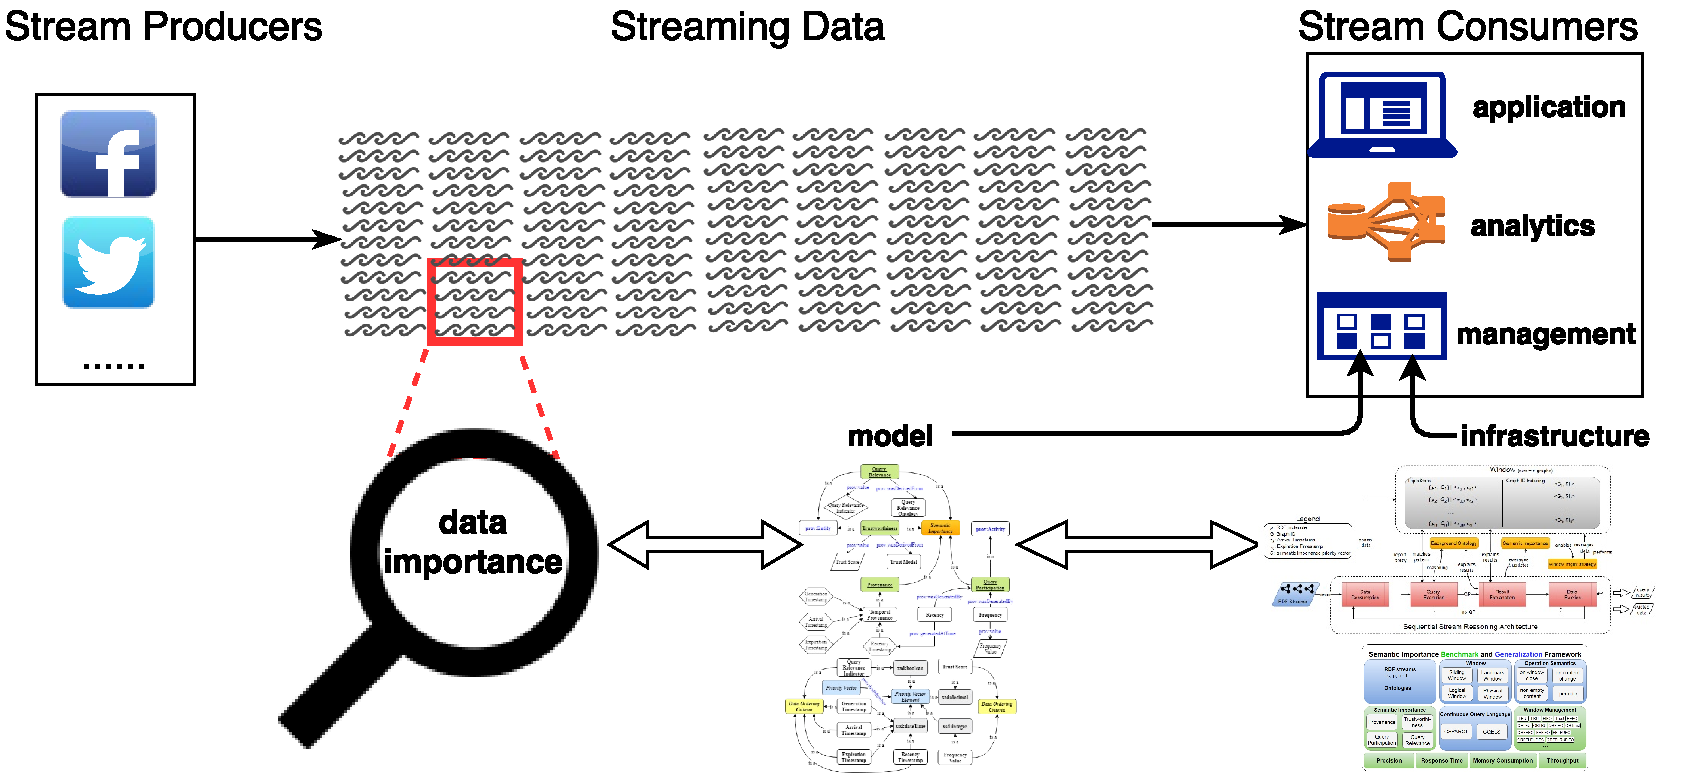
\includegraphics[width=5in]{img/1-tv.pdf}
    \caption{Dissertation Vision}
    \label{fig:1-tv}
\end{figure}

Streaming data is boundless, enormous, and frequently updated \cite{rodriguez2009semantic}.
It usually has intrinsic orders. 
For example, when a sequence of streaming data items arrive at the system, they are stamped with arrival timestamps.
This arrival ordering is only scratching the surface, because there are many other data orderings. 
Data can be ordered by when it is expired, where it comes from, how much it can be trusted, how precise it is, how relevant it is to the query, etc \cite{della2013order}. 

Stream reasoning, defined as ``logical reasoning in real time on gigantic and inevitably noisy data streams in order to support decision process of extremely large number of concurrent users'' \cite{barbieri2010stream}, is a newly identified research area that aims to bridge semantic reasoning with stream processing, so as to extract hidden information out of the streams.
Stream reasoning processes RDF streams \cite{barbieri2010querying}, defined as ``an infinite ordered sequence of data items'' \cite{srtutorial}, that model data streams by extending RDF.
The data items in RDF streams can be either triples or graphs, annotated by time-point timestamps or time-interval timestamps.

Stream reasoning has two key notions \cite{barbieri2010stream}, the sliding window \cite{arasu2003stream} and continuous processing \cite{babu2001continuous}.
A sliding window, or more generally a window, is a finite subset of the data stream, and manages the data.
Continuous processing repeatedly evaluates the data in the window as the window proceeds. 
The sliding window has two parameters, a size and a step \cite{stuckenschmidt2010towards}.
The size indicates how much data an active window can hold.
The step describes how far a window can move at one time.
According to the defined sliding window semantics \cite{botan2010secret}, a sliding window's size and step should be both fixed over the same stream. 

Windows have different types \cite{barbieri2010querying}:
a logical or temporal window has its step and size defined in the time domain; 
a physical or tuple window has a tuple-based step and size.
Windows can also be categorized based on the relationship between the size ($l$) and step ($d$):
if $d < l$, it is a sliding window;
if $d = l$, it is a tumbling window;
if $d > l$, it is a sampling window \cite{calbimonte2010enabling}. 
The behavior of a window is modeled by window operational semantics \cite{botan2010secret}, \cite{dell2013correctness}. 
It includes four aspects: scope, content, report and tick. 
Scope not only determines the boundary of an active window, but also affects the starting time ($t_{0}$) of the continuous processing.
Content describes the subset of the data stream that is currently in an active window.
Report defines the condition to fire the query.
Common policies include ``on content change'', ``on window full'', ``non-empty content'' and ``periodic''.
Tick defines how and when to react to the input, which can be either tuple-driven or time-driven.  
%
\section{The Silent Temporal Assumption}

\begin{figure}[!htbp]
	\centering
    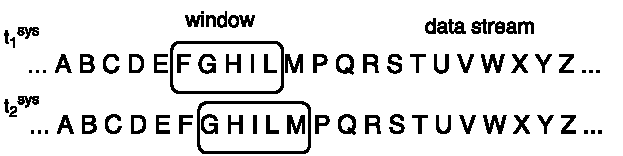
\includegraphics[width=5in]{img/1-sta.pdf}
    \caption{The Silent Temporal Assumption}
    \label{fig:1-sta}
\end{figure}

Figure \ref{fig:1-sta} shows a data stream being processed by two windows at $t^{sys}_1$ and $t^{sys}_2$ time respectively. 
Data is processed under a popular window management strategy called first in first out (FIFO), such that the window will have to evict the oldest data item A in order to consume the latest data item B at $t^{sys}_{2}$.
FIFO is based on the \textbf{silent temporal assumption} that ``older information becomes irrelevant at some point'' \cite{barbieri2010stream}, \cite{stuckenschmidt2010towards}.
A lot of stream reasoning work is based on this assumption.
For example, 
``... new items are often more accurate and relevant than older items ...'' \cite{golab2003processing};
``... recent items are typically more relevant than older ones ...'' \cite{barbieri2010deductive}.

FIFO is computationally efficient, but ultimately problematic depending on the window size and streaming data characteristics. 
This dissertation will show the problems related to the silent temporal assumption, as well as the approaches to solve the problems by loosening this assumption. 
%
\section{A Running Example}
In general, not all of the data items in streams can be used to answer the query \cite{mileo2013streamrule}.
There are situations where a single data item contains sufficient information (Situation 1), or multiple data items are required (Situation 2), so as to provide query answers. 
For the sake of convenience, this dissertation uses a term called \textbf{necessary data item} to refer to the data items that contain necessary information for question answering. 

The FIFO window management strategy based on the silent temporal assumption can work well in Situation 1. 
For Situation 2, the answer will only be returned when all of the necessary data items exist in the window at one time-point. 
However, the distance among necessary data items can be arbitrarily apart, and if this distance is longer than the window size, false answers will be generated. 
In order to illustrate this problem, this dissertation uses a running example of real-life soccer offside offence detection.

\begin{figure}[!htbp]
	\centering
	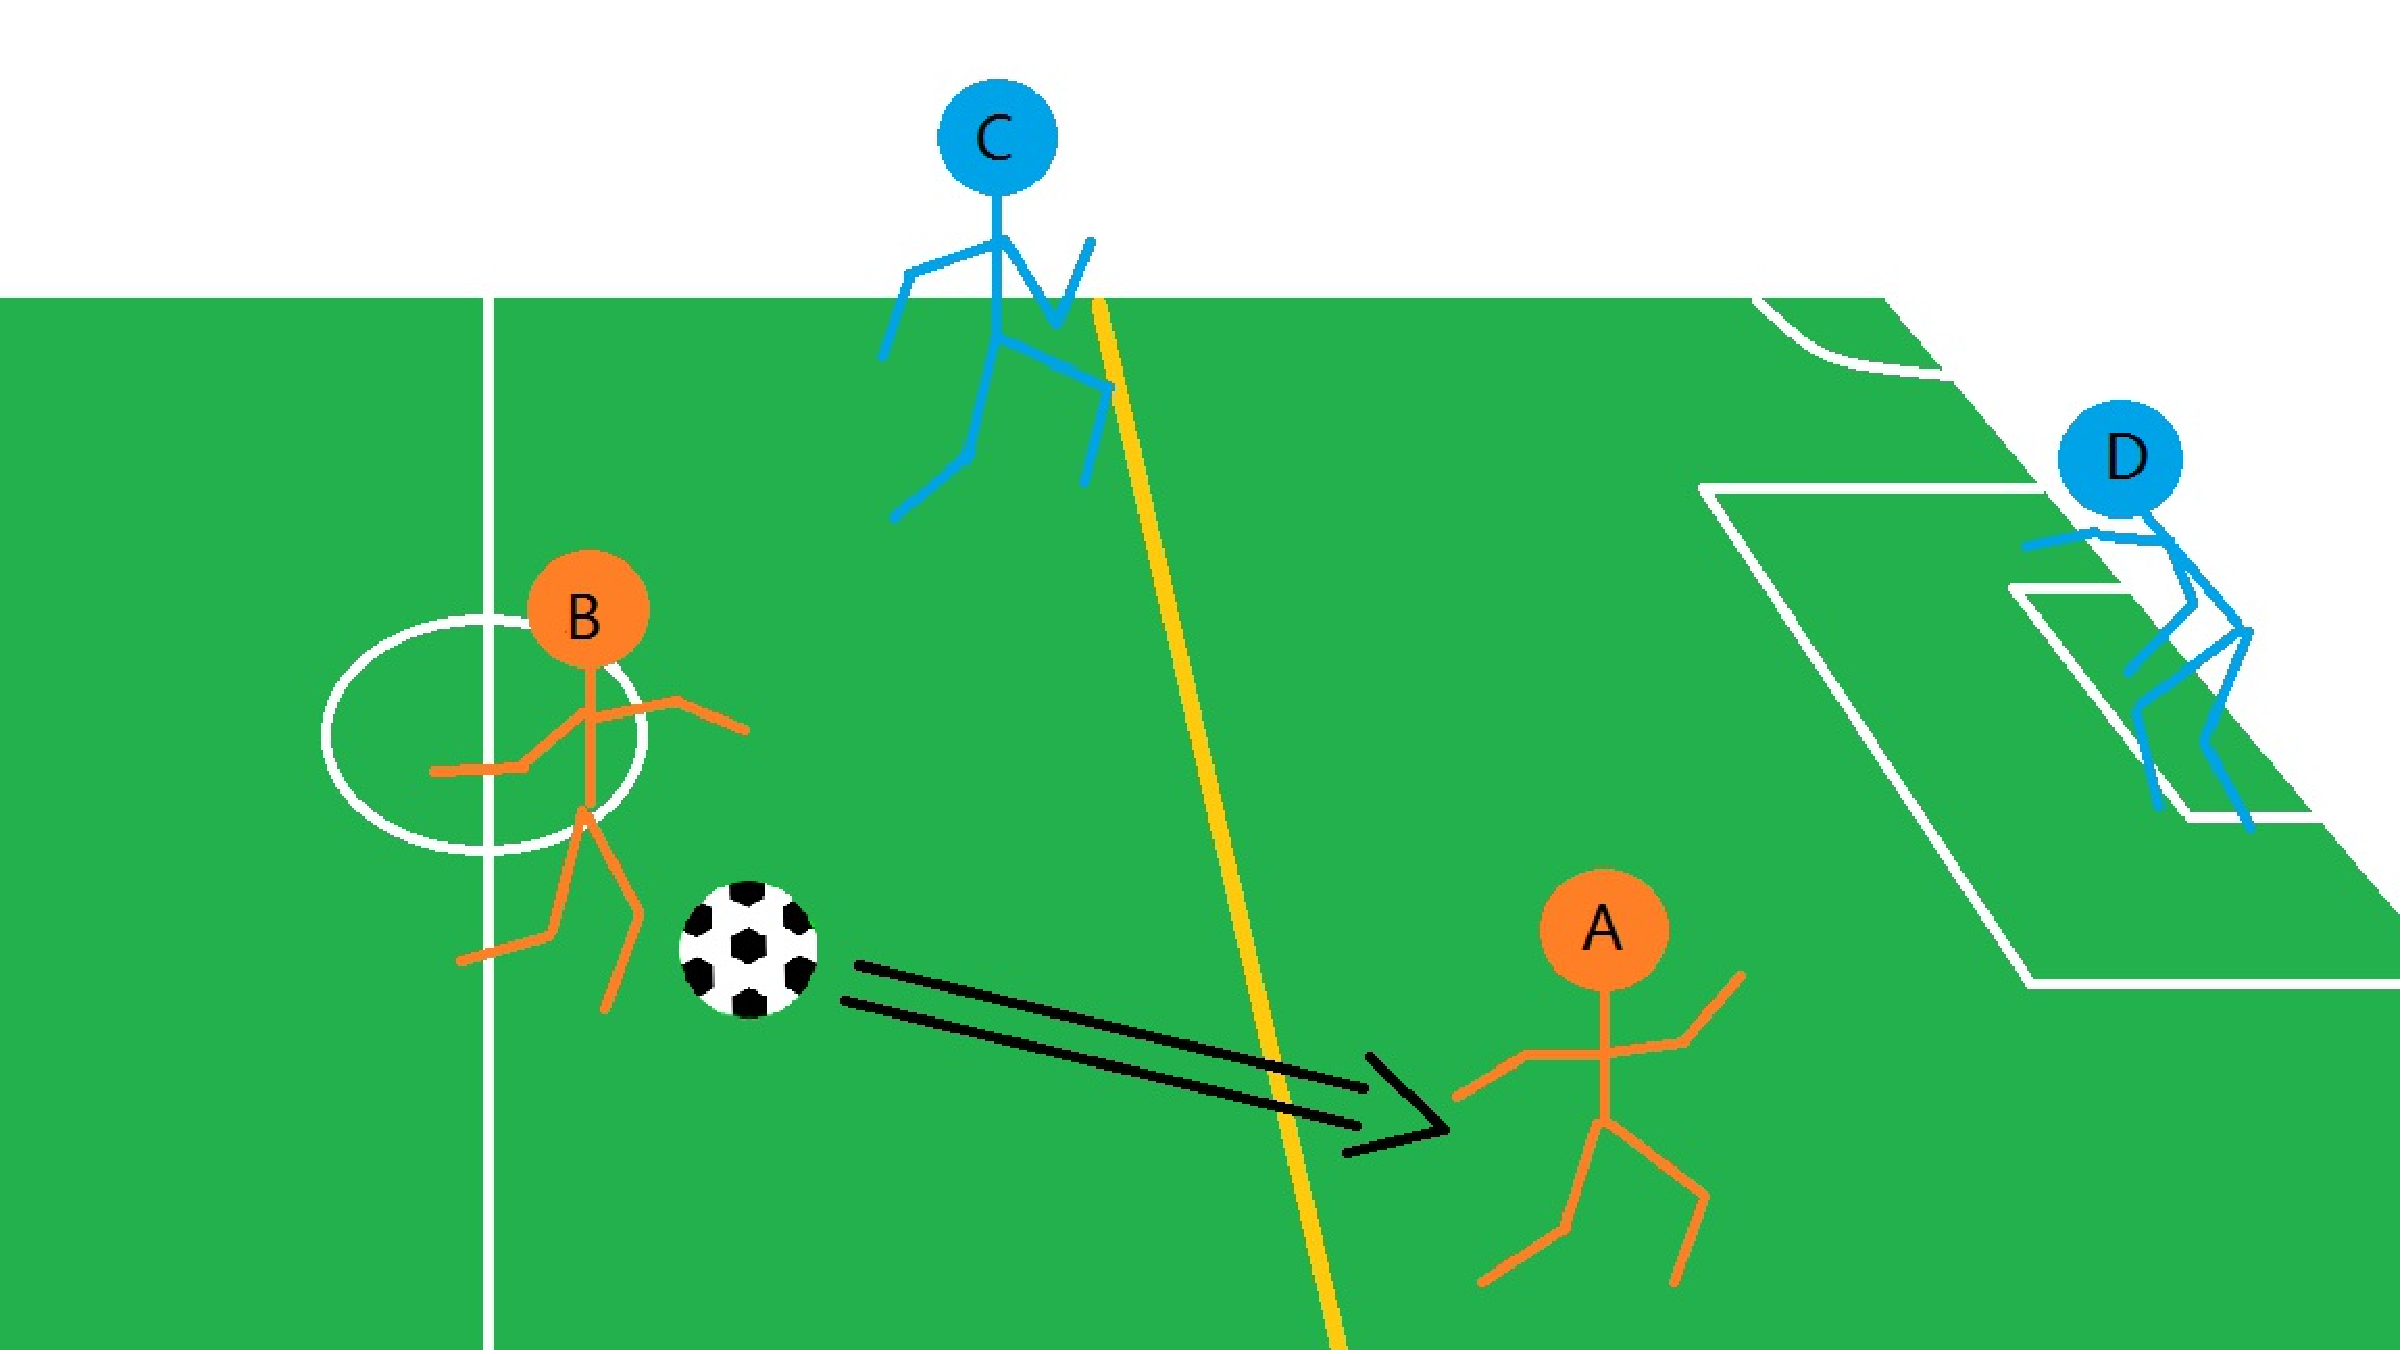
\includegraphics[width=5in]{img/1-soe.pdf}
	\caption{A Soccer Offside Example}
	\label{fig:1-soe} 
\end{figure}

Soccer offside offence is a common offence, which easily decides the direction where the game goes, thus can be very controversial sometimes.
F\'ed\'eration Internationale de Football Association (FIFA) defines soccer offside offence in a comprehensive way \cite{federation2016laws}. 
In this dissertation, a simplified definition will be used: 
a soccer offside offence is committed if an attacker who is at an offside position involves in an active play. 
So there are three atomic data items needed in order to determine an offside offence:
an attacker who is a member of a team that controls the ball;
this attacker is at an offside position that is nearer to the opponent's goal line than both the second last defender and the ball;
and this attacker involves in an active play, meaning that he/she either touches the ball or challenges an opponent. 
Figure \ref{fig:1-soe} shows a soccer offside offence example, where Player A and B are attacking.
Player A is at an offside position indicated by the yellow line. 
The moment that Player A becomes the first person to touch the ball passed from B is when an offside offence is committed.

Reasons to use this running example are two-folds.
First, situations in a soccer game can change all the time, thus a soccer offside offence can happen anytime in a very fast period. 
Second, the three atomic data items to determine a soccer offside offence will not arrive at the same time. 
This is because time will elapse as the ball is passed from Player B to Player A, and some other data will be generated during that time, such as players' positional data.

\begin{table}[!htbp]
	\centering
	\caption{Soccer Streaming Data Items}
	\label{tab:icons}
	\begin{tabular}{|c||c|c|c|} \hline
		icon & annotation & example & data sample \\ \hhline{|=#=|=|=|}
    	$\times$ & position & \makecell{$\times_{A}$ \\ $\times^{\circ}_{A}$} & \makecell{:PlayerA :hasPosition :PositionA \\ :PlayerA :hasPosition :OffsideOffencePosition} \\ \hline 
		$\largecircle$ & \makecell{active play \\involvement} & $\largecircle_{A}$ & :PlayerA a :BallLastToucher \\ \hline
		$\largetriangleup$ & attacker & $\largetriangleup_{A}$ & :PlayerA a :Attacker \\ \hline
		$\largesquare$ & defender & $\largesquare_{A}$ & :PlayerA a :Defender \\ \hline
	\end{tabular}
\end{table}

The data stream used for the running example throughout this dissertation contains four different types of data items in Table \ref{tab:icons}.
$\times$ indicates a player's positional data;
$\times^{\circ}$ denotes the offside position of a player; 
$\largetriangleup$ refers to an attacker;
$\largesquare$ describes a defender;
$\largecircle$ represents that some player involves in an active play, such as touching the ball, challenging an opponent, etc.

Together with these denotations, and the logic and-operator ($\wedge$), that Player A commits an offside offence can be expressed as
$\largetriangleup_{A} \wedge \times^{\circ}_{A} \wedge \largecircle_{A}$. 
Players on the field move from time to time, which will make offensive transitions happen at any moment.
Any player can involve in an active play. 
Thus these four kinds of the data items can form a data stream that reflects the situations on the field.
This example also assumes that a stream reasoning application consumes this data stream and constantly looks for players who commit offside offences. 
%
\section{Early Eviction}

\begin{figure}[!htbp]
	\centering
	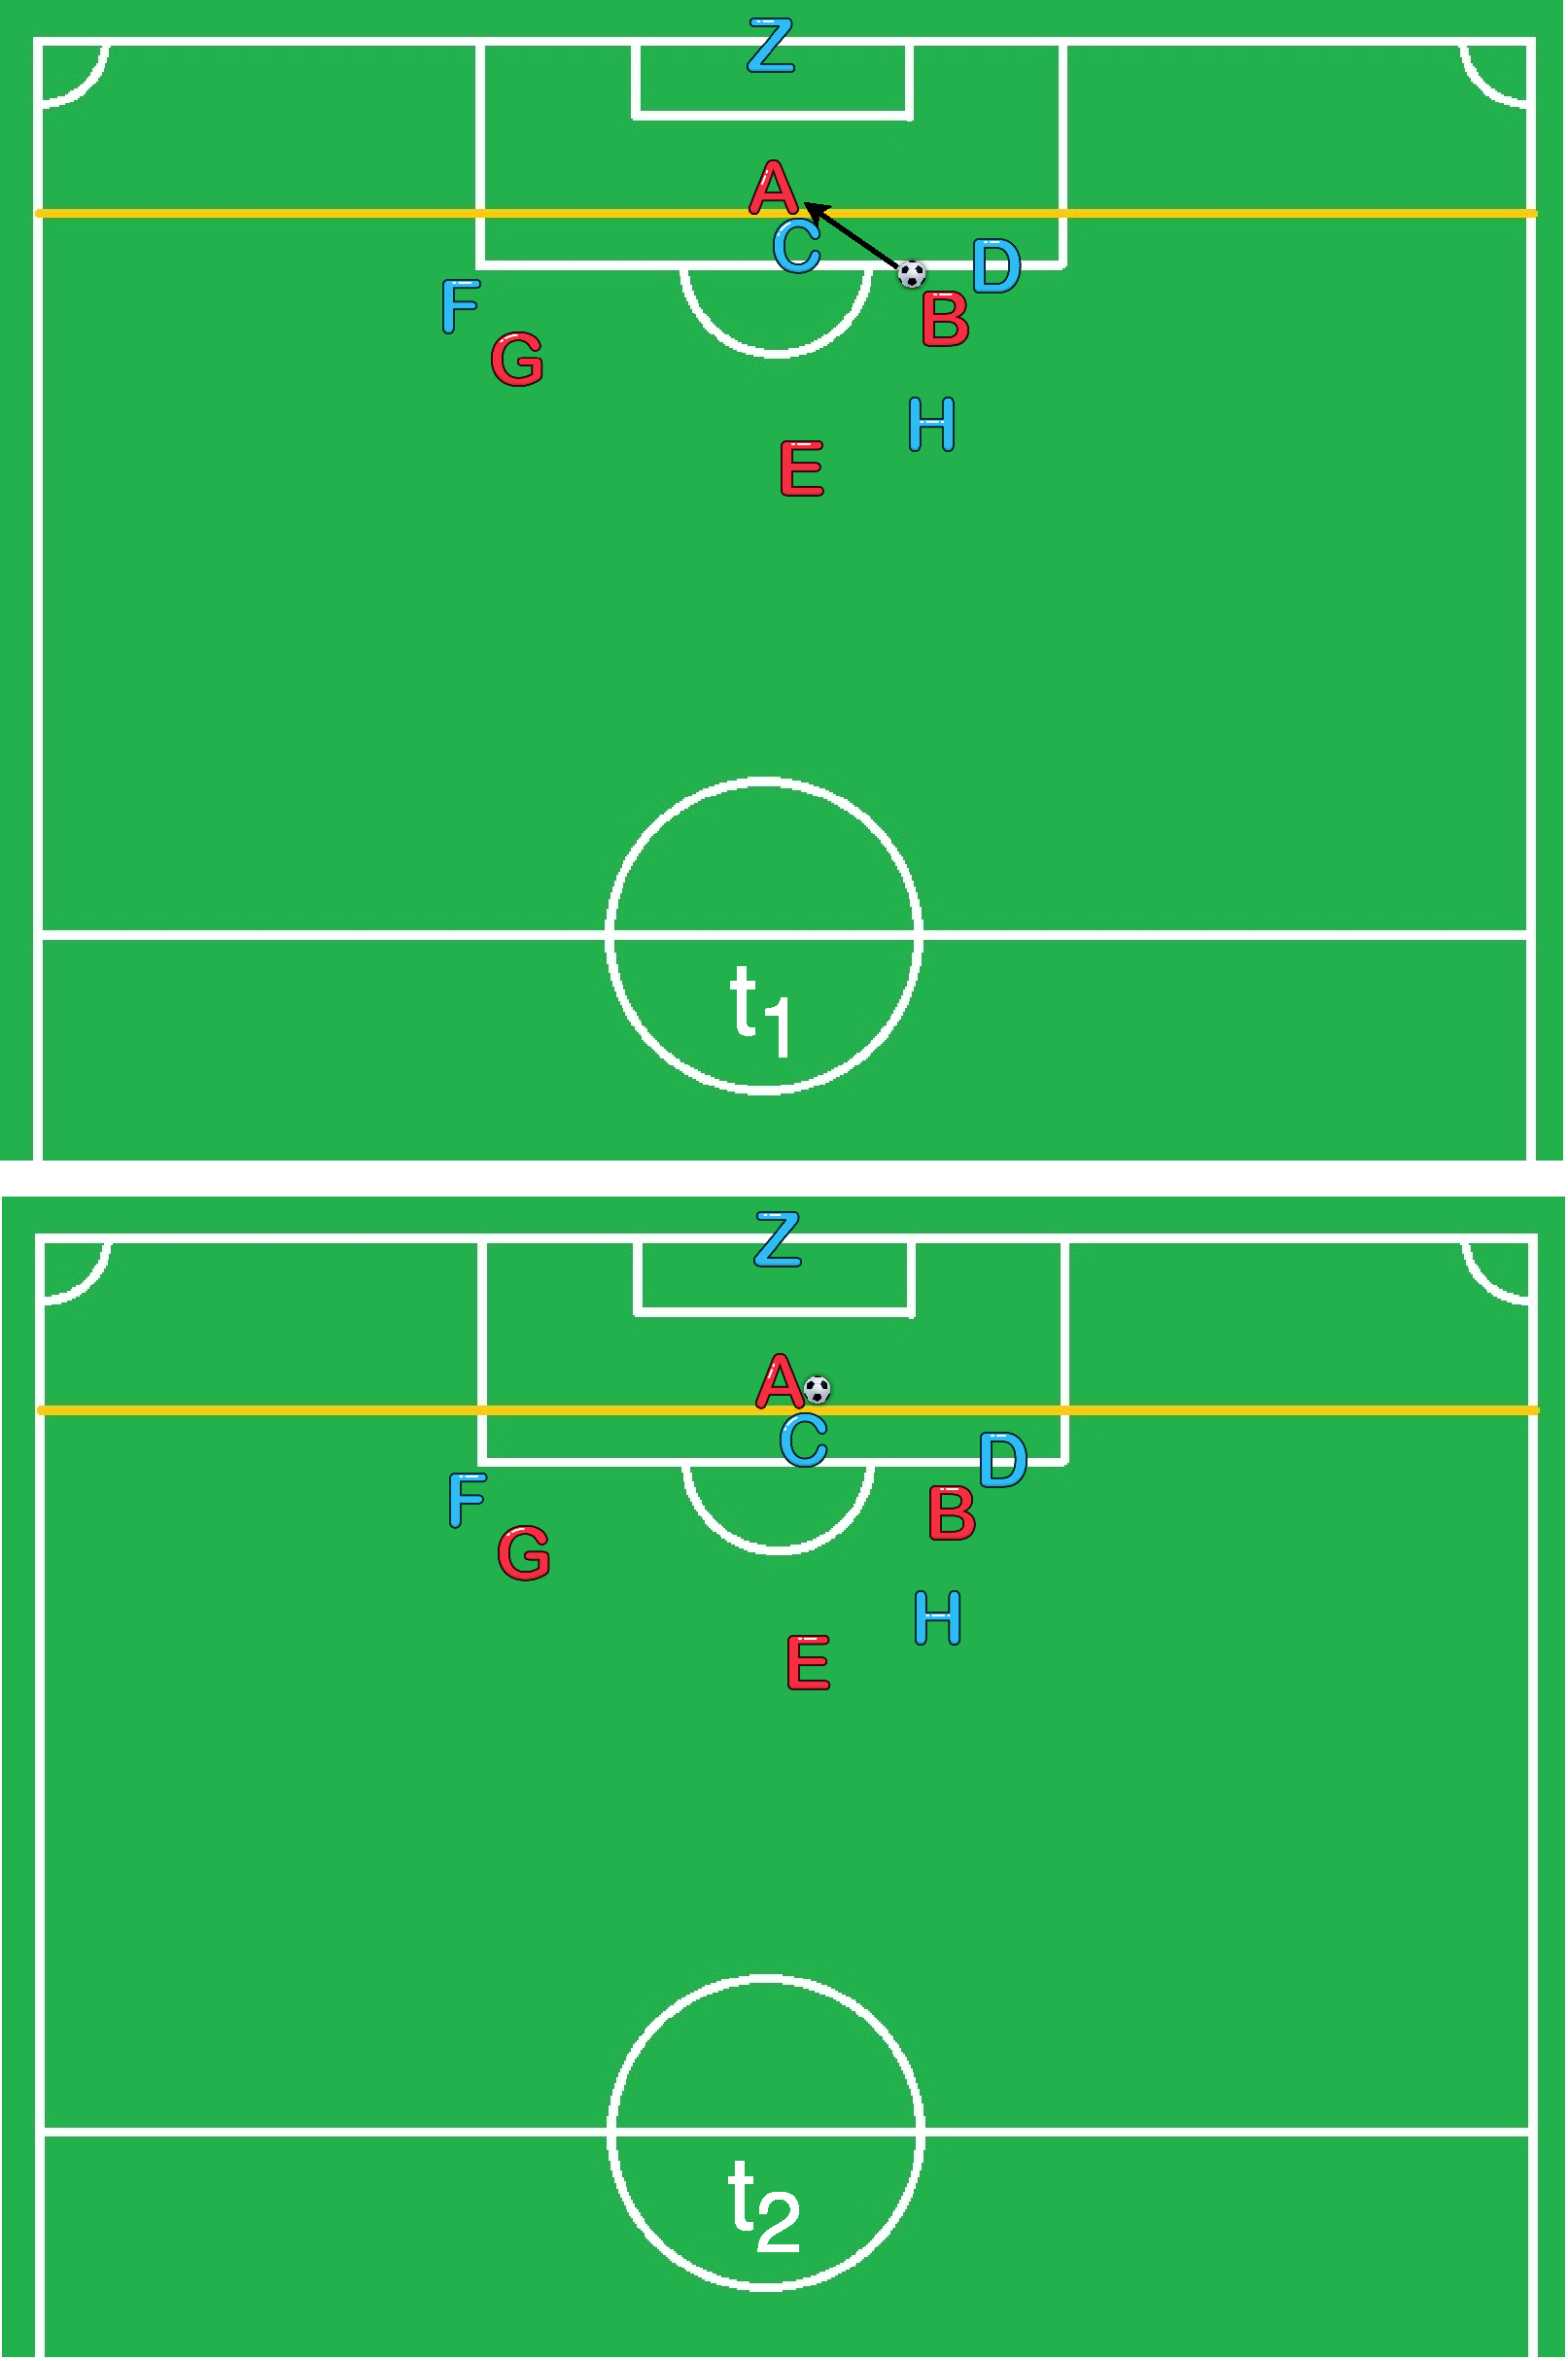
\includegraphics[width=5in]{img/1-seeh.pdf}
	\caption{Soccer Offside Early Eviction}
	\label{fig:1-seeh} 
\end{figure}

Consider the situation in Figure \ref{fig:1-seeh}:
at $t_{1}$ time, red team is attacking.
Player B is passing the ball to Player A who is at an offside position indicated by the yellow line. 
At $t_{2}$ time, Player A is the first one to get the ball and about to take a shot.
At this moment, the linesman flags to notify the referee that Player A commits an offside offence.\footnote{Conventionally, a linesman usually flags if he/she thinks Player A will be the first one to touch the ball so as to help save some stamina.}

\begin{figure}[!htbp]
	\centering
	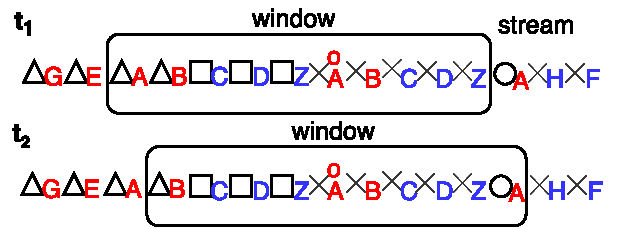
\includegraphics[width=5in]{img/1-seew.pdf}
	\caption{Early Eviction in Sliding Window with FIFO}
	\label{fig:1-seew} 
\end{figure}

Figure \ref{fig:1-seew} shows what is happening in the window. 
At $t_{1}$, $\largetriangleup_{A}$ and $\times^{\circ}_{A}$ are both in the window. 
$\largecircle_{A}$ is about to enter the window. 
However, in order to consume $\largecircle_{A}$, $\largetriangleup_{A}$ has to be evicted because of the silent temporal assumption. 
Thus at $t_{2}$, only $\times^{\circ}_{A}$ and $\largecircle_{A}$ exist in the window. 
In either time-point, there is no way to have all three of the necessary data items in the window, causing a false-negative answer. 
Namely, there should be an offside offence but the system fails to detect it. 
This problem is called \textbf{early eviction}: necessary data items are evicted too early before they can be used to answer queries. 

There is a naive solution to the early eviction problem: 
to increase the window size such that it can hold $\largetriangleup_{A}$, $\times^{\circ}_{A}$, and $\largecircle_{A}$ in the same active window.
Nonetheless, increasing the window size will possibly result in having more data within one window, which can drain more system memory and computation resources. 
Increasing window size based on the exact distance among all necessary data items is also not feasible, as in general data items can be arbitrarily apart, and one cannot foretell these distances.
%
\section{Early Expiration}

\begin{figure}[!htbp]
	\centering
	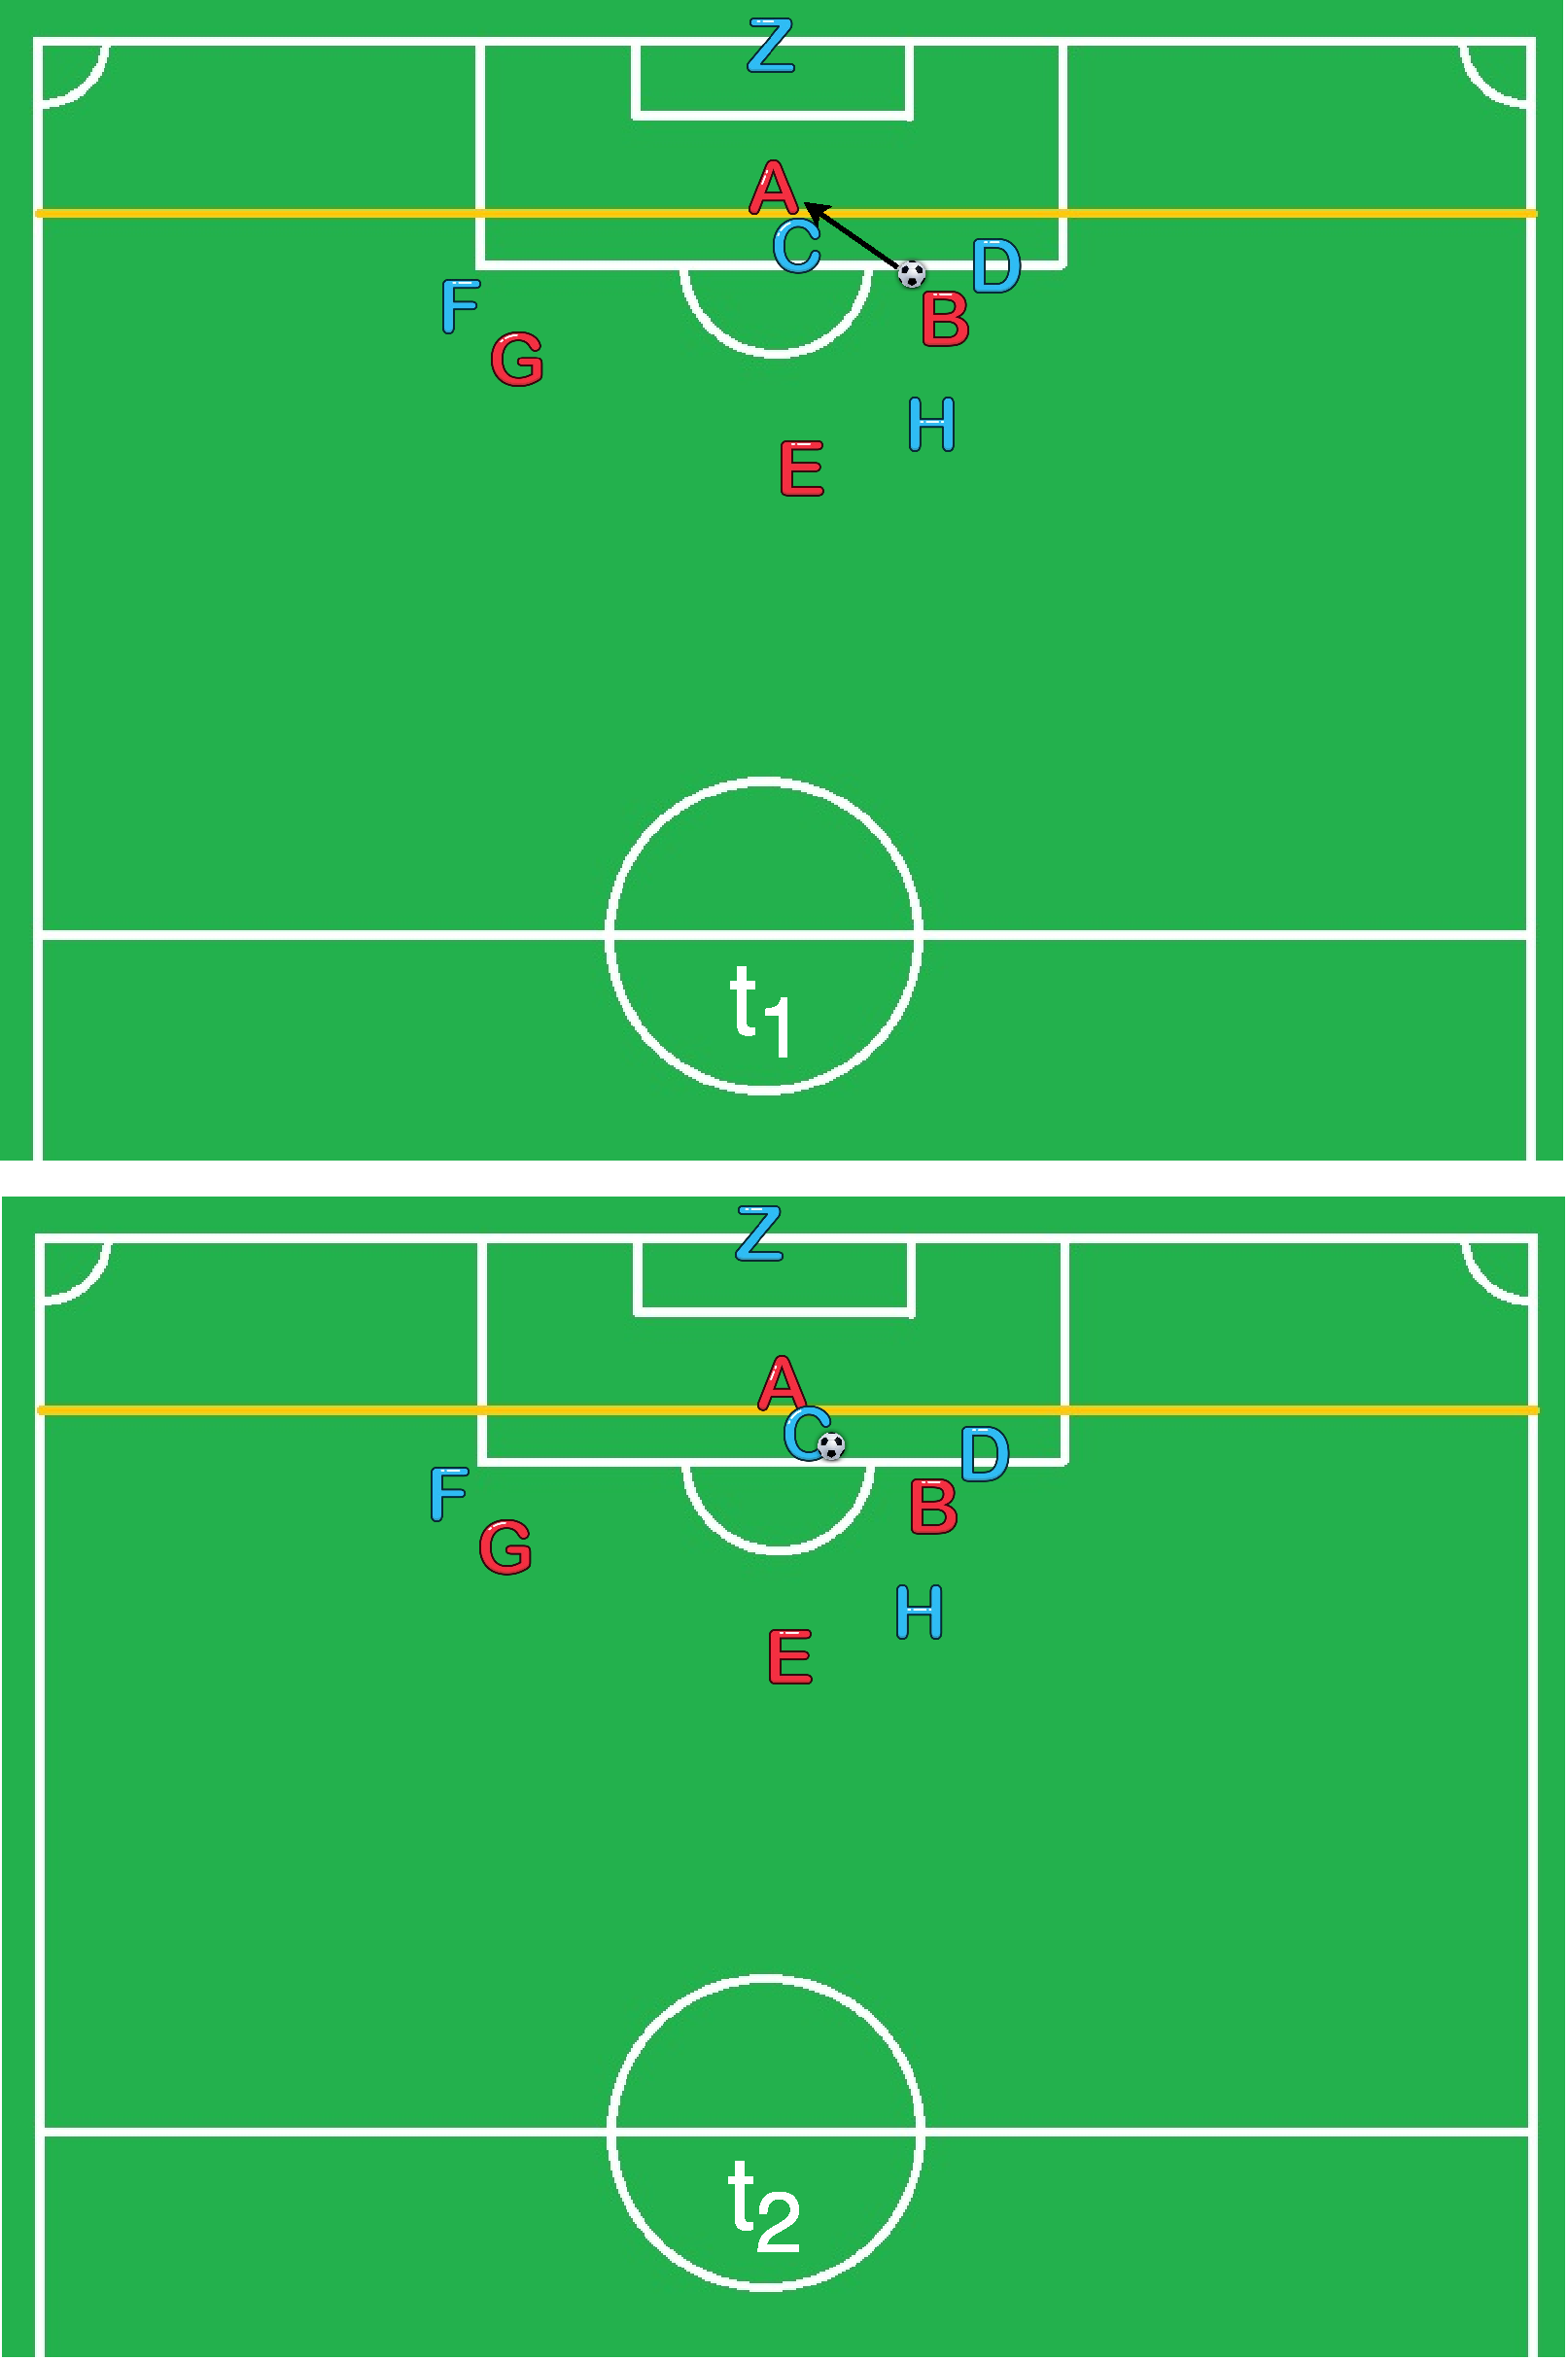
\includegraphics[width=5in]{img/1-seex.pdf}
	\caption{Soccer Offside Early Expiration}
	\label{fig:1-seex} 
\end{figure}

Figure \ref{fig:1-seex} shows another possible situation during a soccer game. 
Again at $t_{1}$, red team is attacking, and Player B is passing the ball to Player A who is at the offside position.
During $t_{1}$ to $t_{2}$, what happens is that Player C successfully steals the ball.
Then Player A immediately challenges Player C in order to grab the ball back. 
At the moment when Player C steals the ball, there is an offensive transition going on.
The blue team is now controlling the ball, thus the red team becomes defensive. 
According to our simplified definition of soccer offside offence, a defender cannot commit an offside offence. 
Thus, the linesman doesn't take any action and let the match continue. 

\begin{figure}[!htbp]
	\centering
	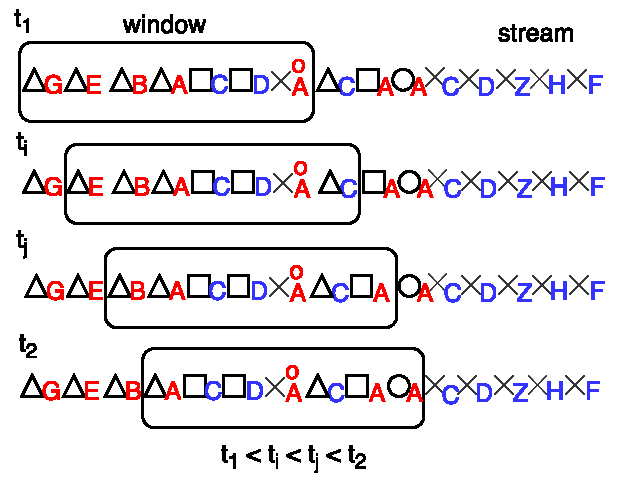
\includegraphics[width=5in]{img/1-seexw.pdf}
	\caption{Early Expiration in Sliding Window with FIFO}
	\label{fig:1-seexw} 
\end{figure}

Figure \ref{fig:1-seexw} shows how sliding window processes the soccer streaming data from Figure \ref{fig:1-seex}. 
As the sliding window moves, $\largetriangleup_{G}$ and $\largetriangleup_{E}$ are successively evicted to make room for $\largetriangleup_{C}$ and $\largesquare_{A}$.
At $t_{i}$, there is already a contradictory: to the window, Player C is both a defender and attacker. 
Although $\largetriangleup_{C}$ and $\largesquare_{C}$ carry different arrival or generation timestamps, these timestamps are only annotations.
For stream reasoning engines such as C-SPARQL \cite{barbieri2010execution}, the continuous query will be parsed into a SPARQL query that is totally blind about the timestamps. 
At $t_{j}$, there is a same contradictory for Player A who is both a defender and an attacker. 
As time reaches $t_{2}$, $\largecircle_{A}$ arrives. 
So all the necessary data items, $\largetriangleup_{A}$, $\times^{\circ}_{A}$, and $\largecircle_{A}$ are in the window, resulting a false-positive answer, i.e. there should not be an offside offence but the system reports positively. 
As a matter of fact, $\largetriangleup_{A}$ should be expired as $\largesquare_{A}$ arrives.
Because there is a transition already happened, the role of Player A is changed from attacker to defender. 
However, due to the silent temporal assumption, the FIFO strategy will not evict $\largetriangleup_{A}$ until after $t_{2}$.
This problem is called \textbf{early expiration}: the data item expires within the window, potentially causing inconsistency or leading to a wrong query answer depending on whether this data item is necessary to answer the query. 
%
\section{Research Hypotheses}
This dissertation is built upon the research hypothesis (RH) that \textit{semantically driven data orderings can effectively capture the data importance. By leveraging data importance modeled from various streaming data orderings, a window in the stream reasoning system can manage data in a smart and flexible way, by which the system precision, response time, memory consumption and throughput can be improved.}
This hypothesis can be represented as a diagram shown in Figure \ref{fig:1-rh}.
Specifically, this hypothesis can be decomposed into following four sub-hypotheses:

\begin{figure}[!htbp]
	\centering
	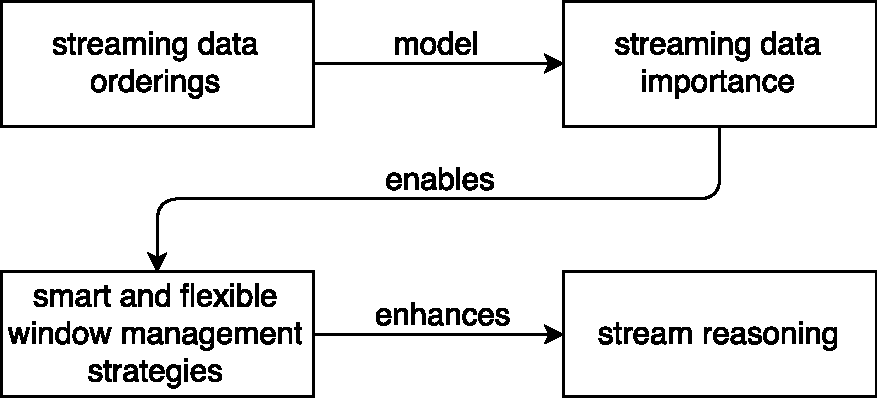
\includegraphics[width=5in]{img/1-rh.pdf}
	\caption{Research Hypothesis}
	\label{fig:1-rh} 
\end{figure}

\textbf{RH1:} \textit{data orderings can model data importance.}
Semantic importance is stated by observing the fact that streaming data usually has intrinsic orderings \cite{della2013order}. 
This not only includes temporal orderings such as arrival/expiration timestamps, but also precision ordering, trust ordering, geo-location ordering, relevance ordering, etc. 
This dissertation hypothesizes that all of these data orderings can be leveraged to model the data importance. 
For example, a data item can be important if it arrives later, or has a bigger trust score, or both. 

\textbf{RH2:} \textit{data importance can enable window management strategies.}
The model of data importance can be used as the window management strategies, which control how window consume, manipulate, query and evict the data.
FIFO is a common strategy under the silent temporal assumption. 
A semantic importance enabled window management strategy possesses the ability to discriminate the data based on its importance. 
Consider if the data itself carries expiration timestamps, the window should pay attention to the data expiration within the window to guarantee valid results.
In this setting, ``not expired'' should be seen as more important. 
An expiration-priority window consumes the most recent data, then evicts all the expired data, then executes the query on it. 
It should also take care of the data expiration during the query execution process. 

\textbf{RH3:} \textit{window management strategies can improve stream reasoning system performance.}
Stream reasoning systems are born with the time constraints, which hinders real-time and correct outputs.
A smaller-sized window holds less data to process, and possibly faster response time, but can potentially provide worse results due to being incapable to hold enough data, especially under the FIFO strategy.
However, if the window can distinguish the right data that can contribute to the query results according to the data importance, the window size can be set to only hold that amount of necessary data. 
In this way, less but enough data for correct results needs to be stored, less computations need to be executed, and more response time is saved, thus the system is able to process more data items within a unit time. 

\textbf{RH4:} \textit{different window management strategies can produce different results.}
Window management strategies are different, which causes the data in the window to be different, even for the same stream. 
The query will be executed on this data, thus the results will be different. 
This hypothesis emphasizes the suitability between the use case requirements and the window management strategies. 
It is critical to deploy suitable strategies in different use cases to maximize the benefits.
%
\section{Research Goal}

\begin{figure}[!htbp]
	\centering
    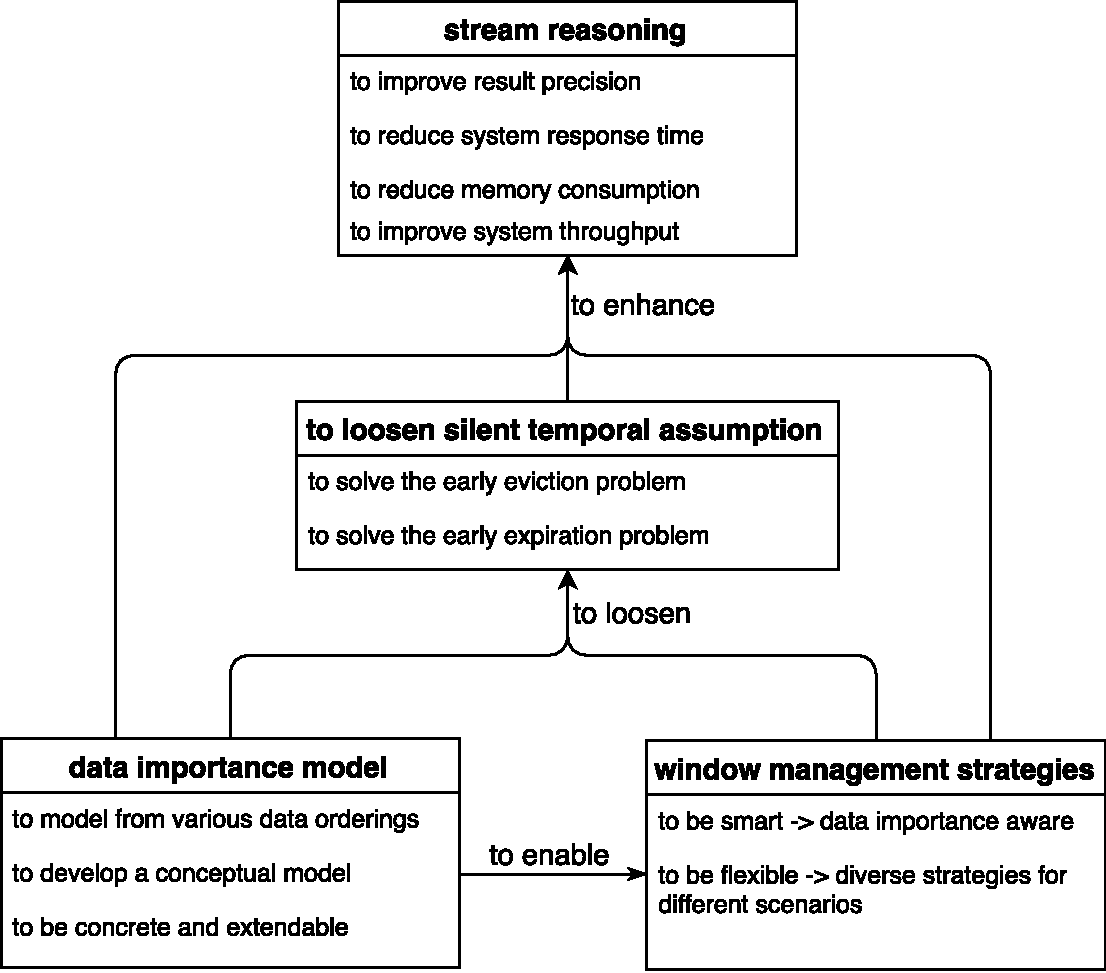
\includegraphics[width=5in]{img/1-rg.pdf}
    \caption{Research Goal}
    \label{fig:1-rg}
\end{figure}

This dissertation aims to achieve the goal in Figure \ref{fig:1-rg}.
This dissertation targets to enhance stream reasoning by loosening the silent assumption via explicitly modeling the importance of the streaming data to the query at hand.
In order to do so, the dissertation will first propose a data importance model developed from various streaming data orderings. 
With this data importance model, smarter and more flexible window management strategies will be enabled. 
The silent temporal assumption can then be loosened by both the model and strategies.
Together with the loosened silent temporal assumption, the data importance model and window management strategies, stream reasoning can be enhanced. 

Specifically, this work will enhance stream reasoning from four perspectives: to improve system precision, to reduce response time, to reduce memory consumption, and to improve system throughput. 
``By loosening the silent assumption'' refers to solving the early eviction and early expiration problems. 
In order to explicitly model the streaming data importance, this dissertation proposes a concrete and expendable semantic conceptual model of data importance and enables smart and flexible window management. 
%
\section{Research Questions}

\begin{figure}[!htbp]
	\centering
	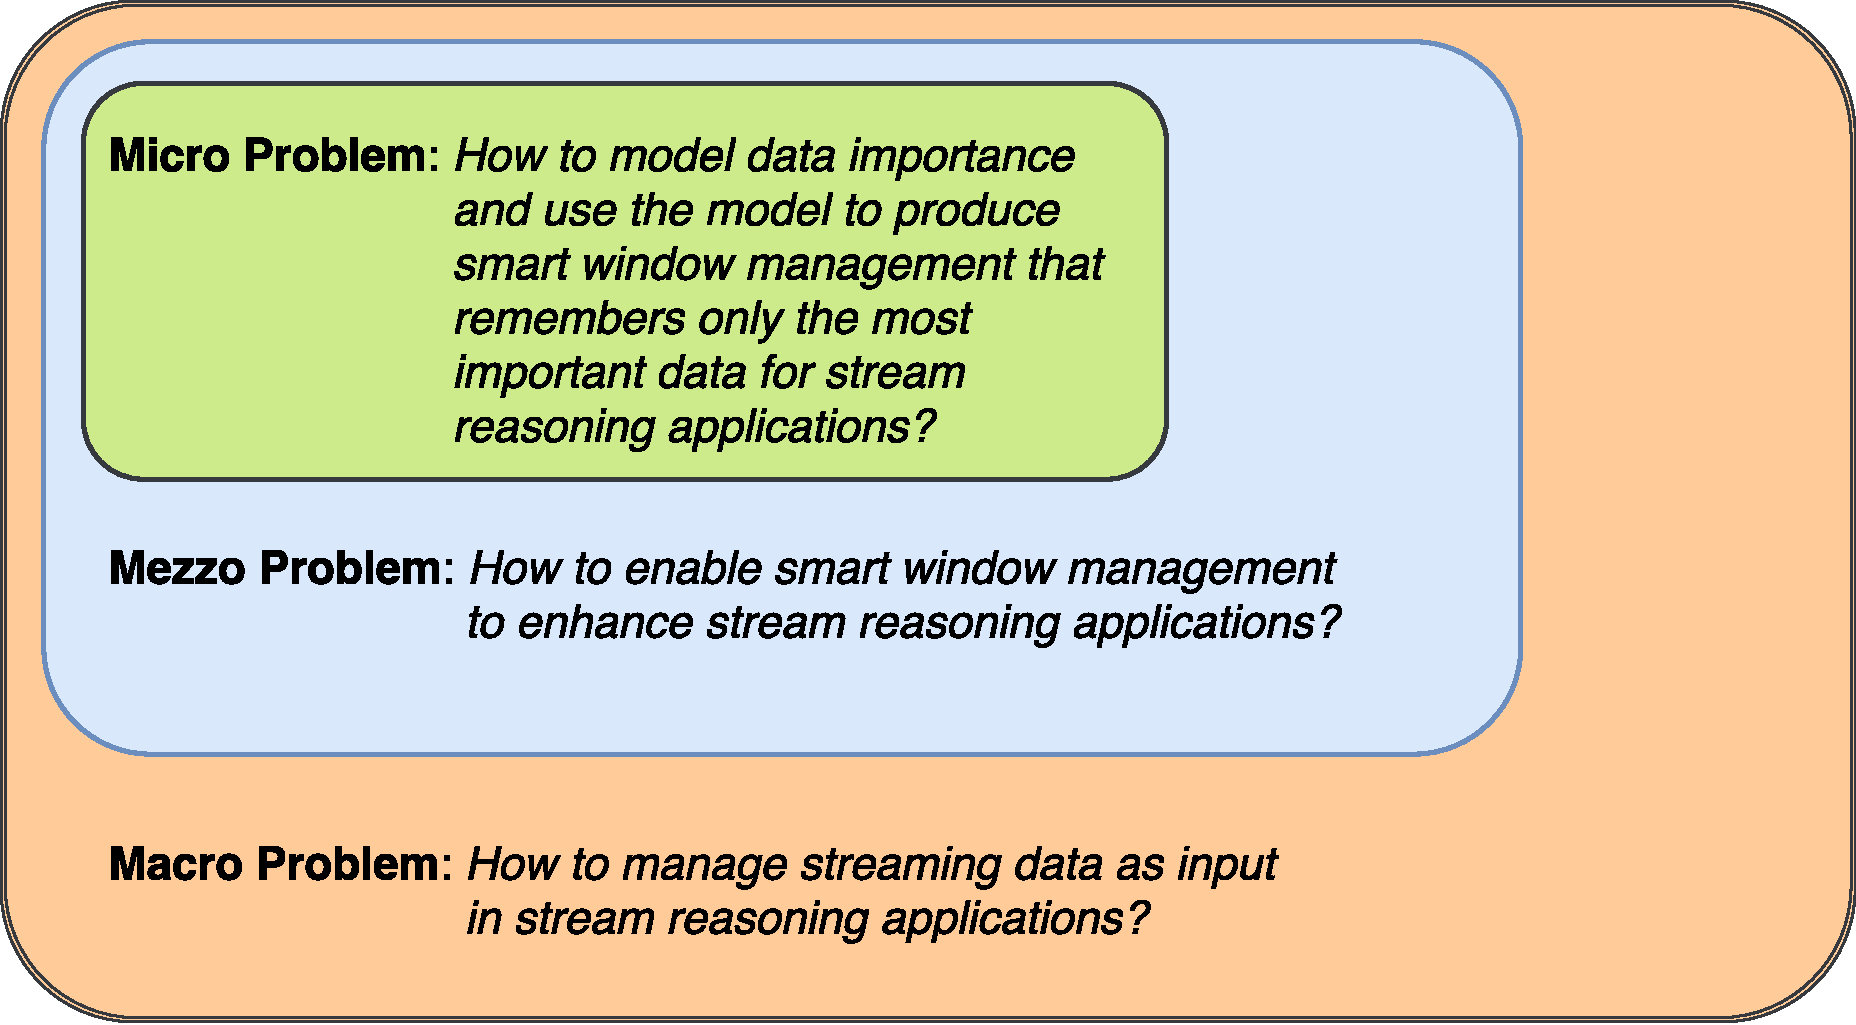
\includegraphics[width=5in]{img/1-rq.pdf}
	\caption{Research Questions}
	\label{fig:1-rq} 
\end{figure}

In general, this dissertation targets on streaming data management for stream reasoning. 
As mentioned in previous sections, the silent temporal assumption and FIFO management strategy are neither adequate to deal with problems of early eviction and early expiration. 
After all, these two problems influence the performance of the stream reasoning systems. 
So, a more concrete question is how to enable windows to manage streaming data in a both smart and efficient way, such that the stream reasoning systems can be enhanced. 
In order to answer this question, this work needs to define what a smart window management refers to, then how to enable this smart management. 
Figure \ref{fig:1-rq} displays the three research questions in a micro-mezzo-macro \cite{lacasse2015making} fashion.

The micro problem itself has defined what a smart window management is: to remember only the most important data. 
In order to enable this smartness, the system has to know what the data importance is about, and how to rank the data based on its importance. 
Thus the problem boils down to model data importance that can be used during window managing streaming data. 

The mezzo problem is a level more general than the micro problem.
What it asks for is that if there is a solution for the micro problem, how to use this solution to enhance stream reasoning applications, and how to prove that this solution is general in a way such that it can be adapted into different scenarios and use cases. 
The window should know which data is more important than others. 
By only keeping the important data, window size can be shrank while the ability to answer the query is not influenced.
Keeping a smaller window size means smaller amount of data, which saves memory and reduces query execution time. 

The macro problem is how to manage the torrent, heterogeneous and large-scale streaming data for processing and reasoning. 
This problem is about the general vision of stream reasoning, including aspects of data model, query model, window operator, data processing etc, thus can be used to provide future research directions of this dissertation.  
%
\section{Dissertation Contributions}

\begin{figure}[!htbp]
	\centering
    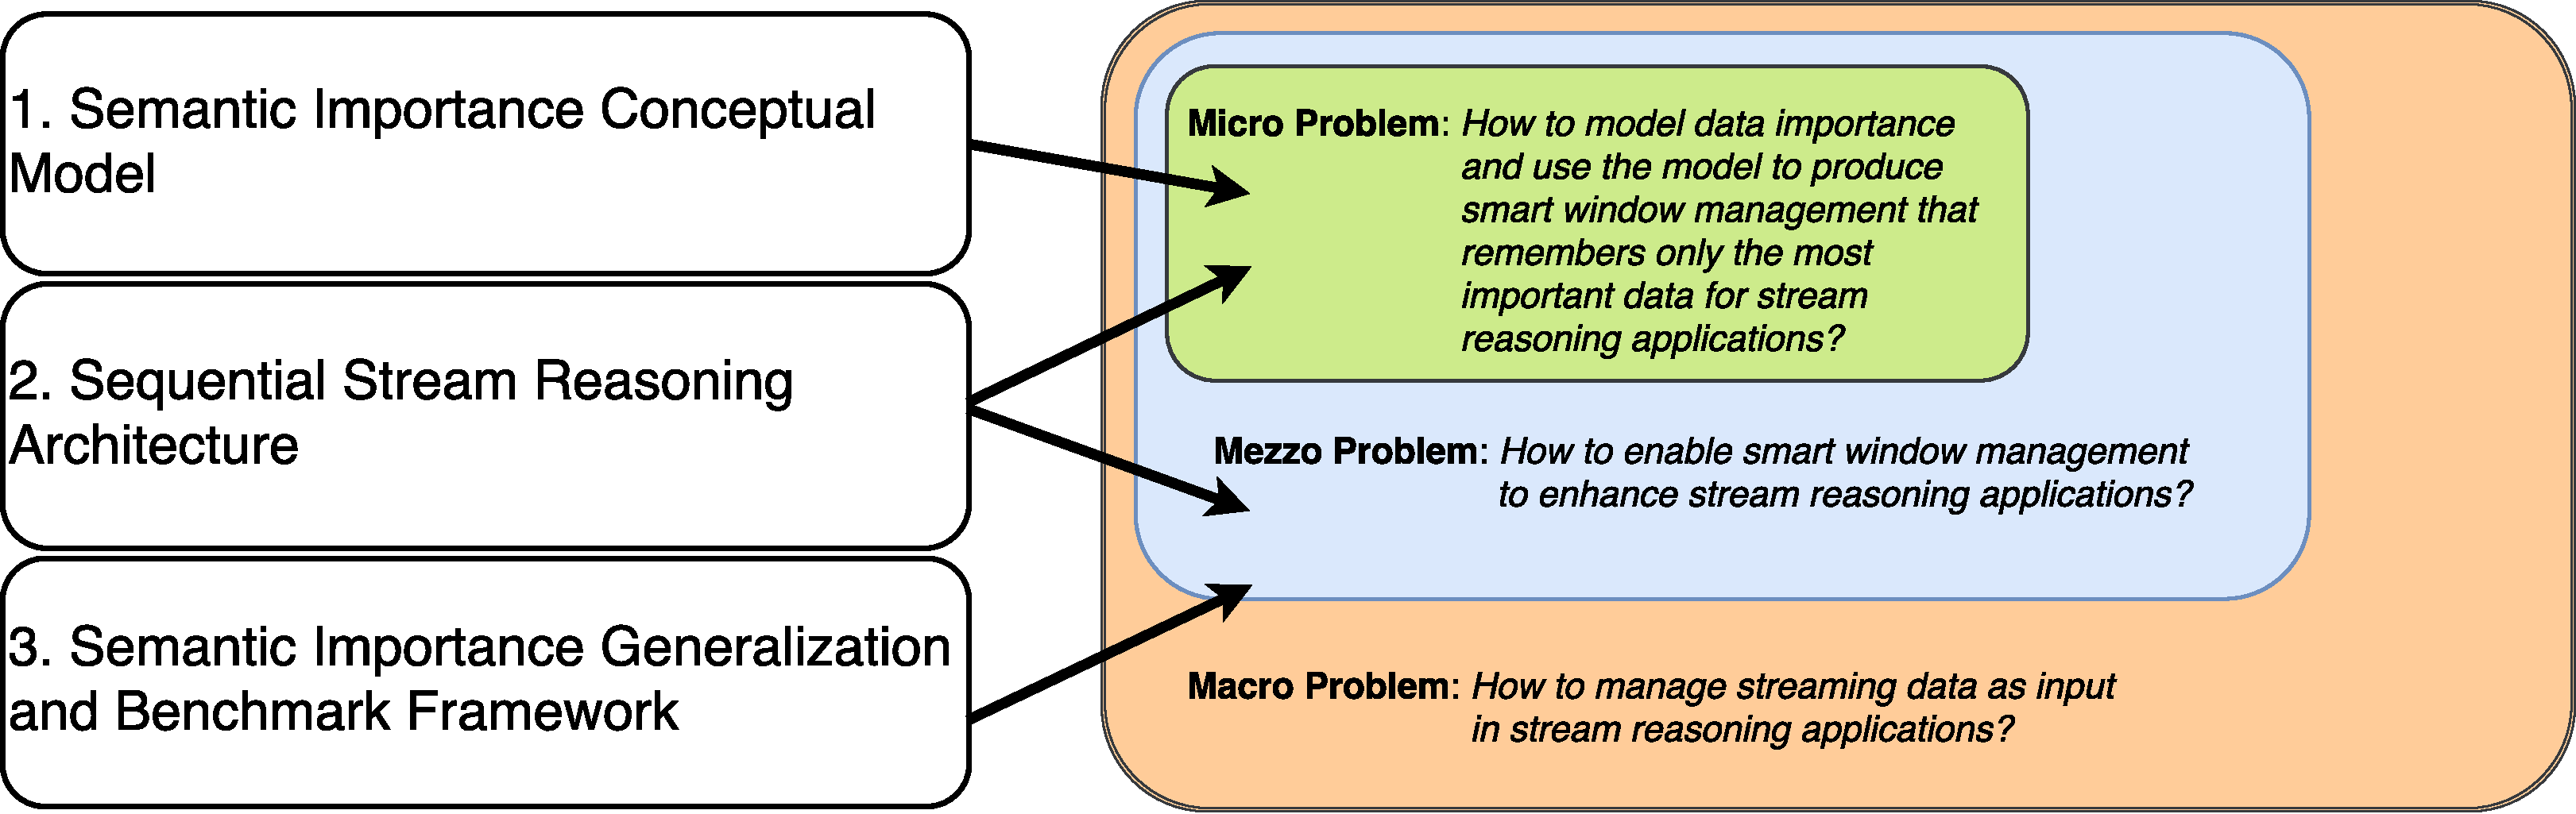
\includegraphics[width=5in]{img/1-dc.pdf}
    \caption{Dissertation Contributions}
    \label{fig:1-dc}
\end{figure}

This dissertation claims three contributions.
Figure \ref{fig:1-dc} shows each of them and how they can be mapped to help answer the research questions.

\textbf{Semantic Importance Conceptual Model}
The notion of ``semantic importance'' is proposed to describe the data importance from various streaming data orderings. 
Semantic importance currently includes four aspects,``provenance'', ``query participation'', ``trustworthiness'', and ``query relevance''.
These four aspects provide a preliminary set of metrics according to which different order-aware window management strategies can be constructed.
Each data item is associated with a semantic importance indicator that is embodied as a mathematical priority vector.
Priority vectors are comparable thus data can be ranked.
With this ranking, more important data can be preserved while less important data will be evicted, no matter how different orderings are chosen as semantic importance to be deployed in the system.

\textbf{Sequential Stream Reasoning Architecture}
Semantic importance is a new concept.
Most existing stream reasoning applications are not compatible with semantic importance.
However, in order to show how to deploy it and how many benefits it can bring, the sequential stream reasoning architecture has been designed and implemented.
This architecture has one window design, and four components arranged in a sequential work-flow: 
(1) a data consumption component that consumes streaming data and sends it to the streaming window;
(2) a query execution component that evaluates a standard SPARQL query against the data in the triplestore and background ontology; 
(3) a result explanation component that uses the query and reasoning process to explain how the result is generated;
(4) a data eviction component that evicts selected data from the window and then returns to the data consumption component for continuous processing.  
All the four sequential components are interacting with the window from time to time.
Leveraging this architecture and semantic importance, two use cases were implemented from different domains. 
The first use case explores soccer offside detection, where query contribution, provenance and query relevance are selected and evaluated. 
The second use case detects data exfiltration event in the insider threat domain, where trustworthiness and provenance are leveraged.
The results have shown that semantic importance is able to improve precision, response time, memory consumption, and throughput for stream reasoning.

\textbf{Semantic Importance Generalization and Benchmark Framework}
In order to provide the empirical support for the generalization of semantic importance, an evaluation framework is designed and implemented.
This framework generalizes semantic importance by connecting it with the state-of-the-art stream reasoning techniques, such as continuous query languages, window semantics, operational semantics etc. 
It also provides a comprehensive benchmark test bed, with various benchmark configuration parameters. 
It can work with either user provided data, or a default data generator that is evolved from LUBM data generator \cite{guo2005lubm}.
In this dissertation, the detailed experimental results are visualized and analyzed to illustrate the superiority of the semantic importance.
%%%%%%%%%%%%%%%%%%%%%%%%%%%%%%%%%%%%%%%%%%%%%%%%%%%%%%%%%%%%%%%%%%%% 
%                                                                 %
%                            CHAPTER Two                          %
%                                                                 %
%%%%%%%%%%%%%%%%%%%%%%%%%%%%%%%%%%%%%%%%%%%%%%%%%%%%%%%%%%%%%%%%%%% 

\chapter{RELATED WORK}
\blfootnote{* Portions of this chapter previously appeared as: Rui Yan, Mark T. Greaves, William P. Smith, Deborah L. McGuinness 2016. ``Remembering the Important Things: Semantic Importance in Stream Reasoning.'' Stream Reasoning 2016 Workshop, International Semantic Web Conference 2016. Rui Yan, Brenda Praggastis, William P. Smith, Deborah L. McGuinness 2016. ``Towards A Cache-Enabled, Order-Aware, Ontology-Based Stream Reasoning Framework.'' Linked Data on the Web Workshop 2016, International World Wide Web Conference 2016. Rui Yan, Brenda Praggastis, William P. Smith, Deborah L. McGuinness 2015. ``Towards Smart Cache Management for Ontology Based, History-Aware Stream Reasoning.'' Linked Science Workshop 2015, International Semantic Web Conference 2015.}
Streaming data is so ubiquitous nowadays, such that it becomes a lot more critical to process data streams with efficient methods.
Considering that streaming data is boundless, its size could be infinitely big. 
Merely storing then querying it within a database is obviously not a feasible solution.
Stream processing \cite{stephens1997survey} has been researched for a good time.
The data stream management systems (DSMS) \cite{cugola2012processing}, such as STREAM \cite{arasu2003stream} and Aurora \cite{abadi2003aurora}, are able to process data streams at large volume and high update frequency, which lays the foundation to enable real-time process and query-answering. 
However, the requirements of processing data streams are limited to only superficial manipulations.
Researchers start to look for methods that can gain insights as well as hidden knowledge from the data streams.

Both statistical and logical models can provide reasoning abilities. 
Statistical models extract data features to tune parameters in their math models for classification. 
Logical models encode human knowledge into a formal logic so that a logical reasoner can perform reasoning tasks\footnote{\url{http://www.obitko.com/tutorials/ontologies-semantic-web/reasoning.html}}.
An example of the logical models are semantic technologies such as ontology \cite{noy2001ontology}, OWL \cite{bechhofer2009owl}, and RDF \cite{lassila1999resource}.
However, these technologies are initially designed for large scale static data.
One of their intentions is to structure and link the data on the web, and make it machine readable \cite{berners2001semantic}, such as Open Linked Data \cite{bizer2009linked}.

Before stream reasoning \cite{della2009s} is proposed, a few work has been done to combine semantic reasoning with stream processing. 
Stream reasoning aims to ``tame the velocity, veracity and volume of the data streams with both stream processing and semantic reasoning.''\footnote{\url{http://emanueledellavalle.org/Biography/Short-Biography.html}}
%
\section{Streaming Data}
Streaming data is heterogeneous in physical formats, models, and semantics.
The contents are also varied in images, videos, texts or urls etc.
The data items have intrinsic orders.
Temporarily is a popular data ordering. 
Others include precision, provenance, and trustworthiness \cite{della2013order}.
Apparently, a specific schema can be only used to deal with one format of streaming data, let alone there are other types. 
For the sake of convenient processing, a unified data model is required.
A popular data model called Resource Description Framework (RDF) is widely used to endow semantics to the static data.
Inspired by it, RDF streams \cite{della2009first} are proposed by extending RDF to model data streams. 
It is envisioned in two alternative formats: the RDF molecules stream, and the RDF statements stream.
The RDF molecules stream is an unbounded set of tuples that contain RDF molecules \cite{ding2005tracking} and timestamps.
A timestamp denotes the temporal logic of each molecule's arrival order.
The RDF statements stream in a RDF statement is a special case of a RDF molecule.
This format is also an unbounded set of tuples containing a RDF statement and a timestamp. 
RDF stream can be expressed as $<\rho , \tau>$, where $\rho$ denotes either a RDF molecule or a RDF statement, $\tau$ denotes a timestamp.
A RDF molecule contains the RDF data that cannot be further decomposed. 
The reason is because of the usage of blank nodes.
An RDF molecule is also referred as a data item. 
Normally, a data item can be either a triple or a graph, annotated by a timestamp that can either be a time-point or a timer-interval \cite{srtutorial}. 

Linked stream data, inspired by Linked Open Data, applies Linked Data principles \cite{bizer2008linked} to stream data so that it becomes a part of the Web of Linked Data.
\cite{sequeda2009linked} applies these principles to sensor-based data, in what they call ``Linked Stream Data'' (LSD). 
\cite{barbieri2010proposal} proposes the same idea in a different way: 
the authors leverage C-SPARQL \cite{barbieri2009c} to publish linked data stream.

The research on modeling streaming data with semantic methods has been conducted by different communities, which means the expressiveness and semantics of the streaming data is given informally \cite{della2009s}.
In order to fill this gap, both \cite{beck2015towards} and \cite{beck2015lars} provide a theoretical framework to allow the exact description and comparison for not only streaming data, but also stream reasoning systems.
%
\section{Continuous Processing}
Stream reasoning, defined as "logical reasoning in real time on gigantic and inevitably noisy data streams in order to support the decision process of extremely large numbers of concurrent users" \cite{stuckenschmidt2010towards}, aims to bridge stream processing with semantic reasoning. 
Stream reasoning can provide many benefits in areas that demand generation and analysis of data streams, and can be applied in a variety of domains.
In smart cities scenarios \cite{tallevi2013real} \cite{lecue2012capturing}, sensor and video data are constantly streamed from different locations.
The requirements include efficient integration of heterogeneous data, which is also a key foundation upon which advanced services are based. 
Social network analysis \cite{barbieri2009continuous} keep up with the latest trends from the communities on the web.
Facebook feeds and Twitter tweets have already been the objects of research on streaming data.
Financial market \cite{stonebraker20058} produces tons of streaming trade data, and the decision requires to be made within milliseconds.
The vision of the Internet of Things \cite{atzori2010internet} even stresses the challenges to stream reasoning: imagine all the objects that are connected with each other can be seen as stream sources, the streaming data are just enormous. 

C-SPARQL \cite{barbieri2009c}, among the initial RDF stream processing (RSP)\footnote{\url{https://www.w3.org/community/rsp/}} languages, is a continuous extension of the standard SPARQL. 
It is tailored to semantically process data streams and facilitate reasoning. 
A C-SPARQL query is registered in a form of either a stream or a query, prior to the arrival of data streams.
Its execution model is inherited from CQL \cite{arasu2006cql}, including operators of stream-to-relation, relation-to-relation and relation-to-stream. 
Its built-in translator will translate a C-SPARQL query into static and dynamic parts, and execute them separately. 
The C-SPARQL engine can be used as a linked data stream publisher \cite{barbieri2010proposal}. 

Other works such as EP-SPARQL \cite{anicic2011ep}, TrOWL \cite{thomas2010trowl} and Stream SPARQL \cite{bolles2008streaming} are either extensions of SPARQL from different angles or are built from scratch to fulfill the purpose of continuously processing and reasoning on data streams.
The IMaRS \cite{barbieri2010incremental} algorithm has been proposed by the same authors of C-SPARQL, and is focused on managing inferred statements (mainly statement deletions) in a logical sliding window.
This algorithm assigns an expiration timestamp for each RDF statement entering into the window, labels and updates all the related inferences with this expiration timestamp.
The expiration timestamp is the time when the explicit data exit the window, and is calculated by adding the data arrival timestamp and the window size.
A deletion is triggered when the original explicitly stated data exits the window and both explicit and inferred statements will be deleted.

C-SPARQL engine processes data in a sequential way, which limits the processing performance. 
Both \cite{DBLP:journals/corr/RenC17} and \cite{DBLP:conf/semweb/RenCKKC16} aim to leverage distributed systems to boost the performance. 
%
\section{Window}
Window is defined as a finite subset of the streaming data \cite{patroumpas2006window}.
It isolates a portion of the data stream and provides a working area for continuous processing. 
There are different window types. 
Depending on different measurement units, a window can be either a logical (time-based) window or a physical (tuple-based) window.
Depending on overlapping successive windows, a window can be either a sliding, tumbling or sampling window. 
A window has an upper bound and a lower bound. 
A sliding window will have both bounds move at the same time; while a landmark window will have either bound move at one time.
A window has two parameters, the window step and window size. 
The size defines how much data one active window can hold. 
The step defines how much the window can move at one time.
For all the definitions and semantics for different kinds of windows, please refer to \cite{patroumpas2006window}. 

Albeit a lot of work in stream reasoning shares the same goal, the implementations are inevitably different.   
\cite{dell2013correctness} has investigated the operational semantics of different stream reasoning work, with the conclusion that different window operational semantics will lead to different results, which are proven to be all correct after careful analysis.
The paper urges that stream reasoning systems should be implemented with its operational semantics documented. 
\cite{botan2010secret} and \cite{dindar2013modeling} propose a model called SECRET to formally describe different window operational semantics.
It includes four aspects: scope, content, report and tick. 
Scope not only determines the boundary of an active window, but also affects the stating time ($t_{0}$) of the continuous processing.
Content describes the subset of the data stream that is currently in an active window.
Report defines the condition to fire a query, common policies include ``on content change'', ``on window full'', ``non-empty content'' and ``periodic''.
Tick defines how and when to react to the input, which can be either tuple-driven or time-driven.

Window management strategies enable window to manage the data in different ways. 
Generally speaking, the way that a window manages the data also belongs to the realm of window operational semantics, which is not completely captured in the SECRET model.
A window manages data by consuming, querying, reporting, evicting the data. 
A common management strategy is first in first out, which consumes the most recent data and evicts the oldest data in the window. 
Other window management strategies such as IMaRS \cite{barbieri2010incremental} that deletes all the expired data and its related entailment to guarantee valid results. 
StreamRule \cite{mileo2013streamrule} manages the data according to the assumption that not all of the raw streaming input will contribute to the query result. 
It introduces a set of user-specified rules to do the filtering. 
Delete and re-derive window management algorithm \cite{volz2005incrementally} maintains the data in a rather expensive way. 
It deletes all the useless data, then perform a reasoning process to re-derive the entailment in the window.
\cite{nguyen2013eviction} focuses on data eviction in semantic information flow systems. 
It proposes a strategy for load shredding based on probability of the data contribution.
\cite{gao2014clock} leverages a circular buffer to manage the streaming data in a window. 
%
\section{Summary}

\begin{figure}[!htbp]
	\centering
    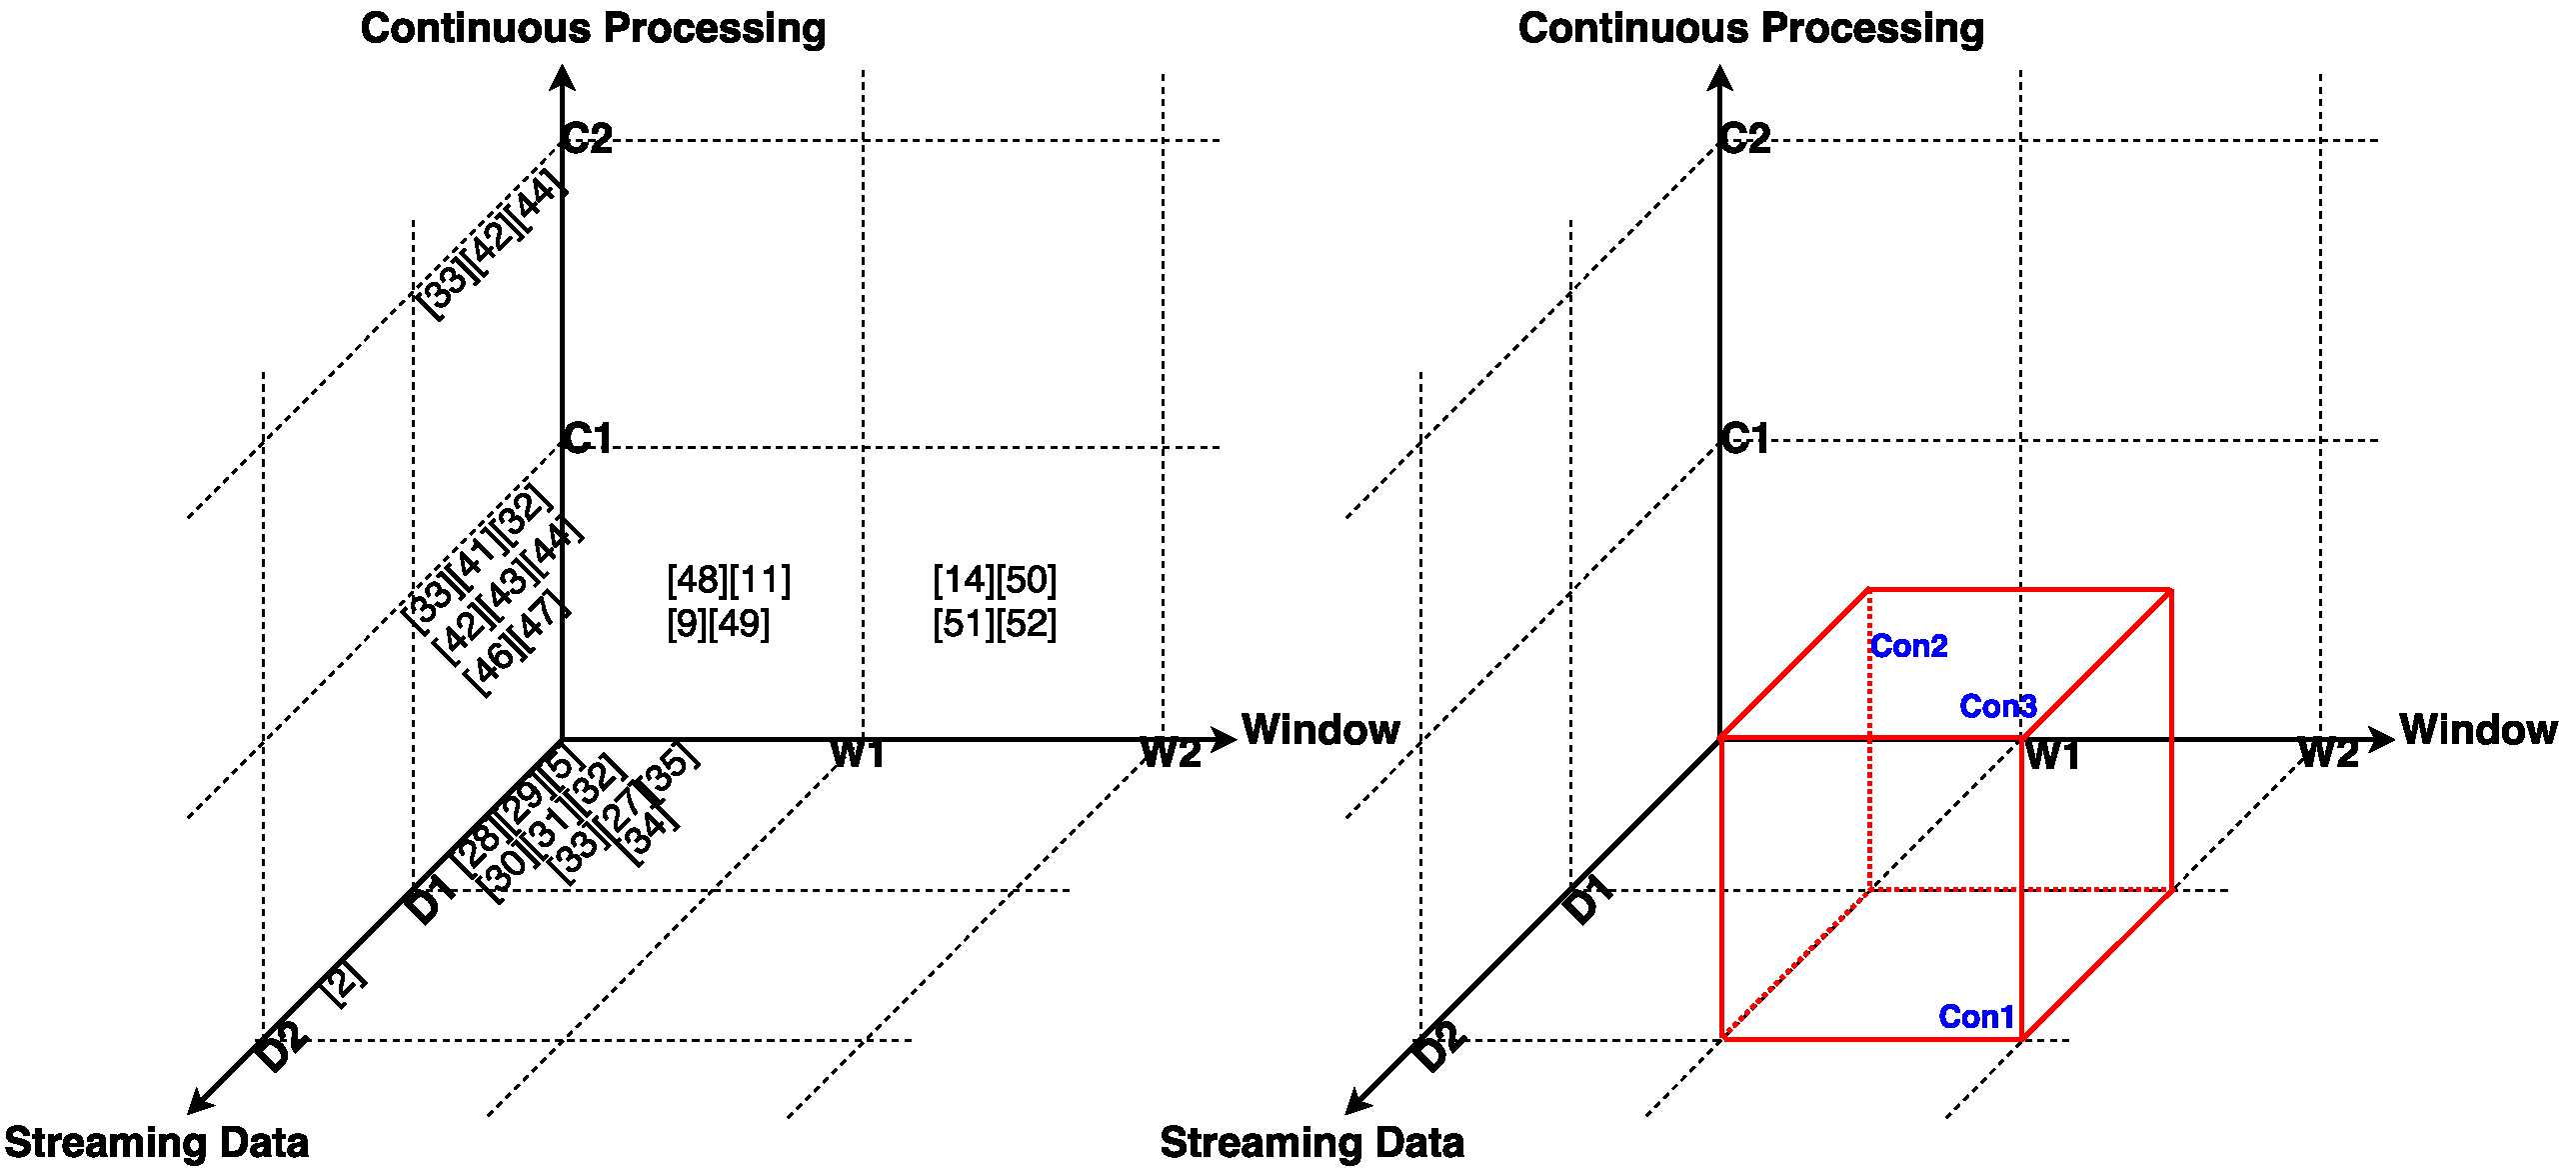
\includegraphics[width=5in]{img/2-rwc.pdf}
    \caption{Contributions in Related Work Space}
    \label{fig:2-rwc}
\end{figure}

I have plotted all the above-mentioned related work in this chapter in Figure \ref{fig:2-rwc} with three dimensions of  ``continuous processing'', ``window'' and ``streaming data''.
On the \textit{continuous processing} axis: 
Point C1 denotes ``continuous processing engine'';
Point C2 denotes ``continuous query language''.
On the \textit{window} axis:
Point W1 denotes ``window semantics and window operational semantics'';
Point W2 denotes ``window management strategies''.
On the \textit{streaming data} axis:
Point D1 denotes ``streaming data semantic modeling (RDF stream)'';
Point D2 denotes ``streaming data orderings''.

It turns out that this figure is very helpful to illustrate and understand where the related work is. 
For example, work located in the plane of C1-D1 is about continuous processing engines that process RDF streams. 
There are some empty areas, which doesn't necessarily mean there is no work. 
The related work is definitely not an exhaust list, but are more related to this dissertation. 

Figure \ref{fig:2-rwc} also shows where my contributions can fit into this 3D space, which is the red cube. 
Contribution 1 models the data importance with the data ordering.
Contribution 2 focuses on continuous processing architecture for RDF streams, and leverages some amount of data orderings and window management strategies. 
Contribution 3 focuses on not only continuous processing for RDF streams, generalizing the semantic importance, but also enabling to take a wide range of streaming data, ontologies, queries, and window management strategies.
%%%%%%%%%%%%%%%%%%%%%%%%%%%%%%%%%%%%%%%%%%%%%%%%%%%%%%%%%%%%%%%%%%%% 
%                                                                 %
%                            CHAPTER Three                        %
%                                                                 %
%%%%%%%%%%%%%%%%%%%%%%%%%%%%%%%%%%%%%%%%%%%%%%%%%%%%%%%%%%%%%%%%%%% 
 
\chapter{SEMANTIC IMPORTANCE} 
\blfootnote{Portions of this chapter previously appeared as: Rui Yan, Mark T Greaves, William P. Smith, Deborah L. McGuinness 2016. ``Remembering the Important Things: Semantic Importance in Stream Reasoning." Stream Reasoning 2016 Workshop, International Semantic Web Conference 2016} 
Timely producing query results from processing infinite streams requires efficient methods.
Usually, the answers to a query are hidden in the heterogeneous streams where not all of the data items are used \cite{mileo2013streamrule}. 
An ideal scenario is where all the data items contain the necessary information for answering the query.
For example, registering the query ``select ?s ?p ?o where \{?s ?p ?o\}'' in the stream yields all the streaming data.
Speaking from a practical perspective, this ideal scenario is not common, thus it becomes very critical to employ some efficient algorithms to produce timely and correct outputs from stream reasoning applications.

Streaming data is processed with a window, whose view of the entire data stream is limited by the window size. 
Even though some systems maintain a synopses of the overall stream, the synopses will grow in size as time goes by, which can increasingly consume the storage and computing resources. 
Thus, there is a need for smart and flexible window management strategies that allow identifying, preserving the necessary data items as well as evicting unnecessary data items in the window. 
The strategies also need to be computationally cheap and easy to implement. 

This chapter introduces the notion of semantic importance, which models the importance of the streaming data from its various orderings.
It also covers how window management strategies can be created with semantic importance, as well as how system performance is positively affected by semantic importance. 
%
\section{Semantic Importance}

\begin{figure}[!htbp]
	\centering
	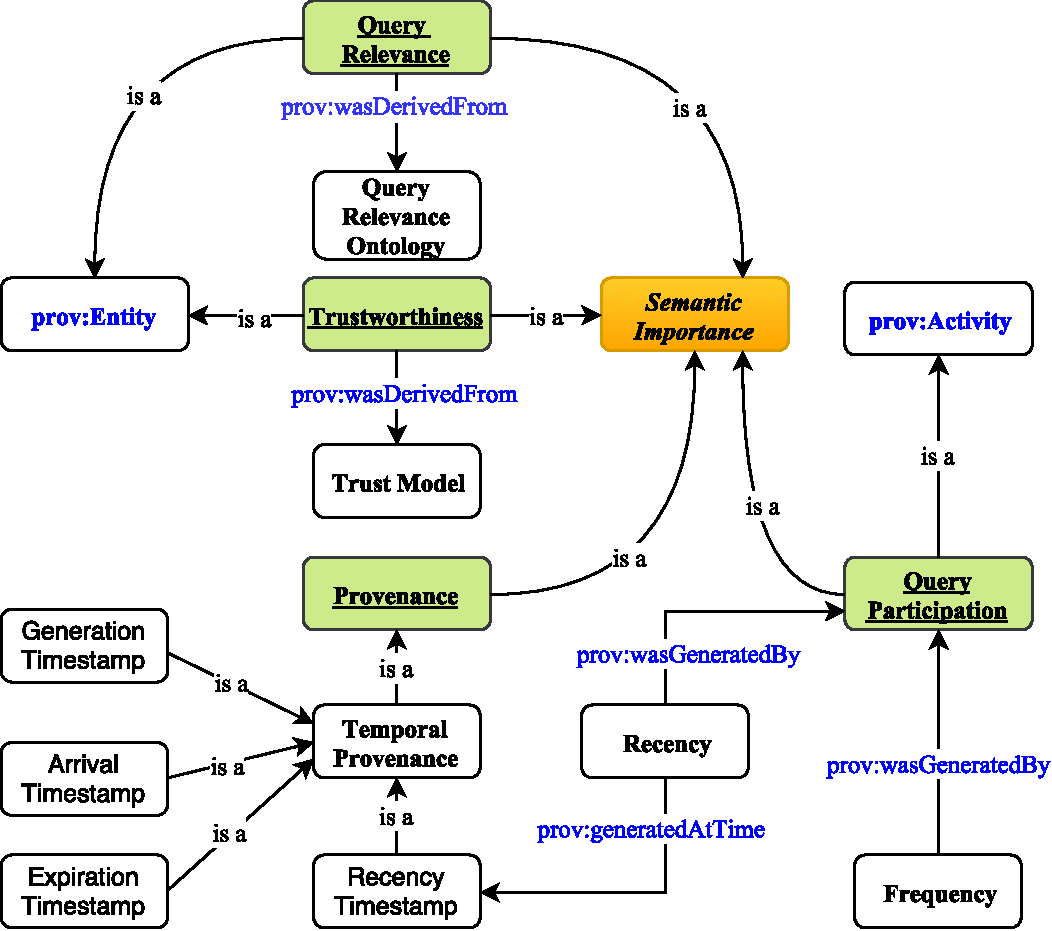
\includegraphics[width=5in]{img/3-si.pdf}
	\caption{Semantic Importance Conceptual Model}
	\label{fig:3-si} 
\end{figure}

For the concept of semantic importance to be relevant, it needs to be the case that not all of the data in the window will contribute equally to the query result \cite{mileo2013streamrule}. 
Given this, the ability to specifically identify the most important data and utilize it effectively is critical for improving stream reasoning system performance. 
So, the question is, can we differentiate and identify effective metrics for use in enabling this task? 
Specifically, in Figure \ref{fig:1-seew}, in order to get the correct answer at $t_{2}$, we need to find a principled and general way to keep $\largetriangleup_{A}$, $\times^{\circ}_{A}$ and wait for $\largecircle_{A}$ to arrive. 
Determining that $\largetriangleup_{A}$, $\times^{\circ}_{A}$ and $\largecircle_{A}$ are more important than other data items is an intuitive observation for a human to make. 
Our goal is to formalize certain parts of this task of judging the relative importance of different streaming data items and use those as the foundation of an ordering relation that can be used for window management.
To do this, I present semantic importance.

\textbf{Semantic importance is defined as an extensible conceptual model that describes the importance of the streaming data by leveraging various streaming data orderings.}
re
Such data orderings are not limited to logical orderings, but also query participation, provenance, and trustworthiness, etc. 
Semantic importance is represented in a priority vector \cite{saaty2003decision}, with elements ordered according to a preference function.
For example, priority vector $V_{p} = [x, y, z]$ has three elements $x, y,$ and $z$.
$x$ is preferred to $y$, and $x, y$ is each preferred to $z$.
The lefter the element is placed, the more preferential the element is.  
There is no restriction on the number of vector elements. 
The traits of the priority vector allow us to consider multiple semantic importance metrics simultaneously while preserving the ability to prioritize some selecting metrics. 

Figure \ref{fig:3-si} shows the conceptual model of semantic importance. 
This conceptual model leverages some concepts from Prov-O \cite{lebo2013prov} to describe the inter-class relationships. 
It is modeled by data orderings, which currently include four aspects: provenance, query participation, trustworthiness, and query relevance.
Each aspect will be introduced in details below.
%
\subsection{Provenance}

\begin{figure}[!htbp]
	\centering
    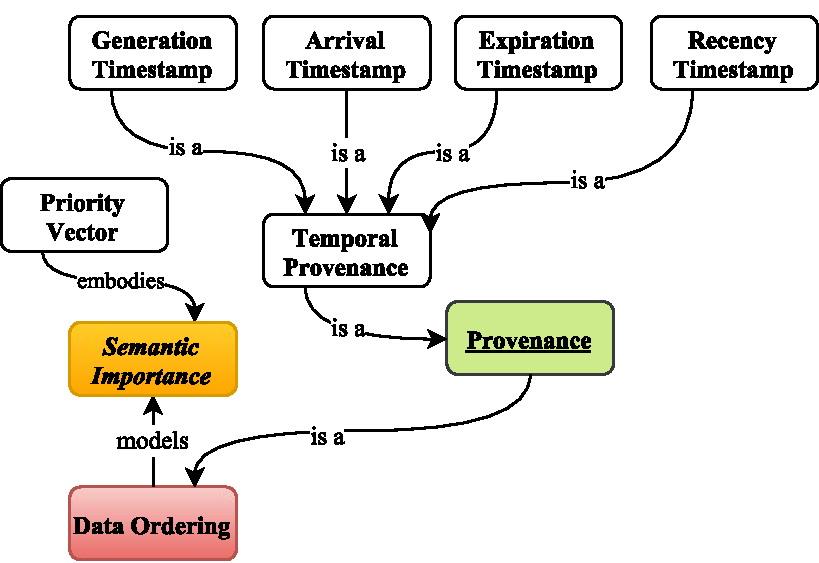
\includegraphics[width=5in]{img/3-sip.pdf}
    \caption{Semantic Importance - Provenance}
    \label{fig:3-sip}
\end{figure}

Provenance is a factor in judging the importance of a streaming data item \cite{gao2010survey}.
This dissertation takes its definition from a foundation paper \cite{ram2009new} in data provenance, 
where \textbf{``provenance is defined as a set of n-tuples: what, when, where, how, who, which, and why.''}
There are several alternate definitions, but this one will suit the dissertation goal since it is a representative definition that includes the extensibility with other definitions. 
It provides the directions to extend provenance aspect with other perspectives such as ``what'', ``where'' or ``how''. 
In the current model, logical provenance\footnote{It is also referred as temporal provenance.} is included and is corresponding to ``when'' aspect in the definition.
This model can certainly go beyond that in the dissertation future work but ``when'' is really what should be started from, because I want to show it for the silent logical assumption.

Even though this dissertation focuses on ``when'' aspect, other types of provenance can also be expanded. 
For example, ``where'' can possibly include the geographical information of the data, whereas ``who'' can possibly refer to the agent that performs some actions. 
In Chapter 5, the soccer offside offense use case leverages positional data as the where-provenance, as well as the players' sensor id as who-provenance. 
The expansion of the provenance aspect will be as one of the future of this dissertation.

There are four branches following the logical provenance.
Generation timestamp ($\tau_{g}$) is assigned by the streaming source, and describes when the data is generated.
Arrival timestamp ($\tau_{a}$) is assigned by the processing system, and describes when the data arrives at the system.
Expiration timestamp ($\tau_{e}$) is assigned by either the processing system or the streaming source, and describes when the data expires.
Recency timestamp ($\tau_{qp}$) is assigned by the system, and is associated with the query participation recency.
For example, priority vector $[\tau_{a}]$ contains $\tau_{a}$ as the only aspect to describe the data importance, and this is the silent logical assumption.
$[\tau_{e}, \tau_{qp}, \tau_{a}]$ uses three aspects to describe the data importance. 
%
\subsection{Query Participation}

\begin{figure}[!htbp]
	\centering
    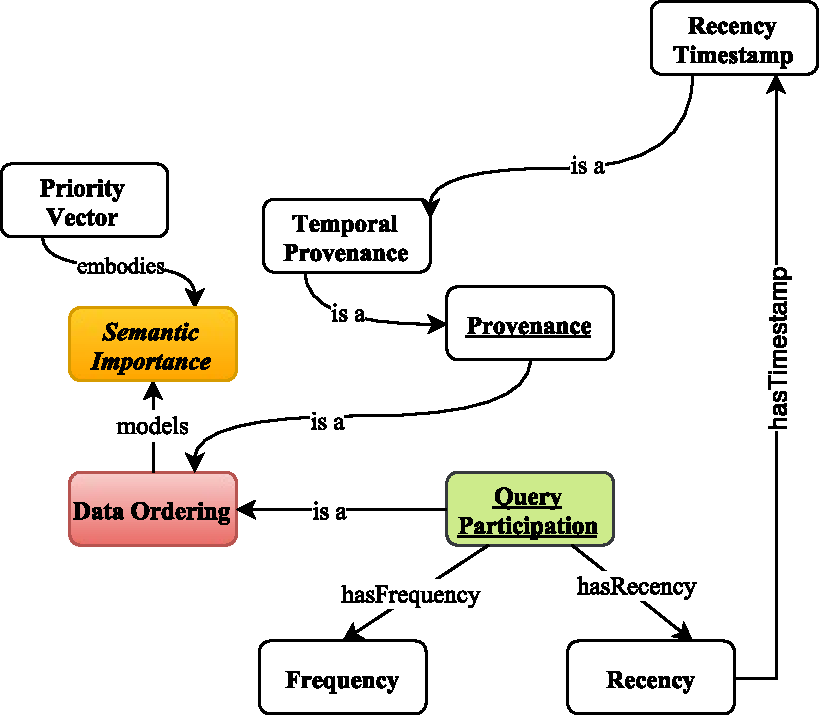
\includegraphics[width=5in]{img/3-siqp.pdf}
    \caption{Semantic Importance - Query Participation}
    \label{fig:3-siqp}
\end{figure}

\textbf{Query participation is defined as: data items participate in a query if they contain necessary information used by the query engine to return non-empty answers.}
Two query participation aspects are frequency and recency.
Frequency ($f_{qp}$) is an integer value that describes how many times a data item participates in the query, 
and recency ($\tau_{qp}$) is a timestamp that describes the most recent time-point for a data item participating in the query.

\begin{figure}[!htbp]
	\centering
    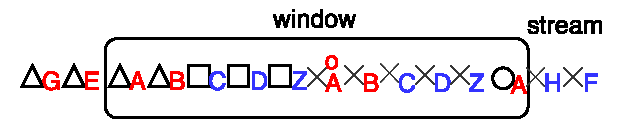
\includegraphics[width=5in]{img/3-siqpe.pdf}
    \caption{Query Participation Example}
    \label{fig:3-siqpe}
\end{figure}

To further explain the definition of query participation, let us consider the example in Figure \ref{fig:3-siqpe}.
We will continue to use the data stream of the soccer offside running example and Table \ref{tab:icons}. 
As mentioned in the previous section, Player A commits an offside offence if he/she is an attacker ($\largetriangleup_{A}$), is at offside position ($\times^{\circ}_{A}$) and involves in an active play ($\largecircle_{A}$) at some time point t.
At this point, since all of the necessary data items are present in the window, the query ``who commits an offside offence'' will be answered. 
This example illustrates that not all of the data items in the window will convey the necessary information that can be used to answer the query. 
The reason why the answer for the query is non-empty is because of the complete presence of $\largetriangleup_{A}$, $\times^{\circ}_{A}$ and $\largecircle_{A}$ at the current active window.
Thus, we say that $\largetriangleup_{A}$, $\times^{\circ}_{A}$ and $\largecircle_{A}$ participate in the query, while others (such as $\largetriangleup_{B}$, $\largesquare_{D}$ or $\times_{B}$) do not. 

\begin{table}[!htbp]
	\centering
    \caption{Updated Query Participation Frequency and Recency}
    \label{tab:uqpfr}
    \begin{tabular}{|c||c|c|c|c|c|c|c|c|c|c|c|} \hline
    	data item & $\largetriangleup_{A}$ & $\largetriangleup_{B}$ & $\largesquare_{C}$ & $\largesquare_{D}$ & $\largesquare_{Z}$ & $\times^{\circ}_{A}$ & $\times_{B}$ & $\times_{C}$ & $\times_{D}$ & $\times_{Z}$ & $\largecircle_{A}$ \\ \hhline{|=#=|=|=|=|=|=|=|=|=|=|=|}
		$f_{qp}$ & 1 & 0 & 0 & 0 & 0 & 1 & 0 & 0 & 0 & 0 & 1 \\ \hline
        $\tau_{qp}$ & $\tau_{qp1}$ & - & - & - & - & $\tau_{qp1}$ & - & - & - & - & $\tau_{qp1}$ \\ \hline 
    \end{tabular}
\end{table}

Assume that it is the first time to execute the query, thus all data items should have $f_{qp} = 0$, and no $\tau_{qp}$. 
When the query result is returned, data items' statistics will be updated. 
Table \ref{tab:uqpfr} shows that $\largetriangleup_{A}$, $\times^{\circ}_{A}$ and $\largecircle_{A}$'s $f_{qp}$ increases by 1, and $\tau_{qp}$ becomes $\tau_{qp1}$.
They have the same $\tau_{qp}$ because they participate in the query at the time $t = \tau_{qp1}$. 
Other data items' $f_{qp}$ and $\tau_{qp}$ remain unchanged. 
%
\subsection{Trustworthiness}

\begin{figure}[!htbp]
	\centering
    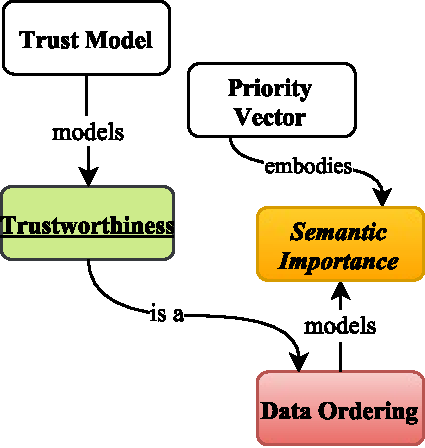
\includegraphics[width=5in]{img/3-sit.pdf}
    \caption{Semantic Importance - Trustworthiness}
    \label{fig:3-sit}
\end{figure}

Different work models trustworthiness in different ways.
For example, in \cite{bertino2009challenge}, trustworthiness is modeled as ``the probability of one data item to be correct''. 
Other work models data trustworthiness from perspectives of data quality \cite{juran1999quality}, \cite{kahn2002information}, \cite{prince2004semiotic}, \cite{wand1996anchoring}, semantic integrity \cite{date2004database} and reputation techniques \cite{kamvar2003eigentrust}, \cite{levien2009attack}. 
The concept of trustworthiness can be very broad, which makes it very suitable to be included in the semantic importance conceptual model. 
In this dissertation, \textbf{trustworthiness is defined as ``worthy of confidence''} \cite{trustdef2018}.
However, in order to let the concept of trustworthiness to be useful and comparable, this work relies on the related literatures on trustworthiness modeling. 

Semantic importance doesn't emphasize on any specific trust models.
But for the sake of convenient processing, data items should be stamped with a numerical value as a trust score ($t^{tm}_{s}$) by a selected trust model ($tm$). 
%
\subsection{Query Relevance}

\begin{figure}[!htbp]
	\centering
    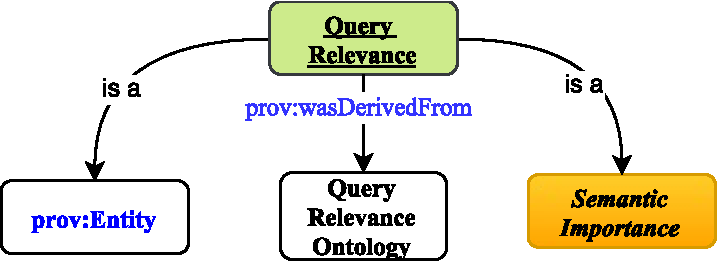
\includegraphics[width=5in]{img/3-siqr.pdf}
    \caption{Semantic Importance - Query Relevance}
    \label{fig:3-siqr}
\end{figure}
Query relevance ties specific knowledge about queries and data into window management using formal semantics. 
It is \textbf{defined as the description of data items' potential to answer the query}.
Query relevance shares the similar assumption from \cite{mileo2013streamrule}: 
``not all raw data from the input stream might be relevant for complex reasoning''.
This description is query-informed, and encoded in an ontology called ``query relevance ontology''.
The query relevance ontology is provided by the users, and enables query relevance as shown in Figure \ref{fig:3-siqr}.
For the concepts in the query relevance ontology to be useful, it is usually constructed with existing concepts in the background domain ontology, which is shown in Figure \ref{fig:3-siqreo}.

\begin{figure}[!htbp]
	\centering
    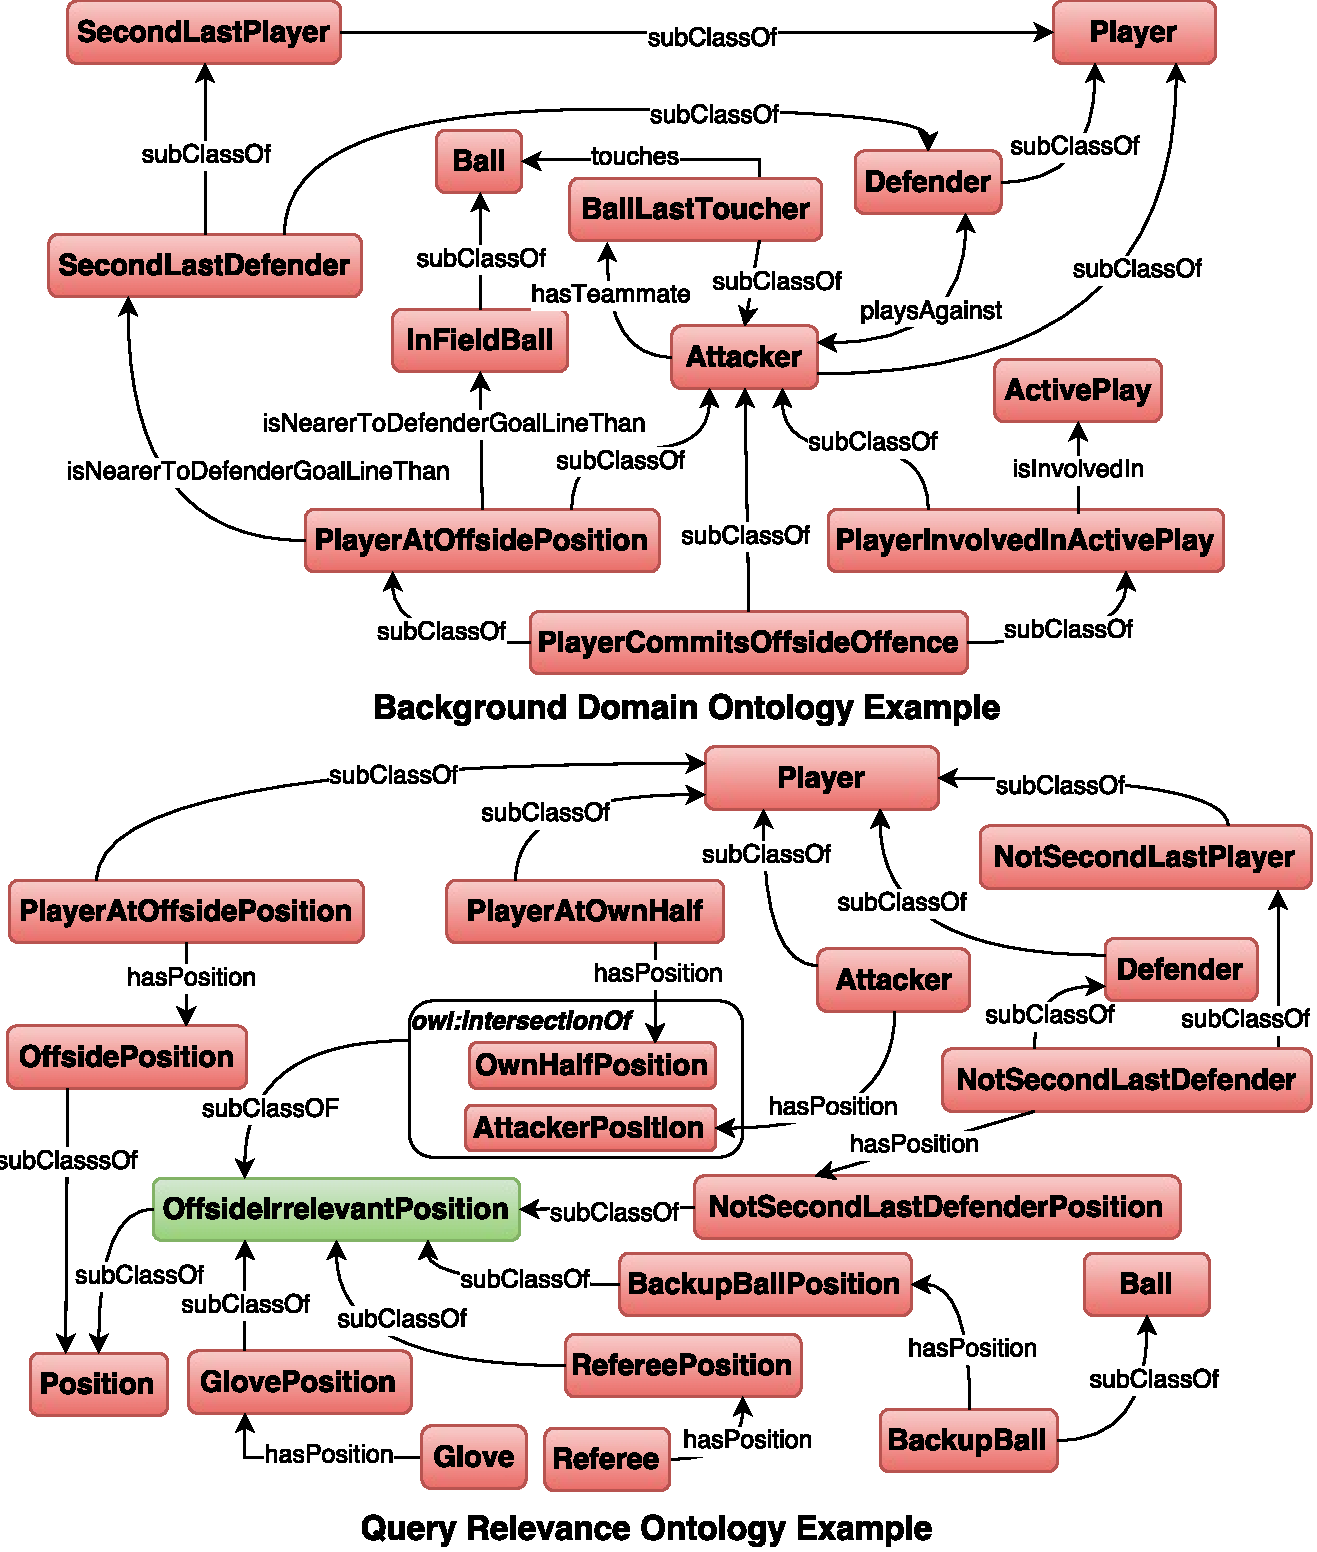
\includegraphics[width=5in]{img/3-siqreo.pdf}
    \caption{Query Relevance Ontology}
    \label{fig:3-siqreo}
\end{figure}

In Figure \ref{fig:3-siqreo}, all the red boxes are concepts encoded in the background domain ontology of soccer, which contains the general knowledge about the overall soccer domain. 
The background ontology can not only answer the query of ``who commits an offside offence'', but also ``who are attackers'', ``which team is controlling the ball'' and ``who is challenged by whom'', etc. 
the only concept in the query relevance ontology is marked in green, which is \textbf{OffsideIrrelevantPosition}. 
But the query relevance ontology only provides details of query relevance for one specific query, which in this case is ``who commits an offside offence''. 

In the Query Participation Section, we have already mentioned that not all of the data will be participating in the query.
The idea of query relevance is to encode the knowledge of human literacy about the query. 
In soccer offside detection, humans know that the positions of the offensive players at their own half will not participate in the query according to the soccer offside definition. 
It is easy to ignore such irrelevant data for linesmen during officiating the game since they are aware of this knowledge. 
However, in order to let the machines acquire this knowledge, users should provide a formalized representation and load it into the system. 
As what will be shown in Chapter 6, the benefits to deploy query relevance include reducing memory consumption and response time, as well as improving precision and throughput. 
The reason is because it allows the system to concentrate on a smaller portion of the original data, which still contains enough necessary information for query answering. 
Thus, for query relevance ontology of ``who commits an offside offence'', the concept of \textbf{OffsideIrrelevantPosition}, which is in green, is constructed in Figure \ref{fig:3-siqreo}. 
This \textbf{OffsideIrrelevantPosition} contains the positions of gloves, referees, defenders other than the second last defender, offensive players at their own half, etc. 
With this query relevance ontology, instances of \textbf{OffsideIrrelevantPosition} (such as  $\times_{B}$, $\times_{C}$ and $\times_{D}$ in Figure \ref{fig:3-siqre}) can be captured and filtered by the system via executing a filtering SPARQL query. 

\begin{figure}[!htbp]
	\centering
    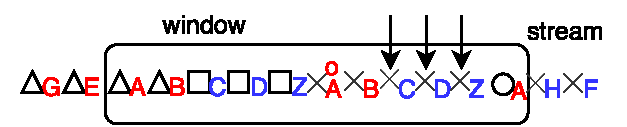
\includegraphics[width=5in]{img/3-siqre.pdf}
    \caption{Query Relevance Example}
    \label{fig:3-siqre}
\end{figure}

The system can be totally blind or literate about streaming data query relevance, depending on whether or not a query relevance query/ontology is deployed, as well as how comprehensive the knowledge of the streaming data is encoded. 
For example, in Figure \ref{fig:3-siqre}, $\largesquare_{D}$ is irrelevant as a defender can never commit an offside offence. 
If such knowledge is also included in the query relevance ontology, the query relevance ontology becomes more comprehensive, and more irrelevant data can be filtered out. 
As the consequences of the query relevance ontology, data items pointed by arrows are not relevant to the current query and thus can be filtered out of the window.


There are several general principles in order to prepare query relevance ontologies.
First, to understand the target and requirements of the use case. 
Since query relevance ontology is domain-specific, and is possibly dependent on the background ontology, understanding what is expected out of the use case can provide a clear ontology construction goal. 
Second, to understand the data, meaning to know what data is useful or useless to the use case.
The patterns of relevant data will then be composed and encoded in the ontology.
Third, keep in mind that query relevance ontology will not work for different queries, since it is so customized to one query in one use case.
%
\section{Comparison Rule}
The semantic importance model encodes the aspects to provide a multi dimensional view on importance.
For example, $[\tau_{e}, \tau_{a}]$ uses expiration timestamp ($\tau_{e}$) and arrival timestamp ($\tau_{a}$) to describe data importance; while $[t^{tm}_{s}, f_{qp}]$ uses trustworthiness and query participation frequency to describe data importance. 
However, in order to enable order-awareness, there should be a comparable rule to be used to rank the data according to its importance. 
This rule, named semantic importance comparison rule, evaluates the data importance by comparing all dimensions of a priority vector for each data item. 
The comparison rule uses comparable operator ``$<$'', ``$>$'' and ``$==$'' to compare priority vector elements. 
The semantics of these comparable operators are defined in Table \ref{tab:cos}.

\begin{table*}[!htbp]
	\centering
	\caption{Comparable Operator Semantics}
	\label{tab:cos}
	\begin{tabular}{|c|c|c|c|} \hline
		SI & $<$ & $>$ & $==$ \\ \hline
        $\tau_{g}$ & \makecell{if $\tau^{1}_{g}$ is before than $\tau^{2}_{g}$ \\ $\Rightarrow \tau^{1}_{g} < \tau^{2}_{g}$} & \makecell{if $\tau^{1}_{g}$ is after than $\tau^{2}_{g}$ \\ $\Rightarrow \tau^{1}_{g} > \tau^{2}_{g}$} & \makecell{$\tau^{1}_{g}$ is equal to $\tau^{2}_{g}$ \\ $\Rightarrow \tau^{1}_{g} == \tau^{2}_{g}$} \\ \hhline{|=#=|=|=|}
		$\tau_{a}$ & \makecell{if $\tau^{1}_{a}$ is before than $\tau^{2}_{a}$ \\ $\Rightarrow \tau^{1}_{a} < \tau^{2}_{a}$} & \makecell{if $\tau^{1}_{a}$ is after than $\tau^{2}_{a}$ \\$\Rightarrow \tau^{1}_{a} > \tau^{2}_{a}$} & \makecell{if $\tau^{1}_{a}$ is equal to $\tau^{2}_{a}$ \\$\Rightarrow \tau^{1}_{a} == \tau^{2}_{a}$} \\ \hline
		$\tau_{e}$ & \makecell{if $\tau^{1}_{e}$ is before than $\tau^{sys}$ \\ if $\tau^{2}_{e}$ is before than $\tau^{sys}$ \\$\Rightarrow \tau^{1}_{e} < \tau^{2}_{e}$}& \makecell{if $\tau^{1}_{e}$ is after than $\tau^{sys}$ \\ if $\tau^{2}_{e}$ is before than $\tau^{sys}$\\$\Rightarrow \tau^{1}_{e} > \tau^{2}_{e}$} & \makecell{if $\tau^{1}_{e}$ is before than $\tau^{sys}$ \\ if $\tau^{2}_{e}$ is before than $\tau^{sys}$ \\ $\Rightarrow \tau^{1}_{e} == \tau^{2}_{e}$ \\if $\tau^{1}_{e}$ is after than $\tau^{sys}$\\if $\tau^{2}_{e}$ is after than $\tau^{sys}$\\$\Rightarrow \tau^{1}_{e} == \tau^{2}_{e}$} \\ \hline
        $\tau_{qp}$ & \makecell{if $\tau^{1}_{qp}$ is before than $\tau^{2}_{qp}$\\ $\Rightarrow \tau^{1}_{qp} < \tau^{2}_{qp}$} & \makecell{if $\tau^{1}_{qp}$ is after than $\tau^{2}_{qp}$ \\ $\Rightarrow \tau^{1}_{qp} > \tau^{2}_{qp}$} & \makecell{if $\tau^{1}_{qp}$ is equal to $\tau^{2}_{qp}$ \\ $\Rightarrow \tau^{1}_{qp} == \tau^{2}_{qp}$} \\ \hline
        $f_{qp}$ & $f^{1}_{qp} < f^{2}_{qp}$ & $f^{1}_{qp} > f^{2}_{qp}$ & $f^{1}_{qp} == f^{2}_{qp}$ \\ \hline
        $qrf$ & false $<$ true & true $>$ false & \makecell{true == true \\false == false} \\ \hline
        $t^{tm}_{s}$ & $t^{tm}_{s1} < t^{tm}_{s2}$ & $t^{tm}_{s1} > t^{tm}_{s2}$ & $t^{tm}_{s1} == t^{tm}_{s2}$ \\ \hline        
	\end{tabular}
\end{table*}

In Table \ref{tab:cos}, $\tau$ represents timestamps, $\tau^{sys}$ denotes current system time, $t^{tm}_{s}$ refers to trust score by a trust model $tm$, $qrf$ represents query relevance filter. 
When query relevance is included in the importance description, a data filtering SPARQL query will be executed. 

When comparing priority vectors\footnote{Only priority vectors with same amount of elements can be compared.}, the leftmost element will be compared first. 
If there is a tie for this element, the second element then will be compared, and so on. 
This is because the priority vector requires its elements to be ordered according to a preference function, as a consequence, the more preferred elements are placed on more lefter side. 
For example, if a data item is associated with an explicit expiration timestamp ($\tau_{e}$), the priority vector $[\tau_{e}]$ will consider unexpired data to be important.
If the data frequency of the query participation ($f_{qp}$) is included, the priority vector $[\tau_{e}, f_{qp}]$ emphasizes $\tau_{e}$ over $f_{qp}$ to guarantee that one unexpired data item is more important than another.
For all unexpired data, what is more important is which participates more frequently in the query.
Expired data becomes less important no matter how frequent its query participation is.
By explicitly characterizing the importance for each data item in the stream, order-awareness can be realized by ranking the semantic importance priority vectors via the following algorithm:

\begin{algorithm}[!htbp]
  priority vectors $v_{1} = [x_{1}, ... , x_{n}]$, $v_{2} = [y_{1}, ... , y_{n}]$ \;
  int i = 0 \;
  \While{$i < n$} {
	  \uIf{$x_{i} > y_{i}$}{
    	return $v_{1} > v_{2}$ \;
  	  }
	  \uElseIf{$x_{i} < y_{i}$}{
    	return $v_{1} < v_{2}$ \;
 	  }
  	  \uElse{
    	i++ \;
  	  } 	
  }
  \uIf{i == n} { 
  	return $v_{1} == v_{2}$ \;  
  }
\caption{Semantic Importance Comparison Algorithm}
\end{algorithm}
%
\section{Window Management Strategies}
A sliding window is defined as a finite subset of the stream \cite{botan2010secret}. 
It has two parameters, a window size (width) that determines how much data a window can contain; 
a window step (slide) that is the distance between two consecutive windows. 
A window has different types \cite{barbieri2010querying}, \cite{patroumpas2006window}.
For all details about windows and operational semantics, please refer to Chapter 2. 

As mentioned in the Introduction Section, the silent logical assumption that older information becomes irrelevant at some point \cite{barbieri2010stream}, \cite{stuckenschmidt2010towards} is very popular in stream reasoning \cite{golab2003processing}, \cite{barbieri2010deductive}.
Based on this silent logical assumption, the dominant window management strategy is first in first out (FIFO). 
This strategy consumes the most recent data based on the window step. 
In order to guarantee identical window size during processing, the amount of data to be evicted should be strictly identical with that of data to be consumed.
The data to be evicted is usually the oldest.

In order to illustrate how semantic importance enabled window management strategies can manage the data items in the window, we will use a running example with a physical sliding window of a size of four tuples, and a step of one tuple. 
Six strategies, including FIFO, will be shown in detail about the way and differences they manage streaming data in the window.

\textbf{FIFO}:
First In First Out (FIFO) describes data importance with a single arrival timestamp ($\tau_{a}$) from the logical provenance aspect. 
Its priority vector is $[\tau_{a}]$.

\begin{figure}[!htbp]
	\centering
    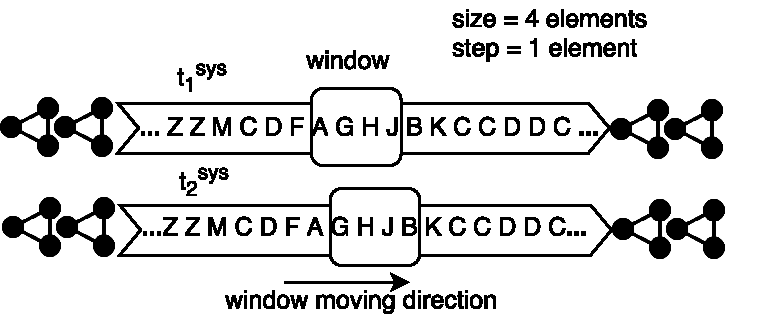
\includegraphics[width=5in]{img/3-sififo.pdf}
    \caption{FIFO Management Strategy}
    \label{fig:3-sififo}
\end{figure}

In Figure \ref{fig:3-sififo}, data \textbf{arrives} in a logical order such that $\tau^{A}_{a} < \tau^{G}_{a} < \tau^{H}_{a} < \tau^{J}_{a} < \tau^{B}_{a}$.
At $t^{sys}_{1}$, items A, G, H, and J are in the window. 
At $t^{sys}_{2}$, as window proceeds, A is evicted so as to consume B. 
Given the arrival order, the data rankings at $t^{sys}_{1}$ and $t^{sys}_{2}$ are shown in Table \ref{tab:fifo}.
Data gets re-ranked as window moves, and data ranked at the bottom will be evicted.

\begin{table}[!htbp]
\centering
\caption{Data Ranking Under FIFO}
\label{tab:fifo}
\begin{tabular}{|c|c|c||c|c|c|}
\hline
\multicolumn{3}{|c||}{$t^{sys}_{1}$} & \multicolumn{3}{c|}{$t^{sys}_{2}$} \\ \hhline{|===#===|}
rank & data & $\tau_{a}$ & rank & data & $\tau_{a}$ \\ \hhline{|=|=|=#=|=|=|}
1 & J & $\tau^{J}_{a}$ & 1 & B & $\tau^{B}_{a}$ \\ \hline
2 & H & $\tau^{H}_{a}$ & 2 & J & $\tau^{J}_{a}$ \\ \hline
3 & G & $\tau^{G}_{a}$ & 3 & H & $\tau^{H}_{a}$ \\ \hline
4 & A & $\tau^{A}_{a}$ & 4 & G & $\tau^{G}_{a}$ \\ \hline
\end{tabular}
\end{table}

\textbf{FEFO}:
First Expired First Out (FEFO) describes data importance with a single expiration timestamp ($\tau_{e}$) from the logical provenance aspect. 
Its priority vector is $[\tau_{e}]$.

\begin{figure}[!htbp]
	\centering
    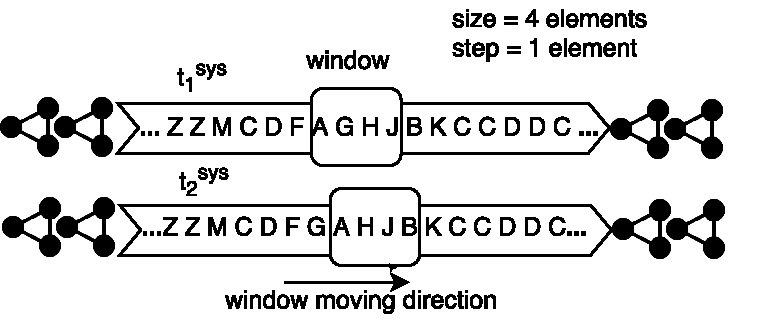
\includegraphics[width=5in]{img/3-sifefo.pdf}
    \caption{FEFO Management Strategy}
    \label{fig:3-sifefo}
\end{figure}

In Figure \ref{fig:3-sifefo}, at $t^{sys}_{1}$, data \textbf{arrives} in a logical order such that $\tau^{A}_{a} < \tau^{G}_{a} < \tau^{H}_{a} < \tau^{J}_{a} < \tau^{B}_{a}$, \textbf{expires}\footnote{We use the ``$==$'' semantics from Table \ref{tab:cos}. Note that the value of $\tau^{A}_{e}$, $\tau^{J}_{e}$ and $\tau^{H}_{e}$ are not necessarily numerically equal.} in a logical order such that $\tau^{G}_{e} < t^{sys}_{1} < \tau^{B}_{e} < t^{sys}_{2} < \tau^{A}_{e} == \tau^{J}_{e} == \tau^{H}_{e}$.
At $t^{sys}_{1}$, items A, G, H, and J are in the window, G is expired.
At $t^{sys}_{2}$, G is evicted to consume B, which will be evicted next. 
Note that even though G arrives later than A, G is evicted because of FEFO management strategy,
and even though B is the latest data item, it is also an expired data item, thus needs to be evicted. 
Data rankings at $t^{sys}_{1}$ and $t^{sys}_{2}$ are listed in Table \ref{tab:fefo}. 
The data item ranks at the bottom will be evicted. 

\begin{table}[!htbp]
\centering
\caption{Data Ranking Under FEFO}
\label{tab:fefo}
\begin{tabular}{|c|c|c||c|c|c|}
\hline
\multicolumn{3}{|c||}{$t^{sys}_{1}$} & \multicolumn{3}{c|}{$t^{sys}_{2}$} \\ \hhline{|===#===|}
rank & data & $\tau_{e}$ & rank & data & $\tau_{e}$ \\ \hhline{|=|=|=#=|=|=|}
1 & H, J, A & $\tau^{H}_{e}$, $\tau^{J}_{e}$, $\tau^{A}_{e}$ & 1 & H, J, A & $\tau^{H}_{e}$, $\tau^{J}_{e}$, $\tau^{A}_{e}$ \\ \hline
2 & G & $\tau^{G}_{e}$ & 2 & B & $\tau^{B}_{e}$ \\ \hline
\end{tabular}
\end{table}

\textbf{LFU}:
Least Frequently Used (LFU) is a classic caching algorithm \cite{crp2018}, but not commonly used in the window management.
LFU describes the data importance with a single query participation frequency ($f_{qp}$) from the query participation aspect. 
Its priority vector is $[f_{qp}]$.

\begin{figure}[!htbp]
	\centering
    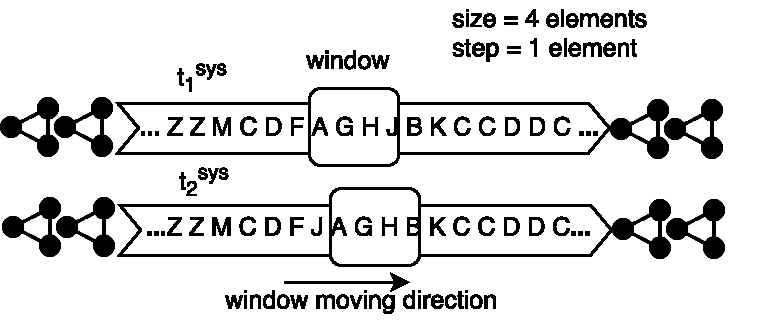
\includegraphics[width=5in]{img/3-silfu.pdf}
    \caption{LFU Management Strategy}
    \label{fig:3-silfu}
\end{figure}

In Figure \ref{fig:3-silfu}, data \textbf{arrives} in a logical order such that $\tau^{A}_{a} < \tau^{G}_{a} < \tau^{H}_{a} < \tau^{J}_{a} < \tau^{B}_{a}$. 
As soon as the data arrives in the window, its $f_{qp}$ is initialized to be 0.
$f^{X}_{qp}$ will increase by 1 if the data item X participates in the query once.
At $t^{sys}_{1}$, assuming that $f^{A}_{qp} = 3$, $f^{G}_{qp} = 2$, $f^{H}_{qp} = 0$, $f^{J}_{qp} = 0$. 
Since $t^{H}_{qp} = t^{J}_{qp} = 0$, both H and J rank at the bottom in Table \ref{tab:lfu}. 
Either H or J will be evicted in an undecided way because of the window step is 1 tuple. 
In Figure \ref{fig:3-silfu}, let's tentatively evict J to consume B. 
After query is executed, assuming that B participates in the query thus $f^{B}_{qp}$ becomes 1.
Then, data items in the window get re-ranked at $t^{sys}_{2}$.
Since $f^{H}_{qp}$ is 0 and the smallest, data item H will be ranked at the bottom and evicted next. 

\begin{table}[!htbp]
\centering
\caption{Data Ranking Under LFU}
\label{tab:lfu}
\begin{tabular}{|c|c|c||c|c|c|}
\hline
\multicolumn{3}{|c||}{$t^{sys}_{1}$} & \multicolumn{3}{c|}{$t^{sys}_{2}$} \\ \hhline{|===#===|}
rank & data & $f_{qp}$ & rank & data & $f_{qp}$ \\ \hhline{|=|=|=#=|=|=|}
1 & A & 3 & 1 & A & 4 \\ \hline
2 & G & 2 & 2 & G & 3 \\ \hline
3 & H, J & 0 & 3 & B & 1 \\ \hline
4 & - & - & 4 & H & 0 \\ \hline
\end{tabular}
\end{table}

\textbf{FE-LFU-FO}:
First Expired Least Frequently Used First Out (FE-LFU-FO) is a more complex window management strategy. 
It describes the data importance with the expiration timestamp ($\tau_{e}$) and the query participation frequency ($f_{qp}$).
Its priority vector is $[\tau_{e}, f_{qp}]$, which emphasizes $\tau_{e}$ over $f_{qp}$. 

\begin{figure}[!htbp]
	\centering
    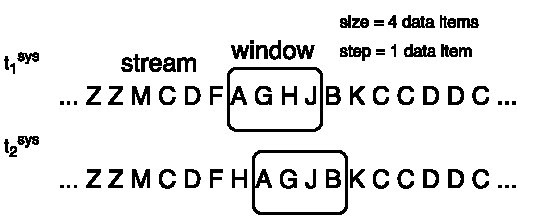
\includegraphics[width=5in]{img/3-sifelfufo.pdf}
    \caption{FE-LFU-FO Management Strategy}
    \label{fig:3-sifelfufo}
\end{figure}

In Figure \ref{fig:3-sifelfufo}, assuming that data arrives in a logical order such that $\tau^{A}_{a} < \tau^{G}_{a} < \tau^{H}_{a} < \tau^{J}_{a} < \tau^{B}_{a}$, and expires in an order such that $\tau^{H}_{e} < t^{sys}_{1} < t^{sys}_{2} < \tau^{G}_{e} == \tau^{J}_{e} == \tau^{A}_{e} == \tau^{B}_{e}$.
At $t^{sys}_{1}$, we can compare data items priority vector according to the comparison rule. 
Since $[\tau^{H}_{e}, 4] < [t^{sys}_{1}, -] < [\tau^{G}_{e}, 0] < [\tau^{J}_{e}, 2] < [\tau^{A}_{e}, 3]$, H ranks at the bottom thus evicted even though it participated most in the query. 
At $t^{sys}_{2}$, $[t^{sys}_{2}, -] < [\tau^{G}_{e}, 0] == [\tau^{B}_{e}, 0] < [\tau^{J}_{e}, 3] < [\tau^{A}_{e}, 4]$.
Table \ref{tab:felfufo} shows the data rankings. 
At $t^{sys}_{2}$, both B and G are ranked at the bottom, thus either will be evicted due to the window step. 

\begin{table}[!htbp]
\centering
\caption{Data Ranking Under FE-LFU-FO}
\label{tab:felfufo}
\begin{tabular}{|c|c|c|c||c|c|c|c|}
\hline
\multicolumn{4}{|c||}{$t^{sys}_{1}$} & \multicolumn{4}{c|}{$t^{sys}_{2}$} \\ \hhline{|====#====|}
rank & data & $\tau_{e}$ & $f_{qp}$ & rank & data & $\tau_{e}$ & $f_{qp}$ \\ \hhline{|=|=|=|=#=|=|=|=|}
1 & A & $\tau^{A}_{e}$ & 3 & 1 & A & $\tau^{A}_{e}$ & 4 \\ \hline
2 & J & $\tau^{J}_{e}$ & 2 & 2 & J & $\tau^{J}_{e}$ & 3 \\ \hline
3 & G & $\tau^{G}_{e}$ & 0 & 3 & B,G & $\tau^{B}_{e}$, $\tau^{G}_{e}$ & 0 \\ \hline
4 & H & $\tau^{H}_{e}$ & 4 & 4 & - & - & - \\ \hline
\end{tabular}
\end{table}

\textbf{LFU-FE-FO}:
Least Frequently Used First Expired First Out (LFU-FE-FO), just like FE-LFU-FO, describes the data importance with $\tau_{e}$ and $f_{qp}$. 
Its priority vector $[f_{qp}, \tau_{e}]$, albeit has the same elements as FE-LFU-FO's $[\tau_{e}, f_{qp}]$, it ranks data items in a totally different way. 

\begin{figure}[!htbp]
	\centering
    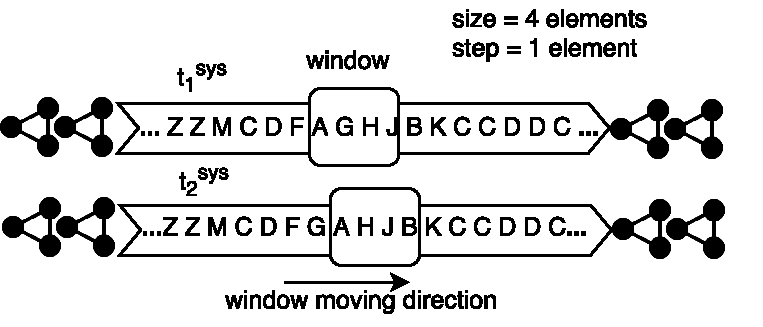
\includegraphics[width=5in]{img/3-silfufefo.pdf}
    \caption{LFU-FE-FO Management Strategy}
    \label{fig:3-silfufefo}
\end{figure}

In Figure \ref{fig:3-silfufefo}, assuming that data arrives in a logical order such that $\tau^{A}_{a} < \tau^{G}_{a} < \tau^{H}_{a} < \tau^{J}_{a} < \tau^{B}_{a}$, and expires in a logical order such that $\tau^{H}_{e} < t^{sys}_{1} < t^{sys}_{2} < \tau^{G}_{e} == \tau^{J}_{e} == \tau^{A}_{e} == \tau^{B}_{e}$. 
Together with Table \ref{tab:lfufefo}, at $t^{sys}_{1}$, $[-, t^{sys}_{1}] < [0, \tau^{G}_{e}] < [2, \tau^{J}_{e}] < [3, \tau^{A}_{e}] < [4, \tau^{H}_{e}]$. 
G is ranked at the bottom thus will be evicted.
However, H is ranked at the top even though H is expired. 
What is even worse is that H has the most query participation frequency, that almost guarantees that H will be at the top forever, resulting in invalid answers.
At $t^{sys}_{2}$, $[-, t^{sys}_{2}] < [0, \tau^{B}_{e}] < [3, \tau^{J}_{e}] < [4, \tau^{A}_{e}] < [5, \tau^{H}_{e}]$.
H, A and J's query participation frequencies increase by 1, while B doesn't participate in the query.
Thus B is ranked at the bottom and will be evicted. 

From this example, we can see that even though the window management strategies formed by combining different semantic importance aspects can be various, what's crucial behind it is to careful design the combination so that the strategy can manage data in a legit way. 

\begin{table}[!htbp]
\centering
\caption{Data Ranking Under LFU-FE-FO}
\label{tab:lfufefo}
\begin{tabular}{|c|c|c|c||c|c|c|c|}
\hline
\multicolumn{4}{|c||}{$t^{sys}_{1}$} & \multicolumn{4}{c|}{$t^{sys}_{2}$} \\ \hhline{|====#====|}
rank & data & $f_{qp}$ & $\tau_{e}$ & rank & data & $f_{qp}$ & $\tau_{e}$ \\ \hhline{|=|=|=|=#=|=|=|=|}
1 & H & 4 & $\tau^{H}_{e}$ & 1 & H & 5 & $\tau^{H}_{e}$ \\ \hline
2 & A & 3 & $\tau^{A}_{e}$ & 2 & A & 4 & $\tau^{A}_{e}$ \\ \hline
3 & J & 2 & $\tau^{J}_{e}$ & 3 & J & 3 & $\tau^{J}_{e}$ \\ \hline
4 & G & 0 & $\tau^{G}_{e}$ & 4 & B & 0 & $\tau^{B}_{e}$ \\ \hline
\end{tabular}
\end{table}

\textbf{FE-LFU-FI-FO}:
First Expired Least Frequently Used First In First Out (FE-LFU-FI-FO) uses the expiration timestamp ($\tau_{e}$), query participation frequency ($f_{qp}$) and arrival timestamp ($\tau_{a}$) to describe the data importance.
Its priority vector is $[\tau_{e}, f_{qp}, \tau_{a}]$, which contains three elements.

\begin{figure}[!htbp]
	\centering
    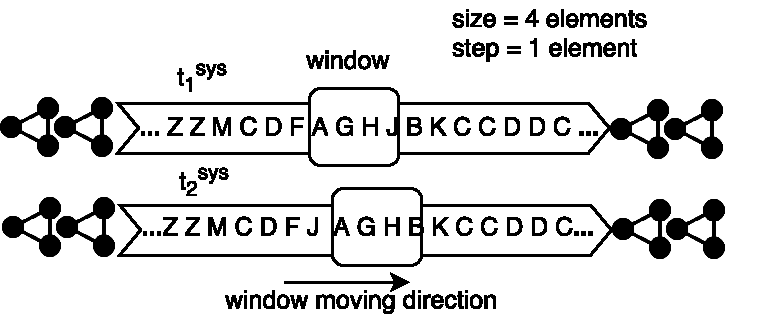
\includegraphics[width=5in]{img/3-sifelfufifo.pdf}
    \caption{FE-LFU-FI-FO Management Strategy}
    \label{fig:3-sifelfufifo}
\end{figure}

In Figure \ref{fig:3-sifelfufifo}, assuming that data arrives in a logical order such that $\tau^{A}_{a} < \tau^{G}_{a} < \tau^{H}_{a} < \tau^{J}_{a} < \tau^{B}_{a}$, and expires in a logical order such that  $\tau^{J}_{e} < t^{sys}_{1} < \tau^{G}_{e} < t^{sys}_{2} < \tau^{H}_{e} == \tau^{A}_{e} == \tau^{B}_{e}$.
At $t^{sys}_{1}$, $[\tau^{J}_{e}, 6, \tau^{J}_{a}] < [t^{sys}_{1}, -, -] < [\tau^{G}_{e}, 0, \tau^{G}_{a}] < [\tau^{H}_{e}, 1, \tau^{H}_{a}] < [\tau^{A}_{e}, 4, \tau^{A}_{a}]$. 
At $t^{sys}_{2}$, $[\tau^{G}_{e}, 0, \tau^{J}_{a}] < [t^{sys}_{2}, -, -] < [\tau^{B}_{e}, 0, \tau^{B}_{a}] < [\tau^{H}_{e}, 2, \tau^{H}_{a}] < [\tau^{A}_{e}, 5, \tau^{A}_{a}]$. 
With these orderings, data is ranked as in Table \ref{tab:felfufifo}. 
Data ranked at the bottom will be evicted. 

\begin{table}[!htbp]
\centering
\caption{Data Ranking Under FE-LFU-FI-FO}
\label{tab:felfufifo}
\begin{tabular}{|c|c|c|c|c||c|c|c|c|c|}
\hline
\multicolumn{5}{|c||}{$t^{sys}_{1}$} & \multicolumn{5}{c|}{$t^{sys}_{2}$} \\ \hhline{|=====#=====|}
rank & data & $\tau_{e}$ & $f_{qp}$ & $\tau_{a}$ & rank & data & $\tau_{e}$ & $f_{qp}$ & $\tau_{a}$ \\ \hhline{|=|=|=|=|=#=|=|=|=|=|}
1 & A & $\tau^{A}_{e}$ & 4 & $\tau^{A}_{a}$ & 1 & A & $\tau^{A}_{e}$ & 5 & $\tau^{A}_{a}$ \\ \hline
2 & H & $\tau^{H}_{e}$ & 1 & $\tau^{H}_{a}$ & 2 & H & $\tau^{H}_{e}$ & 2 & $\tau^{H}_{a}$ \\ \hline
3 & G & $\tau^{G}_{e}$ & 0 & $\tau^{G}_{a}$ & 3 & B & $\tau^{B}_{e}$ & 0 & $\tau^{A}_{a}$ \\ \hline
4 & J & $\tau^{J}_{e}$ & 6 & $\tau^{J}_{a}$ & 4 & G & $\tau^{G}_{e}$ & 0 & $\tau^{G}_{a}$ \\ \hline
\end{tabular}
\end{table}

The above six strategies are certainly not an exhaustive list of all the window management strategies that semantic importance can enable. 
The point is provide both examples and evidence that semantic importance can not only enable classic FIFO strategy, but also smarter and more flexible strategies. 
FE-LFU-FO and LFU-FE-FO strategies manage data differently even though their priority vectors have same elements. 
Other possible strategies with priority vectors such as $[t^{tm1}_{s}, \tau_{e}, \tau_{a}]$, $[qrf, t^{tm1}_{s}, t^{tm2}_{s}, \tau_{e}, \tau_{a}]$ are also very similar to implement.
%
\section{Window Semantics}
Semantic importance is an interesting idea to pursuit because it brings a better concept of what to forget, so as to shrink the window size during processing the gigantic data streams.
However, forgetting based on FIFO is only logical.
The silent logical assumption is probably a good reflection of logically-oriented-only importance.
The soccer example shows that the ``importance'' is a deeper notion, a more domain specific notion, which cannot be adequately modeled merely by time alone. 
One motivation of this dissertation is to take the notion of importance into semantics by bringing the domain into the computation with an efficient way. 
This requires not only to model the importance of the data, but also to extend the current sliding window semantics that is related to the silent logical assumption. 

What will be shown later illustrates why it is important to extend the window semantics in order to realize the flexible and smart window management strategies.
The method is to re-define the window size and step, as well as to extend the sliding logical window semantics with the lower-bounded landmark window whose lower bound is fixed permanently, and upper bound proceeds. 
This extended window semantics can work well with the semantic importance. 
%
\subsection{Problems in Existing Window Semantics}
``\textbf{A window W over a stream S is a finite subset of S}'' \cite{dindar2013modeling}.
A sliding window has two parameters, size and step, both have been mentioned and defined in related work \cite{beck2015lars}, \cite{dindar2013modeling}, \cite{prud2008sparql}, \cite{botan2010secret}, \cite{arasu2006cql}.
\cite{dindar2013modeling} requires that all windows defined over a stream must have the same size and step, with a restriction that the step could be any value that must be no bigger than the size.
\cite{patroumpas2006window} indicates that physical window step is 1 with the statement that ``... window states are determined only at single-tuple units ...". 
\cite{calbimonte2010enabling} mentions that ``... if the step is larger than the range then the windows sample the stream ...", indicating that the step can be larger than the size. 
As you can see, there are already some differences on how researchers understand and define window semantics. 
Window semantics is important to define a window and managing data.

In this section, I argue that none of the existing window semantics can be adapted when equipping window with management strategies other than FIFO.  
As a result, existing window semantics need to be extended. 

\begin{figure}[!htbp]
	\centering
    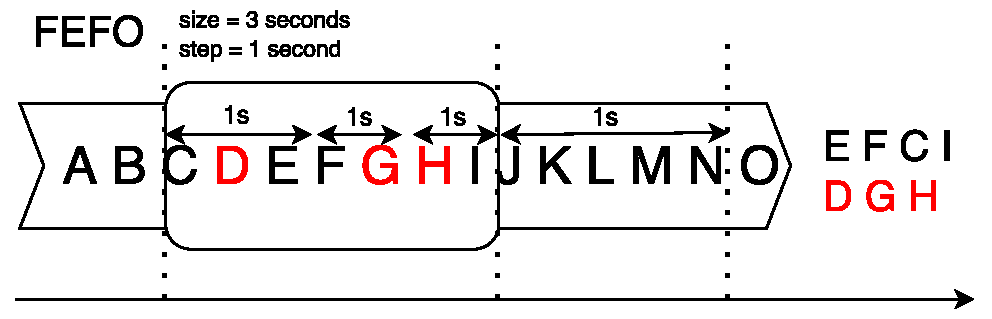
\includegraphics[width=5in]{img/3-wsti.pdf}
    \caption{Logical Sliding Window Under FEFO}
    \label{fig:3-wsti}
\end{figure}

Consider the example in Figure \ref{fig:3-wsti}, which is a logical sliding window under FEFO management strategy, with a size of 3 seconds and a step of 1 second. 
Assume that data items D, G, and H are expired (marked in red), thus ranked at the bottom. 
At this point, window size is still 3 seconds as $t^{I}_{a} - t^{C}_{a} = 3s$, even if D, G, and H are evicted.  
As a consequence, the sliding window will not move as it is still full according to its semantics, so that the continuous processing will be halted. 

\begin{figure}[!htbp]
	\centering
    
\includegraphics[width=5in]{img/3-wstu.pdf}
    \caption{Physical Sliding Window Under FEFO}
    \label{fig:3-wstu}
\end{figure}

In Figure \ref{fig:3-wstu}, a physical (tuple-based) sliding window manages data under FEFO. 
At this moment, data items G and H are expired (marked in red), thus ranked at the bottom. 
However, since the current window semantics defines its step to be 1 and fixed, it can only evict one data item. 
No matter which data item is evicted, a worse case is that the kept expired data item participated in the query, causing the early expiration problem and resulting invalid query answers. 

The two problems above have shown that existing window semantics cannot work well with semantic importance enabled window management strategies. 
The primary reason is that these strategies manage data in a ``data item'' granularity, rather than a simple ``logical'' granularity. 
%
\subsection{Extended Logical Window Semantics}
This dissertation will use the definitions of lower bound ($\tau_{l}$), upper bound ($\tau_{u}$), data stream ($S$), current stream contents ($S(\tau)$), current stream instance ($s_{\tau}$), time domain ($T$) and lower-bounded landmark window ($W^{lbl}$) from \cite{patroumpas2006window}.
A logical lower-bounded landmark window ($W^{lbl}_{\tau}$) is employed as an extended window for a logical sliding window.
For $W^{lbl}_{\tau}$, its $\tau_{l}$ is fixed permanently, while $\tau_{u}$ proceeds as time goes by. 
Figure \ref{fig:3-lw} shows an example of $W^{lbl}_{\tau}$. 

\begin{figure}[!htbp]
	\centering
    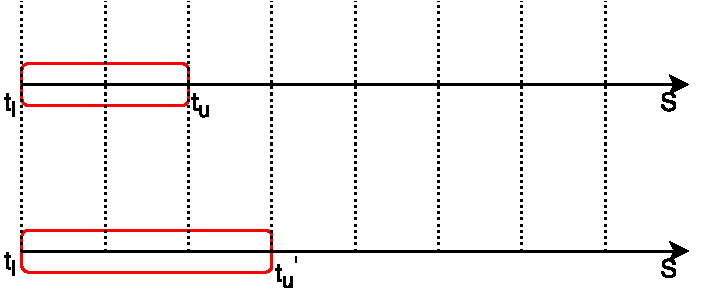
\includegraphics[width=5in]{img/3-lw.pdf}
    \caption{Logical Lower-bounded Landmark Window Example}
    \label{fig:3-lw}
\end{figure}

Rather than defining window size, this dissertation uses the definition from \cite{tangwongsan2015general}:
\textbf{``the instantaneous window size ($n_{\tau}$) at time $\tau$ is defined as the number of tuples in the current active window.''}
With this definition, $W^{lbl}_{\tau}$ window size can vary. 
We define a logical window step for $W^{lbl}_{\tau}$: 
\textbf{window step ($n_{\beta}$) is defined as the number of tuples within next $\beta$ measurement units  \cite{patroumpas2006window} (such as seconds, minutes, etc)}. 

\begin{figure}[!htbp]
	\centering
    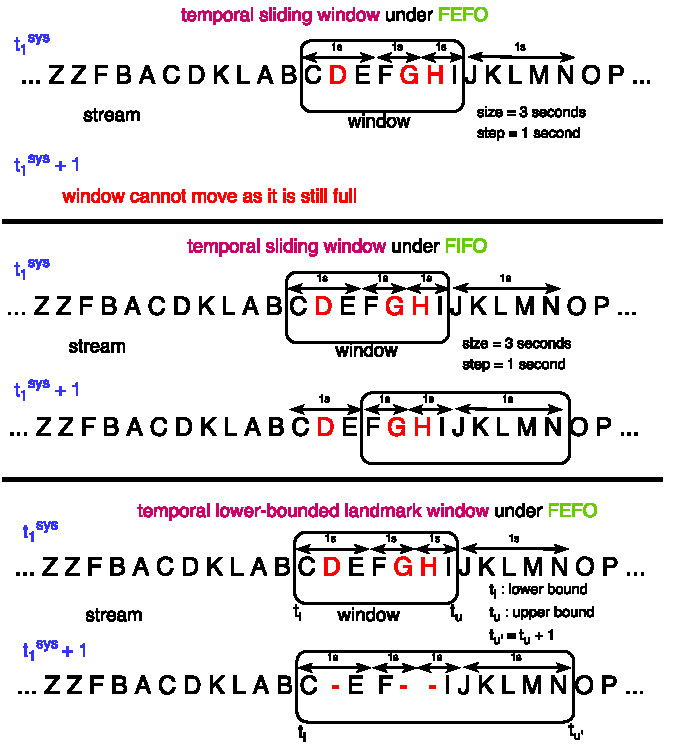
\includegraphics[width=5in]{img/3-psewsti.pdf}
    \caption{Extended Logical Window Semantics Example}
    \label{fig:3-psewsti}
\end{figure}

Figure \ref{fig:3-psewsti} shows how the extended logical window semantics can work with semantic importance enabled window management strategies (such as FEFO) when managing data streams. 
By leveraging the extended logical window semantics from the landmark window, the logical lower-bounded landmark window can continue to proceed after evicting all the expired data.
This is much flexible than a logical sliding window that will have to remove the oldest data under FIFO in order to proceed, which results in removing data items that are still valid (such as C and E in Figure \ref{fig:3-wsti}), and keeping data items that are expired (such as G and H in Figure \ref{fig:3-wsti}). 

\begin{table}[!htbp]
	\centering
	\caption{Window Semantics Example}
	\label{tab:lwsw}
	\begin{tabular}{|c||c|c|}
	\hline
	& \makecell{landmark window \\ under FEFO} & \makecell{sliding window \\ under FIFO} \\ \hhline{|=#=|=|}
	\makecell{window size} & \makecell{$n_{t_{u}} = 7$\\ $n_{t_{u'}} = 9$} & \makecell{2s (7 tuples)\\ 2s (9 tuples)} \\ \hline
	\makecell{query: do both C and N exist \\ in the stream? (early eviction) \\ ground truth: yes } & answer: yes  & answer: no \\ \hline
	\makecell{query: do both G and N exist \\ in the stream? (early expiration) \\ ground truth: no} & answer: no & answer: yes \\ \hline
	\end{tabular}
\end{table}

Table \ref{tab:lwsw} shows the different results of different window semantics. 
We have used the physical window size definition for the landmark window. 
At $t_{u}$ and $t_{u'}$ time in Figure \ref{fig:3-psewsti}, its size is 7 and 9 respectively. 
For the sliding window under FIFO, its size is logical, which is 2 seconds. 
At $t_{1}^{sys}$ and $t_{1}^{sys} + 1$ time in Figure \ref{fig:3-psewsti}, the number of tuples in the sliding window is 7 and 9 respectively.
Thus, even though the landmark window seems to have ``infinite'' growth as its lower bound fixed permanently and its upper bound proceeds, the number of tuples in the window does not necessarily become ``infinite'', thanks to the extended window size definition. 
In this example, the span of the landmark window is 4 seconds, which is larger than the sliding window size of 2 seconds, but the number of tuples in both windows is equal.

The landmark window semantics can also help solve the early eviction and early expiration problem. 
The query ``do both C and N exist in the stream'' will have a false-negative answer from the sliding window under FIFO, as C has to be evicted in order to get N. 
This is an early eviction problem.
In a landmark window with FEFO, C stays as it is not expired, thus can provide the correct answer. 
For the query ``do both G and N exist in the stream'', a false-positive answer will be given by the sliding window under FIFO, as G is expired within the window but cannot be evicted. 
This is an early expiration problem.
The landmark window with FEFO strategy can provide correct result as all the expired data can be evicted without affecting the continuous data consumption and processing.  
%
\subsection{Extended Physical Window Semantics}
Different from the logical window, this dissertation will use a sliding physical (tuple-based) window ($W_{\#}$).
From the window size definition \cite{tangwongsan2015general}, a sliding physical window size $n_{\tau}$ is always a fixed value.
The only part to be extended from the sliding physical window semantics is the step. 
\textbf{The step ($n_{\beta}$) is defined as a variable with its range as ${n_{\beta} = \{\ n_{\beta} \ |\ 0 \leq n_{\beta} \leq n_{\tau}}\}$.}

\begin{figure}[!htbp]
	\centering
    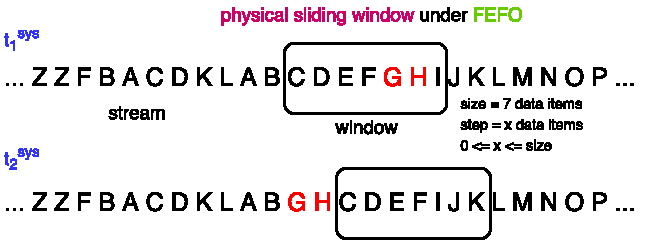
\includegraphics[width=5in]{img/3-psewstu.pdf}
    \caption{Extended Physical Window Semantics Under FEFO}
    \label{fig:3-psewstu}
\end{figure}

Figure \ref{fig:3-psewstu} shows how data can be managed with FEFO, and the extended physical window semantics. 
Since the window step is now a variable no bigger than the window size, evicting data becomes much more flexible: if two data items are expired, both of them will be evicted. 
Thus the window can continue to consume next two new data items. 
If all of the data are expired in the window, then evict all of them to consume next $n_{\tau}$ data items. 
This flexible window step guarantees that all of the unimportant data items are evicted, so as to solve the problems such as the early expiration. 
One thing to note is that, with FEFO, data has to be expired to be evicted.
If all of the data are not expired, the window will not proceed but wait till at least one of them is expired. 
This indicates that the window management strategies manage data differently, and it is crucial to choose a proper strategy to keep the desired data for query.
%
\subsection{Discussion}
\begin{table}[!htbp]
\centering
\caption{Window Semantics Comparison}
\label{tab:wsc}
\begin{tabular}{|c||c|c|}
\hline
 & \begin{tabular}[c]{@{}c@{}}Sliding Window \\ Semantics\end{tabular} & \begin{tabular}[c]{@{}c@{}}Extended Window \\ Semantics\end{tabular} \\ \hhline{|=#=|=|}
\begin{tabular}[c]{@{}c@{}}logical \\ window ($W_{\tau}$)\end{tabular} & sliding window & \begin{tabular}[c]{@{}c@{}}lower-bounded \\ landmark window\end{tabular} \\ \hline
$W_{\tau}$ size & \begin{tabular}[c]{@{}c@{}}fixed.\\ defined with logical \\ measurement units (e.g. 2s)\end{tabular} & \begin{tabular}[c]{@{}c@{}}can vary.\\ defined as $n_{\tau}$, number \\ of tuples at an instantaneous \\ time-point (e.g. 23)\end{tabular} \\ \hline
$W_{\tau}$ step & \begin{tabular}[c]{@{}c@{}}fixed.\\ defined with logical\\  measurement units (e.g. 1s)\end{tabular} & \begin{tabular}[c]{@{}c@{}}fixed.\\ defined as $n_{\beta}$, number \\ of tuples within next $\beta$ \\ measurement units.(e.g. 15)\end{tabular} \\ \hhline{|=#=|=|}
\begin{tabular}[c]{@{}c@{}}physical\\window ($W_{\#}$)\end{tabular} & sliding window & sliding window \\ \hline
$W_{\#}$ size & \begin{tabular}[c]{@{}c@{}}fixed.\\ defined as $n_{\tau}$, number \\ of tuples at an instantaneous \\ time-point (e.g. 23)\end{tabular} & \begin{tabular}[c]{@{}c@{}}fixed.\\ defined as $n_{\tau}$, number \\ of tuples at an instantaneous \\ time-point (e.g. 23)\end{tabular} \\ \hline
$W_{\#}$ step & \begin{tabular}[c]{@{}c@{}}fixed.\\ defined as $n_{\beta}$, number \\ of tuples within next $\beta$ \\ measurement units.(e.g. 15)\end{tabular} & \begin{tabular}[c]{@{}c@{}}variable. \\ $n_{\beta} = \{n_{\beta}\ |\ 0 \leq n_{\beta} \leq n_{\tau}\}$\end{tabular} \\ \hline
\end{tabular}
\end{table}

We discuss why the extended semantics is more general. 
Table \ref{tab:wsc} shows the window semantics comparison between the sliding window and extended window. 
For logical window ($W_{\tau}$), the extended window type becomes the lower-bounded landmark window. 
$W_{\tau}$ size and step are both re-defined with the number of tuples, as opposed to logical measurement units. 
For the physical window, although the same sliding window type is used, its step is extended to be a variable that is no bigger than its window size, as opposed to a previous fixed step. 

The extended window semantics is general, which is reflected by not only the examples shown in Figure \ref{fig:3-psewsti} and Figure \ref{fig:3-psewstu}, but also the fact that sliding logical window can be emulated with the extended window semantics under a proper semantic importance enabled window management strategy. 

\begin{figure}[!htbp]
	\centering
    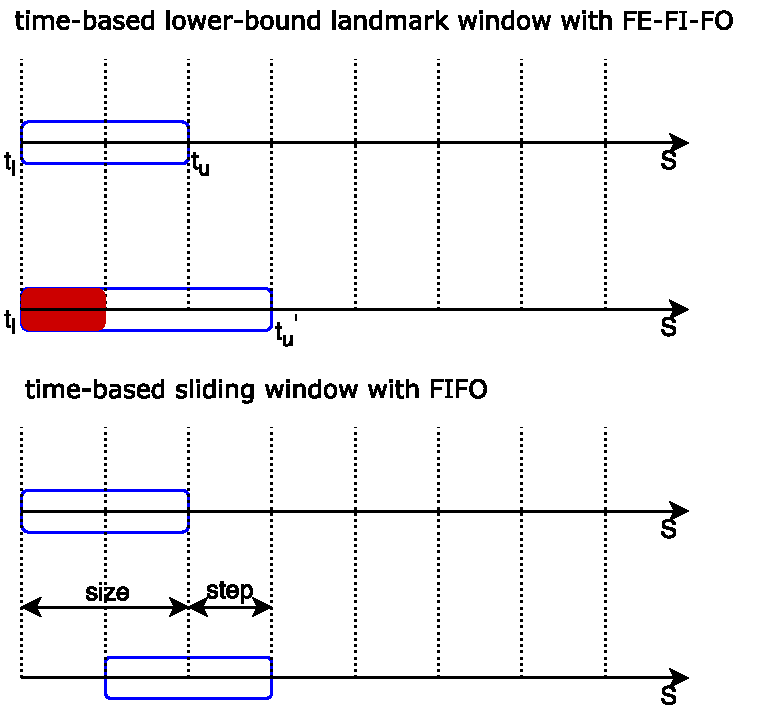
\includegraphics[width=5in]{img/3-lwcsw.pdf}
    \caption{Landmark Window Emulating Sliding Window}
    \label{fig:lwesw}
\end{figure}

Figure \ref{fig:lwesw} illustrates how the extended window semantics can emulate a logical sliding window.
A logical lower-bounded landmark window is managed with FE-FI-FO strategy.
FE-FI-FO is first expired, first in, first out, with a priority vector as $[\tau_{e}, \tau_{a}]$. 
A landmark window simulates a logical sliding window via assigning an expiration timestamp for each data item by adding the arrival timestamp with window initialization length.
This is very similar as how IMaRS \cite{barbieri2010incremental} manages the data. 
When the time reaches $t_{u'}$, the data portion marked in red will be expired in the landmark window, thus evicted. 
The content in the landmark window is the same as the sliding logical window. 

[SIZE 2s STEP 1s] is an example argument to define a logical sliding window in C-SPARQL query language \cite{barbieri2009c}.
Because this definition is only designed for the sliding window, in order to let the extended window semantics to work with the existing continuous query language, there is also a need to align the extended window semantics with the query language window definition.
This portion of work will be covered in Chapter 6. 
%
\section{Summary}
This chapter has introduced the notion of semantic importance, including the definitions, the conceptual model, the comparison rule, window management strategies and window semantics. 
The aspects in the semantic importance conceptual model are not exhaustive, and we encourage people to reuse and extend it. 
In order to make it convenient to reuse semantic importance, I have created an ontology and ground it with real world soccer examples. 
All the details are in Appendix I. 

Currently the model is consisted of two major aspects, the domain agnostic aspects and domain literate aspects. 
Domain agnostic aspects include query participation and provenance.
This is because queries are often executed independently, regardless of data, backgrounds or domains. 
Provenance information is often carried when data is generated. 
Domain literate aspects include trustworthiness and query relevance.
Often the trust models are dependent on the domain. 
For example, you might trust a Japanese friend to be your tour guide in Kobe but probably won't trust this friend to be the guide in New York.
There are lots of trust models that have been proposed and work well in different scenarios. 
Query relevance, in our model, is realized by applying query relevance ontology and query in the system. 
This ontology is different from the background ontology that is usually deployed before the system starts.
The background ontology encodes the essential knowledge of the domain, and is specifically focused on capturing domain knowledge that impacts querying and reasoning to answer questions. 
Query relevance ontology is focused on picking the query informed data for query execution. 
This requires a filtering SPARQL query to be executed before the target query is executed.
This filtering query matches all the irrelevant data that can be classified by some concepts encoded in the query relevance ontology. 
So that the data pool for query execution is smaller to make the target query run faster. 
If data comes with trust scores, it is generally recommended to perform trust filter before the target query runs. 
Again, this is to guarantee that all the data enters into the query phase is trusted.

Using priority vector to encode semantic importance guarantees an efficient and multi-fold ranking.
Together with the comparison rule, semantic importance allows the ranking to consider different aspects comprehensively.
Weighting is a simple and intuitive way to enable ordering. However, the semantic importance is embodied in the priority vector, whose ordering is realized by the position of the item. The leftier a semantic importance item is placed in the priority vector, the more significant it is compared to other items on its right. The comparison rule in Section 3.2 has provided both theory and examples on comparing semantic importance. Weighting is parallel to priority vector. There is also a way to use weighting instead of priority vector to enable ordering, where different weights can be assigned by users who assigns their preferences over semantic importance items, then reduce it into a single value, which can be used to compare and rank data importance. Since the weighting schema is a different way, this dissertation will not focus on it. 

Different window management strategies can be enabled by semantic importance. 
Work such as \cite{dell2013correctness} considers the operation semantics in stream reasoning systems. 
Window operational semantics usually refers to the way how the query is executed in the window, how the data is consumed and evicted. 
For example, C-SPARQL executes the query when the window is full, while CQELS executes when the window receives the new data.

Table \ref{tab:wsc} provides a comparison between the sliding window semantics and extended window semantics.
From what has been shown before, the extended window semantics works seamlessly with the semantic importance enabled window management strategies. 
%
%%%%%%%%%%%%%%%%%%%%%%%%%%%%%%%%%%%%%%%%%%%%%%%%%%%%%%%%%%%%%%%%%%%% 
%                                                                 %
%                            CHAPTER Four                         %
%                                                                 %
%%%%%%%%%%%%%%%%%%%%%%%%%%%%%%%%%%%%%%%%%%%%%%%%%%%%%%%%%%%%%%%%%%% 
 
\chapter{SEQUENTIAL STREAM REASONING ARCHITECTURE}
\blfootnote{*Portions of this chapter previously appeared as: Rui Yan, Brenda Praggastis, William P. Smith, Deborah L. McGuinness. 2016 ``Towards A Cache-Enabled, Order-Aware, Ontology-Based Stream Reasoning Framework." Linked Data on the Web Workshop 2016, 25th World Wide Web Conference 2016}
Most existing stream reasoning systems employ the silent temporal assumption when ``forgetting'' the data, and are not designed to leverage the semantic importance model.
In this chapter, a sequential stream reasoning architecture (SSRA) is proposed to provide an infrastructure to deploy the semantic importance model in stream reasoning systems.

\section{Assumptions}
SSRA shares the common assumptions on ontologies and streaming data, under which existing systems work \cite{barbieri2009c} \cite{barbieri2010c} \cite{barbieri2010execution} \cite{barbieri2010incremental} \cite{anicic2011ep}.
%
\subsection{Ontology}
SSRA follows assumptions for background ontologies:
(1) the stream reasoning system leverages ontologies encoded in OWL \cite{mcguinness2004owl} to support the symbolic reasoning; 
(2) the background ontology is usable, correct, consistent, and provided by the domain experts;
(3) the background ontology is preloaded into the system before the processing starts;
(4) the background ontology doesn't change during the processing. 

A stream reasoning system doesn't necessarily have to employ ontologies to provide reasoning foundations. 
Existing systems \cite{do2011answer} \cite{gebser2012stream} leverage answer set programming (ASP) \cite{gelfond1991classical} to support reasoning.
\cite{mileo2013streamrule} encodes customized rules to enable reasoning.   
However, SSRA chooses to use ontologies for reasoning because they provide a flexible and expressive way to encode knowledge. 
Domain experts are key to composing the ontologies. 
The complexity of the ontology should be determined by the use case requirements. 
The correctness of the ontology is very crucial to determine the query results, as the knowledge for executing the query is solely provided by the background ontology. 
The domain knowledge in the ontologies usually doesn't change (frequently). 
Previous work including \cite{gao2016planning} \cite{ren2010towards} considers the change of the background knowledge.
Their method is to update the background ontology over time.
Between two adjacent updates, the background ontology remains static.
Overall, the assumptions on the background ontologies are reasonable and can be loosened with minimum efforts. 
%
\subsection{Streaming Data}
SSRA follows assumptions for the streaming data: 
(1) the streaming sources encapsulate the streaming data items as RDF stream format, and in unique named graphs;
(2) the streaming sources assign expiration timestamps to streaming data items;
(3) SSRA assigns arrival timestamps for the streaming data.

RDF streams \cite{della2009first} are RDF data annotated with timestamps that are either time-points or time-intervals.
The RDF stream format can be represented as $<\rho, \tau>$, where $\rho$ is an RDF molecule \cite{ding2005tracking}, and $\tau$ is a timestamp denoting the arrival time of $\rho$.
An RDF stream is defined as an ordered sequence of pairs \cite{barbieri2010proposal} \cite{barbieri2009c}, each of which consists of an RDF triple and a monotonically non-decreasing timestamp $\tau$, identified by a unique IRI that is a streaming source locater, and published in a named graph \cite{carroll2005named}.
The above work justifies the assumption of leveraging named graphs in the RDF streams. 

SSRA extends the RDF stream format by adding another timestamp and a unique graph ID.
Thus, an RDF stream is represented by $<\rho,\tau_{a}, \tau_{e}, G>$, where $\rho$ denotes the RDF molecule/statement, $\tau_{a}$ denotes its arrival timestamp, $\tau_{e}$ denotes its expiration timestamp and $G$ denotes its unique graph ID.

Under the silent temporal assumption, the expiration timestamps are assigned by the system via adding arrival timestamps with the logical window size \cite{barbieri2010incremental}. 
Given the information of the window and the system as a priori, the streaming source can assign expiration timestamps as exactly as what the system can do. 
Thus, the assumption on assigning expiration timestamps also cover the situation where the data itself carries the expiration timestamps, or data expires due to the new data arrival at some random time. 
%
\section{Architecture}
SSRA consists of a window and four sequential components: \textit{data consumption}, \textit{query execution}, \textit{result explanation} and \textit{data eviction}.
These four components are executed in a sequential order. 
The execution flow forms a loop to process data streams and to produce query results in a continuous fashion, as it is shown in Figure \ref{fig:4-ssra}. 

\begin{figure}[!htbp]
	\centering
	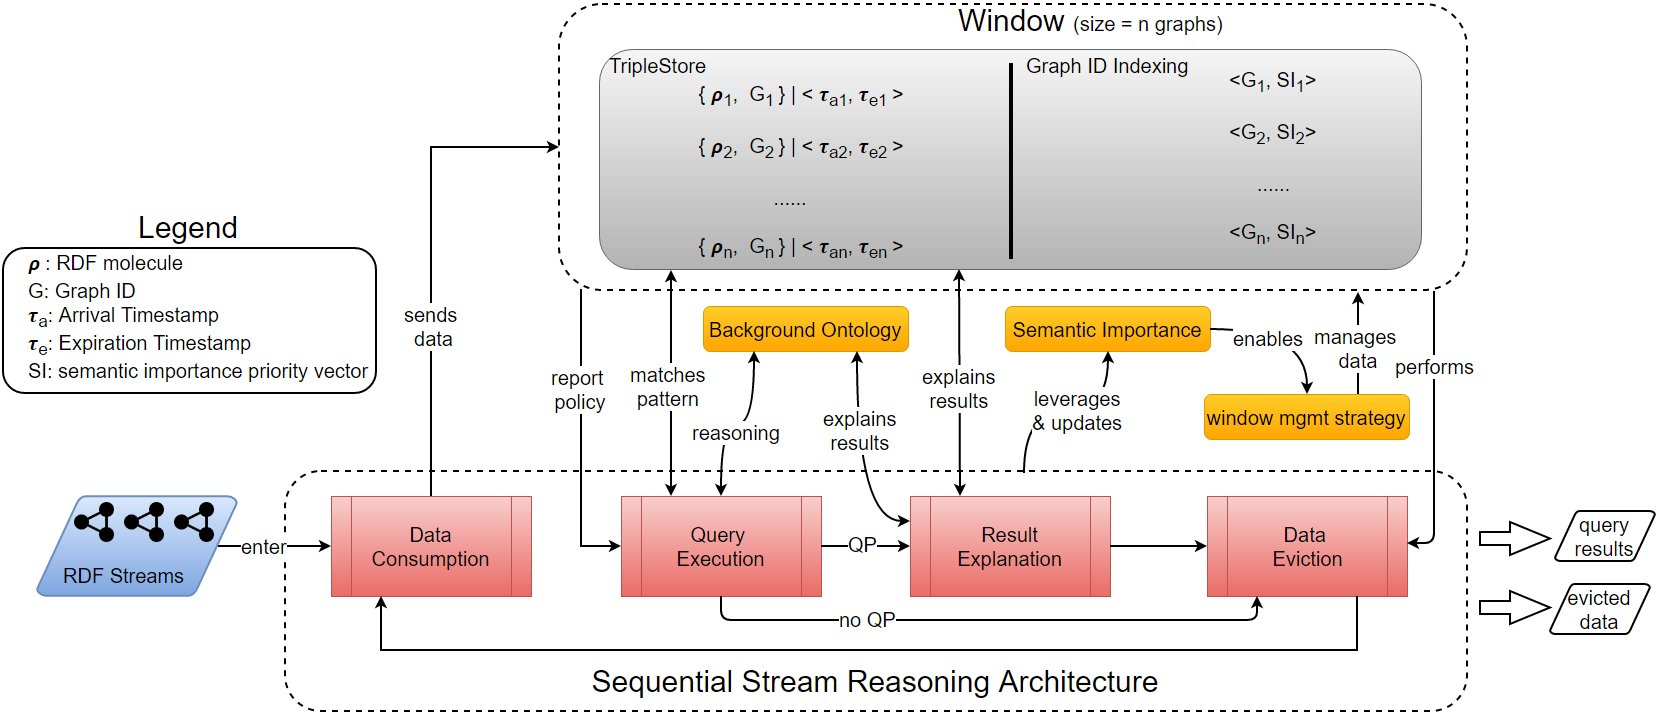
\includegraphics[angle=90,height=7.5in]{img/4-ssra.png}
	\caption{Sequential Stream Reasoning Architecture.}
	\label{fig:4-ssra}
\end{figure}

%
\subsection{Window}
The window is designed with a triple-store that stores the data physically, and a graph ID manager that indexes the data graphs.
The background ontology is preloaded in the window triple-store.
The window receives and keeps the data from the data consumption.
The query is executed in the window with the triple-store query engine, background ontology and the data.
The triple-store also provides the ability to explain the results.
The graph ID manager helps index the data, manage data semantic importance priority vectors and rank the data. 
Coupled with the window management strategies, the graph ID manager can provide the list of data to be evicted from the triple-store.
%
\subsection{Data Consumption}
RDF streams enter SSRA via data consumption component. 
Its behavior is modeled and controlled by both Tick and Report operational semantics from the SECRET model \cite{botan2010secret}.
It consumes data in either a time-driven or tuple-driven way, depending on how the window is defined. 
It can realize different reporting policies as well. 
For example, ``on window close'' policy allows the streaming data enters the window till full before executing the query; 
while ``on content change'' policy allows to execute the query once the content is changed in the window, regardless of window fullness. 
In either policy, it will send the query execution request to the next component.
%
\subsection{Query Execution}
The query in the stream reasoning scenario should be continuous in order to provide proactive answers. 
This requires the query to be preregistered in the system before the data arrival.
SSRA, unlike what existing work does, employs standard SPARQL query.
This is for two reasons:
(1) C-SPARQL \cite{barbieri2009c}, EP-SPARQL \cite{anicic2011ep} and other extended SPARQL require different execution models and syntax that are not compatible.
Even though RSP-QL \cite{dell2014rsp} was proposed later with the goal to unifying the continuous queries, it currently is meant to be a reference model to explain the heterogeneity of stream reasoning engines. 
The execution engine is very challenging to develop as it will have to cover all the C-SPARQL/CQELS/other operational semantics which possibly will lose the responsive performance.
(2) the requirement of ``continuity'' can be easily realized by forming a loop in SSRA, rather than employing some continuous query syntax or execution models. 
In fact, even the continuous SPARQL queries, such as C-SPARQL, need to be translated into the continuous query part (which includes the window and stream information), and the static query part (which is basically the SPARQL query).
Thus, the mechanism of executing a continuous SPARQL query is essentially to execute a translated SPARQL query with associated window and stream definitions.
This is the same as what SSRA does. 

In SSRA, reasoning happens during the query time. 
This provides an advantage that only the necessary entailments for the answer will be computed. 
However, it is worth pointing out that reasoning does not have to happen at the same time as the query does. 
One example is materialization \cite{barbieri2010incremental},  which is performed iteratively: the materialized snapshot of the database is always updated as long as the new data arrives. 
%
\subsection{Result Explanation}
If query participation (QP) is specified, the window needs to know the query participation status of every named graph after the query result is delivered.
Result Explanation Component works in a way to trace back to the provenance of the query result; that is to find which named graphs participated in the query process. 
The result is explained by proof trees\footnote{For an example, please refer to \url{http://docs.stardog.com/\#\_proof\_trees}}.

A(n) (inferred) result can be obtained by both explicit triples and intermediate inferences. 
Only the query participation statistics of those graph IDs belonging to explicit triples will be recorded.

In each run iteration, semantic importance has to be updated so as to re-rank the data. 
Based on different window management strategies, semantic importance is updated differently.
For example, in FEFO strategy, the window is constantly looking for expired data.
The important data is those unexpired. 
If the data expires, it will be moved to the deletion pool for eviction. 
For strategies such as FE-LFU-FO, the window updates semantic importance based on the expiration timestamp and query participation frequency.
If the data is expired, it will be moved to the deletion pool for eviction regardless how frequently it used to participate in the query. 
If the data is not expired, it will be ranked based on frequency.
Other window management strategies will follow the same pattern to update the semantic importance.
One thing to notice is that, rules to update semantic importance is only determined by window management strategies, without human-in-the-loop required.
%
\subsection{Data Eviction}
This component evicts the named graphs ranked at the bottom in the window. 
Depending on different window management strategies, data is evicted differently.
For example, FEFO collects one statistic -- the expired data count, $E_{d}$. 
$E_{d}$ increments by one if a named graph is expired.
FE-LRU-FO collects two statistics -- $E_{d}$ and the most recent query participation timestamps, $\tau_{qp}$, for every named graph. 
$E_{d}$ increases by one if a named graph is expired.
Every valid named graph's old $\tau_{qp}$ is replaced with the corresponding new $\tau_{qp}$.
FE-LFU-FO collects two statistics -- $E_{d}$ and every named graph's query participation frequency counts, $\delta_{qp}$, in the latest cycle.
$E_{d}$ increments by one if a named graph is expired, and every valid named graph's total query participation frequency counter, $f_{qp}$, adds the corresponding $\delta_{qp}$. 
The window re-ranks the data immediately after semantic importance is updated. 
%
\section{Implementation}
In SSRA, the most important part is the window. 
All of the components are constantly interacting with the window.
SSRA implements and configures the window as follows.

\textbf{Triple-store}:
SSAR has been implemented using two off-the-shelf triple-stores: AllegroGraph v5.0.2\footnote{http://franz.com/agraph/allegrograph/} and Stardog v4.0 RC3\footnote{http://stardog.com/}. 
Both provide Java APIs and step-by-step tutorials. 
AllegroGraph is an efficient modern graph database by Franz Inc\footnote{http://franz.com/}. 
It supports up to OWL2 RL reasoning and full SPARQL 1.1. 
Stardog is a graph database by Complexible Inc\footnote{http://complexible.com/}. 
It supports up to OWL2 DL \& rule-based reasoning and SPARQL 1.1.
Stardog supports reasoning explanation via proof trees, but AllegroGraph does not. 
Free versions of both products are used.

The SPARQL drop argument is leveraged to fully remove named graphs from the window. 
We avoid using the SPARQL delete argument because it only removes the statements in the graphs, not the graph ids.
This will pollute the window's graph ID manager in Figure \ref{fig:4-ssra}.
Stardog supports both memory \& disk-based databases, while AllegroGraph only supports disk-based databases. 
We have implemented three prototypes, focusing on Stardog memory \& disk-based and AllegroGraph disk-based window stream reasoning system. 
As mentioned above, the reasoning abilities of these two triple-stores are different.
In order to perform a fair comparison, we use a query that only requires RDFS reasoning.
%

\textbf{Window Type:}
In this implementation, we employ the sliding physical window with a fixed size $l$.
This is because, according to our extended window semantics, a physical window's size is a fixed value and thus controllable. 
In our extended semantics, a physical window step is a variable that is less than the window size. 
Thus, in order to control the window step ($d$), it is set to be 25\%, 50\%, 75\% and 100\% of $l$ to see if the amount of data to be evicted has any influence on the query results.
%
\section{Evaluation}
The stream reasoning community has not yet come to consensus on the best method to evaluate stream reasoning applications. 
SRbench\cite{zhang2012srbench} was proposed as a general benchmark system designed to test streaming RDF engines. 
LSBench\cite{le2012linked} was proposed to focus on assessing different Linked Stream Data (LSD) applications' capabilities. 
CSRBench\cite{dell2013correctness} was proposed with a special emphasis on the effects of operation semantics for stream reasoning applications. 
More recently CityBench\cite{ali2015citybench} was proposed to target smart city applications. 
Other work includes Heaven \cite{tommasini2015heaven} and YABench \cite{benchmarkdemo}.

Just like Heaven benchmark, LUBM benchmark\cite{guo2005lubm} data is used in this work. 
Even though LUBM is not designed for streaming environment, data-set is carefully converted into a RDF stream format. 
LUBM provides a well-constructed ontology describing the relations among universities, professors and students etc.
It also features a data generator which accepts customized parameters to generate arbitrary ABox data.

LUBM data generator produced 6,031,109 ABox triples. 
A data source generates streaming data by disk-reading this generated data line-by-line from a static n-triples file.
The streaming data is configured  as follows:
(1) the streaming source packs either 1, 10 or 100 triples per named graph ($T_{pg}$);
(2) each graph is assigned a unique graph id and expiration timestamp by the streaming source\footnote{\url{http://streamreasoning.org/slides/2015/10/sr4ld2015-02-rsp-extensions.pdf}, Slide 7, from ``Streaming Reasoning for Linked Data 2015`` by J-P Calbimonte, D. Dell'Aglio, E. Della Valle, M. I. Ali and A. Mileo.};
(3) the system assigns an arrival timestamp to each arriving named graph in a monotonically non-decreasing order.

The streaming data is then streamed to our three prototypes, where the window is configured as follows:
(1) $l$ is either 10, 100 or 1000 graphs;
(2) $d$ is either 25\%, 50\%, 75\% and 100\% of $l$;
(3) the preregistered query, as shown in Listing 4.1, requires RDFS reasoning;
(4) the background ontology is preloaded into the system.

\begin{lstlisting}[language=SPARQL,caption=SPARQL Query,basicstyle=\small,frame=single]
PREFIX rdf:<http://www.w3.org/1888/02/22-rdf-syntax-ns#>
PREFIX lubm:<http://swat.cse.lehigh.edu/onto/univ-bench.owl#>
SELECT DISTINCT ?s
WHERE { ?s rdf:type lubm:Professor. }
\end{lstlisting}

Our evaluation platform specifications include 14.04 64bits Ubuntu LTS operating system, Intel(R) Xeon(R) CPU E5-2620 v2 @2.10GHz, 2040MB memory, and 16GB HDD. 

Together with the generated ABox data and provided LUBM ontology, a ground truth of 27,192 results are obtained, and 252 experiments are conducted.
Key performance indicators of each implementation are recorded, including memory consumption, quey runtime, result explanation and data eviction under different configuration in combination of streaming data and window. 
Result explanation time is not recorded for all the FEFO strategy and other strategies with the $d = 100\%$ of $l$, because the FEFO does not need result explanation, and it does not make sense to explain result as the whole window will be dumped. 
Using these results we ask the following questions:
\begin{enumerate}
	\item What are the effects of different windows from different producers (AllegroGraph v.s. Stardog), configurations (disk-based v.s. memory-based) and semantics (different combinations of $l$ and $s$)?
    \item How do various strategies perform under different combined configurations of the streaming data and window\footnote{Currently we are using F-measure to evaluate the performance.}?
    \item What are the trade-offs to consider when deploying SSRA in different scenarios?
\end{enumerate}

We show two figures of the total 46 visualizations\footnote{Please refer to our github repository for all visualizations: \url{https://github.com/raymondino/SequentialStreamReasoningArchitecture}} generated from the results to answer the first two questions. 
The third one will be discussed shortly. 
For the sake of convenience, the following abbreviation is used: 
prototypes are abbreviated such that SM denotes Stardog memory-based window, SD denotes Stardog disk-based window and AD denotes AllegroGraph disk-based window. 
Each test case is labeled as $<$prototype abbreviation$>$\_$<$window management strategy$>$\_$<$streaming data configuration$>$. 
For example, SD\_FE-FI-FO\_1 denotes a Stardog disk-based window with the FE-FI-FO strategy to process RDF streams with 1 triple per graph.

\begin{figure}[!htbp]
	\centering
	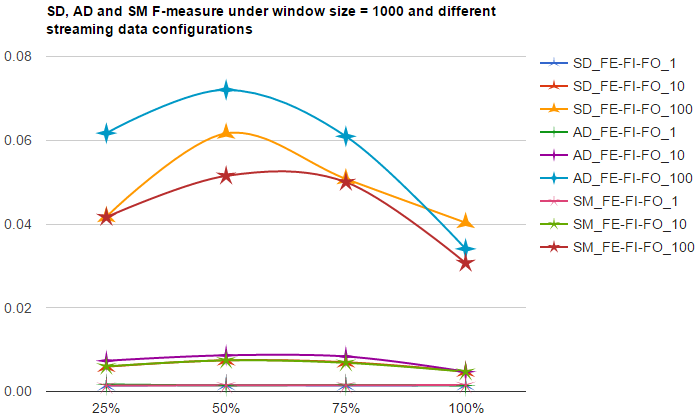
\includegraphics[width=5in]{img/4-ff.png}
	\caption{F-measure of Different Windows with FEFO}
	\label{fig:fefo}
\end{figure}

Figure \ref{fig:fefo} shows the F-measure performances brought by different windows. 
Some easy observations are: 
(1) the F-measure increases as the streaming throughput increases;
(2) the F-measure at $d = 50\%\ l$ is always best, and 100\% is always worst for all cases;
(3) AD\_FE-FI-FO performs similarly as others do when streaming throughput is 1 triple per graph, but outperforms as the streaming configuration increases;
(4) SD\_FE-FI-FO and SM\_FE-FI-FO compete with each other in each test run.

The above observations can partially answer the first question, with the points that different triple-store producers do affect the F-measure performance, but different window configurations do not have a significant influence. 
The greater the streaming input, the more influences are made on F-measure. 
However, in order to give a thorough answer we need to look at other metrics before assessing the overall performance. 
For example, AD\_FE-FI-FO gives the best F-measure, but does it take more time to execute the query and data eviction?

\begin{figure}[!htbp]
	\centering
	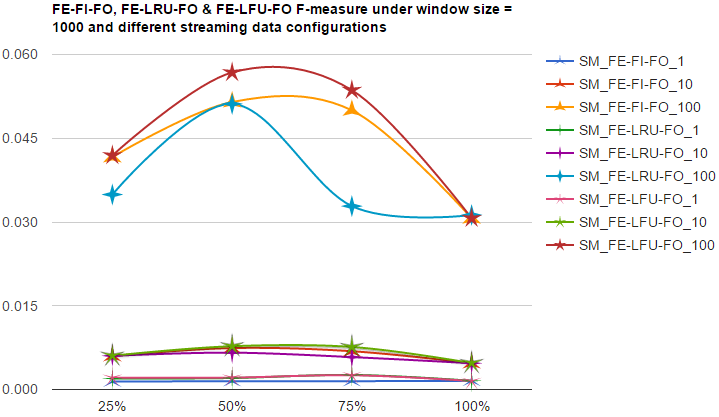
\includegraphics[width=5in]{img/4-fds.png}
	\caption{F-measure of SM Window with Different Strategies}
	\label{fig:diff}
\end{figure}

Figure \ref{fig:diff} shows the F-measure performance by different strategies for the SM windows with different streaming data configurations. 
The observations are: 
(1) F-measure increases as the streaming throughput increases;
(2) $d = 50\%\ l$ has the biggest F-measure score, 100\% has the smallest score for all the cases;
(3) for the same streaming data configuration, FE-LFU-FO always performs best, followed by FE-LRU-FO and then FE-FI-FO.

These observations can answer the second question from the perspective of big window size. 
Nevertheless, does window size affect these strategies' performances? 
Does it take longer time to explain all of the inferences? 
If yes, is it worthwhile to sacrifice system responsiveness for a better F-measure?

Additional observations are as follows:
(1) F-measure score: our raw experimental results have shown that F-measure increases as the window size increases. 
The F-measure score is also affected by different triple-stores. 
We believe this is because AlllegroGraph's and Stardog's inner implementation engines and mechanisms are different\footnote{Exploration and explanation of triple-stores' inner implementations are out of the scope of this dissertation}.    
(2) Memory consumption: when $l=10$, cases of $T_{pg}=1$ require 3 times on average the memory of bigger streaming configured cases. 
When $l=100$, the overall memory consumption decreases as the eviction amount (window step) increases. 
When $l=1000$, the overall memory consumption increases as the eviction amount (window step) increases. 
However, within this evaluation, no significant differences are observed between memory-based window and disk-based window. 
Small window and streaming throughput cases usually requires more memory.
Average FE-FI-FO strategy memory consumed is 41.93MB, FE-LRU-FO is 40.4MB and FE-LFU-FO is 39.59MB.
(3) Query time: AD requires the most query time for all cases. 
SD requires less time than AD but more than SM. 
The query time increases as window size and streaming input increases.
One potential reason for this is because a disk-based window needs some IO time when executing a query, which takes more time than a memory-based window. 
Average query time for all FE-FI-FO cases is 18ms, FE-LRU-FO is 15ms, FE-LFU-FO is 13ms.
(4) Explanation time: result explanation time increases approximately linearly as window and streaming input increases. 
In most cases, FE-LFU-FO takes longer time to explain.
Average FE-LFU-FO explanation time is 90371ms, FE-LRU-FO is 86100ms.
(5) Eviction time: eviction time increases as eviction amount, window size and streaming input increases. 
AD eviction time is very fast, 30ms on average. 
SD on average is 2879ms. 
SM on average is 4042ms.

According to the window and streaming data configurations, there can be either 10, 100, 1,000, 10,000 or 100,000 triples in the window during one processing loop. 
We identify a small case where 10 or 100 triples are processed, a medium case where 1,000 or 10,000 triples are processed, and a large case where 100,000 triples are processed. 
Together with Table \ref{tab:tradeoff}, we present a thorough comparison among triple-stores, window types and data management strategies under these scenarios, as well as to help answer the third question above-mentioned, i.e., what are the trade-offs to consider when deploying our architecture in different scenarios?

\begin{table*}[!htbp]
\centering
\caption{The Trade-off Table}
\label{tab:tradeoff}
\resizebox{\textwidth}{!}{%
\begin{tabular}{|c|c|l|r|r|r|r|r|}
\hline
Scenario & Tuple \# in window & window Config. & \multicolumn{1}{c|}{SPARQL (ms)} & \multicolumn{1}{c|}{F-measure} & \multicolumn{1}{c|}{Explain (ms)} & \multicolumn{1}{c|}{Eviction (ms)} & \multicolumn{1}{c|}{Memory (MB)} \\ \hline
\multirow{14}{*}{Small} & \multirow{7}{*}{10} &AllegroGraph& 20.25 & 4.35E-05 & - & 69.25 & 22.00 \\
&&Stardog& 5.13 & 3.93E-05 & - & 11.00 & 56.75 \\ \cline{3-8} 
&& Disk & 8.69 & 5.43E-05 & 1970.25 & 26.94 & 57.00 \\
&& Memory & 5.00 & 5.40E-05 & 1790.25 & 9.50 & 56.25 \\ \cline{3-8} 
&& FE-FI-FO & 10.17 & 4.07E-05 & 0 & 30.42 & 45.17 \\
&& FE-LRU-FO & 5.00 & 5.68E-05 & 1571.00 & 11.50 & 61.38 \\
&& FE-LFU-FO & 4.63 & 7.19E-05 & 2189.50 & 11.50 & 74.75 \\ \cline{2-8} 
& \multirow{7}{*}{100} &AllegroGraph& 11.63 & 2.97E-04 & - & 73.38 & 58.38 \\
&&Stardog& 5.00 & 3.05E-04 & - & 20.81 & 42.81 \\ \cline{3-8} 
&& Disk & 6.75 & 3.70E-04 & 8058.81 & 34.94 & 41.88 \\
&& Memory & 4.92 & 3.84E-04 & 8178.63 & 20.17 & 41.08 \\ \cline{3-8} 
&& FE-FI-FO & 5.41 & 2.27E-04 & 0 & 28.75 & 36.00 \\
&& FE-LRU-FO & 5.41 & 4.17E-04 & 7846.44 & 21.38 & 37.19 \\
&& FE-LFU-FO & 5.00 & 4.44E-04 & 8391.00 & 21.25 & 36.19 \\ \hline
\multirow{14}{*}{Medium} & \multirow{7}{*}{1,000} &AllegroGraph& 12.17 & 1.53E-03 & - & 89.42 & 59.08 \\
&&Stardog& 6.46 & 1.55E-03 & - & 164.96 & 36.21 \\ \cline{3-8} 
&& Disk & 8.35 & 1.68E-03 & 25372.54 & 129.35 & 40.52 \\
&& Memory & 6.56 & 1.74E-03 & 25265.42 & 169.14 & 36.97 \\ \cline{3-8} 
&& FE-FI-FO & 8.36 & 1.54E-03 & 0 & 139.78 & 43.53 \\
&& FE-LRU-FO & 6.96 & 1.82E-03 & 24355.21 & 151.33 & 37.54 \\
&& FE-LFU-FO & 7.04 & 1.85E-03 & 26282.75 & 151.42 & 33.21 \\ \cline{2-8} 
& \multirow{7}{*}{10,000} &AllegroGraph& 15.63 & 7.25E-03 & - & 90.00 & 33.38 \\
&&Stardog& 9.56 & 6.49E-03 & - & 1575.38 & 37.93 \\ \cline{3-8} 
&& Disk & 11.34 & 6.77E-03 & 122612.38 & 1020.72 & 39.41 \\
&& Memory & 9.22 & 6.77E-03 & 144213.08 & 1150.50 & 36.28 \\ \cline{3-8} 
&& FE-FI-FO & 11.58 & 6.75E-03 & 0 & 1080.25 & 36.42 \\
&& FE-LRU-FO & 9.50 & 6.18E-03 & 113897.38 & 1556.94 & 40.81 \\
&& FE-LFU-FO & 9.81 & 6.89E-03 & 113782.88 & 1004.19 & 32.13 \\ \hline
\multirow{7}{*}{Large} & \multirow{7}{*}{100,000} &AllegroGraph& 127.75 & 5.72E-02 & - & 187.25 & 23.50 \\
&&Stardog& 76.13 & 4.60E-02 & - & 27949.00 & 36.13 \\ \cline{3-8} 
&& Disk & 134.31 & 4.64E-02 & 261564.75 & 17122.81 & 31.13 \\
&& Memory & 15.17 & 4.22E-02 & 271454.38 & 32248.08 & 36.67 \\ \cline{3-8} 
&& FE-FI-FO & 93.33 & 4.97E-02 & 0 & 18695.08 & 31.92 \\
&& FE-LRU-FO & 84.88 & 3.57E-02 & 263054.63 & 27104.50 & 33.63 \\
&& FE-LFU-FO & 66.50 & 4.58E-02 & 269964.50 & 27470.63 & 35.75 \\ \hline
\end{tabular}
}
\end{table*}
Each value in the table is calculated from raw experimental results.
Please refer to our github repository for these raw results. 
In the 10 triples/window scenario, for example, 
disk-based window's F-measure score is averaged from AD\_FE-FI-FO, SD\_FE-FI-FO, SD\_FE-LRU-FO \& SD\_FE-LFU-FO test cases, 
while memory-based window's score is averaged from SM\_FE-FI-FO, SM\_FE-LRU-FO \& SM\_FE-LFU-FO test cases.
We would like to highlight an empirical comparison of the two window types, the disk-based window (DC) and the memory-based window (MC).

The detailed comparisons of all aspects for different scenarios are provided as follows:
(1) SPARQL query time: for every scenario, DC is slower than MC. 
As the scenario increases, DC grows much faster than MC. 
The ratio between 100,000 triples/window and 10 triples/window for DC is 15.45, whilst MC is 3.34. 
Though DC is less restricted by storage space, its query time slows down the system response time, and this effect will become worse as the scenario size grows.
However, this is expected, as accessing disk when executing query is always slower than accessing the memory.     
(2) F-measure: for every scenario, DC's and MC's F-measure scores are very similar. 
This means both types are able to provide same level correctness.
F-measure increases as scenario increases, this is because the more data in the window, the more correct results can be calculated, which raises the F-measure.	
(3) Reasoning Explanation Time: in most scenarios, MC's explanation time is slower than DC's. 
The difference increases significantly as the scenario size increases.
Reasoning explanation is very time-consuming. 
Strategies (such as FE-LFU-FO) requiring reasoning-explanation provide better F-measure when the scenario is small and explanation time is quick, but provide similar F-measure when the scenario is large and explanation time is slow.	
(4) Eviction Time: in small scenarios, DC is slower; in medium and large scenarios, MC is slower.
The difference between DC and MC increases significantly as the scenario size increases. 
This indicates a bias towards DC for large RDF streams, and MC for small RDF streams.	
(5) Memory Consumption: Both DC and MC consume similar memory for each scenario. 
This could be because Stardog triple-stores are implemented very efficiently, but again, explaining this requires the knowledge of inner mechanisms of Stardog, which is out of the scope of this work. 

Under the small case, AllegroGraph's query and eviction time is several times that of Stardog. 
Disk and memory performs equally on F-measure, though disk requires more time to query, evict and explain. 
FE-LFU-FO performs best in F-measure, followed by FE-LRU-FO then FEFO. 
Though FEFO needs more time to query and evict, the explanation time required by FE-LRU-FO and FE-LFU-FO is significantly greater. 
The trade-offs in deploying our framework under the small scenario is dependent on the use case. 
If system responsiveness is the first class citizen, a FEFO strategy will be chosen since it does not require explanation and provides a fine F-measure. 
Stardog memory window can be chosen since it provides faster execution time and better F-measure. 
If F-measure is most important, FE-LFU-FO is the right strategy.
Stardog memory window is the best as memory window provides less explanation time. 
It is also noticed that $d = $ 25\% or 50\% of $l$ provides better F-measure.

For medium cases, Stardog's eviction time increases significantly.
Though Stardog's query time is better than AllegroGraph's, the difference is very small when compared with the eviction time.
Disk window provides less eviction time; its other metrics are similar as memory windows.
FE-LFU-FO is the best at F-measure scores, but is traded for longer explanation time.
Actually FEFO provides decent F-measure without explanation time.
Overall, AllegroGraph disk window with FEFO is most suitable for this scenario.
$d=50\%$ or $75\%$ of $l$ provides best F-measure as well.

For large cases, AllegroGraph's eviction time, F-measure and memory performs better, though query is slower.
Disk window query time is 9 times greater than the memory dependent graph database, but provides better F-measure, explanation , eviction time and memory. 
FEFO performs best in F-measure but it spends more time on query, with smallest eviction time and memory consumption. 
Hence, AllegroGraph disk window with FEFO is most suitable for this experiment's use case. It is also recommended to use $d = 50\% $ of $l$ to provide the best F-measure.
%
\section{Summary}
This chapter introduces the sequential stream reasoning architecture, and shows how semantic importance model can be used in stream reasoning applications. 
The window is implemented with two off-the-shelf triple-stores (Stardog or AllegroGraph), with different configurations (memory-based or disk-based).
The benchmark leverages LUBM dataset by streaming it, and constantly looking for the answers of the query ``who is a professor?'', which requires RDFS reasoning.
This can be seen to look for professors on a time line by streaming the LUBM dataset. 
In order to illustrate how to use semantic importance in stream reasoning with SSRA, four aspects $\tau_{a}$, $\tau_{e}$, $f_{qp}$ and $\tau_{qp}$ are chosen to form three window management strategies:
FE-FI-FO with its priority vector $[\tau_{a}, \tau_{e}]$, FE-LFU-FO with $[\tau_{e}, f_{qp}, \tau_{a}]$, and FE-LRU-FO with $[\tau_{e}, \tau_{qp}, \tau_{a}]$. 
The SSRA implementations have demonstrate a physical sliding window, but the temporal window is easy to implement as well according to the extended window semantics.
The architecture operational semantics is very flexible, as the data consumption component is able to realize different operational semantics. 
In all three implementations, the report policy is ``on window close''.
The continuous processing is enabled by the inner loop of the architecture. 
The query is a pure SPARQL query, which is different from most of the existing work. 
The window is implemented in the triple-store, with a graph ID manager that indexes graph IDs, and updates data semantic importance priority vectors.
The benchmark results show that the architecture is scalable, but for strategies involved with query participation aspects, as the window size increases, the result explanation time increases significantly.
Thus, in order to use query participation aspect, the window size has either to be kept relatively small, which is one of the incentives that semantic importance is proposed, 
or to use some filtering functionality such as query relevance aspect in the semantic importance model in order to reduce the data in the window. 
In the next chapter, we will show how to keep the window size small with the architecture and semantic importance, as well as show how the proposed model and infrastructure can be leveraged for real-life use cases.
%%%%%%%%%%%%%%%%%%%%%%%%%%%%%%%%%%%%%%%%%%%%%%%%%%%%%%%%%%%%%%%%%%%% 
%                                                                 %
%                            CHAPTER Four                         %
%                                                                 %
%%%%%%%%%%%%%%%%%%%%%%%%%%%%%%%%%%%%%%%%%%%%%%%%%%%%%%%%%%%%%%%%%%% 

\chapter{USE CASES}
In this chapter, two use cases are implemented based on semantic importance and the sequential stream reasoning architecture.
The use cases leverage different combinations of semantic importance aspects which support different window management strategies.
This chapter aims to show how semantic importance is determined, deployed in stream reasoning use cases, as well as how semantic importance impacts the system performance. 
%
\section{Soccer Offside Detection}
This use case detects soccer offside offence with a particular focus on the accuracy, error and running performance of window management strategies based on the semantic importance.
%
\subsection{Background}
Soccer (a.k.a. association football) is one of the most influential and competitive sports across the globe. 
In soccer games, one common offence among others is called ``offside offence''. 
FIFA\footnote{\url{https://www.fifa.com/}} defines it in a comprehensive way.
For details, please refer to Rule 11 in FIFA laws of the game \cite{federation2016laws}.
However, it is worth to mention a key point: that a player is at an offside position is determined at the moment when the ball is played by this player's teammate; once identified, this status will be retained until the ball is touched again. 
For example, when Player A2 passes the ball to his teammate Player A1 who is at an offside position, even if Player A1 relocates himself to touch the ball in an onside position, it is still considered as an offside offence. 

In order to give accurate offside decisions, a linesman (assistant referee) in his/her assigned half field needs to keep close track of the second-last defender, the ball-passing moment and any attackers at the offside position.
However, the fast tempo and heated atmosphere of the soccer game, together with linesmen' limited visual field and potential tiredness, can contribute to erroneous offside judgments, which may allow illegal attacking opportunities or disallow legal ones, and consequently affect the outcome of the game.

A number of studies have focused on the prevalence of offside mistakes by linesmen. 
\cite{catteeuw2010offside} investigates the accuracy of offside judgments in the English Premier League, with a reported error rate of 17.5\%. This is possibly because the English linesmen tend not to signal in doubtful situations, so there is an overall bias towards non-flag errors (773 non-flag errors vs 95 flag errors).
Another study \cite{helsen2006errors} analyzes 337 offside judgments in all 64 games during the 2002 FIFA World Cup, and finds the error percentage to be 26.2\%.
\cite{catteeuw2010offside} also examines the accuracy of offside judgments during the 2006 FIFA World Cup, and finds an error rate of 7.6\%, significantly lower than that of \cite{helsen2006errors}.
This study argues that the reduction in error rate might be due to different approaches the authors take to count errors.
The study also reveals higher rate of non-flag errors (9.6\%) than flag errors (6.9\%), within the overall error rate of 7.6\%.

A 2013 report \cite{fowler2010feasible} analyzes several offside detection systems, and proposes a number of evaluation criterion such as accuracy, fairness, system delays, feasibility, cost and intrusiveness of the system development and deployment.
Offside event detection methods may be based on various technologies, such as image processing \& computer vision \cite{naidoo2006soccer}, and stereo vision tracking  \cite{borg2007detecting}.
In addition to vision-based tools, sensor-enabled equipment is also employed in this scenario \cite{regan2013sports} \cite{garcia2011wireless}.
An example is the sports vest provided by GPsports\footnote{\url{http://gpsports.com/}}, which has been already used in the professional soccer.
The GPsports vest is equipped with sensors that track volume, intensity and work rate of matches played or training by recording and analyzing real-time data such as player position, velocity and heart rate.
According to its official website, this system has been successfully adopted by 150 clients of 10 sports, including prestigious soccer teams such as Real Madrid C.F. and Chelsea F.C.

Overall, sensor-based systems have great advantages by providing real-time, high-frequency, high-speed motion data of all available participants, but they lack the ability to determine the precise positions of players with reference to relevant boundaries required for offside calculations. 
Vision-based technologies are getting more precise for player boundary proximity detection, but output credibility and cost of computation have been major concerns.

The fact that gears like the GPsports vest have become more pervasive provides both opportunities and challenges for soccer. 
The opportunities lie in analysis of the real-time streaming data for players' kinetic and biological statistics such as location, velocity, acceleration, heart rate, breathing, and so forth. 
The challenges also come with the data: these systems require technologies to efficiently process constantly-updating, high volume and heterogeneous real-time streaming data in order to better analyze player performance for coaches, provide timely input of relevant officiating content for referees, and help spectators to enjoy the match. 
While contemporary stream processing systems are able to store and query low-level data at high speed, they do not typically have a framework to also furnish higher-level information that is implicit in the data.  
This is because this implicit information (e.g. player tiredness, opponent strategy, etc.) is not directly revealed by a stream processing system, which can only process explicit data (e.g. player position, velocity) and support window-based queries.  
In a soccer scenario, for example, a pure stream processing system would not be able to tell the coach that his left fullback is becoming tired and could be exploited by the opponent's fast right winger, or make other tactical suggestions. 
%
\subsection{Approach}
Timestamp metadata, such as arrival timestamp, has each been investigated as a key feature for window management.
But it only scratches the surface of possible ways to establish a specific window management strategy. 
Overall, a good window management strategy implementation will look for the right combination of heuristic guidelines that best capture the important information for the queries at hand.
In considering these heuristics, there are certain domain-independent contributors (e.g. time and use frequency), but there are also domain-dependent contributors that stem from the requirements of the particular use case, such as the goal of the use case, the specific answers expected from the data, the background knowledge and constraints, specific space and time limitations, etc. 
Knowing these requirements, humans can often determine efficient policies about which data will contribute to the query. 
For example, because we know that only an attacker can commit an offside offence, we can conclude that positional data for the defenders will never contribute to the query, and so is unimportant and can be flushed from the window.  
%
\subsection{Date Stream}
The data was collected during a practice game played on a half-sized soccer field. 
It includes information for one referee, two teams, eight players (including one goalkeeper) per team, and four balls (one ball is in play while the other three are backup balls). 
Sensors, installed in the center of the balls, and on the shin-guards and gloves of the players and referees, constantly stream kinetic data at high frequencies, such as position, velocity, acceleration, and directional vector. 
The ball sensor is 2000Hz, the player/referee sensor is 200Hz.
For more details, please refer to \cite{mutschler2013debs}.

The game duration is two halves of thirty minutes each.
In addition to the streaming data, a full video of the game is provided. 
This use case hires a soccer referee certified by United States Soccer Association and National Intercollegiate Soccer Officials Association as a domain expert.
He reviewed the game video and provided a list of suggested officiating decisions for a total of twenty relevant scenarios, where decisions are given as ``offside offence'', ``no offence'', or ``unsure''.
His decisions are used as a ground truth to evaluate system precision.
%
\subsection{Ontology}
For this use case, the overall ontologies are modularized into three sub-ontologies:
(1) the individual ontology that encodes the specific match information such as teams and players in each team;
(2) the offside offence ontology that concentrates on the offside offence detection from the streaming data;
(3) the query relevance ontology that focuses on filtering out offside-irrelevant data from the streaming data.

\begin{figure}[!htbp]
	\centering
	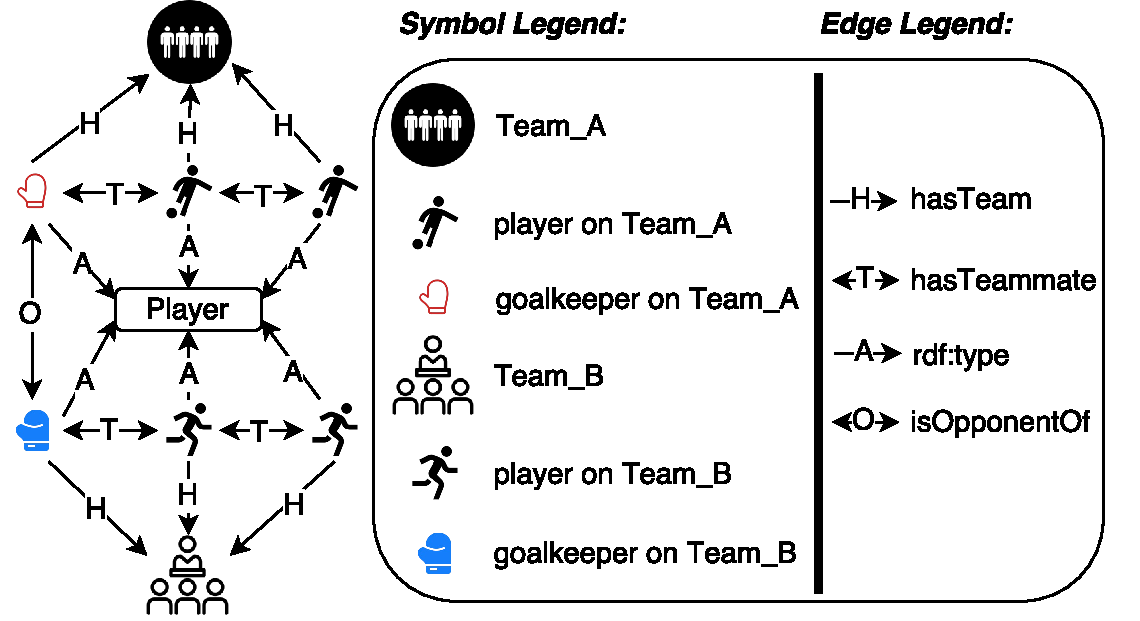
\includegraphics[width=5in]{img/5-matchOnto}
	\caption{Individual Ontology}
	\label{fig:matchOnto}
\end{figure}

For the purpose of illustration, three players are drawn from each team in Figure \ref{fig:matchOnto}.
All of the player individuals have a type of \textbf{Player}, which is a concept in the offside offence ontology.
\textit{hasTeam} is a functional property with a domain of \textbf{Player} and a range of \textbf{Team}.
Both \textit{hasTeammate} and \textit{isOpponentOf} are symmetric properties with \textbf{Player} as their domain and range.
\textit{hasTeammate} is transitive, meaning that a player can be his own teammate.\footnote{This is a modeling choice, not an error.}
\textit{isOpponentOf} is encoded only between two goalkeepers.

\begin{figure}[!htbp]
	\centering
	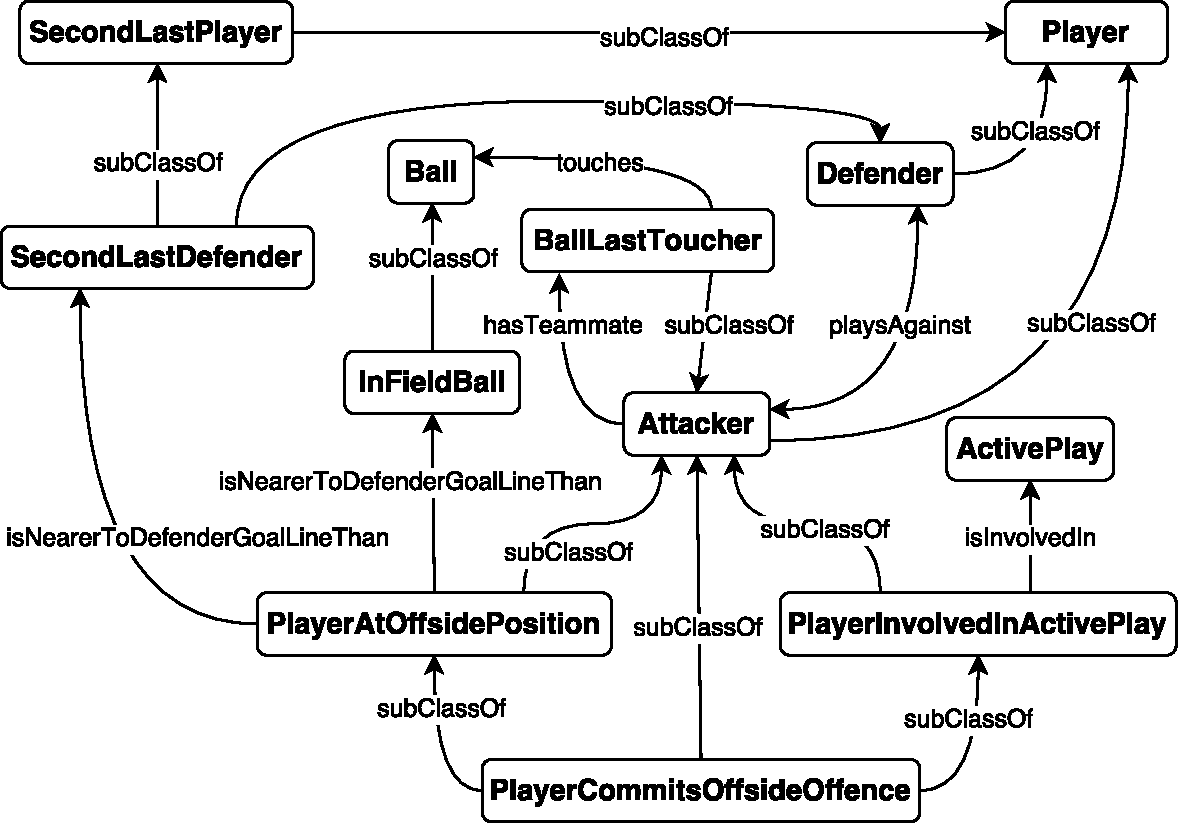
\includegraphics[width=5in]{img/5-soccerOnto}%
	\caption{Offside Offence Background Domain Ontology}
	\label{fig:soccerOnto}
\end{figure}

Figure \ref{fig:soccerOnto} shows the major classes and relations in order to describe the concept of the offside offence.
When developing this ontology, FIFA laws of the game \cite{federation2016laws} is used as the text corpus to extract a list of the offside relevant terms.
The term list was then carefully examined and curated to create a conceptual model, which was refined and extended to create the offside offence ontology\footnote{For more details, please refer to \url{https://tw.rpi.edu/web/Courses/Ontologies/2016/projects/soccer}}.
In a soccer game, usually the player who is touching the ball is considered to be an attacker, along with his teammates.
The concept to describe a player touching the ball is modeled as \textbf{BallLastToucher}, and the attackers as \textbf{Attacker}. 
An \textbf{Attacker} instance can either be the type of \textbf{BallLastToucher} or (\textit{hasTeammate some} \textbf{BallLastToucher}).
\textbf{Defender} is defined as (\textbf{Player} \textit{and} (\textit{playsAgainst some} \textbf{Attacker})),
where \textit{playsAgainst} is a symmetric property chain as (\textit{isOpponentOf o hasTeammate}).
Instead of manually labeling play-against relationship for each pair of opponent players, leveraging this property chain and a reasoner, \textit{playsAgainst} is automatically established.
This saves lots of tedious work, keeps a compact ontology, and shows the value of the semantics.
\textbf{SecondLastDefender} is one of the key concepts to define the soccer offside.
It is the subclass of both \textbf{SecondLastPlayer} and \textbf{Defender}.
We directly annotate a player as \textbf{SecondLastPlayer} for each team by selecting the player who is the second-nearest to his own goal line among his team. 
This is to reflect the real world scenario that the linesman should always keep up with the second last player of his assigned half.
The ball being played is an \textbf{InFieldBall}, whereas the other balls are \textbf{BackupBall}.
When a player is classified as an \textbf{Attacker}, and \textit{isNearerToDefenderGoalLineThan} both \textbf{SecondLastDefender} and \textbf{InFieldBall}, then he/she is further classified as \textbf{PlayerInOffsidePosition}.
If a player touches the ball or challenges an opponent, he/she is classified as \textbf{PlayerInvolvedInActivePlay}.
According to the symplified definition of the soccer offside offence in Chapter 1, when a player is classified as both \textbf{PlayerInOffsidePosition} and \textbf{PlayerInvolvedInActivePlay}, he/she, who is therefore classified as \textbf{PlayerCommitsOffsideOffence}, commits an offside offence.

\begin{figure}[!htbp]
	\centering
	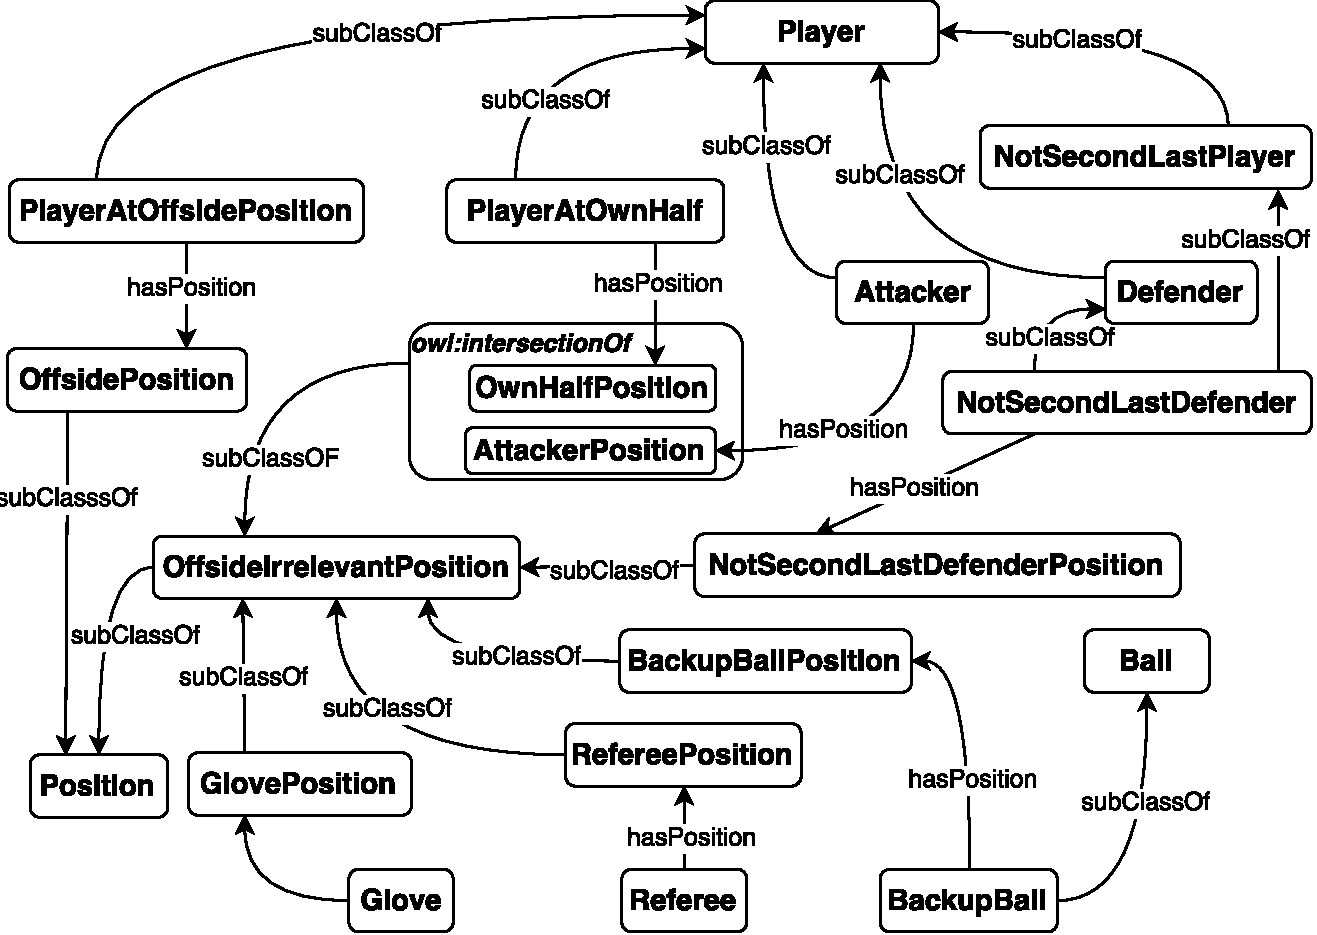
\includegraphics[width=5in]{img/5-qronto}
	\caption{Soccer Offence Query Relevance Ontology}
	\label{fig:dlonto}
\end{figure}

Figure \ref{fig:dlonto} illustrates the query relevance ontology. 
This use case is scoped to answer the question of who commits an offside offence. 
If a data item does not contain offside offence information, there is no need to execute the query on it. 
The purpose of this ontology module is to identify and eliminate the irrelevant data by leveraging semantics to ask another question (an example is in Listing 5.2) of what the offside irrelevant positions are prior to executing the offside query.
For the data set of this use case, all ball positions, referee positions, goalkeeper glove positions and player's positions are present. 
In this ontology, glove's position \textbf{GlovePosition}, referee's position \textbf{RefereePosition}, back up balls' positions \textbf{BackupBallPosition}, positions of defenders who are not the second last player \textbf{NotSecondLastDefenderPosition}, positions of attackers who are in their own half (\textit{owl:intersectionOf} (\textbf{AttackerPosition} \textit{and} \textbf{OwnHalfPosition})) are all offside irrelevant positions \textbf{OffsideIrrelevantPosition}, which means that these types of data will not provide necessary information to the query at hand, thus can be filtered out before the target query execution. 
%
\subsection{Data Annotation}
The original streaming data comes in comma-delimited format with the schema as  ($sid, ts, x, y, z, \left|v\right|, \left|a\right|, v_{x}, v_{y}, v_{z}, a_{x}, a_{y}, a_{z}$), where $sid$ denotes the sensor ID, $ts$ denotes the generation timestamp in pico-seconds, $(x, y, z)$ denotes a sensor coordinate in 3D space, and $(\left|v\right|, \left|a\right|, v_{x}, v_{y}, v_{z}, a_{x}, a_{y}, a_{z})$ denotes sensor velocity, acceleration and their directions.
In this use case, $(sid, ts, x, y, z)$ will be used.

Each shin-guard of a player is installed with a sensor.
A player's position is obtained by averaging his sensor coordinates.
With the coordinates of the field markings, and player/ball positions, position coordinates can be calculated to get information, such as which balls are on or off the field or which players are in or not in their own half, etc. 
Euclidean distance is used to determine if there is an active play of either a ball-touch or an opponent-challenge.
All players are ranked according to their distances from the ball in play.
The Player-ball distance is not based on the averaged player coordinate, but the actual left and right shinguard sensor to ball sensor. 
This increases the annotation accuracy. 
That a player touches the ball is determined when he has the nearest distance to the ball that is less than 0.6 meter.
An opponent-challenge scenario is also determined when opponent-opponent distance is less than 0.6 meter.
Once a ball-touch is detected, all attacking players' distance from the defender goal line and the ball will be calculated.
Each player's distance from his own goal line will also be calculated so as to determine who is the second-last player of each team. 
The data is then annotated as in Table \ref{tab:dat}.

\begin{table}[!htbp]
    \centering
	\caption{Data Annotation Table}
    \label{tab:dat}
    \begin{tabular}{|c|c|} \hline
        data & annotation \\ \hhline{|==|}
		\multicolumn{2}{|c|}{player annotation} \\ \hhline{|==|}
        \textit{playerX} position & \textit{:playerX :hasPosition :playerPosition\_ts} \\ \hline
        \textit{playerX} is in own half & \textit{:playerX a :PlayerInOwnHalf} \\ \hline
        \textit{playerX} is not in own half & \textit{:playerX a PlayerNotInOwnHalf} \\ \hline
        \textit{playerX} is a second-last player & \textit{:playerX a SecondLastPlayer} \\ \hline
        \textit{playerX} is not a second-last player & \textit{:playerX a NotSecondLastPlayer} \\ \hline
        \textit{playerX} touches the ball & \textit{:playerX :isInvolvedIn :ball\_touch} \\ \hline
        \multirow{2}{*}{if \textit{playerX} challenges \textit{playerY}} & \textit{:playerX :isInvolvedIn :opponent\_challenge} \\ & \textit{:playerY :isInvolvedIn :opponent\_challenge} \\ \hhline{|==|}
        \multicolumn{2}{|c|}{ball annotation} \\ \hhline{|==|}
        \textit{ballA} position & \textit{:ballA :hasPosition :ballPosition\_ts} \\ \hline
        \textit{ballA} is in the field & \textit{:ballA a :InFieldBall} \\ \hline
        \textit{ballA} is off the field & \textit{:ballA a :BackupBall} \\ \hhline{|==|}
        \multicolumn{2}{|c|}{referee \& glove annotation} \\ \hhline{|==|}
        referee position & \textit{:referee :hasPosition :refereePosition\_ts} \\ \hline
        glove position & \textit{:glove :hasPosition :glovePosition\_ts} \\ \hline
	\end{tabular}
\end{table}

%
\subsection{System Implementation}
The detection system is implemented with SSRA, where a SPARQL query in Listing 5.1 is deployed.
This query is simple, but requires Description Logic (DL) reasoning. 

\begin{lstlisting}[language=SPARQL,caption={Offside Offence Detection Query},basicstyle=\small,frame=single]
PREFIX so:<http://tw.rpi.edu/Ontologies/2016/Soccer_Offside/>
SELECT ?player 
WHERE { ?player a so:PlayerCommitsOffsideOffence.}
\end{lstlisting}

The data is sampled so that the balls' data update frequency is 20Hz, and the players' data update frequency is 10Hz.
Sampling will not affect the result as both balls and players move only a short distance every 0.05 and 0.1 second.

A physical sliding window is leveraged.
According to our annotation strategy, the maximum number of unique triples is 70, which includes the ``\textit{hasPosition}'' triples from 1 referee, 16 players, 4 balls and 4 gloves, as well as a certain number of ball status triples, such as ``\textit{ball4 a InFieldBall(BackupBall)}'', and player status triples, such as ``\textit{playerA4 a SecondLastPlayer(NotSecondLastPlayer, PlayerInOwnHalf, PlayerNotInOwnHalf)}'', ``\textit{playerA4 isInvolvedIn ball\_touch(opponent\_challenge)}'', etc. 
Thus the maximum physical window size ($l_{max}$) is set to be 70.

\begin{table}[!htbp]
\centering
\caption{Strategy Table}
\label{tab:sct}
\begin{tabular}{|l|c|}
\hline
\multicolumn{1}{|c|}{strategy} & semantic importance priority vector \\ \hline
FE-FI-FO & $[\tau_{e}, \tau_{a}]$ \\ \hline
FE-FI-FO-25\% & $[\tau_{e}, \tau_{a}]$ \\ \hline
FE-FI-FO-50\% & $[\tau_{e}, \tau_{a}]$ \\ \hline
FE-FI-FO-75\% & $[\tau_{e}, \tau_{a}]$ \\ \hline
QR-FE-FI-FO & $[qrf, \tau_{e}, \tau_{a}]$ \\ \hline
QR-FE-FI-FO-25\% & $[qrf, \tau_{e}, \tau_{a}]$ \\ \hline
QR-FE-FI-FO-50\% & $[qrf, \tau_{e}, \tau_{a}]$ \\ \hline
QR-FE-FI-FO-75\% & $[qrf, \tau_{e}, \tau_{a}]$ \\ \hline
FE-LFU-FO & $[\tau_{e}, f_{qp}]$ \\ \hline
FE-LFU-FO-25\% & $[\tau_{e}, f_{qp}]$ \\ \hline
FE-LFU-FO-50\% & $[\tau_{e}, f_{qp}]$ \\ \hline
FE-LFU-FO-75\% & $[\tau_{e}, f_{qp}]$ \\ \hline
QR-FE-LFU-FO & $[qrf, \tau_{e}, f_{qp}]$ \\ \hline
QR-FE-LFU-FO-25\% & $[qrf, \tau_{e}, f_{qp}]$ \\ \hline
QR-FE-LFU-FO-50\% & $[qrf, \tau_{e}, f_{qp}]$ \\ \hline
QR-FE-LFU-FO-75\% & $[qrf, \tau_{e}, f_{qp}]$ \\ \hline
FE-LRU-FO & $[\tau_{e}, \tau_{qp}]$ \\ \hline
FE-LRU-FO-25\% & $[\tau_{e}, \tau_{qp}]$ \\ \hline
FE-LRU-FO-50\% & $[\tau_{e}, \tau_{qp}]$ \\ \hline
FE-LRU-FO-75\% & $[\tau_{e}, \tau_{qp}]$ \\ \hline
QR-FE-LRU-FO & $[qrf, \tau_{e}, f_{qp}]$ \\ \hline
QR-FE-LRU-FO-25\% & $[qrf, \tau_{e}, f_{qp}]$ \\ \hline
QR-FE-LRU-FO-50\% & $[qrf, \tau_{e}, f_{qp}]$ \\ \hline
QR-FE-LRU-FO-75\% & $[qrf, \tau_{e}, f_{qp}]$ \\ \hline
\end{tabular}
\end{table}

For this use case, semantic importance aspects including $\tau_{a}$, $\tau_{e}$, $qrf$, $f_{qp}$, and $\tau_{qp}$ are chosen to form the strategies shown in Table \ref{tab:sct}. 
All strategies labeled with QR perform query relevance filtering (Listing 5.2) before executing the offside query in Listing 5.1. 
The percentage after each strategy indicates the percentage of $l_{max}$. 
For example, FE-LFU-FO-25\% means FE-LFU-FO strategy is performed in a window with 25\% of $l_{max}$, which is 70 $\times$ 0.25 = 17 data items.

This use case uses a different report policy that is not included in the SECRET model \cite{botan2010secret}.
It is named as ``on user-specified condition''. 
Specifically, the offside query is fired whenever a different player touches the ball.
It is important for this use case to execute the query based on ball touches, as all the status of the players will likely be changed upon each ball touch. 
Executing query based on time will potentially allow inconsistent data items, such as a player is both an attacker and defender. 

\begin{figure}[!htbp]
	\centering
	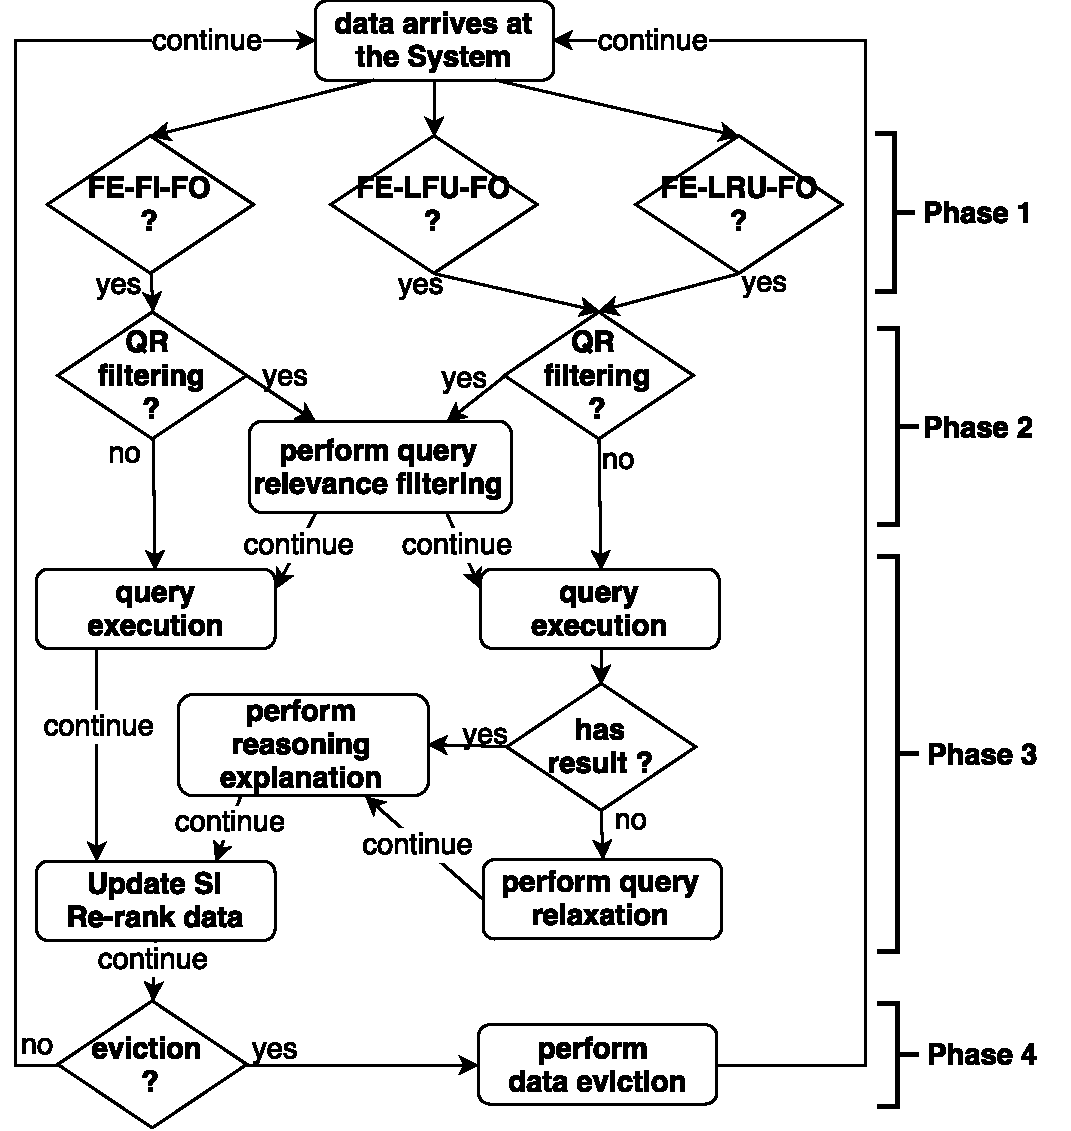
\includegraphics[width=5in]{img/5-strategyexe.pdf}
	\caption{Strategy Execution Flowchart}
	\label{fig:strExe}
\end{figure}

The strategies executed are shown by the paths through the graph in Figure \ref{fig:strExe}. 
Depending on the priority vector, Phase 1 is the selection of a base strategy family to run. 
If the SI priority vector has the first element of ``$qrf$'', the QR filtering is performed by executing the query in Listing 5.2.

\begin{lstlisting}[language=SPARQL,caption={Query Relevance Filtering Query},basicstyle=\small,frame=single]
PREFIX so:<http://tw.rpi.edu/Ontologies/2016/Soccer_Offside/>
SELECT ?player 
WHERE { ?position a so:OffsideIrrevelantPosition. }
\end{lstlisting}

Phase 3 executes the offside query when a new player touches the ball.
If current strategy is in the *-FI-FO family, the system will go ahead to update the semantic importance and re-rank the data. 
If the current strategy is in the *-LRU/LFU-FO family, the system will need to check if the offside query returns any results.
If there are results, reasoning explanation is performed to track all the triples that contribute to the query.
If no result, schema-aware query relaxation \cite{hurtado2008query} will be performed to increase the scope of the query.
For example, if the query returns no answer, the system continues to ask who touches the ball, who is the second-last player, who is nearer to the opponents' goal line than whom, etc. 
Listing 5.3 shows a relaxed query.

\begin{lstlisting}[language=SPARQL,caption={A Relaxed Query Example},basicstyle=\small,frame=single]
PREFIX so:<http://tw.rpi.edu/Ontologies/2016/Soccer_Offside/>
SELECT ?s ?p ?o
WHERE {
	?s a so:SecondLastPlayer.
	bind(IRI(rdf:type) as ?p).
	bind(IRI(so:SecondLastPlayer) as ?o)
}
\end{lstlisting}

Being able to preserve some partial necessary data and wait until the others arrive, and then answer the query, is a key feature for *-LRU/LFU-FO families enabled by $\tau_{qp}$ and $f_{qp}$.
It also explains why they have higher accuracy -- the offside offence judgement requires the window to preserve earlier information (player in offside position at the moment his teammate passes the ball) until later information (the player involved in an active play) arrives.
After query relaxation, semantic importance priority vectors will be updated, and the window data will be re-ranked. 
Next, the system checks the percentage of $l_{max}$ which the strategy comes with, and performs data eviction accordingly. 
Obviously, the use case expects that FE-FI-FO, QR-FE-FI-FO, FE-LFU-FO, QR-FE-LFU-FO, FE-LRU-FO and QR-FE-LRU-FO with $l_{max}$ will perform equally well in accuracy. 
%
\subsection{Evaluation}
Table \ref{tab:ev} presents both the referee and system offside judging results.
Table \ref{tb:rp} and \ref{tb:accuracy} show the averaged running performance and accuracy for each strategy family, respectively.  
Accuracy is computed by counting a correct answer only when referee gives \textcolor{blue}{\newmoon} and system gives \newmoon, or when referee gives \textcolor{blue}{\texttimes} and system gives \texttimes. 
For example, we calculate FE-FI-FO-25\% accuracy as 11/20 = 0.55 because it gives 11 correct results out of the total 20 cases.

\begin{table}[!htbp]
	\scriptsize
	\centering
	\caption{Offside Detection Results}
	\label{tab:ev}
	\begin{tabular}{|l|c|c|c|c|c|c|c|c|c|c|} \hline
Time&2:53&4:26&7:04&12:21&12:44&15:28&20:40&21:11&22:07&23:04\\ \hhline{|=|=|=|=|=|=|=|=|=|=|=|}
\textcolor{blue}{Referee}&\textcolor{blue}{\texttimes}&\textcolor{blue}{\newmoon}&\textcolor{blue}{\newmoon}&\textcolor{blue}{\texttimes}&\textcolor{blue}{\texttimes}&\textcolor{blue}{\newmoon}&\textcolor{blue}{\newmoon}&\textcolor{blue}{\newmoon}&\textcolor{blue}{\texttimes}&\textcolor{blue}{\texttimes}\\ \hline
FE-FI-FO&\texttimes&\newmoon&\newmoon&\texttimes&\texttimes&\newmoon&\newmoon&\textcolor{red}{\texttimes}&\texttimes&\texttimes\\ \hline
FE-FI-FO-25\%&\texttimes&\textcolor{red}{\fullmoon}&\textcolor{red}{\texttimes}&\textcolor{red}{\newmoon}&\texttimes&\textcolor{red}{\fullmoon}&\textcolor{red}{\texttimes}&\textcolor{red}{\fullmoon}&\texttimes&\texttimes\\ \hline
FE-FI-FO-50\%&\texttimes&\textcolor{red}{\texttimes}&\textcolor{red}{\texttimes}&\textcolor{red}{\newmoon}&\texttimes&\textcolor{red}{\texttimes}&\textcolor{red}{\texttimes}&\textcolor{red}{\texttimes}&\texttimes&\texttimes\\ \hline
FE-FI-FO-75\%&\texttimes&\textcolor{red}{\texttimes}&\textcolor{red}{\texttimes}&\texttimes&\texttimes&\textcolor{red}{\texttimes}&\textcolor{red}{\texttimes}&\textcolor{red}{\texttimes}&\texttimes&\texttimes\\ \hline
QR-FE-FI-FO&\texttimes&\newmoon&\newmoon&\texttimes&\texttimes&\newmoon&\newmoon&\textcolor{red}{\texttimes}&\texttimes&\texttimes\\ \hline
QR-FE-FI-FO-25\%&\texttimes&\textcolor{red}{\fullmoon}&\textcolor{red}{\texttimes}&\textcolor{red}{\newmoon}&\texttimes&\textcolor{red}{\fullmoon}&\textcolor{red}{\texttimes}&\textcolor{red}{\fullmoon}&\texttimes&\texttimes\\ \hline
QR-FE-FI-FO-50\%&\texttimes&\textcolor{red}{\texttimes}&\textcolor{red}{\texttimes}&\textcolor{red}{\newmoon}&\texttimes&\textcolor{red}{\texttimes}&\textcolor{red}{\texttimes}&\textcolor{red}{\texttimes}&\texttimes&\texttimes\\ \hline
QR-FE-FI-FO-75\%&\texttimes&\textcolor{red}{\texttimes}&\textcolor{red}{\texttimes}&\texttimes&\texttimes&\textcolor{red}{\texttimes}&\textcolor{red}{\texttimes}&\textcolor{red}{\texttimes}&\texttimes&\texttimes\\ \hline
FE-LFU-FO&\texttimes&\newmoon&\newmoon&\texttimes&\texttimes&\newmoon&\newmoon&\textcolor{red}{\texttimes}&\texttimes&\texttimes\\ \hline
FE-LFU-FO-25\%&\texttimes&\newmoon&\newmoon&\texttimes&\texttimes&\newmoon&\newmoon&\textcolor{red}{\fullmoon}&\texttimes&\texttimes\\ \hline
FE-LFU-FO-50\%&\texttimes&\newmoon&\newmoon&\texttimes&\texttimes&\newmoon&\newmoon&\textcolor{red}{\fullmoon}&\texttimes&\texttimes\\ \hline
FE-LFU-FO-75\%&\texttimes&\newmoon&\newmoon&\texttimes&\texttimes&\newmoon&\newmoon&\textcolor{red}{\texttimes}&\texttimes&\texttimes\\ \hline
QR-FE-LFU-FO&\texttimes&\newmoon&\newmoon&\texttimes&\texttimes&\newmoon&\newmoon&\textcolor{red}{\texttimes}&\texttimes&\texttimes\\ \hline
QR-FE-LFU-FO-25\%&\texttimes&\newmoon&\newmoon&\texttimes&\texttimes&\newmoon&\newmoon&\textcolor{red}{\fullmoon}&\texttimes&\texttimes\\ \hline
QR-FE-LFU-FO-50\%&\texttimes&\newmoon&\newmoon&\texttimes&\texttimes&\newmoon&\newmoon&\textcolor{red}{\fullmoon}&\texttimes&\texttimes\\ \hline
QR-FE-LFU-FO-75\%&\texttimes&\newmoon&\newmoon&\texttimes&\texttimes&\newmoon&\newmoon&\textcolor{red}{\fullmoon}&\texttimes&\texttimes\\ \hline
FE-LRU-FO&\texttimes&\newmoon&\newmoon&\texttimes&\texttimes&\newmoon&\newmoon&\textcolor{red}{\texttimes}&\texttimes&\texttimes\\ \hline
FE-LRU-FO-25\%&\texttimes&\newmoon&\newmoon&\texttimes&\texttimes&\newmoon&\newmoon&\textcolor{red}{\fullmoon}&\texttimes&\texttimes\\ \hline
FE-LRU-FO-50\%&\texttimes&\newmoon&\newmoon&\texttimes&\texttimes&\newmoon&\newmoon&\textcolor{red}{\fullmoon}&\texttimes&\texttimes\\ \hline
FE-LRU-FO-75\%&\texttimes&\newmoon&\newmoon&\texttimes&\texttimes&\newmoon&\newmoon&\textcolor{red}{\fullmoon}&\texttimes&\texttimes\\ \hline
QR-FE-LRU-FO&\texttimes&\newmoon&\newmoon&\texttimes&\texttimes&\newmoon&\newmoon&\textcolor{red}{\texttimes}&\texttimes&\texttimes\\ \hline
QR-FE-LRU-FO-25\%&\texttimes&\newmoon&\newmoon&\texttimes&\texttimes&\newmoon&\newmoon&\textcolor{red}{\fullmoon}&\texttimes&\texttimes\\ \hline
QR-FE-LRU-FO-50\%&\texttimes&\newmoon&\newmoon&\texttimes&\texttimes&\newmoon&\newmoon&\textcolor{red}{\fullmoon}&\texttimes&\texttimes\\ \hline
QR-FE-LRU-FO-75\%&\texttimes&\newmoon&\newmoon&\texttimes&\texttimes&\newmoon&\newmoon&\textcolor{red}{\fullmoon}&\texttimes&\texttimes\\ \hhline{===========}
Time&30:52&40:30&40:45&42:16&47:38&50:25&51:43&54:46&58:11&58:24 \\  \hhline{|=|=|=|=|=|=|=|=|=|=|=|}
\textcolor{blue}{Referee}&\textcolor{blue}{\texttimes}&\textcolor{blue}{\texttimes}&\textcolor{blue}{\newmoon}&\textcolor{blue}{$\otimes$}&\textcolor{blue}{$\otimes$}&\textcolor{blue}{$\otimes$}&\textcolor{blue}{$\otimes$}&\textcolor{blue}{\newmoon}&\textcolor{blue}{$\otimes$}&\textcolor{blue}{\texttimes}  \\ \hline
FE-FI-FO&\texttimes&\texttimes&\newmoon&\texttimes&\texttimes&\texttimes&\texttimes&\textcolor{red}{\texttimes}&\newmoon&\texttimes  \\ \hline
FE-FI-FO-25\%&\texttimes&\texttimes&\textcolor{red}{\texttimes}&\texttimes&\texttimes&\texttimes&\texttimes&\textcolor{red}{\fullmoon}&\texttimes&\textcolor{red}{\newmoon} \\ \hline
FE-FI-FO-50\%&\texttimes&\texttimes&\textcolor{red}{\texttimes}&\texttimes&\texttimes&\texttimes&\texttimes&\textcolor{red}{\fullmoon}&\texttimes&\textcolor{red}{\newmoon} \\ \hline
FE-FI-FO-75\%&\texttimes&\texttimes&\textcolor{red}{\texttimes}&\texttimes&\texttimes&\texttimes&\texttimes&\textcolor{red}{\texttimes}&\texttimes&\texttimes  \\ \hline
QR-FE-FI-FO&\texttimes&\texttimes&\newmoon&\texttimes&\texttimes&\texttimes&\texttimes&\textcolor{red}{\texttimes}&\newmoon&\texttimes  \\ \hline
QR-FE-FI-FO-25\%&\texttimes&\texttimes&\textcolor{red}{\texttimes}&\texttimes&\texttimes&\texttimes&\texttimes&\textcolor{red}{\fullmoon}&\texttimes&\textcolor{red}{\newmoon} \\ \hline
QR-FE-FI-FO-50\%&\texttimes&\texttimes&\textcolor{red}{\texttimes}&\texttimes&\texttimes&\texttimes&\texttimes&\textcolor{red}{\texttimes}&\texttimes&\textcolor{red}{\newmoon} \\ \hline
QR-FE-FI-FO-75\%&\texttimes&\texttimes&\textcolor{red}{\texttimes}&\texttimes&\texttimes&\texttimes&\texttimes&\textcolor{red}{\texttimes}&\texttimes&\texttimes  \\ \hline
FE-LFU-FO&\texttimes&\texttimes&\newmoon&\texttimes&\texttimes&\texttimes&\texttimes&\textcolor{red}{\texttimes}&\newmoon&\texttimes  \\ \hline
FE-LFU-FO-25\%&\texttimes&\texttimes&\newmoon&\texttimes&\texttimes&\texttimes&\texttimes&\textcolor{red}{\texttimes}&\newmoon&\texttimes  \\ \hline
FE-LFU-FO-50\%&\texttimes&\texttimes&\newmoon&\texttimes&\texttimes&\texttimes&\texttimes&\textcolor{red}{\texttimes}&\newmoon&\texttimes  \\ \hline
FE-LFU-FO-75\%&\texttimes&\texttimes&\newmoon&\texttimes&\texttimes&\texttimes&\texttimes&\textcolor{red}{\texttimes}&\newmoon&\texttimes  \\ \hline
QR-FE-LFU-FO&\texttimes&\texttimes&\newmoon&\texttimes&\texttimes&\texttimes&\texttimes&\textcolor{red}{\texttimes}&\newmoon&\texttimes  \\ \hline
QR-FE-LFU-FO-25\%&\texttimes&\texttimes&\newmoon&\texttimes&\texttimes&\texttimes&\texttimes&\textcolor{red}{\texttimes}&\newmoon&\texttimes  \\ \hline
QR-FE-LFU-FO-50\%&\texttimes&\texttimes&\newmoon&\texttimes&\texttimes&\texttimes&\texttimes&\textcolor{red}{\texttimes}&\newmoon&\texttimes  \\ \hline
QR-FE-LFU-FO-75\%&\texttimes&\texttimes&\newmoon&\texttimes&\texttimes&\texttimes&\texttimes&\textcolor{red}{\texttimes}&\newmoon&\texttimes  \\ \hline
FE-LRU-FO&\texttimes&\texttimes&\newmoon&\texttimes&\texttimes&\texttimes&\texttimes&\textcolor{red}{\texttimes}&\newmoon&\texttimes  \\ \hline
FE-LRU-FO-25\%&\texttimes&\texttimes&\newmoon&\texttimes&\texttimes&\texttimes&\texttimes&\textcolor{red}{\texttimes}&\newmoon&\texttimes  \\ \hline
FE-LRU-FO-50\%&\texttimes&\texttimes&\newmoon&\texttimes&\texttimes&\texttimes&\texttimes&\textcolor{red}{\texttimes}&\newmoon&\texttimes  \\ \hline
FE-LRU-FO-75\%&\texttimes&\texttimes&\newmoon&\texttimes&\texttimes&\texttimes&\texttimes&\textcolor{red}{\texttimes}&\newmoon&\texttimes  \\ \hline
QR-FE-LRU-FO&\texttimes&\texttimes&\newmoon&\texttimes&\texttimes&\texttimes&\texttimes&\textcolor{red}{\texttimes}&\newmoon&\texttimes  \\ \hline
QR-FE-LRU-FO-25\%&\texttimes&\texttimes&\newmoon&\texttimes&\texttimes&\texttimes&\texttimes&\textcolor{red}{\texttimes}&\newmoon&\texttimes  \\ \hline
QR-FE-LRU-FO-50\%&\texttimes&\texttimes&\newmoon&\texttimes&\texttimes&\texttimes&\texttimes&\textcolor{red}{\texttimes}&\newmoon&\texttimes  \\ \hline
QR-FE-LRU-FO-75\%&\texttimes&\texttimes&\newmoon&\texttimes&\texttimes&\texttimes&\texttimes&\textcolor{red}{\texttimes}&\newmoon&\texttimes  \\ \hline
	\end{tabular}
	\begin{tablenotes}
 		\item \textcolor{blue}\newmoon:referee confirmed offside offence
        \item \textcolor{blue}\texttimes:referee confirmed no offside offence
        \item \textcolor{blue}{$\otimes$}:referee unsure so no flag 
        \item \newmoon:system true-positive judgment 
        \item \texttimes:system true-negative judgment
        \item \textcolor{red}\newmoon:system false-positive judgment 
        \item \textcolor{red}\texttimes:system false-negative judgment 
        \item \textcolor{red}\fullmoon:system confirmed judgment but with wrong judging foundation
    \end{tablenotes}
\end{table}

From these tables, it can be observed that among all the strategies: 
(1) the *-FI-FO family intakes and evicts data the fastest, but has the slowest execution time and is more error-prone, especially when the window size is smaller; 
(2) *-LFU-FO and *-LRU-FO families both have slower throughput and eviction than *-FI-FO family, and require extra time to explain the inference, but maintain a good accuracy even if the window size shrinks; 
(3) the QR-* family's query and execution time is the fastest; 
(4) the results of FE-FI-FO, QR-FE-FI-FO, FE-LFU-FO, QR-FE-LFU-FO, FE-LRU-FO and QR-FE-LRU-FO at $l_{max}$ are all identical, which validates our expectations above;
(5) the use case situations at 21:11 and 54:46 makes all strategies fail; 
(6) no consensus is reached by all strategies for the unsure case at 58:11. 

The reason for *-FI-FO family accuracy performance is that, when equipped with $l_{max}$, FE-FI-FO and QR-FE-FI-FO evict only expired\slash domain irrelevant data, so all unexpired\slash relevant data are preserved.
However, when $l$ shrinks, decisions to delete valid data from the window have to be made. 
According to the semantic importance priority vector [$\tau_{e}, \tau_{a}$], if a data item is not expired, the one with the earliest arrival timestamp is ranked at the bottom, thus evicted. 
If the time interval/triple counts between the data of offside position and data of active play is larger than the deployed window size, it is impossible to have both of them in the window at the same time, therefore a false-negative (\textcolor{red}{\texttimes}) result will be given.
This situation also causes a false-positive (\textcolor{red}{\newmoon}) or wrong foundation (\textcolor{red}{\fullmoon}) judgment. 

Figure \ref{fig:fpa}.(a) shows that at the moment Player A2 touches the ball, Player B4 is the second-last defender; Player A7 is not in offside position.
So Player A7 does not commit an offside offence when he touches the ball.
According to our data annotation process, since Player A7 uses his left back heel to touch the ball in Figure \ref{fig:fpa}.(b), his left shin-guard sensor is nearer to the defender's goal line than both the ball and Player B1, thus Player A7 is annotated as ``\textit{playerA7 isNearerToDefenderGoalLineThan ball}''; ``\textit{playerA7 isNearerToDefenderGoalLineThan playerB1}''.
Although it is only one touch, this ball-touch is detected 361 times based on the distance between Player A7's shin-guard sensor and ball sensor.
For each ball-touch detection, the annotation strategy will detect if ``\textit{isNearerToDefenderGoalLineThan}'' information exits and output it if it exists.
Between two ball-touch triples, there are usually some triples as shown in Listing 5.4. 

\begin{lstlisting}[caption={Ball Touch Annotation},basicstyle=\small, frame=single]
1. playerA7 isInvolvedIn ball_touch
2. playerB1 a SecondLastPlayer
3. playerA7 isNearerToDefenderGoalLineThan playerB1
4. playerA7 isNearerToDefenderGoalLineThan ball8
   ...
5. ball8 a InFieldBall
6. playerA7 isInvolvedIn ball_touch
\end{lstlisting}

Triple \#1 in Listing 5.4 is easily evicted by FE-FI-FO with a small $l$, which loses the ball-toucher information.
When Triple \#6 arrives, the system thinks this is a new ball toucher, thus the query is executed.
Because all necessary data(Triple \#2, 3, 4, 5 \& 6) is present, a false-positive result is returned.
The reason why FE-FI-FO, QR-FE-FI-FO, and QR-FE-FI-FO-75\% return correct judgments is that their window size is large enough to hold the triples between two adjacent ball-toucher triples, thus the in-window ball-toucher triple only needs to update its generation timestamp, rather than being evicted.
This example also illustrates the importance to fire query upon ball-touch events, not time. 

However, for *-LFU/LRU-FO families, the mechanism is different. 
They can use query participation aspect to collect more important data via either query execution or query relaxation, thus Triple \#1 will always be preserved to avoid executing the offside query again and again, till a different ball-toucher arrives.
For \textcolor{red}{\fullmoon} result, its cause is the same as the false negative judgment -- the *-FI-FO family with small $l$ cannot preserve the offside position status of Player A6 in Figure \ref{fig:fpa}.(c), but uses the offside position status in Figure \ref{fig:fpa}.(d), which is based on a wrong judging foundation.
As a matter of fact, what happens during 21:11 to 21:13 is that, ball is passed from Player A1 to Player A6, while Player B1 tries really hard to steal the ball, but fails to change the ball's trajectory. 
Since Player B1 and the ball distance is very close (smaller than 0.6m) when he reaches out his feet, the system thinks there is an offensive transition. 
Thus all the yellow teammates become defenders. 
However, as Player A6 touches the ball, the system thinks there is another offensive transition happens. 
Thus at this moment, which is shown in Figure \ref{fig:fpa}.(d), Player A6 is at the offside position, is an attacker, touches the ball. 
So the system reports that this is an offside offence. 
Some strategies produce \textcolor{red}{\fullmoon} because of the window size is small, as well as two offensive transitions that can expire the players' status data, so that the window cannot hold the correct offside judging foundation status happening at Figure \ref{fig:fpa}.(c). 
In sum, that Player A6 commits an offside offence is true, but this judgment should be made upon the offside position in Figure \ref{fig:fpa}.(c), not \ref{fig:fpa}.(d)

\begin{figure}[!htbp]
	\centering
	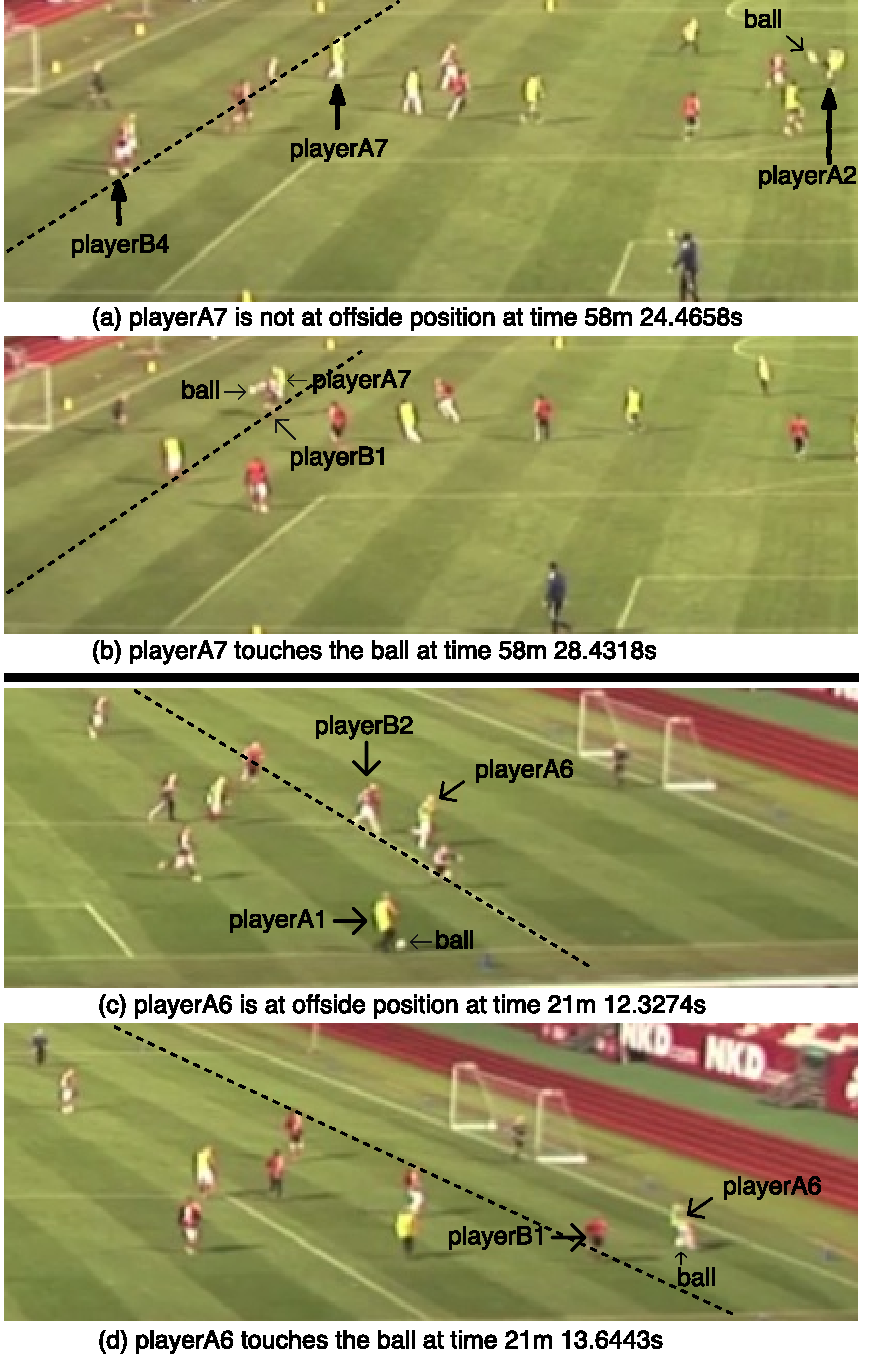
\includegraphics[width=5in]{img/5-fpa}
	\caption{False-positive \& Wrong Foundation Judging Analysis}
	\label{fig:fpa}
\end{figure}

In addition to the results following the process described above, we reviewed the data for the 54:48 case more closely. 
In this case, the nearest player to ball is always Player B4 from 54:44 to 54:46.
However, the distance between Player B4 to ball increases from 59.9 cm to 140 cm, and the video shows that Player B4 touches the ball during that time.
Therefore, we believe that Player B4's sensor failed and lost his position during that time.
This potential sensor failure is not mentioned in DEBS 2013 grand challenge \cite{mutschler2013debs}. 

\begin{table}[!htbp]
\centering
\caption{Strategy Running Performance}
\label{tb:rp}
\begin{tabular}{|l||c|c|c|c|}
\hline
 & *-FI-FO & *-LFU-FO & *-LRU-FO & QR-* \\ \hhline{|=#=|=|=|=|}
Throughput (\#/s) & 497.48 & 306.48 & 328.21 & 381.81 \\ \hline
Eviction Rate (\#/s) & 130.55 & 120.32 & 114.63 & 123.31 \\ \hline
Query Time (s) & 0.34 & 0.30 & 0.33 & 0.18 \\ \hline
Explanation Time (s) & - & 0.03 & 0.03 & 0.03 \\ \hline
QR filtering Time (s) & 0.63 & 0.54 & 0.61 & 0.60 \\ \hhline{|=#=|=|=|=|}
Total Execution Time (s) & 0.97 & 0.87 & 0.97 & 0.81 \\ \hline
\end{tabular}
\end{table}

\begin{table}[!htbp]
\centering
\caption{Strategy Accuracy Analysis}
\label{tb:accuracy}
\begin{tabular}{|c||c|c|c|c|}
\hline
window size $l$ & *-FI-FO & *-LFU-FO & *-LRU-FO & QR-* \\ \hhline{|=#=|=|=|=|}
25\% $l_{max}$ & 0.55 & 0.90 & 0.90 & 0.80 \\ \hline
50\% $l_{max}$ & 0.55 & 0.90 & 0.90 & 0.80 \\ \hline
75\% $l_{max}$ & 0.65 & 0.90 & 0.90 & 0.83 \\ \hline
$l_{max}$ & 0.90 & 0.90 & 0.90 & 0.90 \\ \hline
\end{tabular}
\end{table}

Table \ref{tab:error} summarizes the occurrence ratios of flag errors and non-flag errors when different strategies are in use. 
In the soccer offside terminology, ``flag error'' refers to a wrong offside decision (linesman raises the flag) when there is in fact no offside offence.
Conversely, ``non-flag'' error means that no offside offence is indicated when in fact one occurs. 
The statistical counterparts of the terms ``flag error'' and ``non-flag error'' are our system's false-positive and false-negative judgments, respectively. 
It is worth mentioning that, out of the total 20 cases, there are five judgments given by the referee as ``unsure'' and thus cannot be used as ground-truth. 

\begin{table}[!htbp]
\centering
\caption{Strategy Error Analysis}
\label{tab:error}
\begin{tabular}{|c||c|c|c|c|l|}
\hline
 & *-FI-FO & *-LFU-FO & *-LRU-FO & QR-* & Sys. \\ \hhline{|=#=|=|=|=|=|}
flag err. & 0.07 & 0.00 & 0.00 & 0.02 & 0.02 \\ \hline
non-flag err. & 0.38 & 0.09 & 0.08 & 0.18 & 0.19 \\ \hline
\end{tabular}
\end{table}

Finally, we consider the different scenarios where each type of semantic importance can be applied. 
Generation and expiration timestamps can be applied in a system where recent data is more important, the query is simple, and does not require a history look-up. 
The throughput speed in FIFO benefits the system's real-time response. 
However, if the query is complex and requires history look-ups (as in soccer offside query answering), reasoning participation frequency and recency is better, because they can preserve historical data in the window until other complementary data arrives. 
The trade-off is a relatively lower throughput as a result of the overhead of reasoning and query explanation.
Query relevance filtering has the fastest execution time and also has the most potential to scale.
%
\section{Data Exfiltration Detection}
According to Wikipedia, ``an insider threat is a malicious threat to an organization that comes from people within the organization''\footnote{\url{https://en.wikipedia.org/wiki/Insider\_threat}}. 
Compared to the outside threat, the organization tends to be more vulnerable when facing insider threat. 
This is because the insiders have access to the internal infrastructure, data, or network.
It is very easy for them to steal the organizational intellectual properties.
What makes it even worse is that, the insider threat is much more harder to detect than the outside threat. 
A malicious insider is defined as ``a current or former employee, contractor, or business partner who has or had authorized access to an organization's network, system or data or has intentionally exceeded or intentionally used that access in a manner that negatively affected the confidentiality, integrity, or availability of the organization's information or information systems" \cite{CERT-onto} \cite{silowash2012common}.
This use case aims to detect data exfiltration\footnote{For more details, please refer to the github repository: \url{https://github.com/raymondino/InsiderThreat-StreamReasoningUseCase}.}, a sub-category of insider threat.
%
\subsection{Background}
This use case will focus on one type of insider threat attacks, the data exfiltration. 
According to \cite{CMU-CERT}, the data exfiltration means that a malicious user employs a removable media or the Internet to remove confidential data from an organization.
An example of the data exfiltration is that the employee who finishes work usually around 5:30 PM comes back to the office very late at the night, and uses a removable disk to copy some files or upload the files into wikileaks.org.

There has already been related work that builds methods for data exfiltration. 
\cite{liu2009sidd} proposes a framework called SSID that is based on statistical and signal processing techniques to detect sensitive information distribution and stolen over the Internet. 
\cite{giani2006data} points out that the key for detecting data exfiltration is to identify the distinction between legal and illegal information communication. 
It also provides a detailed list and discussion of most known data exfiltration methods, which is very valuable to model data exfiltration. 
\cite{born2010browser} takes a different way with several novel methods of enabling data exfiltration using web browsers and the JavaScript engine, with the purpose to raise the awareness of this kind of malicious intent. 
%
\subsection{Approach}
Different from the above related work, this use case will be implemented with core notions of stream reasoning, including window and continuous processing, together with the semantic importance model and the sequential stream reasoning architecture. 
A stream reasoning system will be realized to identify and preserve all previous suspicious actions as evidence to determine data exfiltration.
Since the malicious actions can happen across arbitrary interval of time, a logical window will be leveraged. 
This poses a challenge in such a way that the bigger the window size is, the more data will be in the window to negatively affect the system responsiveness. 
In order to enable reasoning, the plan is to leverage and extend the existing insider threat ontology developed by CMU  CERT\footnote{http://www.cert.org/}. 
Semantic importance aspects in provenance and trustworthiness will be selected to support two window management strategies, FIFO and QR-T (query relevance - trustworthiness). 
In order to enable trustworthiness, a simple trust model is established, which will be elaborated in the following section. 
%
\subsection{Data Stream}
Real insider threat datasets are usually very organizational-sensitive and confidential, which makes it not easy to be published. 
However, \cite{glasser2013bridging} provides a synthesized streaming data set that contains four data exfiltration scenarios and provides timestamped employee actions of types including HTTP, device, login, log-off, file and email, which is shown in Figure \ref{fig:dxd}.

\begin{figure}[!htbp]
	\centering
    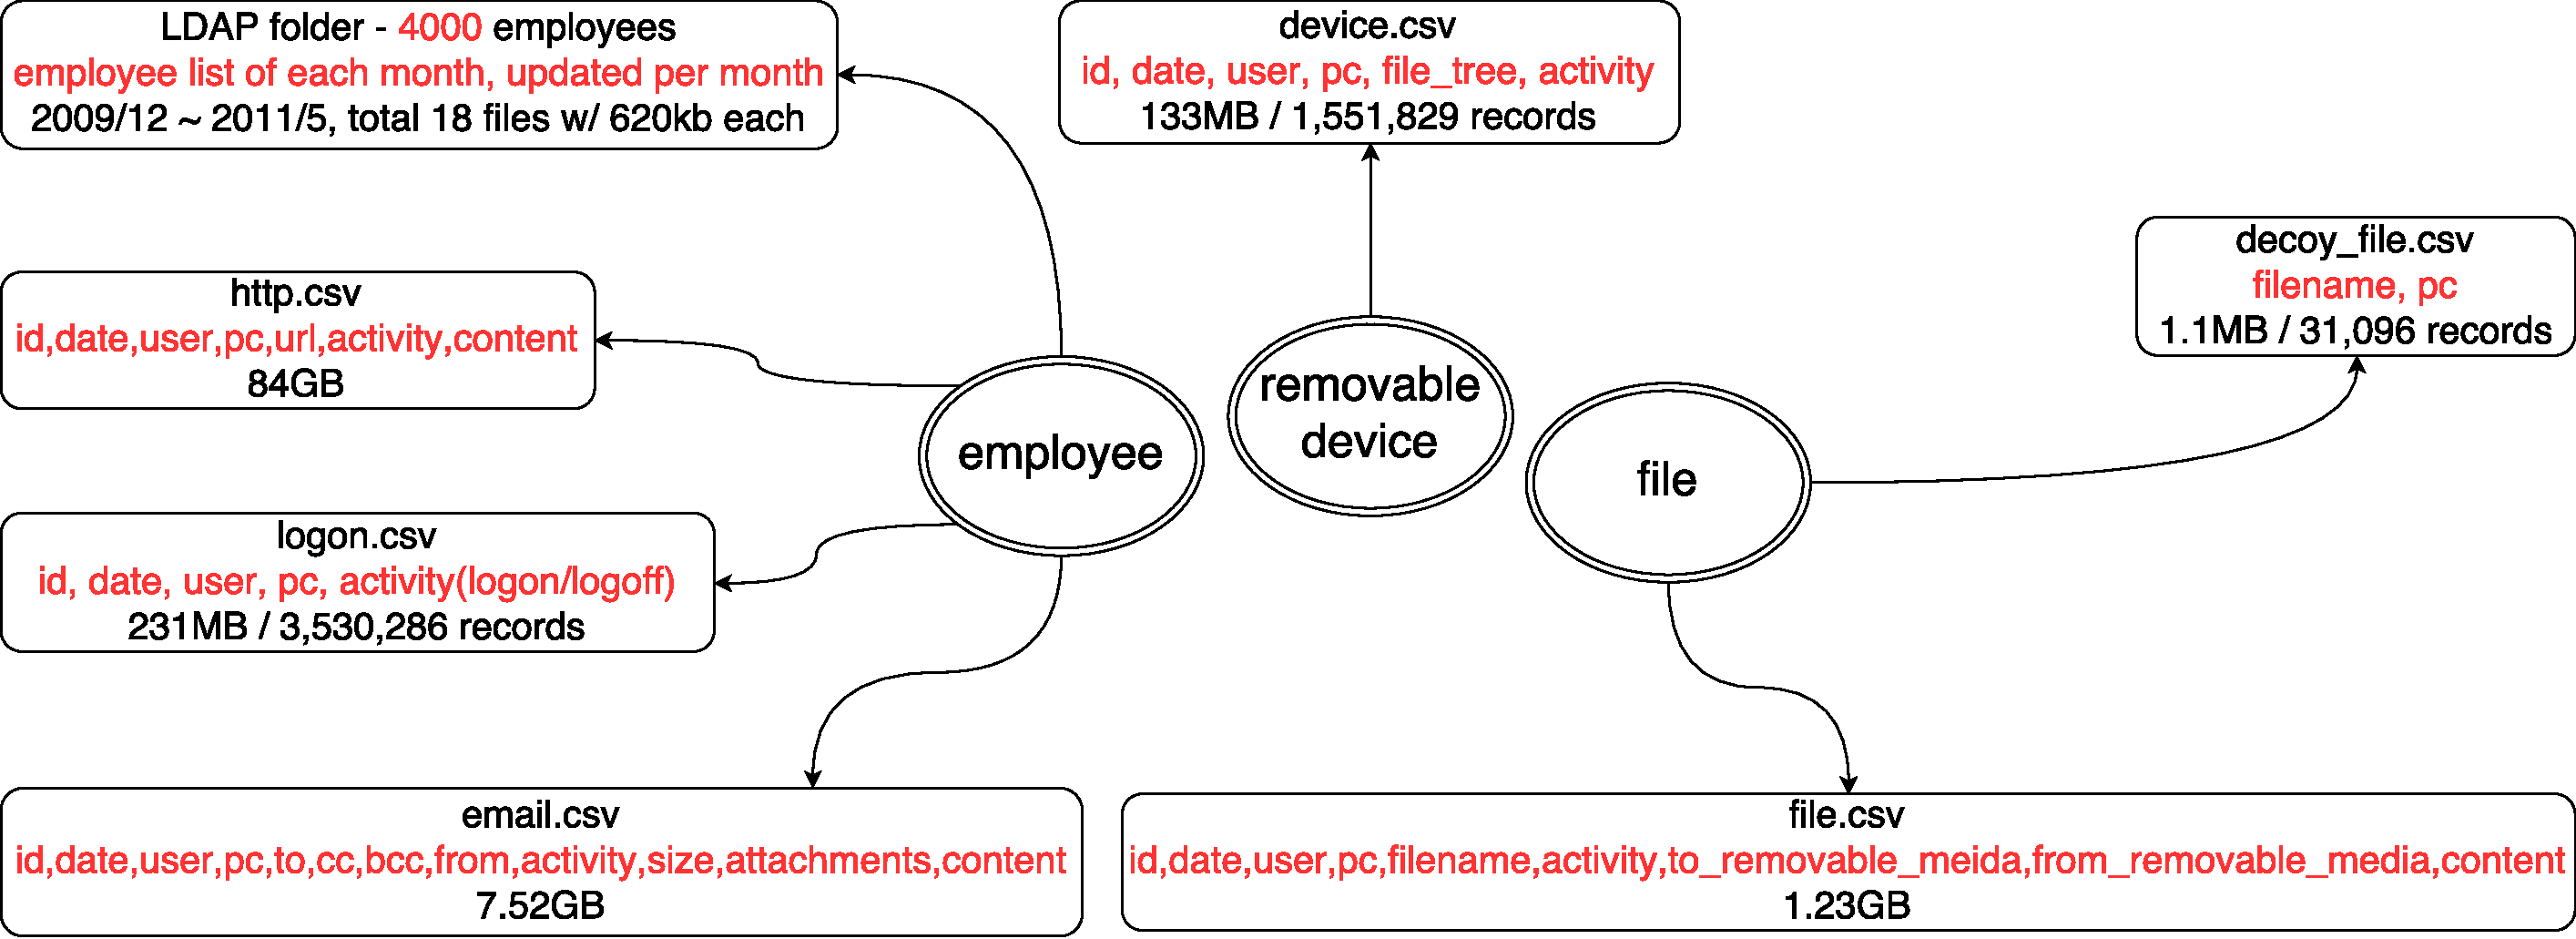
\includegraphics[width=5in]{img/5-dxd.pdf}
    \caption{Synthesized Data for Insider Threat Detection}
    \label{fig:dxd}
\end{figure}

This figure indicates that the dataset is big in size and rich in content. 
It contains 3 categories, the employee data, the removable device data, and the file data. 
An employee can be seen as a sensor that constantly streams action data over a time line, such as HTTP actions including browsing, downloading, and uploading; 
log-on, log-off actions on the organization computers; as well as email actions.
The removable device data includes the actions of using a certain removable device (such as a flash drive) to transfer data.
The file data includes the employee actions performed on the file, such as the contents of the file copied.
There is also some background information provided in the dataset, such as LDAP data in the employee category and the decoy-file data in the file category. 
The LDAP data contains the full list of employees, with their roles, office location and working relationships. 
This list updates weekly. 
The decoy-file data contains the files that are deliberately placed in the employees' working computers, and works like a bait. 
Each dataset has its own data-schema, and is encoded in the comma separated value format.

This dataset provides 4000 users' actions data, in which 5 users are malicious insiders. 
From the given brief scenarios descriptions in the data set, 4 out of 5 malicious insiders are data exfiltration insiders. 
For more details about the dataset, please refer to the \cite{glasser2013bridging} and the website: \url{https://www.cert.org/insider-threat/tools/}.
%
\subsection{Ontology}
CMU CERT has developed an insider threat indicator ontology\footnote{\url{http://resources.sei.cmu.edu/library/asset-view.cfm?assetID=454613}} \cite{costa2014ontology}.
This ontology primarily contains the concepts and relationships that are extracted from their real insider threat use case events database. 
This ontology is leveraged to describe the insider threat scenarios instead of natural language for the purpose of providing structured data for machines to process. 
The ontology doesn't contain any specific concepts to model data exfiltration. 
It is either inconsistent: 
the concept \textbf{TradeSecretInformation} is classified to be both \textbf{Asset} and \textbf{Information}, which are disjoint classes.
In order to extend the CERT ontology, the inconsistency problem needs to be addressed\footnote{I have contacted CMU CERT and provided this feedback to them.}. 
Currently, it is solved by removing the disjointness.
The ontology of this use case is modeled as the figures below. 

\begin{figure}[!htbp]
	\centering
    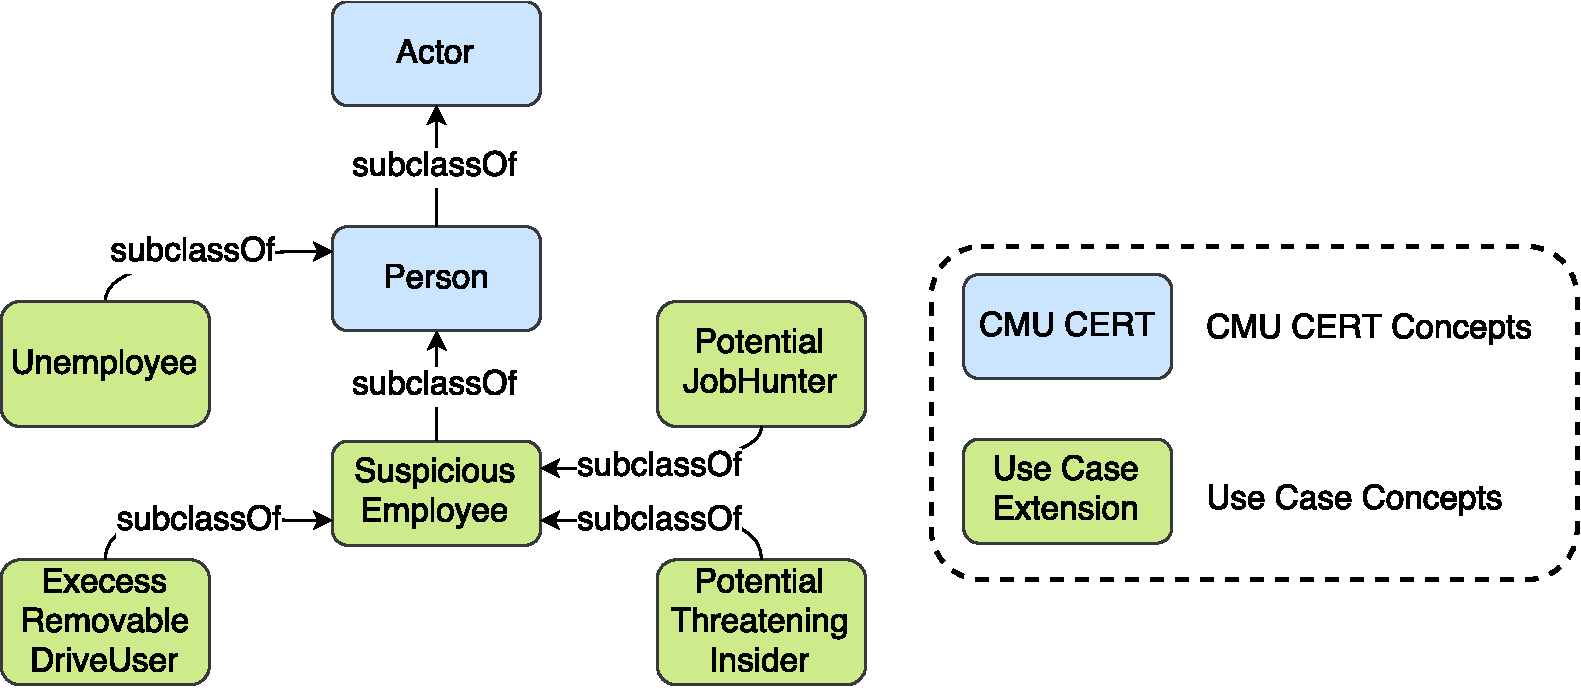
\includegraphics[width=5in]{img/5-dxoactor.pdf}
    \caption{Data Exfiltration Background Ontology: Actor}
    \label{fig:actor}
\end{figure}

Figure \ref{fig:actor} extends the concept \textbf{Actor} by introducing 5 subclasses. 
\textbf{Unemployee} and \textbf{SuspiciousEmployee} are both subclasses of \textbf{Person}.
\textbf{Unemployee} describes previous employees who left the job (either resignation, or laid-off). 
\textbf{SuspiciousEmployee} has three subclasses:
\textbf{ExcessiveRemovableDriveUser} class describes a user who excessively uses the removable disk, compared to his/her normal daily removable disk usage. 
\textbf{PotentialJobHunter} class describes an employee who browsed some job hunting website. 
It's not necessary for an employee to be a jobhunter if he browses job-related website, but the system should be able to record it, then fire an alarm if further suspicious events are detected. 
This class is defined as (\textit{browseWebsite some} \textbf{JobHuntingWebsite}). 
\textbf{PotentialThreateningInsider} class describes a potential threatening insider.
The reason not to name it as something like ``a threatening insider'' is because humans are needed to make the final decision. 
Any users classified into this class will become the forensic target, and is what this use case is looking for. 
This class is defined as (\textit{isInvolvedIn some} \textbf{DataExfiltrationEvent}). 

\begin{figure}[!htbp]
	\centering
    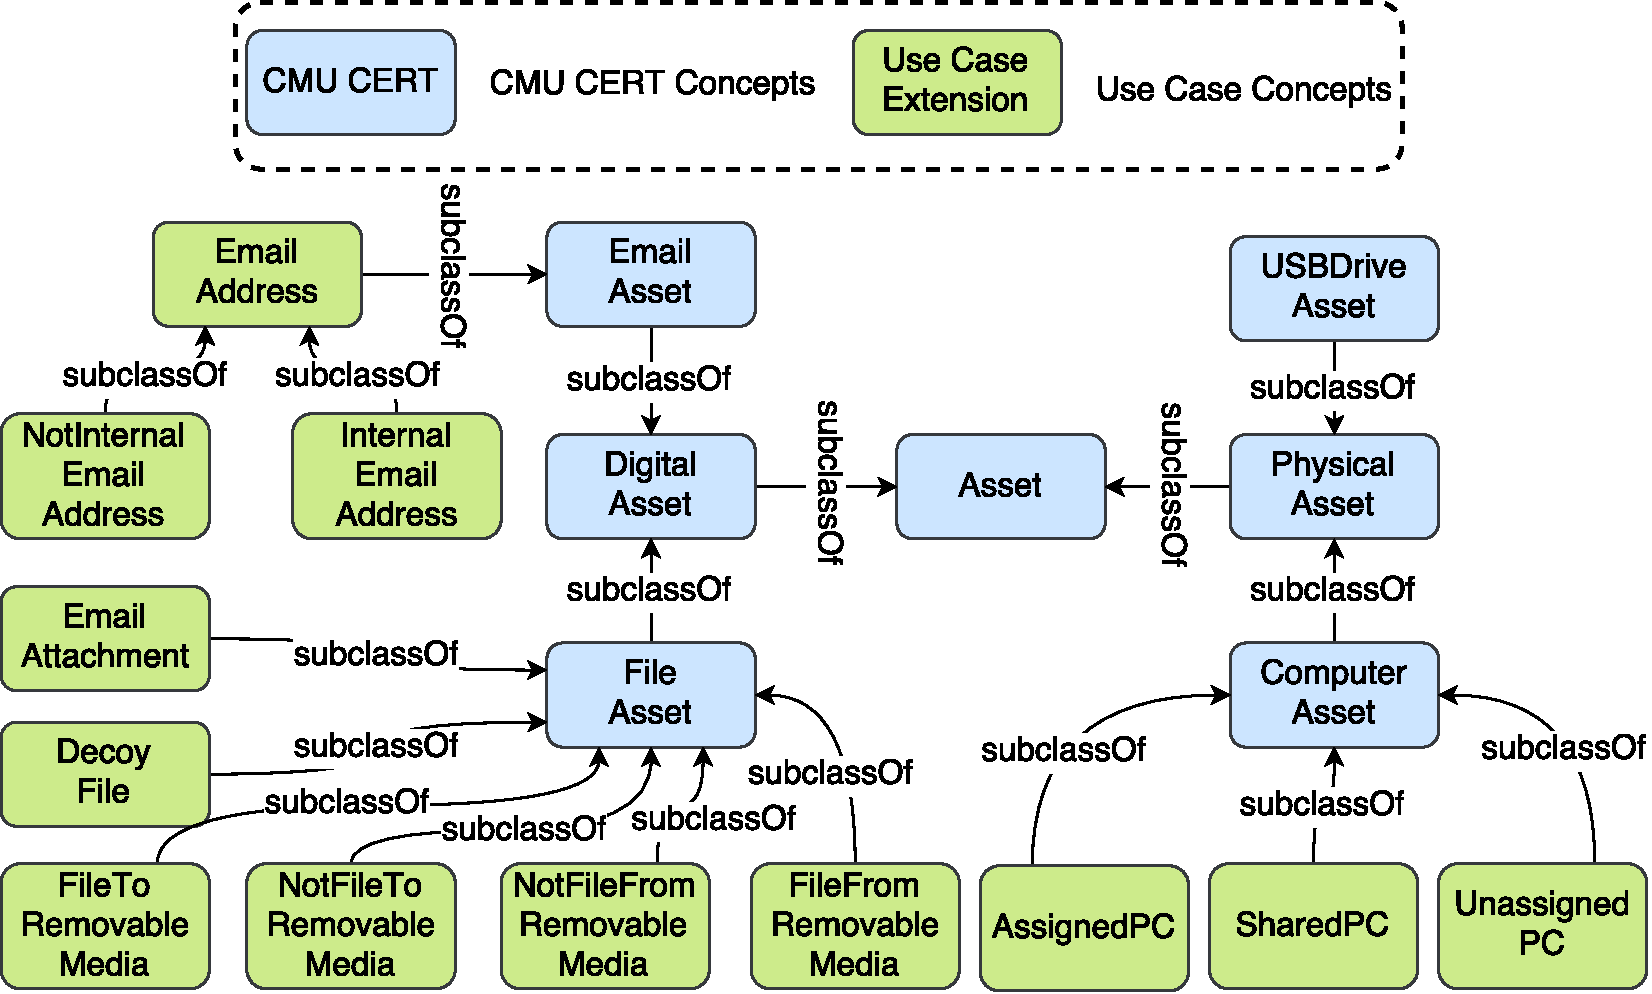
\includegraphics[width=5in]{img/5-dxoasset.pdf}
    \caption{Data Exfiltration Background Ontology: Asset}
    \label{fig:asset}
\end{figure}

Figure \ref{fig:asset} shows the extended models for \textbf{Asset} class.
The focus of using this class is to model the email addresses, files and computers. 
For example, it is important to classify the emails sent to an internal address or an external address. 
It is also crucial to know what kind of file is attached to the email, or copied to/from the flash drive. 
Being able to record which employee uses which computer is also necessary since malicious insiders can possibly get on other employees' computers to steal data. 

\begin{figure}[!htbp]
	\centering
    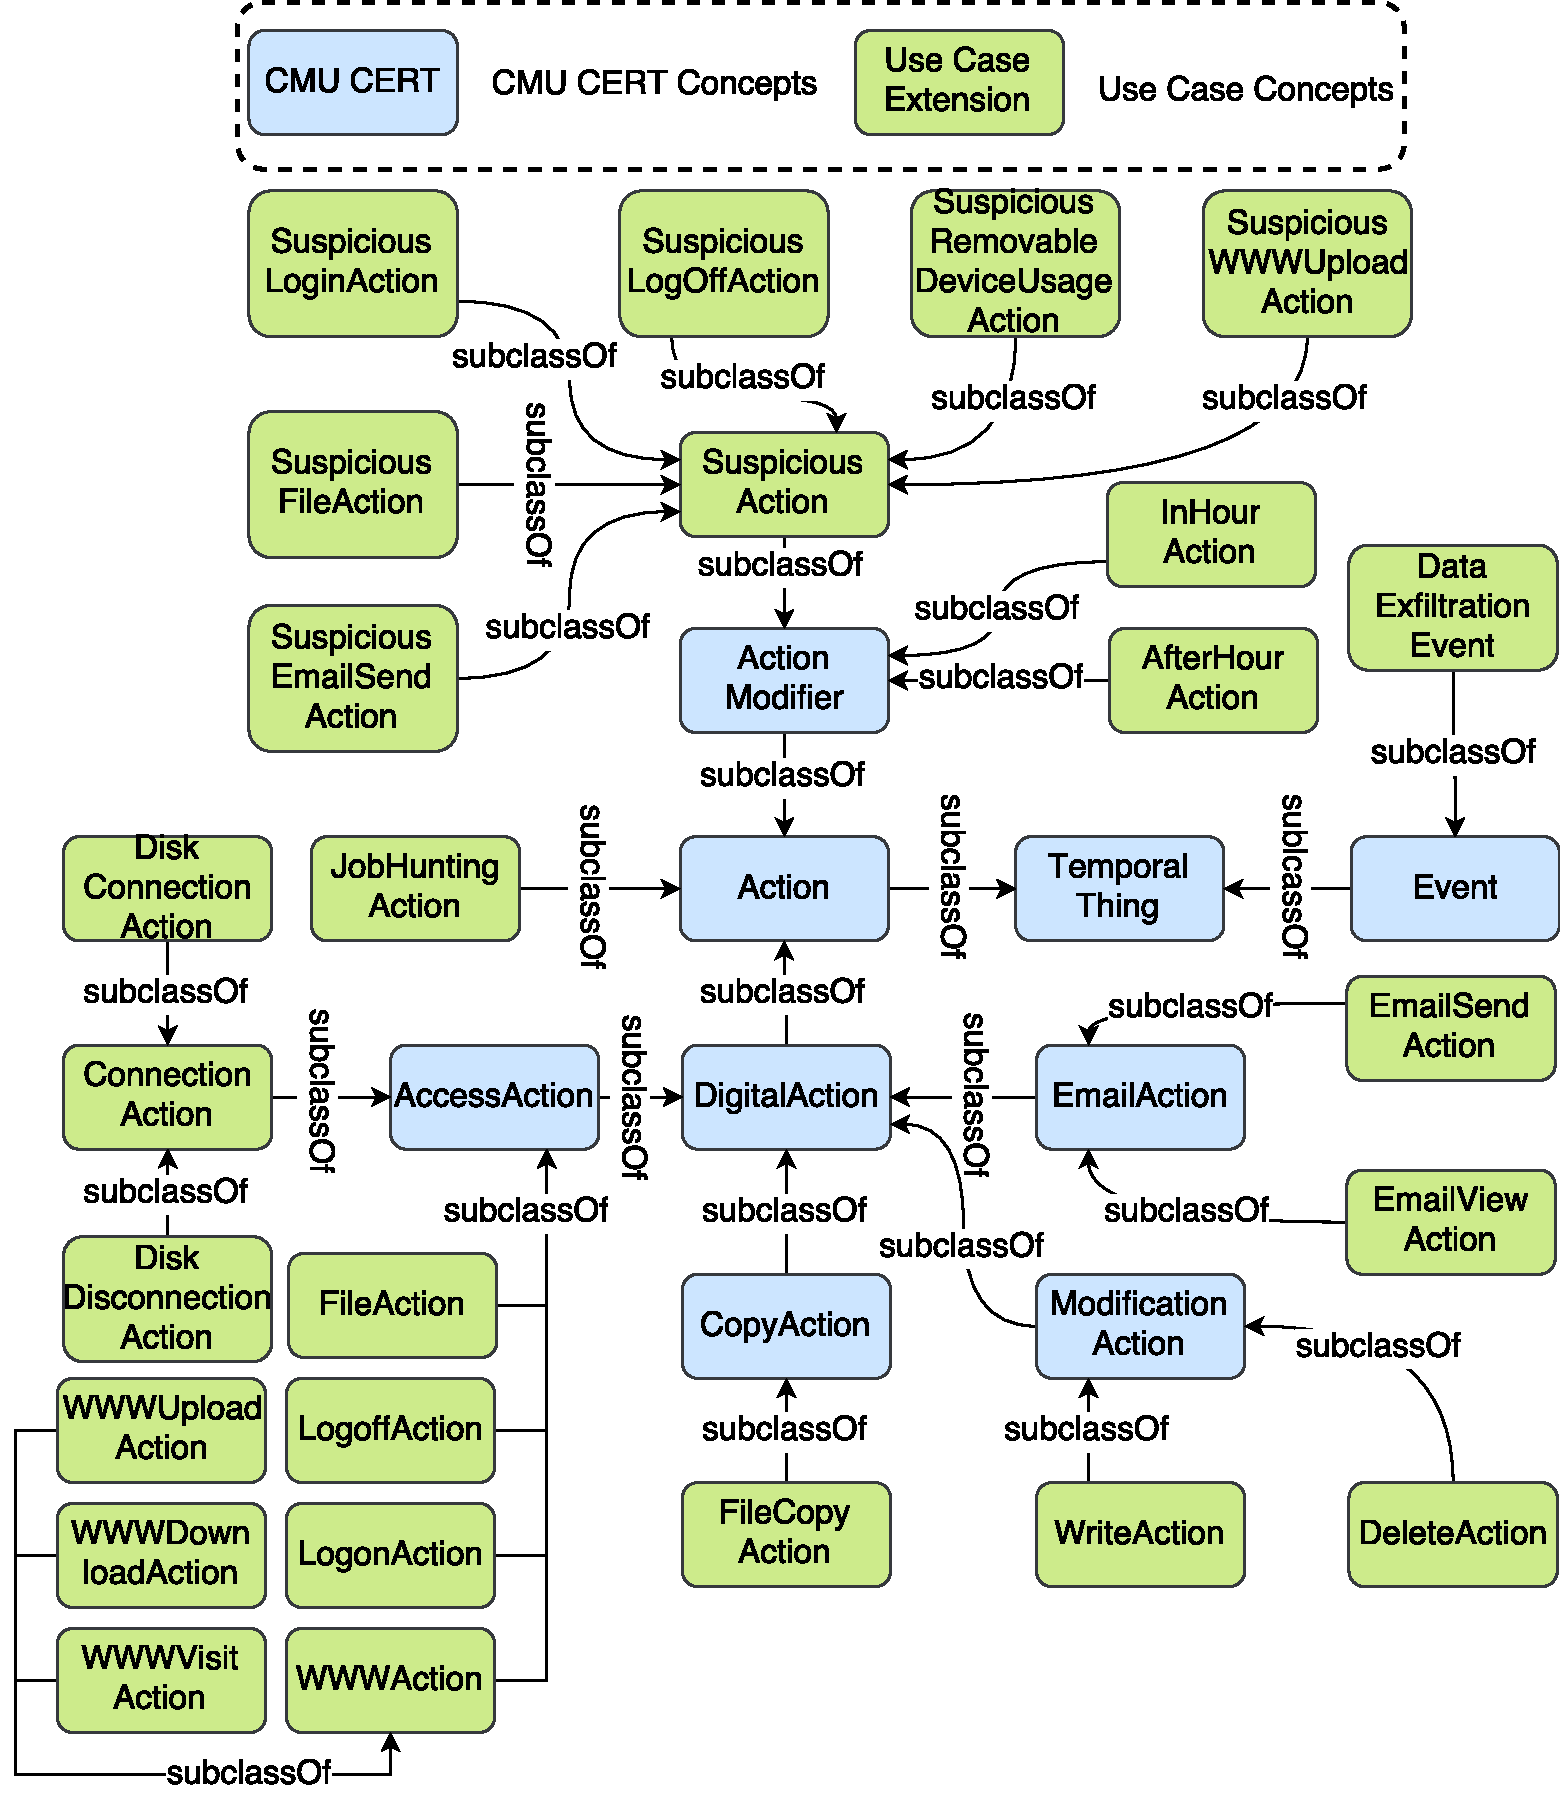
\includegraphics[width=5in]{img/5-dxott.pdf}
    \caption{Data Exfiltration Background Ontology: Temporal Thing}
    \label{fig:tt}
\end{figure}

In the CMU ontology, \textbf{TemporalThing} is the superclass of \textbf{Action} and 
\textbf{Event}, as both of them are time sensitive. 
\textbf{ActionModifier} describes the kinds of the action. 
For example, \textbf{AfterHourAction} describes an action that happens after hour. 
The \textbf{SuspiciousAction} is defined as (\textbf{JobHuntingAction} \textit{or} \textbf{SuspiciousEmailSendAction} \textit{or} \textbf{SuspiciousFileAction} \textit{or} \textbf{SuspiciousLoginAction} \textit{or} \textbf{SuspiciousRemovableDeviceUsageAction} \textit{or} \textbf{SuspiciousWWWUploadAction}). 
This class classifies the defined suspicious actions. 
The reason to include the \textbf{JobHuntingAction} is because a potential job hunter should be taken care of. 
All of the subclasses of \textbf{SuspiciousAction} are defined, which provides the known data exfiltration patterns. 

\textbf{SuspiciousEmailSendAction} is defined as (\textbf{EmailSendAction} \textit{and} ((\textit{bcc some} \textbf{NotInternalEmailAddress}) \textit{or} (\textit{cc some} \textbf{NotInternalEmailAddress}) \textit{or} (\textit{from some} \textbf{NotInternalEmailAddress}) \textit{or} (\textit{to some} \textbf{NotInternalEmailAddress}))) \textit{or} (\textit{hasEmailAttachment some} \textbf{DecoyFile}).
It takes care of those emails sent to external email addresses. 

\textbf{SuspiciousFileAction} is defined as (\textbf{AfterHourAction} \textit{and} ( \textbf{FileCopyAction} \textit{or} \textbf{FileDeleteAction} \textit{or} \textbf{FileOpenAction})) \textit{or} (\textbf{FileCopyAction} \textit{and} (\textit{hasFile some} \textbf{DecoyFile})) \textit{or} (((\textit{isPerformedOnPC some} \textbf{UnassignedPC}) \textit{and} \textbf{FileCopyAction} \textit{or} \textbf{FileDeleteAction} \textit{or}  \textbf{FileOpenAction})) \textit{or} (\textit{startsNoEarlierThanEndingOf some} \textbf{SuspiciousRemovableDeviceUsageAction}). 
Basically, a suspicious file action is an action that either is performed after hour by deleting, copying or opening a decoy file, or using a removable drive to delete, copy, or open files on an unassigned PC. 

\textbf{SuspiciousLoginAction} is defined as (\textbf{AfterHourAction} \textit{and} \textbf{LogonAction}) \textit{or} (\textbf{LogonAction} \textit{and} (\textit{isPerformedOnPC some} \textbf{UnassignedPC})).
This means that any action that is performed after hours or on an unassigned PC will be classified as a suspicious login action. 
Similarly, \textbf{SuspiciousLogoffAction} is defined as (\textbf{AfterHourAction} \textit{and} \textbf{LogoffAction}) \textit{or} (\textbf{LogoffAction} \textit{and} (\textit{isPerformedOnPC some} \textbf{UnassignedPC})).

\textbf{SuspiciousRemovableDeviceUsageAction} is defined as ( \textbf{AfterHourAction} \textit{and} (\textbf{DiskConnectionAction} \textit{or} \textbf{DiskDisconnectionAction})) \textit{or} ((\textbf{DiskC\\onnectionAction} \textit{or} \textbf{DiskDisconnectionAction}) \textit{and} (\textit{isPerformedOnUnassign\\edPC some} \textbf{UnassignedPC})) \textit{or} (\textit{hasActor some} \textbf{ExcessiveRemovableDriveUs\\er}).
This class will classify the actions that are performed either after hours with a disk connection action, or from an excessive removable driver user. 

\textbf{SuspiciousWWWUploadAction} is defined as (\textbf{AfterHourAction} \textit{and} \textbf{W\\WWUploadAction}) \textit{or} (\textbf{WWWUploadAction} \textit{and} (\textit{hasWebsite some} (\textbf{Cloud\\StorageWebsite} \textit{or} \textbf{HacktivistWebsite}))) \textit{or} ((\textbf{WWWDownloadAction} \textit{or} \textbf{WWWUploadAction} \textit{or} \textbf{WWWVisitAction}) \textit{and} (\textit{isPerformedOnUnassigned\\PC some} \textbf{Unassigned-PC})).
It describes a kind of malicious action that a user uploads files to cloud storage or hactivist website after-hour or from an unsigned PC.

\textbf{DataExfiltrationEvent} class is the subclass of \textbf{Event}. 
It describes the data exfiltration event, and is defined as ((((\textit{hasAction min 10} \textbf{SuspiciousEmailSendAction}) \textit{and} (\textit{hasAction max 10000} \textbf{SuspiciousEmailSendAction})) \textit{or} (\textit{hasAction max 10000} \textbf{SuspiciousWWWUploadAction})) \textit{and} (\textit{hasAction min 5} \textbf{SuspiciousWWWUploadAction})) \textit{or} ((\textit{hasAction min 3} \textbf{SuspiciousFileAction}) \textit{and} (\textit{hasAction max 10000} \textbf{SuspiciousFileAction})).
In its definition, cardinality is used to quantify a threshold to determine a data exfiltration event.

Last but not the least, the ontology has a \textbf{Website} class that models different websites. 
It has four subclasses, \textbf{CloudStorageWebsite} that describes sites like dropbox.com; 
\textbf{HacktivistWebsite} that describes sites like wikileaks.org;
\textbf{JobHuntingWebsite} that describes sites like indeed.com;
and \textbf{NeutralWebsite} that describes sites other than the above three. 

\subsection{Data Annotation}
Data is pre-processed before annotated by the data exfiltration background ontology. 
All employees' routine hours are calculated based on their first two week working hours. 
This routine hours will be used as a basis of judging the after hour actions. 
Also, employees' routine log-on/log-off time, and daily removable disk usage situations are extracted for reference. 
In the LDAP folder of the synthesized dataset, a employee list is provided for every month.
This list is updated monthly, thus employees who are not in current month LDAP list will be annotated as an instance of \textbf{Unemployee}.

Logon.csv file follows the schema of (id, date, user, pc, activity), where ``id'' is the unique action id, ``date'' is a xsd:dateTime timestamp indicating the generation timestamp of the action, ``user'' is the employee id, ``pc'' is where the action is performed, ``activity'' is a string of either logon or logoff. 
Thus, the data in Logon.csv file can be annotated in RDF stream as follows: \\
(1) :$<$user$>$-event :hasAction :$<$activity$>$\_$<$id$>$, $<$date$>$. \\
(2) :$<$activity$>$\_$<$id$>$ rdf:type :Action, $<$date$>$. \\
(3) if $<$date$>$ is not in normal working hours of $<$user$>$, \\
:$<$activity$>$\_$<$id$>$ rdf:type :AfterHourAction, $<$date$>$; \\ 
else, :$<$activity$>$\_$<$id$>$ rdf:type :InHourAction, $<$date$>$. \\
(4) :$<$activity$>$\_$<$id$>$ :hasActor :$<$user$>$, $<$date$>$.  \\
(5) :$<$activity$>$\_$<$id$>$ :isPerformedOnPC :$<$pc$>$, $<$date$>$. 

Device.csv file has the schema of (id, date, user, pc, file\_tree, activity), where ``id, date, user, pc'' are the same as Logon.csv.
``file\_tree'' is the directory content of the removable drive.
``activity'' describes the action taken by the user. 
The data is annotated as follows: \\
(1) :$<$user$>$-event :hasAction :device\_$<$activity$>$\_$<$id$>$, $<$date$>$. \\
(2) if current employee's daily removable device usage count is bigger than his/her routine usage, then annotate \\
:$<$user$>$ rdf:type :ExcessiveRemovableDriveUser, $<$date$>$. \\
(3) :device\_$<$activity$>$\_$<$id$>$ rdf:type :Action, $<$date$>$. \\
(4) if $<$date$>$ is not in the normal working hours of $<$user$>$, \\
:device\_$<$activity$>$\_$<$id$>$ rdf:type :AfterHourAction, $<$date$>$; \\
else, :device\_$<$activity$>$\_$<$id$>$ rdf:type :InHourAction, $<$date$>$. \\
(5) :device\_$<$activity$>$\_$<$id$>$ :hasActor :$<$user$>$, $<$date$>$. \\
(6) :device\_$<$activity$>$\_$<$id$>$ :isPerformedOnPC :$<$pc$>$, $<$date$>$. \\
(7) if the activity is ``connect'', \\
:device\_$<$activity$>$\_$<$id$>$ :isPerformedWithRemovableDisk \\
:device\_$<$activity$>$\_$<$id$>$\_disk, $<$date$>$. 

Email.csv file encodes data with the schema of (id, date, user, pc, to, cc, bcc, from, activity, size, attachments, content), where ``id, date, user, pc'' are the same as above. 
``to, cc, bcc, from'' respectively indicates the sender's and receivers' email addresses, ``activity'' is either send or view, ``size'' is the attachment's size in bytes, ``attachments'' refer to the attached files in the email, ``content'' indicates the contents in the email. 
The data is annotated as follows: \\
(1) $<$user$>$-event :hasAction :email\_$<$activity$>$\_$<$id$>$, $<$date$>$. \\
(2) :email\_$<$activity$>$\_$<$id$>$ rdf:type :EmailAction, $<$date$>$. \\
(3) if $<$date$>$ is not in the normal working hours, \\
:email\_$<$activity$>$\_$<$id$>$ rdf:type :AfterHourAction, $<$date$>$; \\
else, :email\_$<$activity$>$\_$<$id$>$ rdf:type :InHourAction, $<$date$>$. \\ 
(4) :email\_$<$activity$>$\_$<$id$>$ :hasActor $<$user$>$, $<$date$>$. \\
(5) :email\_$<$activity$>$\_$<$id$>$ :isPerformedOnPC $<$pc$>$, $<$date$>$.\\ 
(6) :email\_$<$activity$>$\_$<$id$>$ :to :$<$to$>$, $<$date$>$,\\
(7) :email\_$<$activity$>$\_$<$id$>$ :cc :$<$cc$>$, $<$date$>$. \\
(8) :email\_$<$activity$>$\_$<$id$>$ :bcc :$<$bcc$>$, $<$date$<$. \\
(9) :email\_$<$activity$>$\_$<$id$>$ :from :$<$from$>$, $<$date$>$. \\
(10) if the email address ($<$email-address$>$ includes $<$to$>$, $<$cc$>$, $<$bcc$>$, and $<$from$>$) is the organization address,\\
:$<$email-address$>$ rdf:type :InternalEmailAddress;\\
else, :$<$email-address$>$ rdf:type :ExternalEmailAddress.\\ 
(11) :email\_$<$activity$>$\_$<$id$>$ :hasEmailAttachment :$<$attachments$>$, $<$date$>$. \\
(12) :$<$attachments$>$ :hasSize :$<$size$>$, $<$date$>$.\\
(13) :email\_$<$activity$>$\_$<$id$>$ :hasContent :$<$content$>$, $<$date$>$. 

File.csv file contains the data schema of (id, date, user, pc, filename, activity, to\_removable\_media, from\_removable\_media, content), where ``id, date, user, pc'' are the same as the above.
``filename'' describes the name of the file, ``activity'' denotes the action performed on the file, ``to\_removable\_media'' denotes if the file is performed to the removable media, ``from\_removable\_media'' is the opposite, ``content'' describes the file content. 
The data is annotated as follows: \\
(1) :$<$user$>$-event :hasAction :file\_$<$activity$>$\_$<$id$>$, $<$date$>$. \\
(2) :file\_$<$activity$>$\_$<$id$>$ rdf:type :FileAction, $<$date$>$. \\
(3) if $<$date$>$ is not within the normal working hours, \\
:file\_$<$activity$>$\_$<$id$>$ rdf:type :AfterHourAction, $<$date$>$;\\
else, :file\_$<$activity$>$\_$<$id$>$ rdf:type :InHourAction, $<$date$>$.\\ 
(4) :file\_$<$activity$>$\_$<$id$>$ :hasActor :$<$user$>$, $<$date$>$. \\
(5) :file\_$<$activity$>$\_$<$id$>$ :isPerformedOnPC :$<$pc$>$, $<$date$>$. \\
(6) :file\_$<$activity$>$\_$<$id$>$ :hasFile :$<$filename$>$, $<$date$>$.\\
(7) if ``to\_removable\_media" is true, \\
:$<$filename$>$ rdf:type :FileToRemovableMedia, $<$date$>$;\\
else, $<$filename$>$ rdf:type NotFileToRemovableMedia, $<$date$>$.\\ 
(8) if ``from\_removable\_media'' is true,\\
:$<$filename$>$ rdf:type :FileFromRemovableMedia, $<$date$>$;\\
else, $<$filename$>$ rdf:type :NotFileFromRemovableMedia, $<$date$>$. 

Decoy.csv has the data schema of ``filename, pc'', where ``filename'' is the name of the decoy file, ``pc'' is where the file is located.
Decoy.csv file is used as the background information, thus no timestamps are associated. 
Data is annotated as: \\
(1) :$<$filename$>$ rdf:type :DecoyFile. \\
(2) :$<$filename$>$ :isIn $<$pc$>$. 

LDAP folder contains 18 files, each of which is a list of employees during that month.
They record from 2009/12 to 2011/05.
The employee list is updated monthly.
These files are used as the background information. 
Each file is with a data schema of (employee\_name, user\_id, email, role, projects, business\_unit, functional\_unit, department, team, supervisor).
Thus the data is annotated as: \\
(1) :$<$user\_id$>$ :hasName :$<$employee\_name$>$. \\
(2) :$<$user\_id$>$ :hasEmailAddress :$<$email$>$. \\
(3) :$<$user\_id$>$ :hasRole :$<$role$>$. \\
(4) :$<$user\_id$>$ :hasProjects :$<$projects$>$. \\
(5) :$<$user\_id$>$ :hasBusinessUnit :$<$business\_unit$>$. \\
(6) :$<$user\_id$>$ :hasFunctionalUnit :$<$functional\_unit$>$. \\
(7) :$<$user\_id$>$ :hasDepartment :$<$department$>$. \\
(8) :$<$user\_id$>$ :hasTeam :$<$team$>$. \\
(9) :$<$user\_id$>$ :hasSupervisor :$<$supervisor$>$.

Http.csv file has the schema of ``id, date, user, pc, url, activity, content'', where ``id, date, user, pc'' are the same as the above. 
``url'' is the link that the user visits, ``activity'' is either view, upload, and download, ``content'' is the content of the web-page browsed. 
The data is annotated as follows:\\
(1) :$<$user$>$-event :hasAction :http\_$<$activity$>$\_$<$id$>$, $<$date$>$.\\
(2) :http\_$<$activity$>$\_$<$id$>$ rdf:type :Action, $<$date$>$.\\
(3) if $<$date$>$ is within the routine hours of the user, \\
:http\_$<$activity$>$\_$<$id$>$ rdf:type :InHourAction, $<$date$>$;\\
else, :http\_$<$activity$>$\_$<$id$>$ rdf:type :AfterHourAction, $<$date$>$.\\
(4) :http\_$<$activity$>$\_$<$id$>$ :hasActor :$<$user$>$, $<$date$>$.\\
(5) :http\_$<$activity$>$\_$<$id$>$ :isPerformedOnPC :$<$pc$>$, $<$date$>$.\\
(6) :http\_$<$activity$>$\_$<$id$>$ :hasURL :$<$url$>$, $<$date$>$.\\
(7) URLs are annotated with \textbf{Website} class: \\
:$<$url$>$ :whoseDomainNameIsA :cloudstoragewebsite \\
:$<$url$>$ :whoseDomainNameIsA :hacktivistwebsite \\
:$<$url$>$ :whoseDomainNameIsA :jobhuntingwebsite \\
:$<$url$>$ :whoseDomainNameIsA :neutralwebsite.
%
\subsection{System Implementation}
The data exfiltration detection system is implemented on the basis of the sequential stream reasoning architecture. 
A lower-bounded landmark logical window is deployed in the system. 
The advantage of the landmark window is reflected incisively and vividly in this use case. 
For data exfiltration detection, the malicious insiders can do harm to the organization in any arbitrary time period, which makes determining the size for the conventional logical sliding window very challenging: a small size probably will not provide good precision, but a big size will result in more data that hinders the system performance. 
A landmark window, on the other hand, can retain the useful data when evicting other data, and can work with various window management strategies. 

The query is to look for suspicious actions, which is shown in Listing 5.5. 
This query involves the background data such as LDAP, the streaming data annotated by the background ontology as well as the background ontology itself.
This query requires DL reasoning. 

\begin{lstlisting}[language=SPARQL,caption={Suspicious Action Query},basicstyle=\small, frame=single]
PREFIX de:<http://tw.rpi.edu/ontology/DataExfiltration/>
SELECT DISTINCT ?action 
WHERE { ?action a de:SuspiciousAction.}
\end{lstlisting}

Employees who performed the detected suspicious actions will be recorded, together with the actions he/she performs. 
All of the records will be printed to the screen, written to the event log, and make it easier for humans to make a final judgment. 
However, detecting suspicious actions is not the ultimate goal of this use case.
In the background ontology, the data exfiltration event is defined with cardinalities.
If an employee performs suspicious actions several times, then this employee is a potential malicious insider, and should be paid special attention to. 
Thus, another query in Listing 5.6 examines the employees' performed suspicious actions and checks if he/she is a potential malicious insider. 
This query is parameterized, where $<$user$>$ will be filled during the run time. 
If this query returns true, then the user will be reported. 
The query also requires DL reasoning. 

\begin{lstlisting}[language=SPARQL, caption={Potential Malicious Insider Query},basicstyle=\small,frame=single]
PREFIX de:<http://tw.rpi.edu/ontology/DataExfiltration/>
ASK WHERE { de:<user> a de:PotentialThreateningInsider.}
\end{lstlisting}

This use case has chosen provenance and trustworthiness from semantic importance to form two window management strategies, FIFO and QR-T. 
FIFO is first in first out, its priority vector is [$\tau_{a}$]; 
while QR-T is query relevance trustworthiness, its priority vector is [$qrf, t^{tm}_{s}$]
The reason to choose query relevance is because of the large amount of the streaming data. 
There is really a need to identify, and filter out the unnecessary data to improve system response. 
Thus, a query relevance ontology is provided. 
In the previous section, it is mentioned that this query relevance ontology is query-informed.
However, for this use case, no dedicated query relevance ontology is provided, as the background domain ontology has already provided enough information to filter out the data. 
In this use case, the background domain ontology can be used as a query relevance ontology. 
For example, the query in Listing 5.5 really looks for the suspicious actions. 
As the action data keeps streaming into the system, each action data item will be examined by the query engine, and if that action data item is not classified as a suspicious action, it can be immediately dropped without having to enter into the window.
Only those suspicious action instances will be entered into the window. 
One important thing to note is that, the reason this use case implementation can realize query relevance filtering with a background ontology is very use case specific, and should not be seen as a general solution. 
This use case can do this because the background ontology has already provide enough information, as well as the system working mechanism that each action data item will be examined before entering into the window. 

A simple trust mode has been developed because the existing models are very heterogeneous, and not usually applicable for the scenario of this use case. 
The trust model works in this way: 
initially, each employee has a trust score of $t_{s_i}$. 
As the system runs, if an employee A performed a suspicious action, his/her trust score will reduce 1. 
There is a threshold Y, such that $0 < Y < t_{s_i}$. 
If A's $t^{A}_{s_i}$ is smaller than Y, then  employee A becomes untrusted, thus all of his/her actions will be recorded and sent to the administrators to analyze. 
The QR-T strategy firstly filters out the unnecessary action data, then ranks the action data according to their actors' trust scores. 
%
\subsection{Evaluation}
The window has been set to detect the period of 1 day, 1 week and 1 month for any suspicious actions and malicious users. 
Two strategies are deployed, and evaluated via recording the precision, recall, and the running time. 

\begin{table}[!htbp]
	\centering
    \caption{Strategy Performance}
    \label{tab:sp}
    \begin{tabular}{|c||c|c|} \hline
    	& precision & recall \\ \hhline{|=#=|=|}
        FIFO (1D) & 0.18 & 0.93 \\ \hline
        QR-T (1D) & 0.18 & 0.97 \\ \hline
        FIFO (1W) & 0.26 & 0.87 \\ \hline
        QR-T (1W) & 0.26 & 0.95 \\ \hline
        FIFO (1M) & 0.26 & 0.87 \\ \hline
        QR-T (1M) & 0.26 & 0.95 \\ \hline
    \end{tabular}
\end{table}

Table \ref{tab:sp} shows the system precision and recall. 
The precision of FIFO and QR-T are equal for the same detection time period, and slightly increases as the time-period becomes bigger. 
QR-T's recall is always better than that of FIFO for the same detection time period. 
The precision, undoubtedly, is very low. 
There are reasons for that. 
Insider threat is by no means a simple problem that can be solved with only stream reasoning technologies, it should at least include natural language processing, machine learning and possibily some other technologies. 
The known pattern on data exfiltration is not very discriminative.
That a person who uses a removable disk to copy some file and then upload it into dropbox could be either malicious or innocent.
Thus the background ontology cannot do a good job in classifying data exfiltration actions.

\begin{table}[!htbp]
	\centering
    \caption{Strategy Running Time}
    \label{tab:srt}
    \begin{tabular}{|c||c|c|} \hline
	    & FIFO & QR-T \\ \hhline{|=#=|=|}
    	$T_{total}$ & 49.94 (ms) & 29.63 (ms) \\ \hline    
    \end{tabular}	
\end{table}

However, this use case implementation shows a positive example in Table \ref{tab:srt}, where clearly QR-T runs faster than FIFO. 
This is because FIFO strategy has more data in the window than QR-T, which slows down the running performance.
The results have shown that semantic importance enabled window management strategy can improve the system response time. 
%
\section{Discussion}
This section covers the two use case implementations using both semantic importance and sequential stream reasoning architecture.
From the result tables, a significant difference can be seen in the system outputs from different window management strategies enabled by different semantic importance aspects. 
The two use cases, albeit are from two different domains, share similar characters. 
The streaming data is big for both cases. 
The offside use case data updates frequently, while the data exfiltration data is massive due to frequent actions from many employees. 
Also, it requires complex DL reasoning in both cases. 
Streaming data alone, although provides the basic semantics from the ontology annotation, is not able to provide the desired results. 
From the results, we can see that semantic importance is able to improve the system precision, memory consumption, and response time.

However, one should also see that the implementations of both use cases are dependent upon very specific assumptions that are only applicable in specific scenarios.
This limits the generalization of semantic importance. 
The topics of generalizing and benchmarking semantic importance will be covered in the next chapter. 
%%%%%%%%%%%%%%%%%%%%%%%%%%%%%%%%%%%%%%%%%%%%%%%%%%%%%%%%%%%%%%%%%%%% 
%                                                                 %
%                            CHAPTER SIX                          %
%                                                                 %
%%%%%%%%%%%%%%%%%%%%%%%%%%%%%%%%%%%%%%%%%%%%%%%%%%%%%%%%%%%%%%%%%%% 
\chapter{SEMANTIC IMPORTANCE GENERALIZATION AND BENCHMARK}
The sequential stream reasoning architecture (SSRA) is an innovative architecture that is designed and implemented specifically for stream reasoning use cases aiming to mine the knowledge in the boundless and torrent streaming data. 
Based on SSRA, two use cases are implemented, which to some extent demonstrates the usefulness of the semantic importance in the stream reasoning context. 
However, SSRA implementations are only evaluated out of commercial triple-store products, also only three strategies and a few of semantic importance aspects are tested.
In addition, specific case-by-case assumptions are applied in the use case implementations.
The experimental results have shown some evidence to support the advancement of the semantic importance.

The silent assumption, as well as the early eviction and expiration problems altogether demonstrate why people should care about semantic importance. 
This chapter focuses on quantifying the benefits, pointing out the  limitations of semantic importance, and demonstrating what it takes to reuse and extend semantic importance.
The core contribution in this chapter is a generalization and benchmark framework called \textbf{SIGenBench}. 
It generalizes semantic importance by connecting it to the state-of-the-art stream reasoning techniques.
It also features a flexible benchmark system that can be configured to adapt with different stream reasoning scenarios. 
This benchmark reports four system key performance metrics including memory consumption, response time, precision, and throughput, with which the impacts and benefits of semantic importance are discussed in details.  
%
\section{Introduction}
Figure \ref{fig:6-sib} shows the architecture of SIGenBench.
SIGenBench is implemented based on SSRA, and provides two main functionalities: generalization (blue) and benchmark (green).
Generalization refers to reusability, i.e. how semantic importance can be reused in different use cases.
Benchmark refers to usefulness, i.e. how semantic importance can be useful in various stream reasoning settings.

\begin{figure}[!htbp]
	\centering
    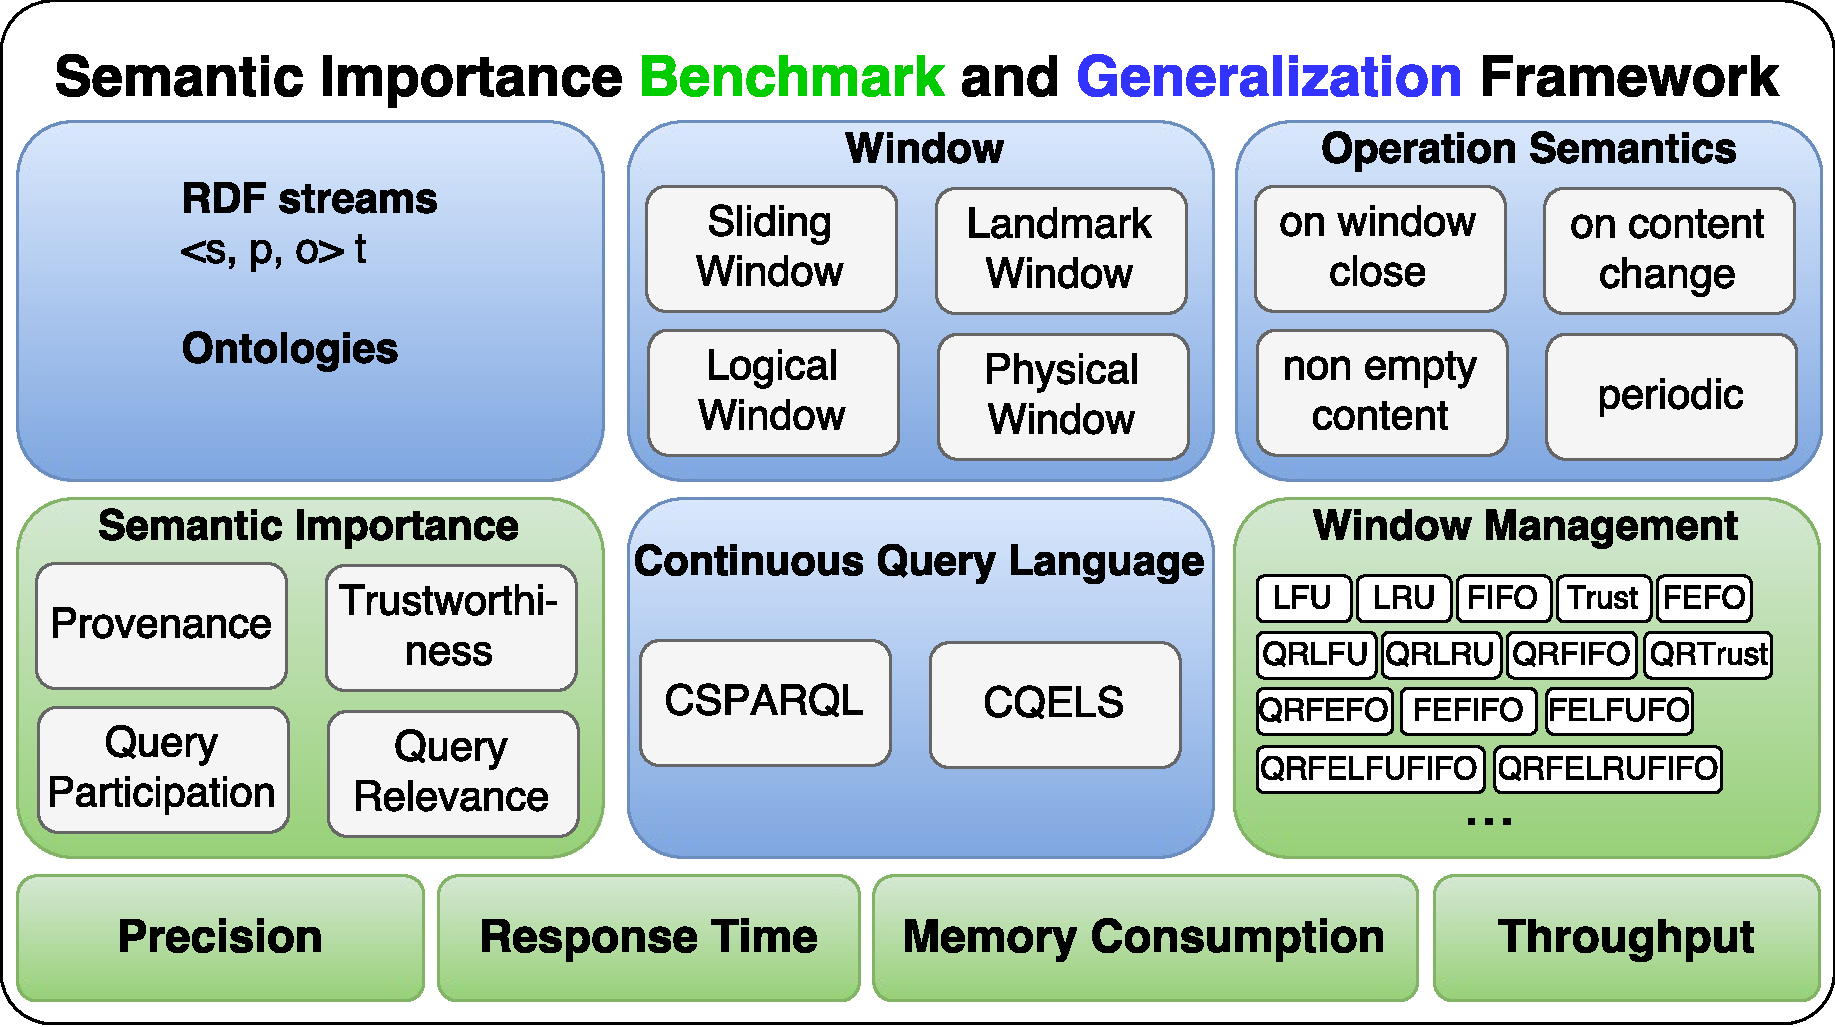
\includegraphics[width=5in]{img/6-sib.pdf}
    \caption{\textbf{SIGenBench Architecture}}
    \label{fig:6-sib}
\end{figure}

In order to enable generalization, semantic importance ontology (SIO) is created.
SIO is a descriptive ontology that extends the Prov-O ontology \cite{lebo2013prov}. 
It encodes all the current aspects, and is grounded with real-world example instances, which makes the idea of semantic importance more easier to understand, reuse, and extend. 
SIGenBench also supports popular stream reasoning techniques, such as RDF stream \cite{della2009s}, windows \cite{patroumpas2006window}, report operational semantics \cite{botan2010secret}, as well as continuous query languages \cite{le2011native} \cite{barbieri2009c}.
This enables SIGenBench to be adaptive and flexible when working with various stream reasoning systems. 

In order to enable benchmark, SIGenBench records four performance metrics.
Precision describes how precise the system can be under some window management strategy, the higher the better.
Response time indicates how fast the system can respond under certain window management strategy, the faster the better. 
Memory consumption is measured in terms of the number of streaming data items in the window.
It indicates how scale the system is under one window management strategy, the smaller the better.
Throughput indicates how quickly the system can process the streaming data, which is measured by data items per second, the quicker the better. 
SIGenBench also features 26 built-in window management strategies that are derived from the semantic importance model. 
This benchmark system supports both user-specified data or default data. 
The default data includes a RDF stream generator and a background ontology.
It can be configured to simulate different types of streaming data thus can be used to test semantic importance in different settings. 
%
\section{Generalization}
For the concept of semantic importance to be reusable, it must 
(1) provide a set of infrastructural tools so that the concept can be implemented, extended, and invoked in different applications, 
and (2) connect with the state-of-the-art stream reasoning work, such as RDF stream, continuous queries, window semantics and report operational semantics, etc.
%
\subsection{Semantic Importance Ontology}
Ontologies are portable, expandable, general and expressive.
All the current semantic importance concepts have been implemented in an OWL-encoded ontology via extending PROV-O \cite{lebo2013prov}.
Figure \ref{fig:6-sicr} shows the classes and their relationships in the semantic importance ontology. 
The blue font indicates that classes are inherited from PROV-O ontology. 
Both \textbf{QueryRelevance} and \textbf{Trustworthiness} are \textbf{prov:Entity}, but \textbf{QueryParticipation} is a \textbf{prov:Activity}.
For more details, please refer to Appendix A.1. 

\begin{figure}[!htbp]
    \centering
    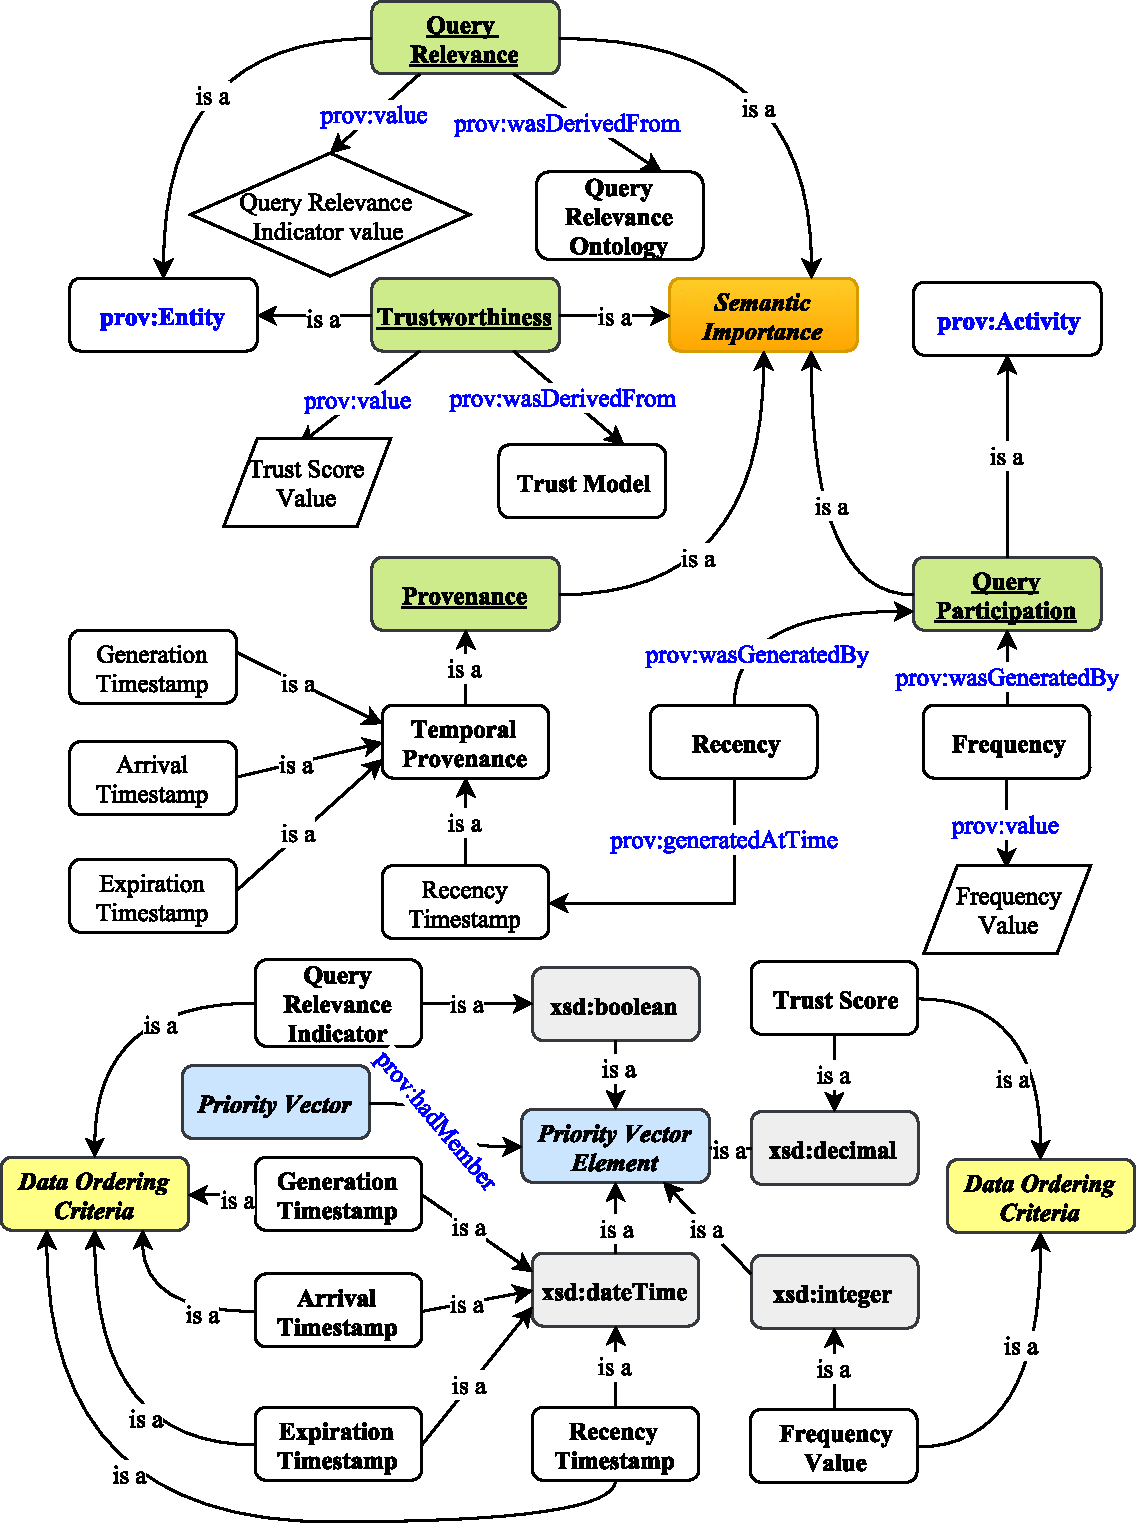
\includegraphics[width=5in]{img/6-sicr.pdf}
    \caption{\textbf{Semantic Importance Ontology}}
    \label{fig:6-sicr}
\end{figure}
%
\subsection{Connection to Stream Reasoning}
SIGenBench is designed in order to embrace both the state-of-the-art and popular stream reasoning techniques.
For instance, SIGenBench is compatible with different continuous query languages and report operational semantics. 
As \cite{dell2013correctness} mentions, the correctness of a stream reasoning engine is critically dependent upon the operational semantics. 
Since different stream reasoning systems can behave differently \cite{botan2010secret}, the benchmark systems aiming to measure the stream reasoning performance should be able to consider the differences in various built-in operational semantics.

SIGenBench decouples the operational semantics from stream reasoning engines.
For example, CSPARQL engine reports when the window is full, while a CQELS engine reports when the content in the window has changed (e.g. new data arrives). 
SIGenBench implements four different report policies, such that the users can specify which report policy and query language to use.
This loosens the strict one-to-one-pair of the report policy and query engine in most stream reasoning systems. 
That is to say, a CSPARQL query can work with ``on content change'' report policy, which increases the flexibility for prototyping and testing.

SIGenBench can naturally consume RDF streams.
RDF stream is also extended to carry more information such as explicit expiration timestamps and trust scores.
More details will be covered in the Implementation Section. 

SIGenBench works with two state of the art continuous query languages, namely CSPARQL and CQELS\footnote{Both CSPARQL and CQELS provide a stream reasoning engine and a continuous query language.}.
The reason to choose them is for their wide adoption in the stream reasoning applications \cite{dao2015towards} \cite{kolchin2014web} \cite{dejonghec} \cite{okure2013querying}.

SIGenBench is compatible with mainstream window operators including sliding and landmark window.
Chapter 3 has already covered the details of semantic extension for landmark windows.
It also mentions that the window definition for both CSPARQL and CQELS are only for sliding window.
SIGenBench aligns the these definitions for the landmark window. 
An exemplar logical window definition in CSPARQL is [RANGE 2s STEP 1s].
It defines the window size of 2 seconds, and step of 1 second. 
SIGenBench uses the same expression to initialize a logical lower-bounded landmark window as follows: 
the initial window size is 2 seconds worth of data items; its upper-bound moves per 1 second to consume the next 1 second worth of data items. 
%
\section{Benchmark}
The primary goal of the benchmark system in SIGenBench is to provide detailed empirical evidence for the deployment of various window management strategies supported by semantic importance.
SIGenBench is able to simulate a various of stream reasoning scenarios, thanks to the default streaming data generator, which provides flexible test beds for window management strategies.
The Evaluation Section will cover all the details.
It is worth mentioning that SIGenBench does not focus on benchmarking stream reasoning applications as a whole.
For such benchmark systems please refer to \cite{dell2013correctness} \cite{ali2015citybench} \cite{tommasini2015heaven} and \cite{benchmarkdemo}.
%
\section{Implementation}
SIGenBench is implemented based on SSRA, backed by Stardog triple-store.
It is written in Java and accepts command line arguments to configure one experiment. 
It outputs the results in real time, provides summary logs and performance evaluation.
This section highlights some core components of SIGenBench. 
%
\subsection{Window}
SIGenBench has 4 different built-in windows, including sliding logical window, sliding physical window, landmark logical window, and landmark physical window. 
A logical window has a size and a step that are both in temporal units (such as second, minute etc).
A physical window has a size and a step in terms of the number of data items. 
Sliding windows are commonly used windows in most stream reasoning systems. 
Landmark windows extend sliding windows by fixing the lower bound while allowing the upper bound proceeds.
Four aforementioned window report operational semantics are supported.
Please refer to Chapter 3 for all the details. 
Table \ref{tab:6-wc} lists the parameters to configure a window in SIGenBench

\begin{table}[!htbp]
	\centering
    \caption{\textbf{Window Configuration}}
    \label{tab:6-wc}
    \begin{tabular}{|c||l|l|} \hline
    parameter & \multicolumn{1}{c|}{option} & \multicolumn{1}{c|}{annotation} \\ \hhline{|=#=|=|}
    wt & \makecell[l]{sliding \\ landmark} & sliding or landmark window \\ \hline
    ut & \makecell[l]{logical \\ physical} & logical or physical window \\ \hline
    qt & \makecell[l]{CSPARQL \\ CQELS} & CSPARQL or CQELS query language \\ \hline
    opr & \makecell[l]{onWindowClose \\ onContentChange \\ nonEmptyContent \\ periodic} & report policy \\ \hline 
    stgy & strategies in Table \ref{tab:6-26s} & window management strategy \\ \hline
    \end{tabular}
\end{table}
%
\begin{table}[!htbp]
	\centering
    \caption{\textbf{SIGenBench Built-in Window Management Strategies}}
    \label{tab:6-26s}
    \begin{tabular}{|c||l|l|} \hline
         \# & \multicolumn{1}{c|}{Strategy Name} & \multicolumn{1}{c|}{Semantic Importance Priority Vector} \\ \hhline{|=#=|=|}
         1 & FIFO & $[\tau_{a}]$ \\ \hline
         2 & QR-FI-FO & $[qrf, \tau_{a}]$ \\ \hline 
         3 & Trust-FI-FO & $[t^{tm}_{s}, \tau_{a}]$ \\ \hline
         4 & FE-FO & $[\tau_{e}]$ \\ \hline
         5 & QR-FE-FO & $[qrf, \tau_{e}]$ \\ \hline
         6 & LFU-FO & $[f_{qp}]$ \\ \hline
         7 & QR-LFU-FO & $[qrf, f_{qp}]$ \\ \hline
         8 & LRU-FO & $[\tau_{qp}]$ \\ \hline
         9 & QR-LRU-FO & $[qrf, \tau_{qp}]$ \\ \hline
         10 & Trust-FO & $[t^{tm}_{s}]$ \\ \hline 
         11 & QR-Trust-FO & $[qrf, t^{tm}_{s}]$ \\ \hline 
         12 & QR-Trust-FI-FO & $[qrf, t^{tm}_{s}, \tau_{a}]$ \\ \hline
         13 & FE-FI-FO & $[\tau_{e}, \tau_{a}]$ \\ \hline
         14 & QR-FE-FI-FO & $[qrf, \tau_{e}, \tau_{a}]$ \\ \hline
         15 & FE-LFU-FO & $[\tau_{e}, f_{qp}]$ \\ \hline
         16 & QR-FE-LFU-FO & $[qrf, \tau_{e}, f_{qp}]$ \\ \hline
         17 & FE-LRU-FO & $[\tau_{e}, \tau_{qp}]$ \\ \hline
         18 & QR-FE-LRU-FO & $[qrf, \tau_{e}, \tau_{qp}]$ \\ \hline
         19 & FE-LFU-FI-FO & $[\tau_{e}, f_{qp}, \tau_{a}]$ \\ \hline
         20 & QR-FE-LFU-FI-FO & $[qrf, \tau_{e}, f_{qp}, \tau_{a}]$ \\ \hline
         21 & FE-LRU-FI-FO & $[\tau_{e}, \tau_{qp}, \tau_{a}]$ \\ \hline
         22 & QR-FE-LRU-FI-FO & $[qrf, \tau_{e}, \tau_{qp}, \tau_{a}]$ \\ \hline
         23 & Trust-FE-LFU-FI-FO & $[t^{tm}_{s}, \tau_{e}, f_{qp}, \tau_{a}]$ \\ \hline
         24 & QR-Trust-FE-LFU-FI-FO & $[qrf, t^{tm}_{s}, \tau_{e}, f_{qp}, \tau_{a}]$ \\ \hline
         25 & Trust-FE-LRU-FI-FO & $[t^{tm}_{s}, \tau_{e}, \tau_{qp}, \tau_{a}]$ \\ \hline
         26 & QR-Trust-FE-LRU-FI-FO & $[qrf, t^{tm}_{s}, \tau_{e}, \tau_{qp}, \tau_{a}]$ \\ \hline    
    \end{tabular}
\end{table}
\subsection{Window Management Strategy}
Semantic importance is the core contribution of this dissertation.
It also enables various window management strategies.
Currently, SIGenBench features 26 built-in strategies, as shown in Table \ref{tab:6-26s}.
This table also includes the priority vectors, which can indicate the semantic importance aspects used in one strategy. 
For example, FIFO manages data like a queue, and data is ranked by the arrival timestamps ($\tau_{a}$). 
A simple TRUST strategy is composed with a single trust score $t^{tm}_{s}$, which neglects all the temporal information associated with the data. 
There are certainly more compound strategies such as QR-Trust-FE-LRU-FIFO. 
A more compound strategy does not necessarily imply its better performance.
What the strategies' performance is dependent upon involves a list of factors, such as use case requirements, streaming data traits, the knowledge encoded in the ontology, as well as the efficiency of the processing machines, etc.
The performance can only be discussed after SIGenBench is deployed, is fed with streaming data and generates benchmark results. 
%
\subsection{Query}
SIGenBench takes both CSPARQL and CQELS query languages. 
This is made possible because SIGenBench leverages CSPARQL and CQELS engines' query parsers.
A parser splits a continuous query into two parts: a dynamic part with a stream and window definition, and a static part of a standard SPARQL query. 
Listing 6.1 shows an example of CSPARQL query, which defines the stream with ``FROM STREAM'' keyword, and the window with the argument of [RANGE 1s STEP 1s].
This indicates that the window size and step should be both 1 second.
Listing 6.2 shows a CQELS query that contains the window definition as [RANGE 2s SLIDE 2s].
It defines both the window size and step as 2 seconds.
Both queries can be parsed by their dedicated parsers into a standard SPARQL query shown in Listing 6.3.

\begin{lstlisting}[caption={\textbf{CSPARQL Query Example}},basicstyle=\small]
REGISTER QUERY test AS
PREFIX rdf: <http://www.w3.org/1999/02/22-rdf-syntax-ns#>
PREFIX ub: <http://swat.cse.lehigh.edu/onto/univ-bench.owl#>
SELECT ?s
FROM STREAM <http://ex.org/streams/test> [RANGE 1s STEP 1s]
WHERE {	
	?s rdf:type ub:Chair.
}
\end{lstlisting}

\begin{lstlisting}[caption={\textbf{CQELS Query Example}},basicstyle=\small]
PREFIX rdf: <http://www.w3.org/1999/02/22-rdf-syntax-ns#>
PREFIX ub: <http://swat.cse.lehigh.edu/onto/univ-bench.owl#>
SELECT ?s 
WHERE { 
	STREAM <http://ex.org/streams/test> [RANGE 2s SLIDE 2s] 
	{ 
    	?s rdf:type ub:Chair . 
    } 
}
\end{lstlisting}

\begin{lstlisting}[ caption={\textbf{Parsed Standard SPARQL Query}},basicstyle=\small]
PREFIX rdf: <http://www.w3.org/1999/02/22-rdf-syntax-ns#>
PREFIX ub: <http://swat.cse.lehigh.edu/onto/univ-bench.owl#>
SELECT ?s
WHERE {	
	?s rdf:type ub:Chair.
}
\end{lstlisting}
%
\subsection{Data Stream}
SIGenBench is naturally compatible with RDF streams in basic or extended formats.
A basic RDF stream format is $<\rho, \tau>$.
In an extended format, for example, the RDF stream with graph IDs can be expressed as $<\rho, g, \tau_{a}>$, where $g$ indicates the graph ID. 
This graph ID can contain information of the streaming source, or a dedicated ID for the specific data. 
$\tau_{a}$ represents the arrival timestamp. 
RDF stream format can be further extended as $<\rho, g, \tau_{a}, \tau_{e}, t^{tm}_{s}>$, where $\tau_{e}$ denotes the expiration timestamp, and $t^{tm}_{s}$ denotes the trust-score.
The expiration timestamp can be assigned by either the streaming source or the processing engine.
The period between the arrival and expiration timestamp is the data's time-to-live. 
The trust score can be assigned either by the system or the streaming source, indicating the trust level of such data. 

\textcolor{red}{
SIGenBench can accept either user specified data or a synthesized streaming data.
The synthesized streaming data is derived from LUBM datasets \cite{guo2005lubm}. 
\cite{DBLP:conf/semweb/NguyenS13} generates RDF streams using LUBM datasets.
Work like \cite{tommasini2015heaven} also uses LUBM dataset for the stream reasoning benchmark system.
The streaming data generator is inspired by these work. 
Our generator not only can generate single timestamped data streams such as the mentioned work does, but also can generate data stream with a valid period, graph ID, and trust score.
These information will be used for data processing in SIGenBench.
}

A simulated streaming data is generated by considering 5 dimensions, including streaming mode, streaming rate, expiration timestamp, trust score, and the amount of data (lubm). 
Table \ref{tab:6-sdgc} summarizes the parameters to configure the default streaming data.

\begin{table}[!htbp]
	\centering
    \caption{\textbf{Streaming Data Generator Configuration}}
    \label{tab:6-sdgc}
    \begin{tabular}{|c||l|l|} \hline
    parameter & \multicolumn{1}{c|}{option} & \multicolumn{1}{c|}{annotation} \\ \hhline{|=#=|=|}
    lubm & \makecell[l]{1: 100545 triples \\ 2: 230063 triples \\ 3: 337129 triples} & LUBM source data \\ \hline
    sm & \makecell[l]{c: constant mode \\ f: fluctuating mode} & stream mode \\ \hline
    sr & \makecell[l]{10000, 30000, 50000 \\ 70000, 90000} & \makecell[l]{constant rate in c mode, \\ peak rate in f mode} \\ \hline
    ets & \makecell[l]{1: quick expiration (1s to 3s) \\ 2: normal expiration (3s to 7s) \\ 3: slow expiration (7s to 10s) \\ 4: implicit expiration} & how quickly the data expires \\ \hline
    t & \makecell[l]{1: trust model 1 \\ 2: trust model 2 \\ 3: trust model 3 \\ 4: no trust model} & \makecell[l]{choose a trust model, append a \\trust score to each data item} \\ \hline
    \end{tabular}
\end{table}

Parameter ``lubm'' controls the total amount of data items in the synthesized data stream. 
Normally streaming data is considered to boundless, however, in order to complete the experiment, the synthesized data is set to be finite. 
There are two streaming modes, the constant mode (c mode) and the fluctuating mode (f mode).
C mode streams the data in a fixed data rate.
For example, in the soccer use case, all sensors stream data with a fixed frequency.
In c mode, the streaming rate indicates the actual data items streamed per second. 
F mode simulates bursts in streams with peaks and valleys. 
An example is the amount of traffic on a main road during the peak hours and off-peak hours. 
In f mode, the stream rate is actually the peak value. 
The probability of a peak value is 1/6, the probability of a valley (SIGenBench sets it as 0) is 1/6, the probability of an in-between value is 2/3. 
The rationales to set probabilities like this are from the traffic model. 
During 24 hours, rush hours are usually 4 hours (usually 7am to 9am and 4pm to 6pm).
From midnight to 4:00 am there are a few cars on the road; other time will usually have normal amount of traffic. 
Thus the peak probability is 4/24 = 1/6, ditto for others.
Streaming data can carry explicit or implicit data expiration stamps.
Data can expire fast, normally or slowly.
There three built-in trust models to assign trust scores for data items.

\begin{lstlisting}[caption={\textbf{Generated RDF Stream Example 1}},basicstyle=\tiny]
<http://www.Department2.University0.edu/AssistantProfessor0/Publication7> 
<http://swat.cse.lehigh.edu/onto/univ-bench.owl#publicationAuthor>
<http://www.Department2.University0.edu/GraduateStudent33> 
<http://tw.rpi.pnnl.org/sigenbench/graph0> 
11:24:05.679 11:24:08.679 0.7318180206732977
\end{lstlisting}

\begin{lstlisting}[caption={\textbf{Generated RDF Stream Example 2}},basicstyle=\tiny]
<http://www.Department5.University0.edu/FullProfessor4>
<http://www.w3.org/1999/02/22-rdf-syntax-ns#type>
<http://swat.cse.lehigh.edu/onto/univ-bench.owl#FullProfessor>
<http://tw.rpi.pnnl.org/sigenbench/graph32513> 11:24:08.930 11:24:11.930 9.557774771623334

<http://www.Department5.University0.edu/FullProfessor4>
<http://swat.cse.lehigh.edu/onto/univ-bench.owl#headOf>
<http://www.Department5.University0.edu>
<http://tw.rpi.pnnl.org/sigenbench/graph47329> 11:24:10.411 11:24:12.411 9.5384934592904
\end{lstlisting}

\begin{lstlisting}[caption={\textbf{Generated RDF Stream Example 3}},basicstyle=\tiny]
<http://www.Department10.University0.edu/FullProfessor5>
<http://swat.cse.lehigh.edu/onto/univ-bench.owl#headOf>
<http://www.Department10.University0.edu>
<http://tw.rpi.pnnl.org/sigenbench/graph56649> 11:24:11.343 11:24:12.343 9.050994502744377

<http://www.Department10.University0.edu/FullProfessor5>
<http://www.w3.org/1999/02/22-rdf-syntax-ns#type>
<http://swat.cse.lehigh.edu/onto/univ-bench.owl#FullProfessor>
<http://tw.rpi.pnnl.org/sigenbench/graph72474> 11:24:12.926 11:24:14.926 9.015205125311985
\end{lstlisting}

The data generator shuffles the LUBM data, so that the data is randomly distributed.
Listing 6.4 shows an example of a streaming data item in $<\rho, g, \tau_{a}, \tau_{e}, t^{tm}_{s}>$ format.
However, shuffling will possibly lead to no ground truth. 
Consider Examples in Listing 6.5 and 6.6. 
In Listing 6.5, graph32513 and graph47329 are both about $<$\url{http://www.Department5.University0.edu/FullProfessor4}$>$. 
They have an overlapping time period from 11:24:10.411 to 11:24:11.930.
Thus they can generate the result that $<$\url{http://www.Department5.University0.edu/FullProfessor4}$>$ is a \textbf{ub:Chair}.
However, Listing 6.6 provides another data where graph47329 and graph56649 do not have an overlapping period, thus $<$\url{http://www.Department5.University0.edu/FullProfessor4}$>$ will not be inferred as \textbf{ub:Chair}.
These two examples are also corresponding to the early eviction and early expiration problems introduced in previous sections. 
If not enough ground truth is produced, the generator will run again till enough ground truth is produced.

%
\subsection{Ontology}
SIGenBench can work with all ontologies encoded in OWL.
Just like other benchmarks \cite{dell2013correctness} \cite{ali2015citybench}, by default SIGenBench comes with a test ontology derived from LUBM \cite{guo2005lubm}.
This ontology itself contains detailed information about the updates that had been made and related rationales. 
However, it is worth mentioning this: a new class, the subclass of \textbf{Thing}, named \textbf{ub:DepartmentHead} is added, and defined as (\textit{ub:headOf some} \textbf{ub:Department)}. 
It is added to facilitate the query relaxation on \textbf{ub:Chair}. 
Previously, \textbf{ub:Chair} is defined as (\textbf{ub:Person} \textit{and} (\textit{ub:headOf some} \textbf{ub:Department})). 
There is an anonymous class that fails schema-based query relaxation due to blank nodes. 
In order to avoid this, \textbf{ub:DepartmentHead} is created and defined.
The reason not to include it under \textbf{ub:Person} or \textbf{ub:Professor} is to avoid any possible RDFS hierarchical reasoning. 
\textit{ub:headOf} is defined originally in LUBM without any domain or range, which means (\textit{ub:headOf some} \textbf{ub:Department}) will not entail any type.
This is also the reason not to include \textbf{ub:DepartmentHead} under \textbf{ub:Person} or \textbf{ub:Professor}.
All the experiments will be conducted upon this default ontology in this dissertation.
%
\subsection{Query Relaxation}
Query relaxation is a general research topic that deals with relaxing a query when no results are returned,via loosening the constraints in the query \cite{hurtado2008query} \cite{reddy2010efficient} \cite{viswanathan2016pragmatic}.
In SIGenBench, a schema-based query relaxation method is used.
The target query will be relaxed according to the window management strategy and system output.
The classes in the target query will be replaced by their super classes in a relaxed query that will run again to collect any results. 
For instance, if the SPARQL query in Listing 6.3 cannot generate results, it can be relaxed according to the schema in the background ontology \textbf{ub:Chair} $\equiv$ (\textbf{ub:DepartmentHead} \textit{and} \textbf{ub:Person}).
Listing 6.7, and 6.8 show two relaxed queries.

The discussion of the performance of query relaxation in general is out of the realm of this dissertation. 
The purpose is to leverage some query relaxation techniques that can work well with SIGenBench. 
A future work would be to modularize the query relaxation component and allow users to specify they relaxation algorithms to use.

\begin{lstlisting}[ caption={\textbf{Relaxed Query 1}},basicstyle=\small]
PREFIX rdf: <http://www.w3.org/1999/02/22-rdf-syntax-ns#>
PREFIX ub: <http://swat.cse.lehigh.edu/onto/univ-bench.owl#>
SELECT ?s
WHERE {	?s rdf:type ub:DepartmentHead.}
\end{lstlisting}

\begin{lstlisting}[ caption={\textbf{Relaxed Query 2}},basicstyle=\small]
PREFIX rdf: <http://www.w3.org/1999/02/22-rdf-syntax-ns#>
PREFIX ub: <http://swat.cse.lehigh.edu/onto/univ-bench.owl#>
SELECT ?s
WHERE {	?s rdf:type ub:Person.}
\end{lstlisting}
%
\section{Evaluation}
This section provides detailed benchmark results.
The analysis and discussions are focused on three main categories: semantic importance, window, and streaming data.
All experiments are run on a Windows 7 machine with eight-core Inter(R) Core(TM) i7-3720QM CPU @ 2.6GHZ, 8GB RAM, and a SSD. 
%
\subsection{Semantic Importance}
Each aspect of semantic importance has been benchmarked in multiple experiments so as to reveal its influence on the system performance. 
%
\subsubsection{Query Relevance}
Query relevance is an important aspect, as it brings the domain into computation.
It features a filter query and an optional query relevance ontology that encodes the knowledge of data-query relevance.
The purpose to propose query relevance is to enable the system's identification of the relevant information to keep. 
By plugging a query relevance filter in front of the window, irrelevant data will be filtered out.

The hypothesis is that query relevance will help save system response time, which has been validated from the results at Table \ref{tab:6-qrp}. 
The benefits brought by query relevance are augmented as system precision, memory consumption and throughput have all been improved. 
However, query relevance ontology is not the only factor to decide the performance. 
The actual filtering query also has the power to influence the system performance. 
In order to show this, this thesis has used three different queries as in Listing 6.9, 6.10, and 6.11.
Listing 6.9 shows a filtering query that keeps only the necessary data items.
Listing 6.10 shows a filtering query that keeps both all the necessary data items and some unnecessary data items.
Listing 6.11 shows a filtering query that fails to capture all necessary data items.

\begin{lstlisting}[caption={\textbf{Query Relevance Filtering Query 1}},basicstyle=\small]
PREFIX ub: <http://swat.cse.lehigh.edu/onto/univ-bench.owl#>
SELECT ?g
WHERE {
    GRAPH ?g {
        {?s rdf:type ub:FullProfessor}
        UNION
    	{?s ub:headOf ?o}  
    }
}
\end{lstlisting}

In order to determine if a person is a \textbf{ub:DepartmentHead}, according to the background ontology, two data items are needed: this person has to be both \textbf{ub:FullProfessor} and \textit{ub:headOf} something.
Technically, data items that do not have these two information are irrelevant, thus can be filtered out. 
Filter query in Listing 6.9 will only let the system to keep the relevant data.
Typically, query relevance filter query can have two ways to filter the data: use some SPARQL Delete or Drop argument in the filter query itself to get rid of the irrelevant data, or use SPARQL graph pattern match to query the relevant data to keep. 
This dissertation adopts the second way, because the implementation is easier and faster.

\begin{lstlisting}[caption={\textbf{Query Relevance Filtering Query 2}},basicstyle=\small]
PREFIX ub: <http://swat.cse.lehigh.edu/onto/univ-bench.owl#>
SELECT ?g
WHERE { 
    GRAPH ?g {
        {?s rdf:type ?type}
        UNION 
        {?s ub:headOf ?o}  
    }
}
\end{lstlisting}

This query introduces some irrelevant data and sees it as relevant data, from the argument of ``?s rdf:type ?type''.
This query will still be able to filter out some amount of the irrelevant data which can improve system response time.
It is likely to use this type of filter query in real world use case though, because the knowledge about the streaming data and target query can be limited. 
However, the goal is to filter out as much irrelevant data as possible so that the system performance can be improved.
As what will be shown later, streaming data rate also influences the system response time. 
If the data rate is big, it will take longer time to process the filtering, which can hurt the overall usefulness of system.

Listing 6.11 shows a filtering query where the relevant data of \textbf{ub:FullProfessor} is filtered out.
Predictably, the target query will not provide any results. 
In general applications, one should avoid this type of query to be deployed in the system. 
Table \ref{tab:6-fqqi} summarizes the impacts of the above three queries. 

\begin{lstlisting}[caption={\textbf{Query Relevance Filtering Query 3}},basicstyle=\small]
PREFIX ub: <http://swat.cse.lehigh.edu/onto/univ-bench.owl#>
SELECT ?g
WHERE {
    GRAPH ?g {
    	{?s ub:headOf ?o}  
    }
}
\end{lstlisting}

\begin{table}[!htbp]
	\centering
    \caption{\textbf{Query Relevance Experiments Setup}}
    \label{tab:6-qres} 
    \begin{tabular}{|c|l|} \hline
    \multicolumn{2}{|c|}{\textbf{experiment configuration}} \\ \hline
    window & \makecell[l]{logical lower-bounded landmark window \\ initial window size = 1s, 2s and 3s worth of data items \\ window step = 1s worth of data items \\ report policy = onWindowClose \\ all 26 strategies in Table \ref{tab:6-26s}} \\ \hline
    data stream & \makecell[l]{lubm = 1 \\ sm = c (constant mode) \\ sr = 10000 data items/second \\ ets = 1 quick expiration (1s to 3s) \\ t = 3 (trust model 3)} \\ \hline 
    query & CSPARQL query \\ \hline
    \multicolumn{2}{|c|}{\textbf{experiment variable}} \\ \hline
    QR filter & \makecell[l]{Listing 6.9, 6.10, and 6.11} \\ \hline
    \end{tabular}
\end{table}

Table \ref{tab:6-qres} shows the experiments setup and variable.
The reason to choose 1s to 3s for window sizes is because of the quick data expiration. 
Since the data will expire after 3 seconds, it is pointless to make the window size longer than 3 seconds since data will expire within the window.
In the following section, we will see that a bigger window size will impact the precision adversely when data quickly expires. 

\begin{table}[!htbp]
	\centering
    \caption{\textbf{Query Relevance Filter Query 1 Performance}}
    \label{tab:6-qrp}
    \begin{tabular}{|l||c|c|c|c|} \hline
         \multicolumn{1}{|c||}{strategy} & memory & response time & precision & throughput \\ \hhline{|=#=|=|=|=|}
FIFO             & 11202.70 & 3363.00 & 0.08 & 2922.16\\ \hline 
FE-FO             & 11748.26 & 3207.94 & 0.17 & 3039.05\\ \hline 
LFU-FO            & 11265.96 & 2442.07 & 0.17 & 1657.71\\ \hline 
LRU-FO            & 11265.96 & 2328.31 & 0.17 & 1647.76\\ \hline 
FE-FI-FO           & 11791.24 & 2947.67 & 0.17 & 3282.85\\ \hline 
FE-LRU-FO          & 11699.40 & 2937.96 & 0.17 & 3343.14\\ \hline 
Trust-FO          & 1420.12 & 122.62 & 1 & 52088.41\\ \hline 
FE-LFU-FO          & 11699.40 & 3184.02 & 0.17 & 3184.86\\ \hline 
Trust-FI-FO        & 3371.94 & 178.03 & 1 & 41686.66\\ \hline 
FE-LRU-FI-FO        & 11670.60 & 3207.79 & 0.17 & 3086.81\\ \hline 
FE-LFU-FI-FO        & 11699.22 & 3033.25 & 0.17 & 3262.87\\ \hline 
Trust-FE-LRU-FI-FO   & 2860.00 & 174.58 & 1 & 64967.53\\ \hline 
Trust-FE-LFU-FI-FO   & 2128.82 & 162.76 & 1 & 69675.84\\ \hhline{|=#=|=|=|=|}
QR-FI-FO           & 18.98 & 372.07 & 1 & 31721.05\\ \hline 
QR-FE-FO           & 27.35 & 330.27 & 1 & 33840.54\\ \hline 
QR-LFU-FO          & 19.82 & 270.78 & 1 & 34113.49\\ \hline 
QR-LRU-FO          & 19.82 & 263.19 & 1 & 34980.15\\ \hline 
QR-FE-FI-FO         & 28.94 & 250.74 & 1 & 41555.22\\ \hline 
QR-FE-LFU-FO        & 28.37 & 260.30 & 1 & 40068.32\\ \hline 
QR-FE-LRU-FO        & 28.22 & 268.26 & 1 & 38881.49\\ \hline 
QR-Trust-FO        & 82.13 & 255.51 & 1 & 29858.80\\ \hline 
QR-Trust-FI-FO      & 82.13 & 252.80 & 1 & 30383.74\\ \hline 
QR-FE-LFU-FI-FO      & 28.32 & 263.55 & 1 & 39400.00\\ \hline 
QR-FE-LRU-FI-FO      & 28.29 & 263.65 & 1 & 39430.94\\ \hline 
QR-Trust-FE-LFU-FI-FO & 28.33 & 261.36 & 1 & 39796.71\\ \hline 
QR-Trust-FE-LRU-FI-FO & 27.94 & 277.98 & 1 & 37607.35\\ \hline 
    \end{tabular}
    \begin{tablenotes}
 		\item memory unit: number of data items
 		\item response time unit: ms
 		\item throughput unit: data items/second
    \end{tablenotes}
\end{table}

\begin{table}[!htbp]
	\centering
    \caption{\textbf{Different Filter Query Experimental Results}}
    \label{tab:6-fqqi}
    \begin{tabular}{|c||c|c|c|c|} \hline
    query & ave. memory & ave. response time & ave. precision & ave. throughput \\ \hhline{|=#=|=|=|=|}
    none & 8755.66 & 2099.23 & 0.42 & 19526.59 \\ \hline
    Query 1 & 34.51 & 276.19 & 1.00 & 36279.83\\ \hline
    Query 2 & 1882.19 & 739.97 & 0.92 & 19140.17\\ \hline
    Query 3 & 5.62 & 250.33 & 0 & 41018.93\\ \hline
    \end{tabular}
    \begin{tablenotes}
 		\item memory unit: number of data items
 		\item response time unit: ms
 		\item throughput unit: data items/second
    \end{tablenotes}
\end{table}

Table \ref{tab:6-qrp} shows the system performance under all 26 built-in strategies with query relevance filter query 1.
It is obvious that QR aspect alone can improve system performance significantly. 
For example, for FIFO and QR-FI-FO, the memory consumption is 11202.70 vs 18.78, which is almost 600x improvement. 
Table \ref{tab:6-fqqi} shows that compared with all non-QR strategies, on average Query 1 can reduce memory consumption by 253.71 times, improve response time by 7.6 times, improve precision by 2.38 times, and improve throughput by 1.86 times. 
With a reduced memory consumption, the system is able to be deployed in a resource-constrained environment, or an environment that can allocate less resource to store streaming data. 
Since less data is in the window, the overall system will respond way more quickly, which can also increase the system throughput. 
In the good QR example, the system precision is improved because of only the necessary data is preserved. 

For all non-QR strategies, FIFO has the worst precision, which shows that the temporal silent assumption generally does not work well.
Trust related strategies show a superior performance in precision and throughput. 
In fact, non-QR trust related strategies have the best throughput of all.
This is because of the fast execution of the trust comparison operation.
Basically, all data will be ranked by their trust score first under Trust related strategies. 
\textcolor{red}{
Unlike query relevance where the filter query has to be executed, data filtered by trust score will only take linear time, which is way more faster.
That explains why trustworthiness does not grow as fast as others in terms of response time.
}
Another part of reason for non-QR trust related strategies' high precision is that the data is generated with Trust Model 3. 
For details about the trust mode, please refer to the trustworthiness section below. 

All QR related strategies have good precision of 1 and relatively high throughputs. 
Note that the streaming data has a constant rate of 10000 data items per second. 
All QR related strategies has a throughput bigger than 10000, which means that they are able to process that amount of data within one second.
An eligible stream reasoning system should at least finish processing the data in the window before window consumes next round of data so as to avoid data congestion or any delay. 
The average response time of all QR-related strategies with good QR filter is 276.19 ms and is smaller than window step, while non-QR strategies has 2099.23 ms. 
This means non-QR strategies will need more than 2 seconds to process 10000 data items, which makes the system not usable at all. 
The only exception in non-QR strategies is those non-QR Trust related strategies. 

Table \ref{tab:6-fqqi} shows the impacts from different filter query influences. 
Query 2's impact is called ``under filter impact''; Query 3's filter query impact is called ``over filter impact''.
In the under filter situation, more data are kept in the window thus system response time is slower than good QR's, but faster than the window step thus the precision is still good.
Its throughput drops but still bigger than the stream rate thus capable of processing data stream. 
Nonetheless, in the over filter situation, not only all irrelevant data, but also some relevant data is filtered out, resulting in a very small memory consumption. 
The precision drops to 0, which means the system is barely useful.
The experimental results illustrate that query relevance filter queries/ontology does have impacts on system performance, and it is critical to deploy good quality query relevance in the system for better performance. 
%
\subsubsection{Temporal Provenance}
Temporal features are RDF streams' inherent nature. 
Stream reasoning applications should be able to keep a close track of the validity of all RDF stream items, and evict them if invalid within the window.
Most stream reasoning applications use arrival or generation timestamps.
Chapter 2 has already analyzed the impacts of these two.
The recency timestamp will be evaluated in query participation section.

This section aims to show how system performance can be influenced by considering data expiration.
The valid period or time-to-live of one data item can be obtained by subtracting its arrival timestamp from its expiration timestamp, assuming that data carries explicit expiration timestamps.
If data only carries arrival timestamps, then its expiration timestamps will be assigned by window management strategies. 
If data expires quickly, the challenge of timely processing will be increasing, as the delay tolerance will be decreasing. 
Table \ref{tab:6-dees} shows the experiments setup.

\begin{table}[!htbp]
	\centering
    \caption{\textbf{Data Expiration Experiments Setup}}
    \label{tab:6-dees}
    \begin{tabular}{|c|l|} \hline
    \multicolumn{2}{|c|}{\textbf{experiment configuration}} \\ \hline
    window & \makecell[l]{logical lower-bounded landmark window \\ initial window size = 1s, 2s, and 3s worth of data items \\ window step = 1s worth of data items \\ report policy = onWindowClose} \\ \hline
    data stream & \makecell[l]{lubm = 1 \\ sm = c (constant) \\ sr = 10000 data items/second \\ t = 3 (trust model 3)} \\ \hline
    query & \makecell[l]{CSPARQL target query \\ query relevance filter query 1 as in Listing 6.9} \\ \hline
    \multicolumn{2}{|c|}{\textbf{experiment variable}} \\ \hline
    data expire & \makecell[l]{ets = 1 quick expiration (1s to 3s) \\ ets = 2 normal expiration (3s to 7s) \\ ets = 3 slow expiration (7s to 10s)} \\ \hline
    strategy & \makecell[l]{FIFO, FE-FO, FE-FI-FO} \\ \hline
    \end{tabular}
\end{table}

\begin{table}[!htbp]
\centering
\caption{\textbf{Data Expiration Experimental Results}}
\label{tab:6-dei}
\begin{tabular}{|c||c||c|c|c|c|}
\hline
expiration & strategy & memory & response time & precision & throughput \\ \hhline{|=#=#=|=|=|=|}
\multirow{3}{*}{quick} & FIFO & 11202.70 & 3363.00 & 0.08 & 2922.16 \\ \cline{2-6} 
 					  & FE-FO & 11748.26 & 3207.94 & 0.17 & 3039.05 \\ \cline{2-6} 
 					  & FE-FI-FO & 11791.24 & 2947.67 & 0.17 & 3282.85 \\ \hhline{|=#=#=|=|=|=|}
\multirow{3}{*}{normal} & FIFO & 11202.70 & 2672.81 & 0.86 & 3819.41 \\ \cline{2-6} 
 						& FE-FO & 14415.96 & 2930.00 & 0.79 & 3335.24 \\ \cline{2-6} 
 						& FE-FI-FO & 14214.79 & 2850.27 & 0.79 & 3307.16 \\ \hhline{|=#=#=|=|=|=|}
\multirow{3}{*}{slow} & FIFO & 11202.70 & 2552.73 & 0.95 & 3908.22\\ \cline{2-6} 
					  & FE-FO & 18308.39 & 2647.01 & 0.92 & 3099.00 \\ \cline{2-6} 
 					  & FE-FI-FO & 18381.85 & 2607.76 & 0.92 & 3104.45 \\ \hline
\end{tabular}
	\begin{tablenotes}
 		\item memory unit: number of data items
 		\item response time unit: ms
 		\item throughput unit: data items/second
    \end{tablenotes}
\end{table}

In the default data generator, the expiration timestamps are randomly assigned but follow a uniform distribution.
For example, in a quick expiration scenario, the probability of a data item to expire within 1s, 2s or 3s is equally 1/3.
One data items' expiration timestamp is its arrival timestamp plus its valid period.
This is critical to explain the performance differences for three strategies in Table \ref{tab:6-dei}.
In either data expiration scenario, all the strategies have similar response time and throughput. 
The obvious differences are precision and memory consumption. 

In the quick expiration scenario, all three strategies have poor precision, and FIFO is the worst. 
All three strategies' response time is almost 3 seconds, which means none of them is able to keep up with data expiration. 
However, as data gradually expires slowly, the precision increases significantly.
Response time has not changed much, but data time-to-live is prolonged, which allows finishing processing before data expiration and improves precision. 
However, no matter how good the precision looks, the fact that all three strategies are not able to finish processing before window moves makes them not applicable at all. 
In order to boost the response time, QR aspect is recommended.
Table \ref{tab:6-qrp} shows that under quick expiration scenario, QR strategies show faster response time and higher precision than their non-QR counterparts. 

Table \ref{tab:6-dei} also shows that the memory consumption for FE-FO and FE-FI-FO increases as data expires slowly. 
This can be explained by the uniform distribution of data expiration as well. 
Consider the quick expiration scenario: 
FIFO is blind about the data expiration, thus each time it will evict the oldest 1 second worth of data items.
However, generally only 1/3 of the oldest 1s worth of data will expire, thus the amount to evict in FE-FO and FE-FI-FO is always less than FIFO, resulting more data in the window.
More data in the window means more time to process them, thus FIFO runs slightly faster than the other two as data expires slowly.
%
\subsubsection{Query Participation}
Query participation is essentially the statistics of data-query interaction.
This includes query participation frequency ($f_{qp}$), and query participation recency ($\tau_{qp}$).
The idea is to collect either the frequency or the recency of the data that takes part in the query when results are given.
Technically, in order to collect such statistics, reasoning explanation is required. 
Reasoning explanation is able to trace back to the query and reasoning process, and figure out the exact data items that contribute to the results.
Stardog provides such functionality. 
However, if the query result returns empty, query relaxation will be performed. 
Basically, if the query needs to be answered with multiple data items which can be arbitrarily apart, the system should be able not only to identify these partial data items, collect them and wait for all of them to arrive in the window, but also needs to keep an eye on the validity of the data. 
Table \ref{tab:6-qpes} shows the experiments setup. 

\begin{table}[!htbp]
	\centering
    \caption{\textbf{\textbf{Query Participation Experiments Setup}}}
    \label{tab:6-qpes}
    \begin{tabular}{|c|l|} \hline
    \multicolumn{2}{|c|}{\textbf{experiment configuration}} \\ \hline
    window & \makecell[l]{logical lower-bounded landmark window \\ initial window size = 1s, 2s, and 3s worth of data items \\ window step = 1s worth of data items \\ report policy = onWindowClose} \\ \hline
    data stream & \makecell[l]{lubm = 1 \\ sm = c (constant) \\ sr = 10000 data items/second \\ t = 3 (trust model 3)} \\ \hline
    query & \makecell[l]{CSPARQL target query \\ query relevance filter query 1 as in Listing 6.9} \\ \hline
    \multicolumn{2}{|c|}{\textbf{experiment variable}} \\ \hline
    data expiration & \makecell[l]{ets = 1 quick expiration (1s to 3s) \\ ets = 2 normal expiration (3s to 7s) \\ ets = 3 slow expiration (7s to 10s) \\ ets = 4 implicit} \\ \hline
    strategy & \makecell[l]{FIFO, LFU-FO, LRU-FO} \\ \hline
    \end{tabular}
\end{table}

\begin{table}[!htbp]
	\centering
    \caption{\textbf{\textbf{Query Participation Experimental Results}}}
    \label{tab:6-qpp}
    \begin{tabular}{|c||c||c|c|c|c|} \hline
    expiration & strategy & memory & response time & precision & throughput \\ \hhline{|=#=#=|=|=|=|}
    \multirow{3}{*}{quick} & FIFO   & 11202.70 & 3363.00 & 0.08 & 2922.16 \\ \cline{2-6} 
 					      & LRU-FO & 11265.96 & 2328.31 & 0.17 & 1647.76 \\ \cline{2-6} 
 					      & LFU-FO & 11265.96 & 2442.07 & 0.17 & 1657.71 \\ \hhline{|=#=#=|=|=|=|}
	\multirow{3}{*}{normal} & FIFO   & 11202.70 & 2421.43 & 0.88 & 4059.49 \\ \cline{2-6} 
 						    & LRU-FO & 11232.80 & 2066.55 & 0.79 & 1968.92 \\ \cline{2-6} 
 						    & LFU-FO & 11232.85 & 2084.09 & 0.79 & 1982.39 \\ \hhline{|=#=#=|=|=|=|}
	\multirow{3}{*}{slow} & FIFO & 11202.70   & 2473.60 & 1.00 & 4070.88 \\ \cline{2-6} 
					      & LRU-FO & 11219.41 & 2140.02 & 1.00 & 2272.06 \\ \cline{2-6} 
 					      & LFU-FO & 11219.41 & 2143.75 & 1.00 & 2252.67 \\ \hhline{|=#=#=|=|=|=|}
    \multirow{3}{*}{none} & FIFO & 10832.36 & 2482.13 & 1.00 & 3789.58 \\ \cline{2-6}
    					  & LRU-FO & 11217.14 & 2148.26 & 1.00 & 2231.22 \\ \cline{2-6}
                          & LFU-FO & 11217.14 & 2155.60 & 1.00 & 2230.48 \\ \hline
	\end{tabular}
    \begin{tablenotes}
 		\item memory unit: number of data items
 		\item response time unit: ms
 		\item throughput unit: data items/second
    \end{tablenotes}
\end{table}

Table \ref{tab:6-qpp} shows the experimental results. 
It can be seen that data expiration influences strategy precision most, which can be explained with the same rationales from temporal provenance. 
As data expires slowly, all strategies' precision increases. 
LFU-FO and LRU-FO has faster response time than FIFO, but smaller throughput. 
Generally speaking, query participation alone does not show an obvious improvements for overall system performance.
The results indicate that query participation is most useful when data expires fast.
Technically, none of the tested three strategies are applicable in stream reasoning settings due to their slow response time. 
However, if QR aspect is added as shown in Table \ref{tab:6-qrp}, query participation related strategies are able to run faster. 
In summary, the purpose of proposing query participation aspect is to make sure all the necessary data can be collected even though they are arbitrarily apart, with the premise that all data should be valid.
%
\subsubsection{Trustworthiness}
Trustworthiness of the streaming data is very helpful to enable data awareness. 
The trust model encodes the knowledge of whether and to what degree the data should be trusted.
This dissertation assumes that data trustworthiness is reduced into a numerical value to facilitate data ranking.
The trust score can be assigned by either the streaming source or the processing system using some trust models. 
Even though the trust models are not within the realm of this dissertation, it is worth pointing out that different trust models can affect the system performance. 

The default streaming data of SIGenBench comes with 3 different trust models, which is shown in Table \ref{tab:6-tme}.
The data items will be annotated with different trust scores by different models.
\textcolor{red}{
The trust score used in the model is ranging from 0 to 10, with 0 to be least trustworthy, and 10 to be the most trustworthy.
(a, b) in the Table \ref{tab:6-tme} indicates a range of the trust score. 
The trust score will be generated randomly within the range between a and b. 
These three trust models concentrates different kinds of the data. 
For example, Model 1 evaluates ResearchGroup to be the most trustworthy, and assign the trust score within the range of 8 to 10.
Model 2 evalutes FullProfessor, AssociateProfessor, and AssistantProfessor related data to be more trusted.
Model 3 trusts most the FullProfessor related data, and leaving the other data not very much trusted.
}
Table \ref{tab:6-tes} shows the experiment setup.

\begin{table}[!htbp]
	\centering
    \caption{\textbf{Trust Models Example}}
    \label{tab:6-tme}
    \begin{tabular}{|l||c|c|c|} \hline
    	& trust model 1 & trust model 2 & trust model 3 \\ \hline
     \multicolumn{1}{|c||}{related data} & \multicolumn{3}{c|}{trust score range} \\ \hhline{|=#=|=|=|}
     FullProfessor & (0, 1) & (5, 10) & (9, 10) \\ \hline
     AssociateProfessor & (4, 7) & (5, 10) & (0, 1) \\ \hline
     AssistantProfessor & (5, 9) & (5, 10) & (0, 1) \\ \hline
     Publication & (5, 10) & (0, 10) & (0, 1) \\ \hline
     ResearchGroup & (8, 10) & (0, 10) & (0, 1) \\ \hline
     Student & (0, 2) & (0, 10) & (0, 1) \\ \hline
     Course & (0, 1) & (0, 10) & (0, 1) \\ \hline
     others & (0, 10) & (0, 10) & (0, 1) \\ \hline    
    \end{tabular}
\end{table} 

\begin{table}[!htbp]
	\centering
    \caption{\textbf{Trustworthiness Experiments Setup}}
    \label{tab:6-tes}
    \begin{tabular}{|c|l|} \hline
    \multicolumn{2}{|c|}{\textbf{experiment configuration}} \\ \hline
    window & \makecell[l]{logical lowerbounded landmark window \\ initial window size = 1s, 2s, and 3s worth of data items \\ window step = 1s worth of data items \\ report policy = onWindowClose} \\ \hline
    data stream & \makecell[l]{lubm = 1 \\ sm = c (constant) \\ sr = 10000 data items/second \\ ets = 1 quick expiration (1s to 3s)} \\ \hline
    query & \makecell[l]{CSPARQL target query \\ query relevance filter query 1 as in Listing 6.9} \\ \hline
    \multicolumn{2}{|c|}{\textbf{experiment variable}} \\ \hline
    trust model & \makecell[l]{t = 1 (trust model 1) \\ t = 2 (trust model 2) \\ t = 3 (trust model 3)} \\ \hline
    strategy & FIFO, Trust-FO  \\ \hline
    \end{tabular}
\end{table}

\begin{table}[!htbp]
	\centering
    \caption{\textbf{Trustworthiness Experimental Results}}
    \label{tab:6-tp}
    \begin{tabular}{|c||c|c|c|c|c|} \hline
    trust model & strategy & memory & response time & precision & throughput \\ \hhline{|=#=|=|=|=|=|}
    \multirow{2}{*}{Model 1} & FIFO & 11202.70 & 2517.42 & 0 & 3900.14 \\ \cline{2-6} 
    						 & Trust-FO & 11544.25 & 500.62 & 0 & 24614.08 \\ \hhline{|=#=|=|=|=|=|}
    \multirow{2}{*}{Model 2} & FIFO & 11202.70 & 2369.23 & 0.17 & 4211.35 \\ \cline{2-6} 
    						 & Trust-FO & 22012.32 & 1448.05 & 0 & 6175.97 \\ \hhline{|=#=|=|=|=|=|}
    \multirow{2}{*}{Model 3} & FIFO & 11202.70 & 3363.00 & 0.08 & 2922.16 \\ \cline{2-6} 
    						 & Trust-FO & 1420.12 & 122.62 & 1.00 & 52088.41\\ \hline 
    \end{tabular}
    \begin{tablenotes}
 		\item memory unit: number of data items
 		\item response time unit: ms
 		\item throughput unit: data items/second
    \end{tablenotes}
\end{table}

Table \ref{tab:6-tp} obviously shows that different trust model can have different impacts for the system performance. 
The information needed to answer the target query is actually all about ``FullProfessor''.
This can be deducted from the target query in Listing 6.1 and RDF stream example in Listing 6.6.
Model 1 assigns the smallest trust score for ``FullProfessor'', which means that the necessary data will be evicted quickly in the window by Trust-FO strategy. 
Model 2 Trusts information about professors but other data can also have high trust scores.
Model 3 Trusts ``FullProfessor'' related data only.
In order to explain the performance, both the target query and the window management strategies should be considered. 
In fact, Trust-FO only does one thing: to keep the data with the most trust scores.
If the most trusted data contains all the necessary information to answer the query, it will get good result. 
If not, the precision will be bad. 
Model 3 consumes the least memory because the amount of data trusted in the stream is the smallest. 
Trust-FO always has a better response time and throughput over FIFO, but its precision performance is really dependent upon trust models. 
%
\subsection{RDF Stream}
Streaming data is heterogeneous in many ways. 
SIGenBench models RDF stream in two dimensions, the streaming rate and the streaming mode.
Streaming rate indicates how fast the streaming data flows. 
Streaming mode describes the behavior of the streaming data.
A constant mode example is related to the frequencies of the sensor that streams the data. 
In the soccer offside detection use case, sensors are streaming data in high but constant frequencies. 
However, not all of the data streams are constant, there are situations where the data streams can be fluctuating. 
In other situations, for example, the traffic in the main street at rush hours will be significantly busier than non-rush hours, so the data streams to the traffic monitor systems will contain peaks and valleys.


SIGenBench results have shown that, the output will be affected by both stream rate and mode.
For traditional window with FIFO strategy, this impact will be significant. 
However, for window management strategies supported by semantic importance, this impact can be reduced or even minimized. 
%
\subsubsection{Streaming Mode and Rate}
Stream reasoning systems will often face high frequency data, which imposes the challenges to process the data in a timely and correct way. 
Window management strategies are critical to help manage the data for this purpose. 
This section explores two features of the streaming data, which can be combined to stress test the system performance under different window management strategies. 
Table \ref{tab:6-smres} shows the experiments setup.

\begin{table}[!htbp]
	\centering
    \caption{\textbf{Streaming Mode and Rate Experiment Setup}}
    \label{tab:6-smres}
    \begin{tabular}{|c|l|} \hline
    \multicolumn{2}{|c|}{\textbf{experiment configuration}} \\ \hline
    window & \makecell[l]{logical lower-bounded landmark window \\ initial window size = 1s worth of data items \\ window step = 1s worth of data items \\ report policy = onWindowClose} \\ \hline
    data stream & \makecell[l]{lubm = 1 \\ ets = 1 quick expiration (1s to 3s) \\ t = 3 (trust model 3)} \\ \hline
    query & \makecell[l]{CSPARQL target query \\ query relevance filter query 1 as in Listing 6.9} \\ \hline
    \multicolumn{2}{|c|}{\textbf{experiment variable}} \\ \hline
    stream mode & constant, fluctuating \\ \hline
    stream rate & \makecell[l]{10000, 30000, 50000, 70000, 90000} \\ \hline
    strategy & \makecell[l]{FIFO, FE-FO, LFU-FO, Trust-FO \\ QR-FI-FO, QR-Trust-FE-LFU-FI-FO} \\ \hline
    \end{tabular}
\end{table}

\begin{center}
	\begin{longtable}{|c||c||c|c|c|c|c|}
	\caption{\textbf{Streaming Mode \& Rate Experimental Results}} \label{tab:6-smri} \\
	\hline \makecell{rate/ \\ peak} & strategy & \makecell{mode} & memory & \makecell{response \\time} & precision & throughput \\ \hhline{|=#=#=|=|=|=|=|}
	\endfirsthead
	\multicolumn{7}{c} {{\bfseries \tablename\ \thetable{} -- continued from previous page}} \\
	\hline \makecell{rate/ \\ peak} & strategy & \makecell{mode} & memory & \makecell{response \\time} & precision & throughput \\ \hline 
	\endhead
	\hline \multicolumn{7}{|r|}{{Continued on next page}} \\ \hline
	\endfoot
	\hline
	\endlastfoot
	10000 & FIFO & c  & 9090.09 & 2387.65 & 0 & 3479.44 \\ \cline{3-7}
	      &      & f  & 3689.74 & 1835.17 & 0 & 2488.33 \\ \cline{2-7}
	      & FE-FO & c & 10889.80 & 2437.26 & 0 & 3594.77\\ \cline{3-7}
	      &       & f & 4314.85  & 1889.62 & 0 & 2359.58\\ \cline{2-7}
	      & LFU-FO & c & 10051.10 & 2080.50 & 0 & 2300.26 \\ \cline{3-7}
	      &        & f & 5043.07  & 1732.40 & 0 & 1009.33\\  \cline{2-7}
	      & Trust-FO & c & 652.70 & 120.02 & 1 & 25171.51\\  \cline{3-7}
	      &          & f & 552.89 & 116.95 & 1 & 22709.22\\  \cline{2-7}
	      & QR-FI-FO & c & 13.90 & 517.30 & 1 & 24171.51\\ \cline{3-7}
	      &          & f & 5.56  & 184.67 & 0 & 20474.84\\  \cline{2-7}
	      & QR-Trust-FE- & c & 28.30 & 293.26 & 1 & 35803.06\\  \cline{3-7}
	      & LFU-FI-FO    & f & 12.20 & 208.25 & 1 & 23005.49\\ \hhline{|=#=#=|=|=|=|=|}
	30000 & FIFO & c & 29999.33 & 2841.18 & 0 & 7704.37 \\     \cline{3-7}
	      &      & f & 12538.33 & 2309.36 & 1 & 6126.57 \\ \cline{2-7}
	      & FE-FO & c & 32333.33 & 2979.89 & 0 & 7445.90 \\        \cline{3-7}
	      &       & f & 12958.67 & 2274.00 & 1 & 6068.88 \\ \cline{2-7}
	      & LFU-FO & c & 30009.00 & 2728.17 & 0 & 6070.64 \\       \cline{3-7}
	      &        & f & 12560.83 & 2076.05 & 1 & 3685.24\\ \cline{2-7}
	      & Trust-FO & c & 679.00 & 115.72 & 1 & 137728.77 \\     \cline{3-7}
	      &          & f & 618.83 & 112.45 & 1 & 92660.83 \\ \cline{2-7}
	      & QR-FI-FO & c & 43.67 & 1150.80 & 0 &  28170.92 \\     \cline{3-7}
	      &          & f & 18.33 & 562.06 & 1 & 37485.83 \\ \cline{2-7}
	      & QR-Trust-FE- & c & 58.00 & 638.88 & 1 & 48384.02 \\  \cline{3-7}
	      & LFU-FI-FO    & f & 28.83 & 336.41 & 1 & 52444.97 \\ \hhline{|=#=#=|=|=|=|=|}
	50000 & FIFO & c  & 49999.50 & 3527.43 & 0 & 8161.62 \\        \cline{3-7}
	      &      & f  & 19756.00 & 2407.95 & 0.50 & 6062.71\\     \cline{2-7}
	      & FE-FO & c & 49999.50 & 3528.37 & 0 & 8159.63 \\        \cline{3-7}
	      &       & f & 21394.60 & 2431.03 & 0.50 & 5884.92 \\     \cline{2-7}
	      & LFU-FO & c & 50014.50 & 3466.14 & 0 & 6274.92 \\       \cline{3-7}
	      &        & f & 19793.80 & 2306.43 & 0.50 & 4175.86 \\    \cline{2-7}
	      & Trust-FO & c & 866.00 & 136.10 & 1 & 155880.62 \\     \cline{3-7}
	      &          & f & 571.40 & 105.98 & 0.47 & 92661.75 \\  \cline{2-7}
	      & QR-FI-FO & c & 46.33 & 2099.73 & 0 & 22068.26 \\     \cline{3-7}
	      &          & f & 27.40 & 762.64 & 0 & 25789.82\\  \cline{2-7}
	      & QR-Trust-FE- & c & 78.50 & 959.14 & 1 & 47381.24 \\  \cline{3-7}
	      & LFU-FI-FO & f & 39.60 & 448.48 & 1 & 42709.43 \\ \hhline{|=#=#=|=|=|=|=|}
	70000 & FIFO & c  & 70000.00 & 2915.00 & 0 & 13501.28 \\        \cline{3-7}
	      &      & f  & 19944.75 & 2286.47 & 0 & 8173.48 \\     \cline{2-7}
	      & FE-FO & c & 70000.00 & 2781.25 & 0& 14622.45 \\        \cline{3-7}
	      &       & f & 22312.75 & 2375.16 & 0 & 7932.31 \\     \cline{2-7}
	      & LFU-FO & c & 70000.00 & 2746.58 & 0& 14479.26 \\       \cline{3-7}
	      &        & f & 19976.75 & 2313.62 & 0 & 5725.95 \\    \cline{2-7}
	      & Trust-FO & c & 816.00 & 140.43 & 1& 389705.43 \\     \cline{3-7}
	      &          & f & 616.67 & 111.17 & 1 & 179860.47 \\  \cline{2-7}
	      & QR-FI-FO & c & 46.00 & 1670.50 & 0& 49651.36 \\     \cline{3-7}
	      &          & f & 36.67 & 718.50 & 1 & 45452.98 \\  \cline{2-7}
	      & QR-Trust-FE- & c & 46.00 & 1258.21 & 1& 68397.28 \\  \cline{3-7}
	      & LFU-FI-FO    & f & 54.67 & 581.84 & 1 & 57191.13 \\ \hhline{|=#=#=|=|=|=|=|}
	90000 & FIFO & c  & 90000.00 & 3621.67& 0 & 10524.86 \\        \cline{3-7}
	      &      & f  & 18877.40 & 2432.07 & 0 & 5970.96 \\     \cline{2-7}
	      & FE-FO & c & 90000.00 & 3560.00& 0 & 10603.67\\        \cline{3-7}
	      &       & f & 20612.00 & 2516.05 & 0 & 5677.28 \\     \cline{2-7}
	      & LFU-FO & c & 90000.00 & 3592.73& 0 & 10478.79\\       \cline{3-7}
	      &        & f & 18917.00 & 2287.99 & 0 & 3967.91 \\    \cline{2-7}
	      & Trust-FO & c & 1046.00 & 167.33 & 1 & 257805.13\\     \cline{3-7}
	      &          & f & 633.80& 128.82 & 1 & 84771.50 \\  \cline{2-7}
	      & QR-FI-FO & c & 61.50 & 2924.75& 0 & 29737.95\\     \cline{3-7}
	      &          & f & 26.60 & 627.85 & 1 & 33434.99 \\  \cline{2-7}
	      & QR-Trust-FE- & c & 61.50 & 2034.42 & 1 & 41788.86 \\  \cline{3-7}
	      & LFU-FI-FO & f & 41.20 & 439.10 & 1 & 44883.48 \\ 
\end{longtable}
    \begin{tablenotes}
 		\item memory unit: number of data items
 		\item response time unit: ms
 		\item throughput unit: data items/second
    \end{tablenotes}
\end{center}

Table \ref{tab:6-smri} summarizes the streaming data rate and mode influences to the system under different strategies. 
In this table, mode ``c'' refers to constant mode, thus the streaming rate is constant;
mode ``f'' refers to fluctuating mode, thus the streaming rate is a peak value. 
For all strategies, f mode streaming data will make strategies consume less memory consumption than what c mode does. 
This is expected, as in f mode, the data rate is fluctuating which can be possibly less than the constant rate. 
Because of less memory consumption, the response time is faster in f mode. 

Generally speaking, as the data rate increases in c mode, FIFO strategy does not show any good performance, neither do FE-FO and LFU-FO.
The reason is due to their slow processing speed. 
Trust-FO, QR-FI-FO, and QR-Trust-FE-LFU-FI-FO are able to keep a small memory and relatively fast response time, and good precision. 
However, both QR related strategies still failed to keep their response time within 1 second which is the window step. 
As it can be seen that, both QR-FI-FO and QR-Trust-FE-LFU-FI-FO's throughputs are gradually smaller than the data rate as the data rate increases, which also indicates a limit of these strategies as the data scale increases. 
Figure \ref{fig:6-csmrrt1} to Figure \ref{fig:6-csmrrt9} shows the response time of different single-aspect strategies as the constant streaming rate increases. 
Figure \ref{fig:6-csmrrt9} shows the response time of all strategies in c mode and 90000 data rate. 
QR related strategies takes very long time to perform the query relevance filter. 
While Trust-FO is still able to keep a very fast response time. 
This indicates that query relevance filter aspect does have its limit in front of the big streaming rate. 
The reason for such good performance of Trust-FO is because trust Model 3 is deployed. 
If a different model is used, the performance will surely be different, as has been discussed in the above. 
Overall, Trust-FO performs the best. 

\begin{figure}[!htbp]
	\centering
    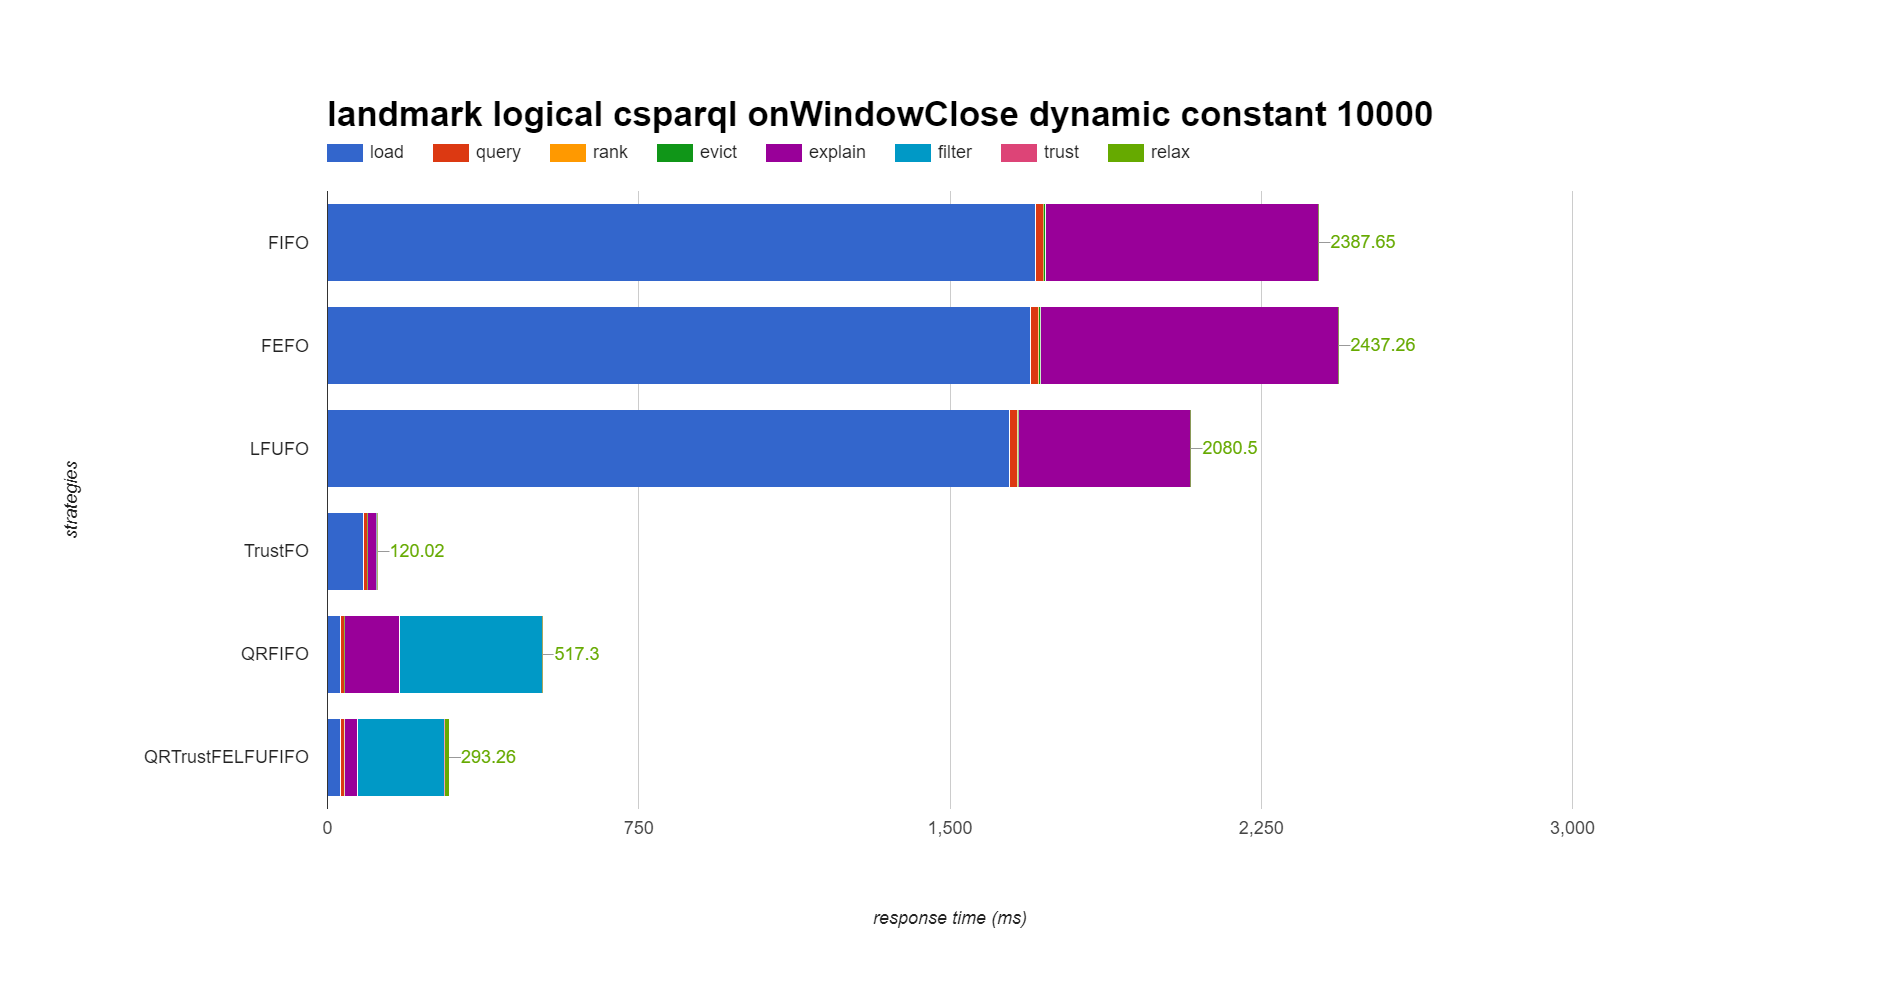
\includegraphics[width=6.5in]{img/6-1wt.png}
    \caption{\textbf{Constant Stream Mode 10k Rate Response Time}}
    \label{fig:6-csmrrt1}
\end{figure}

\begin{figure}[!htbp]
	\centering
    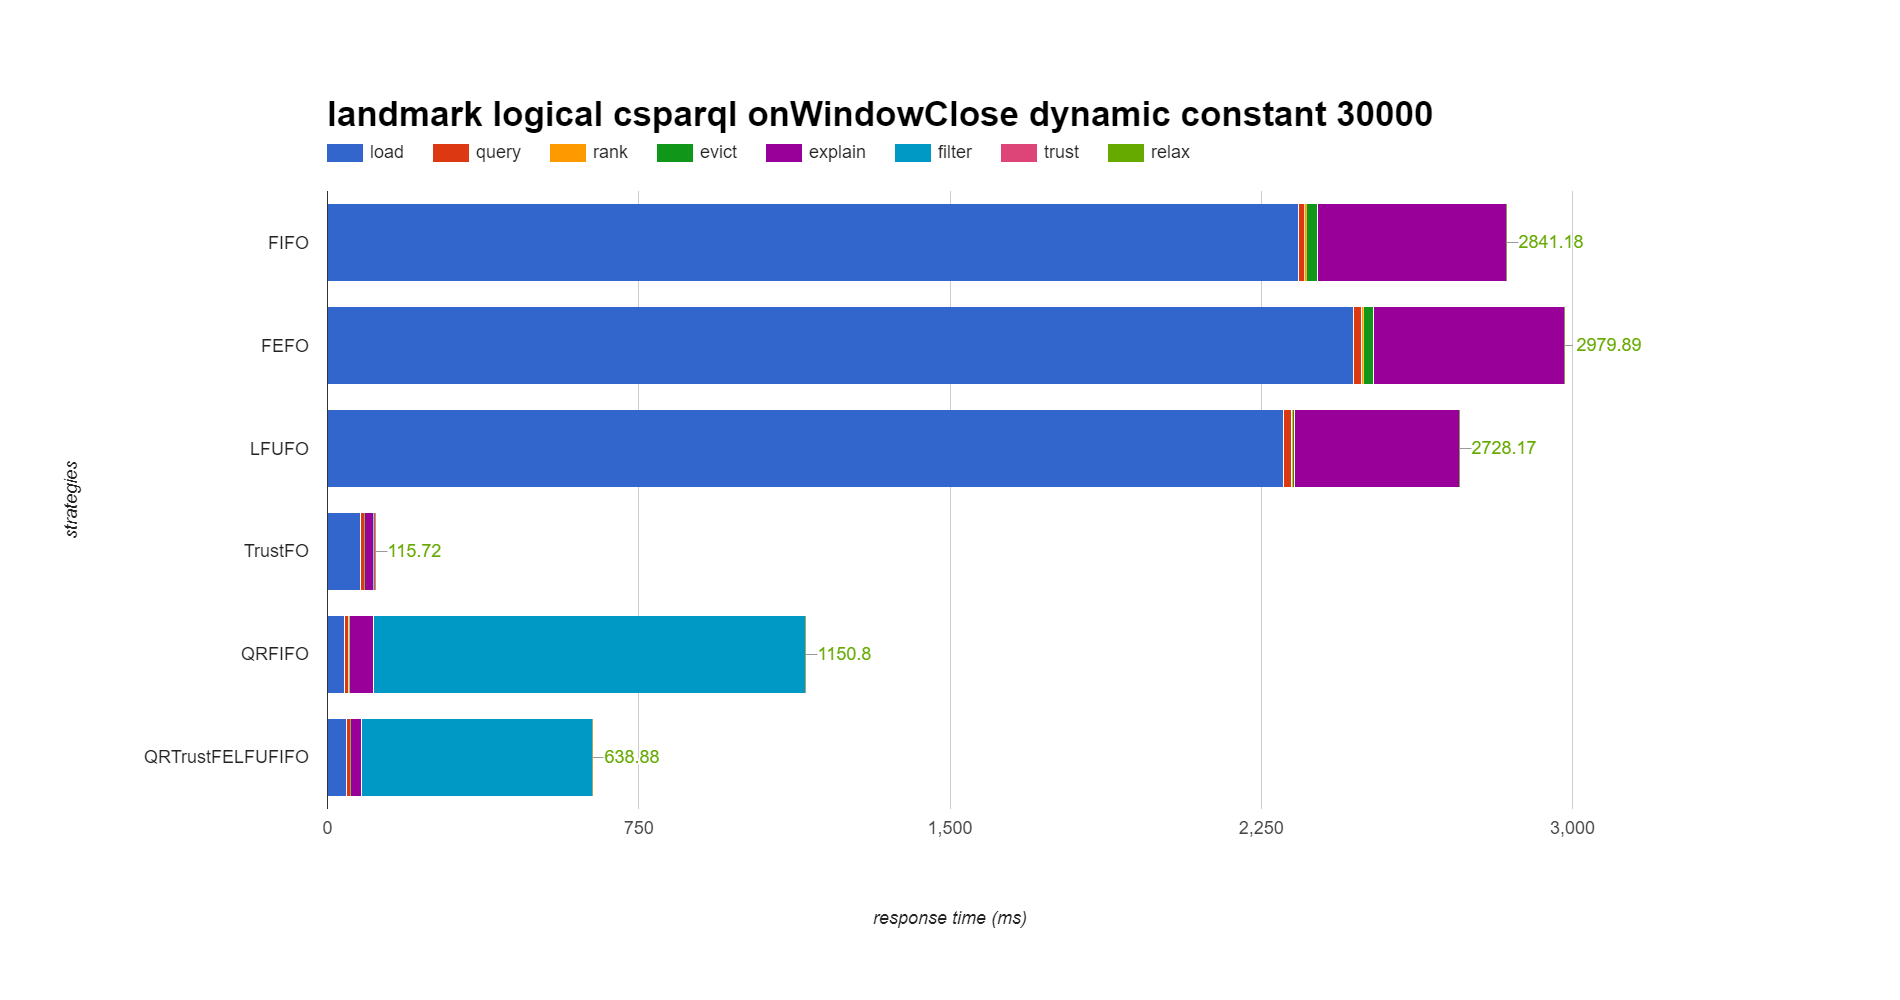
\includegraphics[width=6.5in]{img/6-3wt.png}
    \caption{\textbf{Constant Stream Mode 30k Rate Response Time}}
    \label{fig:6-csmrrt3}
\end{figure}

\begin{figure}[!htbp]
	\centering
    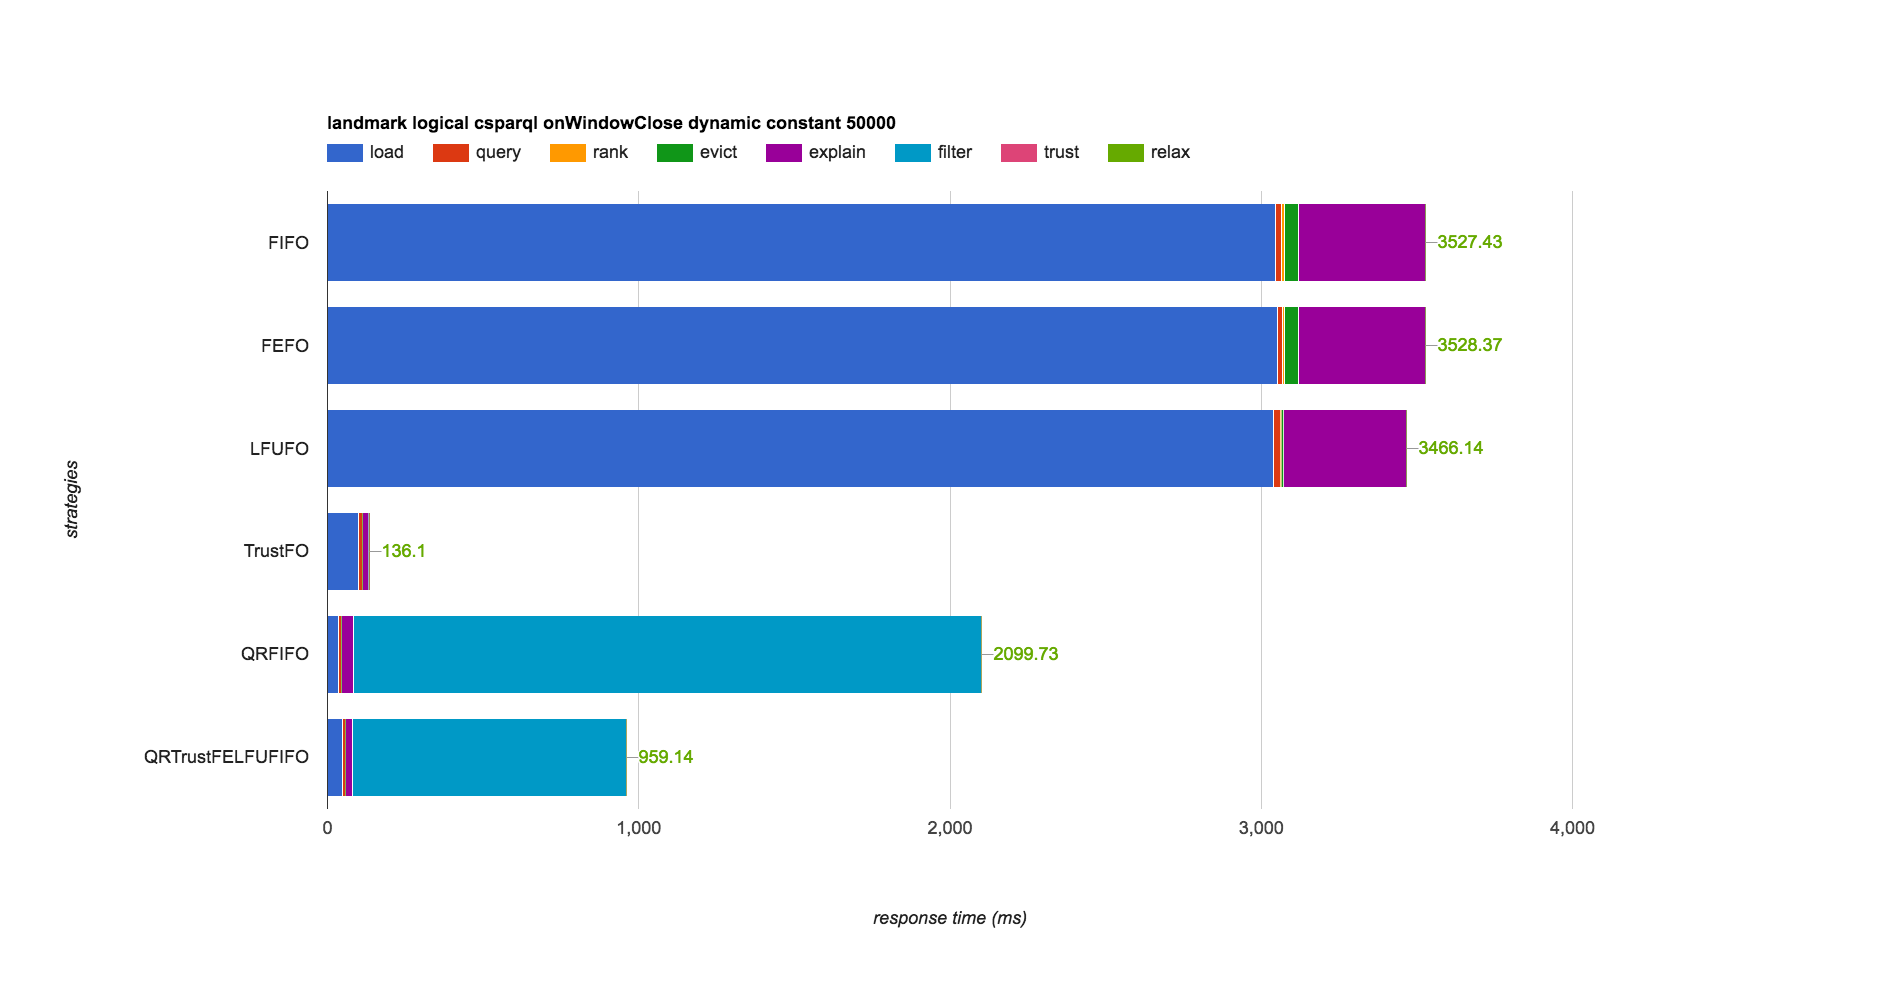
\includegraphics[width=6.5in]{img/6-5wt.png}
    \caption{\textbf{Constant Stream Mode 50k Rate Response Time}}
    \label{fig:6-csmrrt5}
\end{figure}

\begin{figure}[!htbp]
	\centering
    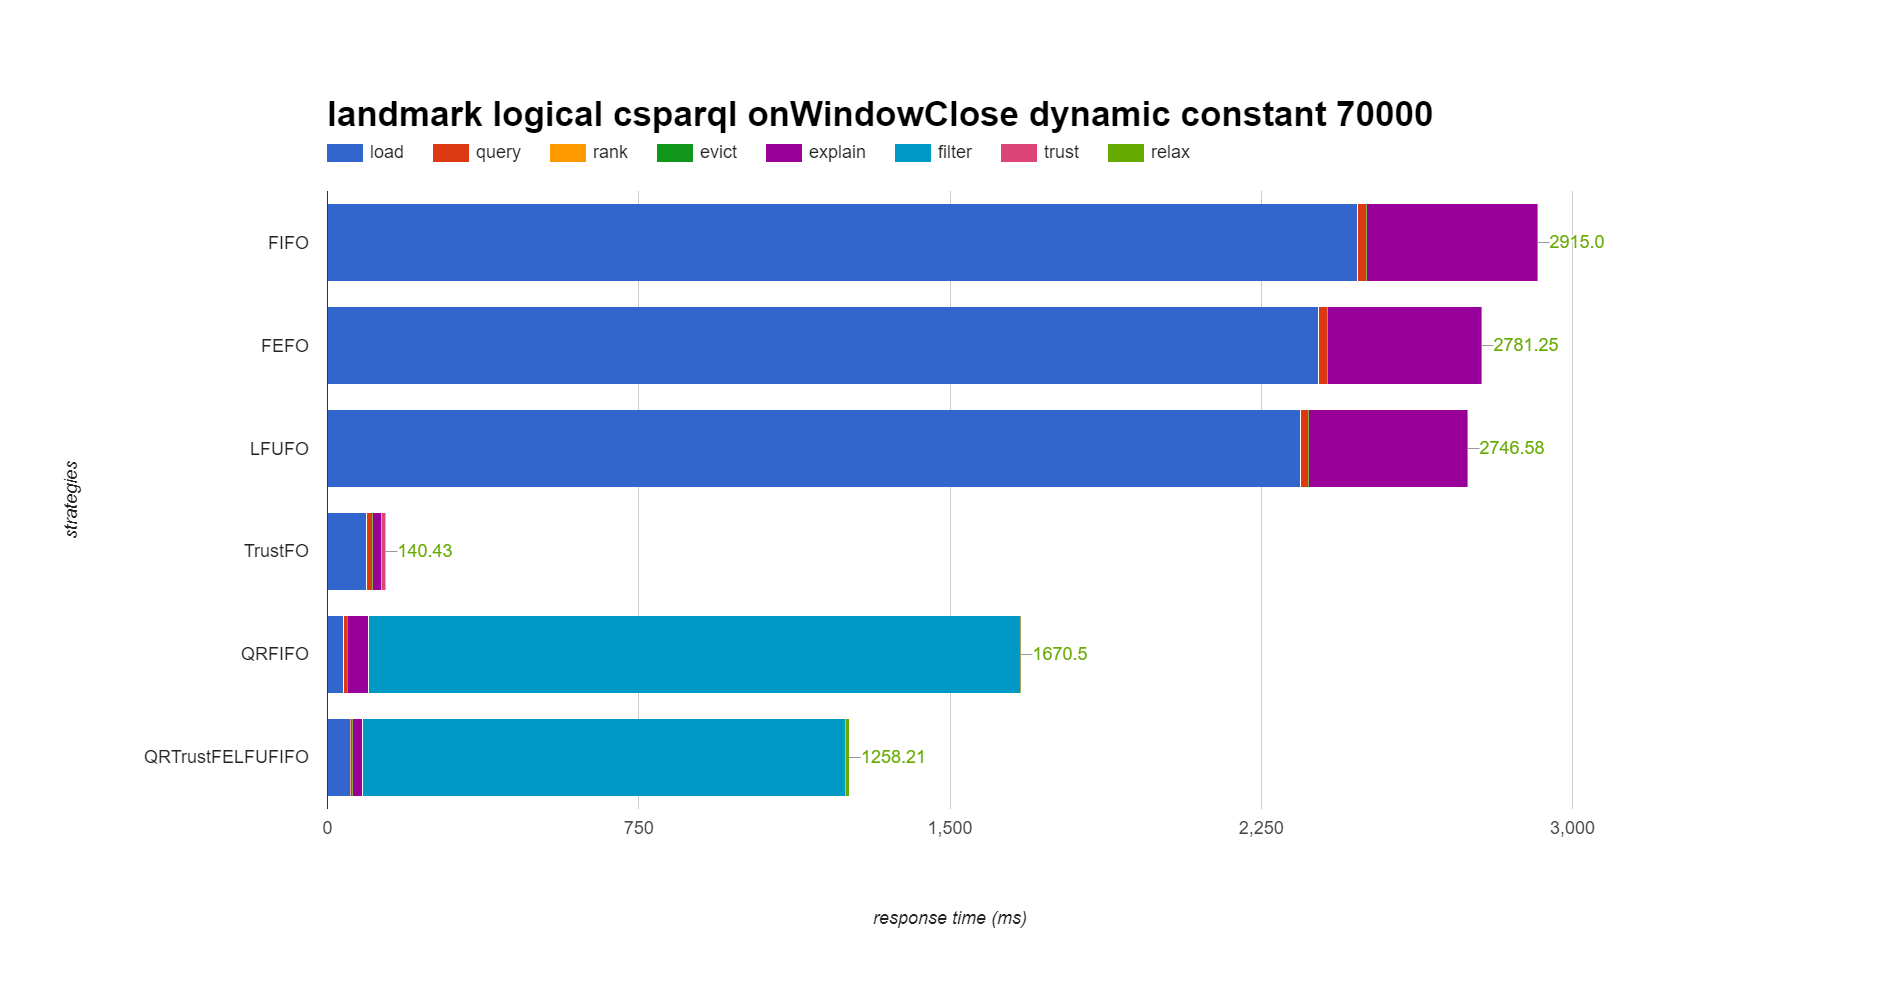
\includegraphics[width=6.5in]{img/6-7wt.png}
    \caption{\textbf{Constant Stream Mode 70k Rate Response Time}}
    \label{fig:6-csmrrt7}
\end{figure}

\begin{figure}[!htbp]
	\centering
    \includegraphics[width=6.5in]{img/6-9wt.png}
    \caption{\textbf{Constant Stream Mode 90k Rate Response Time}}
    \label{fig:6-csmrrt9}
\end{figure}

In f mode though, things become different. 
Since now the streaming rate is the peak value with 1/6 appearance probability, the average data items arrived is surely less than that in c mode. 
Thus all strategies can perform slightly better than what they do in c mode. 

\begin{figure}[!htbp]
	\centering
    \includegraphics[width=5in]{img/6-fluctuating.png}
    \caption{\textbf{FIFO Response Time Fluctuates with Stream Rate}}
    \label{fig:6-fluc}
\end{figure}

\begin{figure}[!htbp]
	\centering
    \includegraphics[width=5in]{img/6-flat.png}
    \caption{\textbf{QR-Trust-FE-LFU-FI-FO Response Time is Stable}}
   	\label{fig:6-flat}
\end{figure}

Figure \ref{fig:6-fluc} shows how FIFO's response time fluctuates with the streaming rate.
Stream reasoning system should be able to deal with stream bursts, which means that the system should not lose response when data behaves with a sudden large rate increase. 
Figure \ref{fig:6-flat} shows that semantic importance enabled window management strategy is able to keep a steady response time regardless of the streaming rate, which indicates that semantic importance is able to provide good system availability when facing versatile data streams. 
%
\subsection{Window}
Window is an important part of stream reasoning systems. 
SIGenBench is flexible in configuring different types of windows.
The results also show a significant relation between the window and the performance metrics.
This section introduces some observations and brings up some discussions. 
%
\subsubsection{Window Size}
Naively, the bigger the window size is, the more data it contains.
This means that the window can ``see'' a bigger snapshot of the data, which makes it possible to provide better performance in precision. 
However, the evaluation will show that this is not generally true, especially when the data expires quickly. 
Table \ref{tab:6-wes} shows the experiments setup.

\begin{table}[!htbp]
	\centering
    \caption{\textbf{Window Experiment Setup}}
    \label{tab:6-wes}
    \begin{tabular}{|c|l|} \hline
    \multicolumn{2}{|c|}{\textbf{experiment configuration}} \\ \hline
    window & report policy = onWindowClose \\ \hline
    data stream & \makecell[l]{lubm = 1 \\ sm = c (constant) \\ sr = 10000 data items/second \\ t = 3 (trust model 3)} \\ \hline
    query & \makecell[l]{CSPARQL target query \\ query relevance filter query 1 as in Listing 6.9} \\ \hline
    \multicolumn{2}{|c|}{\textbf{experiment variable}} \\ \hline
    window & \makecell[l]{logical sliding window \\ window size = 1s, 3s, 5s, 7s, 9s \\ window step = 1s \\ strategy: FIFO, QR-FI-FO} \\ \cline{2-2}
           & \makecell[l]{logical lower-bounded landmark window \\ initial window size = 1s, 3s, 5s, 7s, 9s worth of data items \\ window step = 1s worth of data items \\ strategy: FIFO, QR-FI-FO, FE-FO, LFU-FO, Trust-FO \\ QR-Trust-FE-LFU-FI-FO} \\ \hline
    data expiration & \makecell[l]{ets = 1 quick expiration (1s to 3s) \\ ets = 2 normal expiration (3s to 7s) \\ ets = 3 slow expiration (7s to 10s) \\ ets = 4 implicit} \\ \hline
    \end{tabular}
\end{table}

\begin{center}
	\begin{longtable}{|c||c||c|c|c|c|c|}
	\caption{\textbf{Sliding Window Size Performance}} \label{tab:6-swsp} \\
	\hline expiration & strategy & \makecell{window \\ size} & memory & \makecell{response \\ time} & precision & \makecell{through-\\put} \\ \hhline{|=#=#=|=|=|=|=|}
	\endfirsthead
	\multicolumn{7}{c} {{\bfseries \tablename\ \thetable{} -- continued from previous page}} \\
	\hline expiration & strategy & \makecell{window \\ size} & memory & \makecell{response \\ time} & precision & \makecell{through-\\put} \\ \hline 
	\endhead
	\hline \multicolumn{7}{|r|}{{Continued on next page}} \\ \hline
	\endfoot
	\hline
	\endlastfoot    
        quick & FIFO & 1s & 9999.10 & 2397.45 & 1 & 3816.67 \\ \cline{3-7}
			  &	     & 3s & 12506.25 & 2713.23 & 0 & 3969.17 \\ \cline{3-7}
			  &      & 5s & 16691.67 & 2816.50 & 0 & 4635.94 \\ \cline{3-7}
			  &      & 7s & 24997.75 & 3342.02 & 0 & 5416.76 \\ \cline{3-7}
			  &      & 9s & 49995.50 & 5517.47 & 0 & 5691.2 \\ \cline{2-7}
			  & QR-FI-FO & 1s & 13.90 & 413.81 & 1 & 31280.34 \\ \cline{3-7}
			  &		     & 3s & 27.00 & 292.25 & 1 & 37555.10 \\ \cline{3-7}
			  &          & 5s & 47.71 & 282.28 & 1 & 36745.25 \\ \cline{3-7}
			  &          & 7s & 69.80 & 305.25 & 1 & 33223.73 \\ \cline{3-7}
			  &          & 9s & 97.33 & 292.95 & 1 & 34335.72 \\ \hhline{|=#=#=|=|=|=|=|}
        normal & FIFO & 1s & 9999.10 & 2486.20 & 0.8 & 3578.65 \\ \cline{3-7}
			   &	  & 3s & 12498.88 & 2732.78 & 1 & 3826.70 \\ \cline{3-7}
			   &      & 5s & 16665.17 & 3028.36 & 0 & 4254.73 \\ \cline{3-7}
			   &      & 7s & 24997.75 & 3230.50 & 0 & 5326.08 \\ \cline{3-7}
			   &      & 9s & 49995.50 & 4990.23 & 0 & 6035.96 \\ \cline{2-7}
			   & QR-FI-FO & 1s & 14.00 & 532.62 & 1 & 24508.78 \\ \cline{3-7}
			   &		  & 3s & 29.62 & 271.65 & 1 & 39502.95 \\ \cline{3-7}
			   &          & 5s & 48.00 & 263.85 & 1 & 38786.65 \\ \cline{3-7}
			   &          & 7s & 75.00 & 281.03 & 1 & 35005.22 \\ \cline{3-7}
			   &          & 9s & 97.67 & 294.49 & 1 & 34277.19 \\ \hhline{|=#=#=|=|=|=|=|}
        slow  & FIFO & 1s & 9999.1 & 2489.96 & 1 & 3820.44 \\ \cline{3-7}
			  &	     & 3s & 12498.88 & 2716.76 & 1& 3939.00 \\ \cline{3-7}
			  &      & 5s & 16665.17 & 2994.14 & 1& 4356.12 \\ \cline{3-7}
			  &      & 7s & 24997.75 & 3283.32 & 1& 5392.64 \\ \cline{3-7}
			  &      & 9s & 49995.50 & 4906.29 & 1& 6294.06 \\ \cline{2-7}
			  & QR-FI-FO & 1s & 13.80 & 476.61 & 1 & 24921.91 \\ \cline{3-7}
			  &		     & 3s & 28.50 & 272,70 & 1 & 39057.89 \\ \cline{3-7}
			  &          & 5s & 47.14 & 273.08 & 1 & 36624.77 \\ \cline{3-7}
			  &          & 7s & 70.20 & 269.89 & 1 & 36785.58 \\ \cline{3-7}
			  &          & 9s & 96.67 & 284.10 & 1 & 36531.61 \\ \hhline{|=#=#=|=|=|=|=|}
        none   & FIFO & 1s & 9999.10 & 2307.75 & 1 & 3919.80 \\ \cline{3-7}
			   &	  & 3s & 12498.88 & 2587.18 & 1 & 4106.65 \\ \cline{3-7}
			   &      & 5s & 16665.17 & 2928.87 & 1 & 4496.00 \\ \cline{3-7}
			   &      & 7s & 19998.20 & 2876.45 & 1 & 5260.03 \\ \cline{3-7}
			   &      & 9s & 49995.50 & 4704.67 & 1 & 6653.98 \\ \cline{2-7}
			   & QR-FI-FO & 1s & 13.90 & 683.52 & 1 & 18572.88\\ \cline{3-7}
			   &		  & 3s & 28.25 & 276.81 & 1 & 39690.09\\ \cline{3-7}
			   &          & 5s & 49.57 & 274.90 & 1 & 39302.19\\ \cline{3-7}
			   &          & 7s & 72.80 & 281.03 & 1 & 37639.46\\ \cline{3-7}
			   &          & 9s & 97.00 & 283.03 & 1 & 36268.04 \\              
\end{longtable}
    \begin{tablenotes}
 		\item memory unit: number of data items
 		\item response time unit: ms
 		\item throughput unit: data items/second
    \end{tablenotes}
\end{center}

\begin{center}
	\begin{longtable}{|c||c||c|c|c|c|c|}
	\caption{\textbf{Landmark Window Size Performance}} \label{tab:6-lwsp} \\
	\hline expiration & strategy & \makecell{window \\ size} & memory & \makecell{response \\ time} & precision & \makecell{through-\\put} \\ \hhline{|=#=#=|=|=|=|=|}
	\endfirsthead
	\multicolumn{7}{c} {{\bfseries \tablename\ \thetable{} -- continued from previous page}} \\
	\hline expiration & strategy & \makecell{window \\ size} & memory & \makecell{response \\ time} & precision & \makecell{through-\\put} \\ \hline 
	\endhead
	\hline \multicolumn{7}{|r|}{{Continued on next page}} \\ \hline
	\endfoot
	\hline
	\endlastfoot    
        quick & FIFO & 1s & 9999.10 & 2430.96 & 0.50 & 3752.29 \\ \cline{3-7}
			  &	     & 3s & 12498.88 & 2774.65 & 0 & 3795.21 \\ \cline{3-7}
			  &      & 5s & 16665.17 & 2818.66 & 0 & 4588.54 \\ \cline{3-7}
			  &      & 7s & 24997.75 & 3359.35 & 0 & 5153.53 \\ \cline{3-7}
			  &      & 9s & 49995.50 & 4847.37 & 0 & 6298.00 \\ \cline{2-7}
			  & QR-FI-FO & 1s & 14.00 & 284.13 & 1& 38445.51\\ \cline{3-7}
			  &		     & 3s & 28.50 & 281.85 & 1& 37866.29\\ \cline{3-7}
			  &          & 5s & 51.67 & 281.55 & 1& 37681.78\\ \cline{3-7}
			  &          & 7s & 75.00 & 308.26 & 1& 33850.17\\ \cline{3-7}
			  &          & 9s & 101.33 & 305.02 & 1& 36505.08\\ \cline{2-7}
			  & FE-FO & 1s & 10756.00 & 2531.39 & 0.50 & 3541.09 \\ \cline{3-7}
			  &		  & 3s & 12498.88 & 2691.70 & 1 & 3931.45 \\ \cline{3-7}
			  &       & 5s & 16665.17 & 2897.93 & 0 & 4484.57 \\ \cline{3-7}
			  &       & 7s & 24997.75 & 3336.05 & 0 & 5185.42 \\ \cline{3-7}
			  &       & 9s & 49995.50 & 4747.63 & 0 & 6456.97 \\ \cline{2-7}
			  & LFU-FO & 1s & 10045.40 & 2132.99 & 0.50 & 1938.02 \\ \cline{3-7}
			  &		   & 3s & 12541.50 & 2279.74 & 0 & 2072.37 \\ \cline{3-7}
			  &        & 5s & 16717.17 & 2578.32 & 0 & 2390.56 \\ \cline{3-7}
			  &        & 7s & 25054.50 & 3175.83 & 0 & 3084.56 \\ \cline{3-7}
			  &        & 9s & 50044.50 & 4664.32 & 0 & 4838.07 \\ \cline{2-7}
			  & Trust-FO & 1s & 633.70 & 103.04 & 1 & 50698.44\\ \cline{3-7}
			  &			 & 3s & 3663.12 & 188.17 & 1& 41681.18\\ \cline{3-7}
			  &          & 5s & 1727.67 & 148.26 & 1& 57547.22\\ \cline{3-7}
			  &          & 7s & 2911.50 & 170.09 & 1& 75533.43\\ \cline{3-7}
			  &          & 9s & 4298.00 & 205.83 & 1& 115557.47\\ \cline{2-7}
              & QR-Trust- & 1s & 23.80 & 280.54 & 1& 36373.01\\ \cline{3-7}
			  &	FE-LFU-   & 3s & 27.38 & 280.88 & 1& 38139.23\\ \cline{3-7}
			  & FI-FO     & 5s & 30.29 & 283.78 & 1& 38226.24\\ \cline{3-7}
			  &           & 7s & 41.40 & 298.30 & 1& 37966.39\\ \cline{3-7}
			  &           & 9s & 53.00 & 289.23 & 1& 41373.43\\ \hhline{|=#=#=|=|=|=|=|}
        normal & FIFO & 1s & 9999.10 & 2419.96 & 0.80 & 3667.82 \\ \cline{3-7}
			   &	  & 3s & 12498.88 & 2674.31 & 0.67 & 3837.80 \\ \cline{3-7}
			   &      & 5s & 16683.33 & 3000.33 & 0 & 4305.57 \\ \cline{3-7}
			   &      & 7s & 24997.75 & 3265.81 & 0 & 5274.38 \\ \cline{3-7}
			   &      & 9s & 49995.50 & 4582.60 & 0 & 6670.76 \\ \cline{2-7}
			   & QR-FI-FO & 1s & 14.00 & 266.50 & 1 & 40456.74 \\ \cline{3-7}
			   &		  & 3s & 29.75 & 274.62 & 1 & 39103.46\\ \cline{3-7}
			   &          & 5s & 48.14 & 271.19 & 1 & 37909.13 \\ \cline{3-7}
			   &          & 7s & 76.20 & 279.30 & 1 & 35815.82 \\ \cline{3-7}
			   &          & 9s & 97.00 & 279.83 & 1 & 37002.21 \\ \cline{2-7}
			   & FE-FO & 1s & 13623.80 & 2463.58 & 1 & 3373.77 \\ \cline{3-7}
			   &	   & 3s & 15852.12 & 2736.27 & 1 & 3667.55 \\ \cline{3-7}
			   &       & 5s & 18404.50 & 3085.17 & 0 & 4192.63 \\ \cline{3-7}
			   &       & 7s & 24997.75 & 3264.10 & 0 & 5285.47 \\ \cline{3-7}
			   &       & 9s & 49995.50 & 4749.43 & 1 & 6437.54 \\ \cline{2-7}
			   & LFU-FO & 1s & 10048.00 & 2057.90 & 1 & 2093.87 \\ \cline{3-7}
			   &		& 3s & 12533.12 & 2313.39 & 1 & 2214.87 \\ \cline{3-7}
			   &        & 5s & 16707.50 & 2599.38 & 0 & 2497.70 \\ \cline{3-7}
			   &        & 7s & 25046.25 & 3091.38 & 0 & 3180.38 \\ \cline{3-7}
			   &        & 9s & 50035.50 & 4554.67 & 0 & 4853.48 \\ \cline{2-7}
			   & Trust-FO & 1s & 621.10 & 105.11 & 1 & 51929.24\\ \cline{3-7}
			   &		  & 3s & 3632.88 & 179.74 & 1& 43540.49\\ \cline{3-7}
			   &          & 5s & 1720.17 & 140.26 & 1& 60236.67\\ \cline{3-7}
			   &          & 7s & 2927.25 & 179.86 & 1& 72851.45\\ \cline{3-7}
			   &          & 9s & 4350.50 & 207.43 & 1& 119400.24\\ \cline{2-7}
               & QR-Trust- & 1s & 49.20 & 276.39 & 1 & 34300.58\\ \cline{3-7}
			   & FE-LFU-   & 3s & 56.62 & 267.66 & 1 & 35337.43\\ \cline{3-7}
			   & FI-FO     & 5s & 58.86 & 277.59 & 1 & 35474.59\\ \cline{3-7}
			   &           & 7s & 63.80 & 289.14 & 1 & 35905.36\\ \cline{3-7}
			   &           & 9s & 73.33 & 280.02 & 1 & 39179.66\\ \hhline{|=#=#=|=|=|=|=|}
        slow  & FIFO & 1s & 9999.10 & 2495.20 & 1 & 3815.66 \\ \cline{3-7}
			  &	     & 3s & 12498.88 & 2758.74 & 1 & 3789.91 \\ \cline{3-7}
			  &      & 5s & 16665.17 & 3033.92 & 1 & 4334.53 \\ \cline{3-7}
			  &      & 7s & 24997.75 & 3298.89 & 1 & 5377.64 \\ \cline{3-7}
			  &      & 9s & 49995.50 & 4734.86 & 1 & 6611.63 \\ \cline{2-7}
			  & QR-FI-FO & 1s & 13.80 & 263.60 & 1 & 41068.22 \\ \cline{3-7}
			  &		     & 3s & 27.38 & 257.78 & 1 & 41135.43 \\ \cline{3-7}
			  &          & 5s & 46.71 & 266.54 & 1 & 37471.11 \\ \cline{3-7}
			  &          & 7s & 73.00 & 273.52 & 1 & 36718.41 \\ \cline{3-7}
			  &          & 9s & 96.67 & 265.43 & 1 & 39118.68 \\ \cline{2-7}
			  & FE-FO & 1s & 17786.00 & 2614.28 & 1 & 3063.04 \\ \cline{3-7}
			  &		  & 3s & 20244.25 & 2907.29 & 1 & 3336.60 \\ \cline{3-7}
			  &       & 5s & 24809.00 & 3263.75 & 1 & 3616.50 \\ \cline{3-7}
			  &       & 7s & 29148.25 & 3436.78 & 1 & 5034.55 \\ \cline{3-7}
			  &       & 9s & 51284.00 & 4785.86 & 1 & 6618.06 \\ \cline{2-7}
			  & LFU-FO & 1s & 12256.30 & 2180.53 & 1 & 2118.27\\ \cline{3-7}
			  &		   & 3s & 12529.62 & 2297.83 & 1 & 2279.03 \\ \cline{3-7}
			  &        & 5s & 16701.83 & 2592.45 & 1 & 2591.91 \\ \cline{3-7}
			  &        & 7s & 25035.25 & 3127.57 & 1 & 3288.47 \\ \cline{3-7}
			  &        & 9s & 50024.00 & 4648.54 & 1 & 5091.41 \\ \cline{2-7}
			  & Trust-FO & 1s & 644.70 & 109.56 & 1 & 52009.83 \\ \cline{3-7}
			  &			    & 3s & 3726.50 & 195.68 & 1& 42545.49\\ \cline{3-7}
			  &             & 5s & 1740.17 & 148.78 & 1& 59877.90\\ \cline{3-7}
			  &             & 7s & 2938.00 & 184.45 & 1& 73760.09\\ \cline{3-7}
			  &          & 9s & 4344.50 & 205.12 & 1& 118976.33\\ \cline{2-7}
              & QR-Trust- & 1s & 64.00 & 268.07 & 1& 31875.40 \\ \cline{3-7}
			  &	FE-LFU-   & 3s & 75.62 & 260.77 & 1& 32973.11 \\ \cline{3-7}
			  & FI-FO     & 5s & 80.14 & 274.95 & 1& 32462.06 \\ \cline{3-7}
			  &           & 7s & 89.80 & 276.26 & 1& 33907.25 \\ \cline{3-7}
			  &           & 9s & 99.33 & 268.83 & 1& 38386.79 \\ \hhline{|=#=#=|=|=|=|=|}
        none   & FIFO & 1s & 9999.10 & 2294.27 & 1 & 3948.59 \\ \cline{3-7}
			   &	  & 3s & 12498.88 & 2602.75 & 1 & 3994.08 \\ \cline{3-7}
			   &      & 5s & 16665.17 & 3020.46 & 1 & 4367.48 \\ \cline{3-7}
			   &      & 7s & 24997.75 & 3235.59 & 1 & 5495.22 \\ \cline{3-7}
			   &      & 9s & 49995.50 & 4540.93 & 1 & 7001.04 \\ \cline{2-7}
			   & QR-FI-FO & 1s & 13.90 & 252.62 & 1 & 43018.83 \\ \cline{3-7}
			   &		  & 3s & 28.62 & 270.16 & 1 & 40294.59 \\ \cline{3-7}
			   &          & 5s & 49.57 & 279.72 & 1 & 38342.87 \\ \cline{3-7}
			   &          & 7s & 73.00 & 267.42 & 1 & 39088.26 \\ \cline{3-7}
			   &          & 9s & 97.00 & 271.25 & 1 & 39286.83 \\ \cline{2-7}
 			   & FE-FO\footnote{FE-FO can not run because of no data expiration.} & 1s & - & - & - & - \\ \cline{3-7}
			   &	   & 3s & - & - & - & - \\ \cline{3-7}
			   &       & 5s & - & - & - & - \\ \cline{3-7}
			   &       & 7s & - & - & - & - \\ \cline{3-7}
			   &       & 9s & - & - & - & - \\ \cline{2-7}
			   & LFU-FO & 1s & 10043.10 & 2088.77 & 1 & 1963.50 \\ \cline{3-7}
			   &		& 3s & 12533.25 & 2266.74 & 1 & 2091.60 \\ \cline{3-7}
			   &        & 5s & 16706.17 & 2557.57 & 1 & 2395.06 \\ \cline{3-7}
			   &        & 7s & 24043.50 & 3052.05 & 1 & 3083.90 \\ \cline{3-7}
			   &        & 9s & 50031.50 & 4666.90 & 1 & 4700.31 \\ \cline{2-7}
			   & Trust-FO & 1s & 638.20 & 108.65 & 1& 52334.72 \\ \cline{3-7}
			   &			 & 3s & 3705.00 & 199.62 & 1& 42599.58 \\ \cline{3-7}
			   &             & 5s & 1727.83 & 147.46 & 1& 61004.25 \\ \cline{3-7}
			   &             & 7s & 2929.50 & 164.79 & 1& 77156.56 \\ \cline{3-7}
			   &          & 9s & 4337.00 & 222.00 & 1& 111829.81 \\ \cline{2-7}
              & QR-Trust- & 1s & 34.70 & 264.92 & 1 & 30697.71 \\ \cline{3-7}
			  &	FE-LFU-   & 3s & 39.25 & 258.48 & 1 & 31684.53 \\ \cline{3-7}
			  & FI-FO     & 5s & 45.83 & 262.53 & 1 & 32078.81 \\ \cline{3-7}
			  &           & 7s & 42.60 & 271.61 & 1 & 32704.94 \\ \cline{3-7}
			  &           & 9s & 61.00 & 266.88 & 1 & 36624.77 \\
\end{longtable}
    \begin{tablenotes}
 		\item memory unit: number of data items
 		\item response time unit: ms
 		\item throughput unit: data items/second
    \end{tablenotes}
\end{center}

Table \ref{tab:6-swsp} shows sliding window size performance. 
Only two strategies FIFO and QR-FI-FO are employed so as to maintain the integrity of the sliding window semantics. 

FIFO tends to consume much more memory than QR-FI-FO in all scenarios. 
Both strategies consume more memory as the window size increases. 
QR-FI-FO manages to keep the response time within 1 second, while FIFO's response time increases as the window size increases. 
When data expires quickly, FIFO's precision drops as window size increases.
As data expires slowly, FIFO is able to keep a good precision. 
QR-FI-FO's precision is always 1, regardless how data expires or window size is. 
FIFO's throughput is way less than that of QR-FI-FO, in fact FIFO's throughput is less than the streaming rate.

Table \ref{tab:6-lwsp} shows the performance of landmark window size. 
Lower-bounded landmark window will only have its upper bound proceeds. 
According to the extended window semantics, the window definition sets the initial window size of a lower-bounded window size. 
FIFO and QR-FI-FO's performance is quite similar as in Table \ref{tab:6-swsp}. 
It can also be seen that FE-FO and LFU-FO performs similar as FIFO. 
Strategies with QR or trust aspect is capable to perform well even if window size increases. 
The compound strategy QR-Trust-FE-LFU-FI-FO shows a good performance as well. 

The results show a strong correlation among the four metrics: the strategy will perform better as long as the memory consumption is small.
With a small amount of data items in the window, response time will be fast, thus the system is able to keep up with the streaming data rate and expiration, thus the precision and throughput are improved. 
Data expiration also plays an important role for strategy performance. 
Strategies that can manage data in a fast speed can keep up with fast data expiration, which is the main reason to achieve the precision of 1. 
As the data expires slowly, all strategies can deliver good precision, because the data expiration is more tolerant with longer system processing time.
%
\subsubsection{Report Policy}
Report policies are part of window semantics. 
They determine the condition to fire the query and report the results.
They are also part of the reasons to explain the different results reported by different stream reasoning engines \cite{dell2013correctness}.
SIGenBench supports four report policies.
However, the influences of them on stream reasoning systems have already been discussed in the related work \cite{dell2013correctness}.
%
\subsubsection{Strategy}
Different window management strategies are supported by different combinations of semantic importance aspects, which views data importance in different ways, thus can provide different results and performances. 
However, the performance of any strategy is not only dependent on its semantic importance aspects, but also the environment it is deployed. 
For example, if the streaming data carries its own trust score, it is generally a good idea to add the trustworthiness in the strategy. 
In all ways, query relevance filtering is recommended because of its huge positive influence to the system performance.
The reason to enable so many possible strategies from semantic importance is to allow the flexibility of choosing an appropriate one that can work well in a specific use case. 
This requires the users to be aware of the traits in their own use cases, as well as the performance impacts by different semantic importance aspect.
The above experiments have already shown all the strategies' performances under different scenarios.
%
\section{Summary}
The above experiments have illustrated that SIGenBench is both powerful and flexible to generalize and benchmark semantic importance. 
Query relevance can significantly increase the strategy performance as in Table \ref{tab:6-qrp}.
From the experimental results it can also be seen that different filtering queries can definitely affect system performance. 
For example, Query 1 can comprehensively improve stream reasoning systems.
Even Query 2 or 3 query relevance can still improve system response time. 
However, it can also be seen that as streaming rate increases, query relevance can reach the limitation where filtering time can take too long, which can negatively impact the response time and precision. 
Temporal provenance, especially the expiration timestamp, is suitable where data carries explicit expiration timestamps. 
They are good at picking up expired data to avoid invalid query results. 
However, in order to guarantee system response time, the experimental results recommend to work with QR aspect. 
Query participation, although does not show an outstanding performance improvement, is still an important aspect. 
It is able to keep the partial necessary data items and wait for the other necessary data items to answer the query, which can improve system precision. 
From the experimental results, it is recommended to work with QR to improve system metrics, as well as temporal provenance if explicit expiration timestamps are carried. 
Trustworthiness is very straightforward. 
It relies trust models to assign numerical trust scores, based on which the data can be ranked. 
The experimental results have shown that different trust models can yield different system results. 
The algorithm to rank trust scores only takes O(n), where n is the number of data items in the window. 
This means trust aspect can run much faster, thus it is recommended to consider trustworthiness when data carries trust scores. 
Finally, a compound strategy like QR-Trust-FE-LFU-FI-FO considers multiple importance factors, and achieves far better performance than FIFO. 
This finding has already proves that semantic importance enabled window management strategies are able to improve the stream reasoning systems. 
%%%%%%%%%%%%%%%%%%%%%%%%%%%%%%%%%%%%%%%%%%%%%%%%%%%%%%%%%%%%%%%%%%%% 
%                                                                 %
%                            CHAPTER SEVEN                        %
%                                                                 %
%%%%%%%%%%%%%%%%%%%%%%%%%%%%%%%%%%%%%%%%%%%%%%%%%%%%%%%%%%%%%%%%%%% 
 
\chapter{CONCLUSION AND FUTURE WORK}
Semantic importance (SI) is a powerful and flexible way to model the importance of streaming data from various data orderings.
The evaluation results have shown that SI is powerful at reducing system overhead and increasing system performance. 
The flexibility lies in the fact that SI supports a range of window management strategies that can efficiently manage the data in the window. 
SI is also expendable thanks to the SI ontology, which also helps understand what SI is really about by providing grounded instances.
Implemented in OWL, SI ontology can be easily edited in ontology composing tools so that new aspects can be added. 
This chapter concludes this dissertation, and provide future insights on where SI can go from current standing point. 
%
\section{Conclusion}
The core contribution of this dissertation is to propose the notion of semantic importance, along with a set of infrastructure to enable the usage of semantic importance in the stream reasoning settings.
Exemplar use case implementations have shown show how semantic importance can be leveraged in real-world scenarios.
The comprehensive generalization and benchmark framework connects semantic importance to the state-of-the-art stream reasoning techniques, which allows testing system performances with multiple dimensional configuration parameters.

The motivation to propose semantic importance originally comes from the situations where the temporal silent assumption can fail.
The temporal silent assumption, which regards the most recent data as the most important, only concentrates on one explicit data ordering -- arrival order. 
This will cause two problems, namely early eviction and early expiration, as it has been shown in Chapter 1.
It has been observed that these two problems are caused because the system is not able to distinguish the data based on its priority. 
Such priority, often implicit, leads to the efforts to make it visible for the processing system, which is formalized in the concept of semantic importance.
Semantic importance is derived from various data orderings, and currently provide four general aspects that can support a wide range of window management strategies.
Like FIFO, these strategies help window to identify more important data with one or multiple data orderings; but unlike FIFO, these strategies provide more flexible options to choose under different stream reasoning scenarios, which can improve system performance.
Chapter 2 shows what semantic importance is, as well as its incompatibility of the existing window semantics that only works with FIFO.
In order to deploy semantic importance in stream reasoning systems without breaking the integrity of window semantics, the landmark window is leveraged.
The semantics of landmark window provide a firm theoretical foundation for the application of semantic importance. 
The first set of infrastructure is the sequential stream reasoning architecture (SSRA), with the purpose of providing a first architecture to deploy semantic importance for stream reasoning use cases. 
SSRA features four components that are executed sequentially. 
Its window is implemented based on the high performance off-the-shelf triple-stores. 
SSRA shows how semantic importance can be deployed in a stream reasoning application, with experimental evidence that shows SI efficacy. 
Chapter 5 shows two use cases implementations based on different window management strategies.
They are real-world use cases with different requirements.
The results have shown that semantic importance is adaptable in different cases, and provide satisfactory system performance. 
Chapter 6 generalizes semantic importance by connecting it to the state-of-the-art stream reasoning techniques, as well as provide a software that can benchmark the performance of stream reasoning applications.
SIGenBench systematically benchmarked three categories and how each of them can affect the system performance, as well as how semantic importance can help to minimize the adverse impact and maximize the benefits. 

Stream reasoning not only requires real-time stream processing, but also on-line reasoning.
Most state-of-the-art work in stream reasoning performs logical reasoning, i.e., to provide a background ontology that contains the knowledge about the domain in the window.
A reasoner also resides in the window, which can be used to infer hidden information together with the ontology and the streaming data. 
However, logical reasoning is relatively slow, and does not scale well with large volume of data. 
One method to minimize this problem is to reduce the data items in the window. 
This can be done by either shrinking the window size or filtering the data. 
When shrinking the window size, data items get more easily to exit the window under the silent assumption, but when filtering data, the system has to make sure to filter data correctly so that all the necessary data items are kept. 
Both require the system to be data discriminative, which is enabled by semantic importance. 

Semantic importance currently includes four aspects, provenance, query participation, trustworthiness, and query relevance. 
It is designed to be flexible and extendable. 
It also comes along with an ontology that is grounded by real-life use case and instances.
Semantic importance is embodied in a priority vector, which features a preference function that the most preferred element is placed leftist, as well as a comparison rule that enables ranking.

The semantics of sliding window, which works well with the temporal silent assumption, can not be adopted when using semantic importance. 
This is because, other than FIFO, the strategies enabled by semantic importance will evict the data out of its arrival order.
This can break the semantics of the sliding window.
Thus, the landmark window is proposed to use, as its semantics works well under the semantic importance framework. 
Both time-based and tuple-based window semantics have been refined, which is not only compatible with the sliding window, but also opens up more window options to use in stream reasoning. 

Since most state-of-the-art stream reasoning work is dependant on solely sliding window, which encapsulate the window and window strategies with their internal core, it is not feasible to implement semantic importance on the top of them. 
However, their architecture and design can be referenced. 
Sequential Stream Reasoning Architecture is thus proposed. 
The core design is to let the window stand out of the processing architecture, so that it can be configured according to the users' need. 
SSRA features five main component, other than the window implemented in off-the-shelf triple-stores, the data consumption component consumes the data by sending it into the window. 
Depending on different window report policies, the query execution component is fired and thus query results are generated. 
The reasoner inside of the triple-store can provide the ability to trace back to what happened during the reasoning and query process, such that the data items participated in the query can be tracked.
At last, the data is evicted based on its semantic importance ranking.
Usually, the lower-ranked data will be evicted first. 

Based on SSRA, two use cases have been implemented. 
Both of them are within the streaming context, where the data is either streamed in high frequency or large volume. 
% something to say

Finally, SIGenBench provides the generalization and benchmark system for semantic importance. 
Semantic importance is connected to the state-of-the-art stream reasoning in SIGenBench. 
SIGenBench is carefully implemented to decouple the window semantics out of its processing engine, such as CSPARQL and CQELS. 
Currently, SIGenBench supports four kinds of window, four kinds of window report operational semantics, two kinds of continuous query language, and twenty-four different window management strategies. 
All of this opens up a great possibility to configure a window in many different ways. 
SIGenBench can also control stream rates and modes, so as to provide more simulation capabilities. 
%
\section{Future Work}
Semantic importance currently only has four aspects, among which the provenance and trustworthiness aspects are both very broad. 
This dissertation only talks about some temporal provenance, and leaves other types of provenance untouched. 
This is the first part of the future work beyond this dissertation. 
Trustworthiness is another big topic, there are trust models encoded in either math equations or ontologies.
Trustworthiness is also dependent on the domain and context. 
So this is a broad domain, but the results from this domain can be leveraged as the aspect of semantic importance, encoded in the window management strategies to bring the data-awareness of the specific application in stream reasoning.
Also we say that semantic importance is an extendable conceptual model, which encourages people to add more contents or refine this concept in order to use them in different scenarios. 
Another future work is to extend various aspects or sub-aspects to enrich the semantic importance family. 
I also plan to advocate semantic importance, so that more and more people will get to know it and try to use it. 
As long as semantic importance is being extended, the value of it will grow. 

SIGenBench is really a tool to help people reuse semantic importance.
It is generally usable, all it needs is to configure the parameter via the command line. 
Users can feed their data, ontology, and choose their desired window and stream configurations, and then run. 
The benchmark results will be given.
One restriction in this tool is that, all the strategies are currently built-in, which doesn't enable the user to choose their own desired strategies that are not listed in these strategies. 
The reason for this is that SIGenBench is implemented in Java, which is a static type language, and does not support creating classes during the run-time. 
The only way to make it work is to encode everything as a class, so that it can be called in run-time. 
So the future work is about this short-coming is two-fold.
First, to implement SIGenBench in a dynamic typed language, so that the strategies can be created during the run-time.
Second, the strategies will be supported by loading the semantic importance ontology, where the users extend, specify and edit their extended aspects.
SIGenBench should be able to create a list of possible strategies on the top of reading semantic importance ontology and let the user to specify what strategy they would like to test in their use cases. 

The third future work, is a far future one. 
As the users and use cases are being developed, the semantic importance is being extended. 
Users will choose their desired strategy. 
As this kind of data becomes more and more available, a recommendation system can be built. 
By leveraging the use case requirements, the strategies used, and supervised machine learning algorithms, a recommendation system should be able to provide some recommendations to new users, given the input of their use case requirements. 
The recommended results will be at least as a starting point from which the users will need to test their use case. 

(develop a tool that can use sio to at least compose a set of strategies)
%%%%%%%%%%%%%%%%%%%%%%%%%%%%%%%%%%%%%%%%%%%%%%%%%%%%%%%%%%%%%%%%%%%
%                                                                 %
%                           BIBLIOGRAPHY                          %
%                                                                 %
%%%%%%%%%%%%%%%%%%%%%%%%%%%%%%%%%%%%%%%%%%%%%%%%%%%%%%%%%%%%%%%%%%%

%This method produces a numbered bibliography where the numbers
%correspond to the \cite commands in the text. See the LaTeX manual.
%
\specialhead{REFERENCES}
\begin{singlespace}
\bibliographystyle{bibs/IEEEtran} % sorted by citation order
%\bibliographystyle{bibs/IEEEtranS} % sorted by first author
\bibliography{bibs/IEEEabrv,bibs/simulation}
\end{singlespace}

%%%%%%%%%%%%%%%%%%%%%%%%%%%%%%%%%%%%%%%%%%%%%%%%%%%%%%%%%%%%%%%%%%%%
%                                                                 %
%                            APPENDICES                           %
%                                                                 %
%%%%%%%%%%%%%%%%%%%%%%%%%%%%%%%%%%%%%%%%%%%%%%%%%%%%%%%%%%%%%%%%%%%
 
\appendix    % This command is used only once!
%\addcontentsline{toc}{chapter}{APPENDICES}             %toc entry  or:
\addtocontents{toc}{\parindent0pt\vskip12pt APPENDICES} %toc entry, no page #

\chapter{Grounding Semantic Importance Ontology}
Semantic importance (SI) ontology is grounded with the example from the soccer offside detection use case.
The primary incentive to ground the SI ontology is two-fold: to both relate this ontology to a real life use case, and provide details towards understanding and extending the SI ontology.

\begin{figure}[!htbp]
    \centering
    \includegraphics[width=2.5in]{img/app-sio.png}
    \caption{Semantic Importance Ontology Class Hierarchy}
    \label{fig:app-sio}
\end{figure}

%
\section{Class Definition}
As Figure \ref{fig:app-sio} shows, the classes defined in the SI ontology are in bold. 
SI ontology is developed by extending the PROV-O ontology, which is a descriptive ontology. 
As a consequence, the SI ontology can work as a descriptive ontology.
Ontologies are naturally portable, expressive and extendable. 
Thus, SI ontology can be expanded if needed.
With the help of both ontoloy editors (such as Protege\footnote{http://protege.stanford.edu/}) and reasoners, the consistency can be checked to guarantee a valid extension\footnote{https://protegewiki.stanford.edu/wiki/Using\_Reasoners}.

\begin{table}[!htbp]
    \centering
    \caption{SI Ontology Class OWL Definition}
    \begin{tabular}{|c||c|} \hline
         Class Name & Definition  \\ \hhline{|=#=|}
         QueryParticipation & \makecell{(used some QueryEngine) and \\ (used some StreamingDataGraph) and \\(used some BackgroundOntology) and \\(generated some QueryResult)} \\ \hline 
         QueryRelevance & wasDerivedFrom some QueryRelevanceOntology \\ \hline
        %  \multicolumn{2}{|c|}{\makecell{other classes do not need to be defined with OWL since they are not \\compound concepts, and can be defined/described in natural language.}} \\ \hline
    \end{tabular}
    \label{tab:app-socd}
\end{table}

Table \ref{tab:app-socd} shows the class definitions in ontology web language (OWL).
Both \textit{QueryParticipation} and \textit{QueryRelevance} are compound classes, thus needs to be defined in OWL with clear semantics. 
Other classes do not have to be defined in OWL as they can be described in natural language. 
%
\section{Grounded Instances}
This section covers the grounded instances for each class in the SI ontology.
Table \ref{tab:app-gi} shows the example instances for each class. 
The content is the table is self-explanatory, however, I would like to highlight some points that are worth discussion. 

The concept of \textit{DataTrustworthiness} has a concrete instance of \textit{right\_foot\\\_position\_is\_trusted\_left\_foot\_position\_is\_untrusted}.
In Chapter 5 where soccer offside use case is evaluated, it has been mentioned that \textit{Player\_B4}'s sensor has failed.
This observation leads me to propose this simple data trustworthiness model, which essentially only trusts left foot position. 
This might be trivial, but the point is that \textit{DataTrustworthiness}, if deployed, should have a trust model that can either be an equation or a ontology. 

The instance of \textit{Query} is \textit{who\_commits\_an\_offside\_offence}. 
When deployed in the system, this is actually a physical continuous query file that can be loaded in the system. 
\textit{QueryEngine} indicates what triple store and SPARQL query engine that the system use. 
In my case, I used Stardog. 
Nonetheless, any other database will be the instance of \textit{QueryEngine} if used. 

\textit{QueryParticipationFrequency} describes how many times the data participates in the query during its valid time period.
When deployed in the system, it is actually an integer value that can be used to rank the data. 

\textit{StreamingDataGraph} class describes the actual RDF streaming data.
In my case, I encapsulate each triple in a unique graph, which makes it easier to process the data.
In fact, a graph can contain multiple streaming data items. 
An example would be to use the streaming source as the graph ID and all the generated data items are within this graph. 

\begin{center}
\begin{longtable}{|c||c||c|}
\caption[SI Ontology Grounded Instances]{SI Ontology Grounded Instances} \label{tab:app-gi} \\

\hline \multicolumn{1}{|c||}{\textbf{Class Name}} & \multicolumn{1}{c||}{\textbf{Instance Example}} & \multicolumn{1}{c|}{\textbf{Annotation}} \\ \hhline{|=#=#=|}
\endfirsthead

\multicolumn{3}{c}%
{{\bfseries \tablename\ \thetable{} -- continued from previous page}} \\
\hline \multicolumn{1}{|c||}{\textbf{Class Name}} &
\multicolumn{1}{c||}{\textbf{Instance Example}} &
\multicolumn{1}{c|}{\textbf{Annotation}} \\ \hline 
\endhead

\hline \multicolumn{3}{|r|}{{Continued on next page}} \\ \hline
\endfoot

\hline
\endlastfoot
\makecell{Background\\Ontology} & \makecell{soccer\_offside\_\\background\_ontology} & \makecell{soccer offside background \\ ontology provide necessary \\ knowledge for defining \\\& determing soccer offside.} \\ \hline
\makecell{DataTrust-\\worthiness} & \makecell{right\_foot\_position\_\\is\_trusted\_\\left\_foot\_position\_\\is\_untrusted} & \makecell{right foot position is\\ trusted, left foot position \\is not trusted} \\ \hline
Query & \makecell{who\_commits\_an\_\\offside\_offence} & \makecell{the query ``who commits an offside \\offence'' is the target query and \\registered in the system} \\ \hline
QueryEngine & \makecell{stardog\_triplestore\_\\SPARQL\_engine} & \makecell{in soccer offside use case, Stardog \\triplestore is used thus its SPARQL \\query engine is used.} \\ \hline
\makecell{Query\\Participation\\Frequency} & \makecell{graph1\_query\_\\participation\_\\frequency\_value} & \makecell{graph1 refers to\\``graph1\_PlayerA\_a\_Attacker''\\ (see StreamingDataGraph \\individuals for details)} \\ \hline
\makecell{Query\\Participation\\Recency} & \makecell{graph1\_query\_\\participation\_\\recency\_timestamp} & \makecell{the timestamp when graph1 \\participates in the query.} \\ \hline
\makecell{Query\\Relevance\\Ontology} & \makecell{soccer\_offside\_query\_\\relevance\_ontology} & \makecell{the query relevance ontology to \\help filter irrelevant data out} \\ \hline
\makecell{QueryResult} & \makecell{PlayerA\_commits\_\\an\_offside\_offence} & \makecell{the query result indicates \\that PlayerA commits \\an offside offence} \\ \hline
\makecell{Streaming\\DataGraph} & \makecell{graph1\_PlayerA\_a\_\\Attacker.\\graph2\_PlayerA\_a\_\\BallLastToucher.\\graph3\_PlayerA\_a\_\\PlayerAtOffsidePosition.\\graph4\_PlayerB\_a\_\\Attacker.} & \makecell{``graph1\_PlayerA\_a\_Attacker'' \\indicates that the triple \\``PlayerA a Attacker''\\ is in graph1. In this example, \\every graph only has 1 triple. \\(It could have more, \\but we set it to only have 1)} \\ \hline
TrustModel & \makecell{left\_foot\_position\_\\has\_trust\_score\_\\of\_1\_right\_has\_0} & \makecell{trust model stamps \\trust scores to data} \\ \hline
\makecell{Arrival\\Timestamp} & \makecell{graph1\_arrival\_\\timestamp} & \makecell{the arrival timestamp of graph1} \\ \hline
\makecell{Expiration\\Timestamp} & \makecell{graph1\_expiration\_\\timestamp} & \makecell{the expiration timestamp \\of graph1} \\ \hline
\makecell{Generation\\Timestamp} & \makecell{graph1\_generation\_\\timestamp} & \makecell{the generation timestamp \\of graph1} \\ \hline
\makecell{Recency\\timestamp} & \makecell{graph1\_query\_\\participation\_recency\_\\timestamp} & \makecell{the most recent query \\participation timestamp \\of graph1} \\ \hline
\makecell{Query\\Participation} & \makecell{graph1\_graph2\_graph3\_\\background\_ontology\_\\stardog\_query\_engine\_\\target\_query\_\\query\_result} & \makecell{please refer to Table \ref{tab:app-socd}} \\ \hline
\makecell{Query\\Relevance} & \makecell{graph1\_is\_relevant\_\\to\_query\\graph7\_is\_irrelevant\_\\to\_query} & \makecell{the relevance is determined \\by the query relevance ontology} \\
\end{longtable}
\end{center}
%
\section{Instance Property Assertions}
Instances are inter-related.
This relationship is established via properties. 

\begin{center}
\begin{longtable}{|c||c||c|}
\caption[SI Ontology Instance Property Assertions]{SI Ontology Instance Property Assertions} \label{tab:app-ipa} \\

\hline \multicolumn{1}{|c||}{\textbf{Class Name}} & \multicolumn{1}{c||}{\textbf{Instance Example}} & \multicolumn{1}{c|}{\textbf{Property Assertion}} \\ \hhline{|=#=#=|}
\endfirsthead

\multicolumn{3}{c}%
{{\bfseries \tablename\ \thetable{} -- continued from previous page}} \\
\hline \multicolumn{1}{|c||}{\textbf{Class Name}} &
\multicolumn{1}{c||}{\textbf{Instance Example}} &
\multicolumn{1}{c|}{\textbf{Property Assertion}} \\ \hline 
\endhead

\hline \multicolumn{3}{|r|}{{Continued on next page}} \\ \hline
\endfoot

\hline
\endlastfoot
\makecell{DataTrust-\\worthiness} & \makecell{left\_foot\_position\_\\is\_trusted\_\\right\_foot\_position\_\\is\_untrusted} & \makecell{object property assertion: \\wasDerivedFrom \\ left\_foot\_position\_\\has\_trust\_score\_\\of\_1\_right\_has\_0\\ data property assertion: \\value 10} \\ \hline
\makecell{Query\\Participation\\Frequency} & \makecell{graph1\_query\_\\participation\_\\frequency\_value} & \makecell{data property assertion: \\value 3} \\ \hline
\makecell{Query\\Participation\\Recency} & \makecell{graph1\_query\_\\participation\_\\recency\_timestamp} & \makecell{data property assertion: \\value ``2011-07-16T02:52:02Z''\\\string^\string^dateTime } \\ \hline
\makecell{Arrival\\Timestamp} & \makecell{graph1\_arrival\_\\timestamp} & \makecell{data property assertion: \\value ``2011-08-16T02:52:02Z''\\\string^\string^dateTime } \\ \hline
\makecell{Expiration\\Timestamp} & \makecell{graph1\_expiration\_\\timestamp} & \makecell{data property assertion: \\value ``2011-09-16T02:52:02Z''\\\string^\string^dateTime } \\ \hline
\makecell{Generation\\Timestamp} & \makecell{graph1\_generation\_\\timestamp} & \makecell{data property assertion: \\value ``2011-10-16T02:52:02Z''\\\string^\string^dateTime } \\ \hline
\makecell{Recency\\timestamp} & \makecell{graph1\_query\_\\participation\_recency\_\\timestamp} & \makecell{data property assertion: \\value ``2011-11-16T02:52:02Z''\\\string^\string^dateTime } \\ \hline
\makecell{Query\\Participation} & \makecell{graph1\_graph2\_graph3\_\\background\_ontology\_\\stardog\_query\_engine\_\\target\_query\_\\query\_result} & \makecell{object property assertion: \\generated PlayerA\_commits\_an\_\\offside\_offence; \\used graph1\_PlayerA\_\\a\_attacker; \\used stardog\_triplestore\_\\sparql\_engine; \\generated graph1\_query\_\\participation\_frequency\_\\value; \\generated graph1\_query\_\\participation\_recency\_\\timestamp; \\used soccer\_offside\_\\background\_ontology; \\used graph2\_PlayerA\_\\a\_BallLastToucher; \\used graph3\_PlayerA\_\\a\_PlayerAtOffsidePosition} \\ \hline
\makecell{Query\\Relevance} & \makecell{graph1\_is\_relevant\_\\to\_query\\graph7\_is\_irrelevant\_\\to\_query} & \makecell{object property assertion: \\ wasDerivedFrom soccer\_offside\_query\_\\relevance\_ontology} \\
\end{longtable}
\end{center}
%
\section{Described Examples}
This section shows some concrete examples for selected classes and instances. 
\subsection{Query Participation Example}
Data items participate in a query if they contain necessary information used by the query engine to return non-empty answers.
When a data item particpates in a query, related meta-data such as the timestamp and frequency value can be collected. 
Consider a snapshot of streaming data as follows:

\begin{lstlisting}[caption={Example Streaming Data}, label={lst:app-esd}]
PlayerA a Attacker, graph1
PlayerA a BallLastToucher, graph2
PlayerA a PlayerAtOffsidePosition, graph3
PlayerB a Attacker, graph4
PlayerB hasPosition LeftFootPosition, graph5
PlayerB hasPosition RightFootPosition, graph6
PlayerC a Defender, graph7
\end{lstlisting}

In this use case, I used stardog SPARQL engine as the \textit{QueryEngine}, the \textit{BackgroundOntology} encodes that a player who commits an offside offence should be: (i) player a Attacker, (ii) player a BallLastToucher, and (iii) player a PlayerAtOffsidePosition.
For the streaming data in Listing A.1, graph1 contains Triple i, graph2 contains Triple ii, graph3 contains Triple iii, graph4 contains Triple i, graph5 doesn’t convey Triple i, ii, or iii, graph6 doesn’t convey Triple i, ii, or iii, graph7 doesn’t convey Triple i, ii, or iii.
Thus, a \textit{QueryResult} is given: Player A commits an offside offence. 
According to QueryParticipation class definition,  ``used some QueryEngine) and (used some StreamingDataGraph) and (used some BackgroundOntology) and (generated some QueryResult)'', 
the streaming data graphs that are used to generate the query result is said to have participated in the query. 
Thus: graph1, graph2, \& graph3 have successfully participated in the query, while graph4, graph5, graph6, \& graph7 have unsuccessfully participated in the query.

Graph1, graph2, \& graph3's frequencies and recency will be updated.
Graph4, graph5, graph6, \& graph7’s frequencies and recency won’t be updated. 
If ranked by query participation, then graph1, graph2, graph3 will rank equally on the top, and graph4, graph5, graph6, graph7 will rank equally at the bottom.

%
\section{Semantic Importance Ontology File}
The following shows the full file of the SI ontology.
The source file is also available at the github repository\footnote{https://github.com/raymondino/SemanticImportanceOntology}.
\lstset{
basicstyle=\ttfamily,
  columns=fullflexible,
  keepspaces=true,
    frame=single,
    breaklines=true,
    postbreak=\raisebox{0ex}[0ex][0ex]{\ensuremath{\color{red}\hookrightarrow\space}}
}
\begin{lstlisting}[language=XML,caption={Semantic Importance Ontology File (update this file)}]
<?xml version="1.0"?>
<!DOCTYPE rdf:RDF [
    <!ENTITY prov "http://www.w3.org/ns/prov#" >
    <!ENTITY owl "http://www.w3.org/2002/07/owl#" >
    <!ENTITY xsd "http://www.w3.org/2001/XMLSchema#" >
    <!ENTITY rdfs "http://www.w3.org/2000/01/rdf-schema#" >
    <!ENTITY rdf "http://www.w3.org/1999/02/22-rdf-syntax-ns#" >
]>
<rdf:RDF xmlns="http://www.semanticweb.org/rui/ontologies/semanticimportance#"
     xml:base="http://www.semanticweb.org/rui/ontologies/semanticimportance"
     xmlns:rdfs="http://www.w3.org/2000/01/rdf-schema#"
     xmlns:prov="http://www.w3.org/ns/prov#"
     xmlns:owl="http://www.w3.org/2002/07/owl#"
     xmlns:xsd="http://www.w3.org/2001/XMLSchema#"
     xmlns:rdf="http://www.w3.org/1999/02/22-rdf-syntax-ns#">
    <owl:Ontology rdf:about="http://www.semanticweb.org/rui/ontologies/semanticimportance">
        <owl:versionIRI rdf:resource="http://www.semanticweb.org/rui/ontologies/semanticimportance/1.0"/>
        <owl:imports rdf:resource="http://www.w3.org/ns/prov-o#"/>
    </owl:Ontology>
    
    <!-- Object Properties -->
    
    <!-- http://www.semanticweb.org/rui/ontologies/semanticimportance#isRelevantTo -->

    <owl:ObjectProperty rdf:about="http://www.semanticweb.org/rui/ontologies/semanticimportance#isRelevantTo">
        <rdfs:comment>describes how relevant A is to B. The relevance can be described with a relevance ontology</rdfs:comment>
    </owl:ObjectProperty>
    
    <!-- Classes -->
    
    <!-- http://www.semanticweb.org/rui/ontologies/semanticimportance#ArrivalTimestamp -->

    <owl:Class rdf:about="http://www.semanticweb.org/rui/ontologies/semanticimportance#ArrivalTimestamp">
        <rdfs:subClassOf rdf:resource="http://www.semanticweb.org/rui/ontologies/semanticimportance#TemporalProvenance"/>
    </owl:Class>

    <!-- http://www.semanticweb.org/rui/ontologies/semanticimportance#DataGraph -->

    <owl:Class rdf:about="http://www.semanticweb.org/rui/ontologies/semanticimportance#DataGraph">
        <rdfs:subClassOf rdf:resource="&prov;Entity"/>
    </owl:Class>
    
    <!-- http://www.semanticweb.org/rui/ontologies/semanticimportance#DataTrustWorthiness -->

    <owl:Class rdf:about="http://www.semanticweb.org/rui/ontologies/semanticimportance#DataTrustWorthiness">
        <rdfs:subClassOf rdf:resource="http://www.semanticweb.org/rui/ontologies/semanticimportance#SemanticImportance"/>
        <rdfs:subClassOf rdf:resource="&prov;Entity"/>
    </owl:Class>

    <!-- http://www.semanticweb.org/rui/ontologies/semanticimportance#ExpirationTimestamp -->

    <owl:Class rdf:about="http://www.semanticweb.org/rui/ontologies/semanticimportance#ExpirationTimestamp">
        <rdfs:subClassOf rdf:resource="http://www.semanticweb.org/rui/ontologies/semanticimportance#TemporalProvenance"/>
    </owl:Class>

    <!-- http://www.semanticweb.org/rui/ontologies/semanticimportance#GenerationTimestamp -->

    <owl:Class rdf:about="http://www.semanticweb.org/rui/ontologies/semanticimportance#GenerationTimestamp">
        <rdfs:subClassOf rdf:resource="http://www.semanticweb.org/rui/ontologies/semanticimportance#TemporalProvenance"/>
    </owl:Class>

    <!-- http://www.semanticweb.org/rui/ontologies/semanticimportance#Provenance -->

    <owl:Class rdf:about="http://www.semanticweb.org/rui/ontologies/semanticimportance#Provenance">
        <rdfs:subClassOf rdf:resource="http://www.semanticweb.org/rui/ontologies/semanticimportance#SemanticImportance"/>
    </owl:Class>

    <!-- http://www.semanticweb.org/rui/ontologies/semanticimportance#Query -->

    <owl:Class rdf:about="http://www.semanticweb.org/rui/ontologies/semanticimportance#Query">
        <rdfs:subClassOf rdf:resource="&prov;Entity"/>
    </owl:Class>

    <!-- http://www.semanticweb.org/rui/ontologies/semanticimportance#QueryEngine -->

    <owl:Class rdf:about="http://www.semanticweb.org/rui/ontologies/semanticimportance#QueryEngine">
        <rdfs:subClassOf rdf:resource="&prov;Entity"/>
    </owl:Class>

    <!-- http://www.semanticweb.org/rui/ontologies/semanticimportance#QueryParticipation -->

    <owl:Class rdf:about="http://www.semanticweb.org/rui/ontologies/semanticimportance#QueryParticipation">
        <owl:equivalentClass>
            <owl:Class>
                <owl:intersectionOf rdf:parseType="Collection">
                    <owl:Restriction>
                        <owl:onProperty rdf:resource="&prov;generated"/>
                        <owl:someValuesFrom rdf:resource="http://www.semanticweb.org/rui/ontologies/semanticimportance#QueryResult"/>
                    </owl:Restriction>
                    <owl:Restriction>
                        <owl:onProperty rdf:resource="&prov;used"/>
                        <owl:someValuesFrom rdf:resource="http://www.semanticweb.org/rui/ontologies/semanticimportance#DataGraph"/>
                    </owl:Restriction>
                    <owl:Restriction>
                        <owl:onProperty rdf:resource="&prov;used"/>
                        <owl:someValuesFrom rdf:resource="http://www.semanticweb.org/rui/ontologies/semanticimportance#QueryEngine"/>
                    </owl:Restriction>
                </owl:intersectionOf>
            </owl:Class>
        </owl:equivalentClass>
        <rdfs:subClassOf rdf:resource="http://www.semanticweb.org/rui/ontologies/semanticimportance#SemanticImportance"/>
        <rdfs:subClassOf rdf:resource="&prov;Activity"/>
    </owl:Class>
  
    <!-- http://www.semanticweb.org/rui/ontologies/semanticimportance#QueryParticipationFrequency -->

    <owl:Class rdf:about="http://www.semanticweb.org/rui/ontologies/semanticimportance#QueryParticipationFrequency">
        <rdfs:subClassOf rdf:resource="&prov;Entity"/>
    </owl:Class>

    <!-- http://www.semanticweb.org/rui/ontologies/semanticimportance#QueryParticipationRecency -->

    <owl:Class rdf:about="http://www.semanticweb.org/rui/ontologies/semanticimportance#QueryParticipationRecency">
        <rdfs:subClassOf rdf:resource="&prov;Entity"/>
    </owl:Class>

    <!-- http://www.semanticweb.org/rui/ontologies/semanticimportance#QueryRelevance -->

    <owl:Class rdf:about="http://www.semanticweb.org/rui/ontologies/semanticimportance#QueryRelevance">
        <owl:equivalentClass>
            <owl:Class>
                <owl:intersectionOf rdf:parseType="Collection">
                    <owl:Restriction>
                        <owl:onProperty rdf:resource="&prov;hadPrimarySource"/>
                        <owl:someValuesFrom>
                            <owl:Restriction>
                                <owl:onProperty rdf:resource="http://www.semanticweb.org/rui/ontologies/semanticimportance#isRelevantTo"/>
                                <owl:someValuesFrom rdf:resource="http://www.semanticweb.org/rui/ontologies/semanticimportance#Query"/>
                            </owl:Restriction>
                        </owl:someValuesFrom>
                    </owl:Restriction>
                    <owl:Restriction>
                        <owl:onProperty rdf:resource="&prov;wasDerivedFrom"/>
                        <owl:someValuesFrom rdf:resource="http://www.semanticweb.org/rui/ontologies/semanticimportance#QueryRelevanceOntology"/>
                    </owl:Restriction>
                </owl:intersectionOf>
            </owl:Class>
        </owl:equivalentClass>
        <rdfs:subClassOf rdf:resource="http://www.semanticweb.org/rui/ontologies/semanticimportance#QueryParticipationRecency"/>
        <rdfs:subClassOf rdf:resource="http://www.semanticweb.org/rui/ontologies/semanticimportance#SemanticImportance"/>
    </owl:Class>

    <!-- http://www.semanticweb.org/rui/ontologies/semanticimportance#QueryRelevanceOntology -->

    <owl:Class rdf:about="http://www.semanticweb.org/rui/ontologies/semanticimportance#QueryRelevanceOntology">
        <rdfs:subClassOf rdf:resource="&prov;Entity"/>
    </owl:Class>

    <!-- http://www.semanticweb.org/rui/ontologies/semanticimportance#QueryResult -->

    <owl:Class rdf:about="http://www.semanticweb.org/rui/ontologies/semanticimportance#QueryResult">
        <rdfs:subClassOf rdf:resource="&prov;Entity"/>
    </owl:Class>

    <!-- http://www.semanticweb.org/rui/ontologies/semanticimportance#RecencyTimestamp -->

    <owl:Class rdf:about="http://www.semanticweb.org/rui/ontologies/semanticimportance#RecencyTimestamp">
        <rdfs:subClassOf rdf:resource="http://www.semanticweb.org/rui/ontologies/semanticimportance#TemporalProvenance"/>
    </owl:Class>

    <!-- http://www.semanticweb.org/rui/ontologies/semanticimportance#SemanticImportance -->

    <owl:Class rdf:about="http://www.semanticweb.org/rui/ontologies/semanticimportance#SemanticImportance"/>

    <!-- http://www.semanticweb.org/rui/ontologies/semanticimportance#TemporalProvenance -->

    <owl:Class rdf:about="http://www.semanticweb.org/rui/ontologies/semanticimportance#TemporalProvenance">
        <rdfs:subClassOf rdf:resource="http://www.semanticweb.org/rui/ontologies/semanticimportance#Provenance"/>
    </owl:Class>

    <!-- http://www.semanticweb.org/rui/ontologies/semanticimportance#TrustModel -->

    <owl:Class rdf:about="http://www.semanticweb.org/rui/ontologies/semanticimportance#TrustModel">
        <rdfs:subClassOf rdf:resource="&prov;Entity"/>
    </owl:Class>

    <!-- Individuals -->

    <!-- http://www.semanticweb.org/rui/ontologies/semanticimportance#aDataGraph -->

    <owl:NamedIndividual rdf:about="http://www.semanticweb.org/rui/ontologies/semanticimportance#aDataGraph">
        <rdf:type rdf:resource="http://www.semanticweb.org/rui/ontologies/semanticimportance#DataGraph"/>
        <isRelevantTo rdf:resource="http://www.semanticweb.org/rui/ontologies/semanticimportance#aTargetQuery"/>
    </owl:NamedIndividual>

    <!-- http://www.semanticweb.org/rui/ontologies/semanticimportance#aDataItemIsUsedByQueryEngineForResults -->

    <owl:NamedIndividual rdf:about="http://www.semanticweb.org/rui/ontologies/semanticimportance#aDataItemIsUsedByQueryEngineForResults">
        <prov:used rdf:resource="http://www.semanticweb.org/rui/ontologies/semanticimportance#aDataGraph"/>
        <prov:generated rdf:resource="http://www.semanticweb.org/rui/ontologies/semanticimportance#aQueryResult"/>
        <prov:used rdf:resource="http://www.semanticweb.org/rui/ontologies/semanticimportance#stardogQueryEngine"/>
    </owl:NamedIndividual>

    <!-- http://www.semanticweb.org/rui/ontologies/semanticimportance#aQueryResult -->

    <owl:NamedIndividual rdf:about="http://www.semanticweb.org/rui/ontologies/semanticimportance#aQueryResult">
        <rdf:type rdf:resource="http://www.semanticweb.org/rui/ontologies/semanticimportance#QueryResult"/>
    </owl:NamedIndividual>

    <!-- http://www.semanticweb.org/rui/ontologies/semanticimportance#aSoccerOffsideRelevanceOntology -->

    <owl:NamedIndividual rdf:about="http://www.semanticweb.org/rui/ontologies/semanticimportance#aSoccerOffsideRelevanceOntology">
        <rdf:type rdf:resource="http://www.semanticweb.org/rui/ontologies/semanticimportance#QueryRelevanceOntology"/>
    </owl:NamedIndividual>

    <!-- http://www.semanticweb.org/rui/ontologies/semanticimportance#aTargetQuery -->

    <owl:NamedIndividual rdf:about="http://www.semanticweb.org/rui/ontologies/semanticimportance#aTargetQuery">
        <rdf:type rdf:resource="http://www.semanticweb.org/rui/ontologies/semanticimportance#Query"/>
    </owl:NamedIndividual>

    <!-- http://www.semanticweb.org/rui/ontologies/semanticimportance#aTimestampOfRecentQueryParticipation -->

    <owl:NamedIndividual rdf:about="http://www.semanticweb.org/rui/ontologies/semanticimportance#aTimestampOfRecentQueryParticipation">
        <rdf:type rdf:resource="http://www.semanticweb.org/rui/ontologies/semanticimportance#RecencyTimestamp"/>
        <prov:value rdf:datatype="&xsd;dateTime">2011-07-16T02:52:02Z</prov:value>
    </owl:NamedIndividual>
 
    <!-- http://www.semanticweb.org/rui/ontologies/semanticimportance#aTimestampWhenDataArrives -->

    <owl:NamedIndividual rdf:about="http://www.semanticweb.org/rui/ontologies/semanticimportance#aTimestampWhenDataArrives">
        <rdf:type rdf:resource="http://www.semanticweb.org/rui/ontologies/semanticimportance#ArrivalTimestamp"/>
        <prov:value rdf:datatype="&xsd;dateTime">2011-07-16T02:52:02Z</prov:value>
    </owl:NamedIndividual>

    <!-- http://www.semanticweb.org/rui/ontologies/semanticimportance#aTimestampWhenDataExpires -->

    <owl:NamedIndividual rdf:about="http://www.semanticweb.org/rui/ontologies/semanticimportance#aTimestampWhenDataExpires">
        <rdf:type rdf:resource="http://www.semanticweb.org/rui/ontologies/semanticimportance#ExpirationTimestamp"/>
        <prov:value rdf:datatype="&xsd;dateTime">2011-07-16T02:52:02Z</prov:value>
    </owl:NamedIndividual>

    <!-- http://www.semanticweb.org/rui/ontologies/semanticimportance#aTimestampWhenDataIsGenerated -->

    <owl:NamedIndividual rdf:about="http://www.semanticweb.org/rui/ontologies/semanticimportance#aTimestampWhenDataIsGenerated">
        <rdf:type rdf:resource="http://www.semanticweb.org/rui/ontologies/semanticimportance#GenerationTimestamp"/>
        <prov:value rdf:datatype="&xsd;dateTime">2011-07-16T02:52:02Z</prov:value>
    </owl:NamedIndividual>

    <!-- http://www.semanticweb.org/rui/ontologies/semanticimportance#aTrustEquation -->

    <owl:NamedIndividual rdf:about="http://www.semanticweb.org/rui/ontologies/semanticimportance#aTrustEquation">
        <rdf:type rdf:resource="http://www.semanticweb.org/rui/ontologies/semanticimportance#TrustModel"/>
    </owl:NamedIndividual>

    <!-- http://www.semanticweb.org/rui/ontologies/semanticimportance#dataItemXisRelevantToQueryY -->

    <owl:NamedIndividual rdf:about="http://www.semanticweb.org/rui/ontologies/semanticimportance#dataItemXisRelevantToQueryY">
        <prov:value rdf:datatype="&xsd;boolean">true</prov:value>
        <prov:hadPrimarySource rdf:resource="http://www.semanticweb.org/rui/ontologies/semanticimportance#aDataGraph"/>
        <prov:wasDerivedFrom rdf:resource="http://www.semanticweb.org/rui/ontologies/semanticimportance#aSoccerOffsideRelevanceOntology"/>
    </owl:NamedIndividual>

    <!-- http://www.semanticweb.org/rui/ontologies/semanticimportance#stardogQueryEngine -->

    <owl:NamedIndividual rdf:about="http://www.semanticweb.org/rui/ontologies/semanticimportance#stardogQueryEngine">
        <rdf:type rdf:resource="http://www.semanticweb.org/rui/ontologies/semanticimportance#QueryEngine"/>
    </owl:NamedIndividual>
 
    <!-- http://www.semanticweb.org/rui/ontologies/semanticimportance#theTimestampWhenQueryEngineUsesADataItemToProduceResult -->

    <owl:NamedIndividual rdf:about="http://www.semanticweb.org/rui/ontologies/semanticimportance#theTimestampWhenQueryEngineUsesADataItemToProduceResult">
        <rdf:type rdf:resource="http://www.semanticweb.org/rui/ontologies/semanticimportance#QueryParticipationRecency"/>
        <prov:generatedAtTime rdf:datatype="&xsd;dateTime">2011-07-16T02:52:02Z</prov:generatedAtTime>
        <prov:wasGeneratedBy rdf:resource="http://www.semanticweb.org/rui/ontologies/semanticimportance#aDataItemIsUsedByQueryEngineForResults"/>
    </owl:NamedIndividual>

    <!-- http://www.semanticweb.org/rui/ontologies/semanticimportance#theTotalTimesOfADataItemUsedByQueryEngineForResults -->

    <owl:NamedIndividual rdf:about="http://www.semanticweb.org/rui/ontologies/semanticimportance#theTotalTimesOfADataItemUsedByQueryEngineForResults">
        <rdf:type rdf:resource="http://www.semanticweb.org/rui/ontologies/semanticimportance#QueryParticipationFrequency"/>
        <prov:value rdf:datatype="&xsd;integer">3</prov:value>
        <prov:wasGeneratedBy rdf:resource="http://www.semanticweb.org/rui/ontologies/semanticimportance#aDataItemIsUsedByQueryEngineForResults"/>
    </owl:NamedIndividual>
    
    <!-- http://www.semanticweb.org/rui/ontologies/semanticimportance#trustworthinessInstance -->

    <owl:NamedIndividual rdf:about="http://www.semanticweb.org/rui/ontologies/semanticimportance#trustworthinessInstance">
        <rdf:type rdf:resource="http://www.semanticweb.org/rui/ontologies/semanticimportance#DataTrustWorthiness"/>
        <prov:value rdf:datatype="&xsd;integer">10</prov:value>
        <prov:wasDerivedFrom rdf:resource="http://www.semanticweb.org/rui/ontologies/semanticimportance#aTrustEquation"/>
    </owl:NamedIndividual>
</rdf:RDF>
\end{lstlisting}
%
%\chapter{SIGenBench Benchmark Results Visualization}
This chapter lists the results visualizations of all the experiments in Chapter 6. 
The visualizations provide a more intuitive and detailed view of each strategy's performance, which makes it easy to analyze the advantages and disadvantages for each strategy in different scenarios. 
%%%%%%%%%%%%%%%%%%%%%%%%%
%%%%%%%%%%%%%%%%%%%%%%%%%
%%   query relevance %%%%
%%%%%%%%%%%%%%%%%%%%%%%%%
%%%%%%%%%%%%%%%%%%%%%%%%%
\begin{figure}[!htbp]
    \centering
    \includegraphics[width=\textwidth]{img/app3-gqr-m.png}
    \caption{Good Query Relevance Filter Query Memory Consumption}
\end{figure}
\begin{figure}[!htbp]
    \centering
    \includegraphics[width=\textwidth]{img/app3-gqr-r.png}
    \caption{Good Query Relevance Filter Query Response Time}
\end{figure}
\begin{figure}[!htbp]
    \centering
    \includegraphics[width=\textwidth]{img/app3-gqr-p.png}
    \caption{Good Query Relevance Filter Query Precision}
\end{figure}
\begin{figure}[!htbp]
    \centering
    \includegraphics[width=\textwidth]{img/app3-gqr-t.png}
    \caption{Good Query Relevance Filter Query Throughput}
\end{figure}
\begin{figure}[!htbp]
    \centering
    \includegraphics[width=\textwidth]{img/app3-oqr-m.png}
    \caption{OK Query Relevance Filter Query Memory Consumption}
\end{figure}
\begin{figure}[!htbp]
    \centering
    \includegraphics[width=\textwidth]{img/app3-oqr-r.png}
    \caption{OK Query Relevance Filter Query Response Time}
\end{figure}
\begin{figure}[!htbp]
    \centering
    \includegraphics[width=\textwidth]{img/app3-oqr-p.png}
    \caption{OK Query Relevance Filter Query Precision}
\end{figure}
\begin{figure}[!htbp]
    \centering
    \includegraphics[width=\textwidth]{img/app3-oqr-t.png}
    \caption{OK Query Relevance Filter Query Throughput}
\end{figure}
\begin{figure}[!htbp]
    \centering
    \includegraphics[width=\textwidth]{img/app3-bqr-m.png}
    \caption{Bad Query Relevance Filter Query Memory Consumption}
\end{figure}
\begin{figure}[!htbp]
    \centering
    \includegraphics[width=\textwidth]{img/app3-bqr-r.png}
    \caption{Bad Query Relevance Filter Query Response Time}
\end{figure}
\begin{figure}[!htbp]
    \centering
    \includegraphics[width=\textwidth]{img/app3-bqr-p.png}
    \caption{Bad Query Relevance Filter Query Precision}
\end{figure}
\begin{figure}[!htbp]
    \centering
    \includegraphics[width=\textwidth]{img/app3-bqr-t.png}
    \caption{Bad Query Relevance Filter Query Throughput}
\end{figure}
%%%%%%%%%%%%%%%%%%%%%%%%%
%%%%%%%%%%%%%%%%%%%%%%%%%
%% temporal provenance %%
%%%%%%%%%%%%%%%%%%%%%%%%%
%%%%%%%%%%%%%%%%%%%%%%%%%
\begin{figure}[!htbp]
    \centering
    \includegraphics[width=\textwidth]{img/app3-ets-quick-m.png}
    \caption{Quick Data Expiration Memory Consumption}
\end{figure}
\begin{figure}[!htpb]
    \centering
    \includegraphics[width=\textwidth]{img/app3-ets-quick-r.png}
    \caption{Quick Data Expiration Response Time}
\end{figure}
\begin{figure}[!htbp]
    \centering
    \includegraphics[width=\textwidth]{img/app3-ets-quick-p.png}
    \caption{Quick Data Expiration Precision}
\end{figure}
\begin{figure}[!htbp]
    \centering
    \includegraphics[width=\textwidth]{img/app3-ets-quick-t.png}
    \caption{Quick Data Expiration Throughput}
\end{figure}
\begin{figure}[!htbp]
    \centering
    \includegraphics[width=\textwidth]{img/app3-ets-normal-m.png}
    \caption{Normal Data Expiration Memory Consumption}
\end{figure}
\begin{figure}[!htbp]
    \centering
    \includegraphics[width=\textwidth]{img/app3-ets-normal-r.png}
    \caption{Normal Data Expiration Response Time}
\end{figure}
\begin{figure}[!htbp]
    \centering
    \includegraphics[width=\textwidth]{img/app3-ets-normal-p.png}
    \caption{Normal Data Expiration Precision}
\end{figure}
\begin{figure}[!htbp]
    \centering
    \includegraphics[width=\textwidth]{img/app3-ets-normal-t.png}
    \caption{Normal Data Expiration Throughput}
\end{figure}
\begin{figure}[!htbp]
    \centering
    \includegraphics[width=\textwidth]{img/app3-ets-slow-m.png}
    \caption{Slow Data Expiration Memory Consumption}
\end{figure}
\begin{figure}[!htbp]
    \centering
    \includegraphics[width=\textwidth]{img/app3-ets-slow-r.png}
    \caption{Slow Data Expiration Response Time}
\end{figure}
\begin{figure}[!htbp]
    \centering
    \includegraphics[width=\textwidth]{img/app3-ets-slow-p.png}
    \caption{Slow Data Expiration Precision}
\end{figure}
\begin{figure}[!htbp]
    \centering
    \includegraphics[width=\textwidth]{img/app3-ets-slow-t.png}
    \caption{Slow Data Expiration Throughput}
\end{figure}
%%%%%%%%%%%%%%%%%%%%%%%%%
%%%%%%%%%%%%%%%%%%%%%%%%%
%% query participation %%
%%%%%%%%%%%%%%%%%%%%%%%%%
%%%%%%%%%%%%%%%%%%%%%%%%%
\begin{figure}[!htbp]
    \centering
    \includegraphics[width=\textwidth]{img/app3-qp-quick-m.png}
    \caption{Query Participation Quick Data Expiration Memory Consumption}
\end{figure}
\begin{figure}[!htbp]
    \centering
    \includegraphics[width=\textwidth]{img/app3-qp-quick-r.png}
    \caption{Query Participation Quick Data Expiration Response Time}
\end{figure}
\begin{figure}[!htbp]
    \centering
    \includegraphics[width=\textwidth]{img/app3-qp-quick-p.png}
    \caption{Query Participation Quick Data Expiration Precision}
\end{figure}
\begin{figure}[!htbp]
    \centering
    \includegraphics[width=\textwidth]{img/app3-qp-quick-t.png}
    \caption{Query Participation Quick Data Expiration Throughput}
\end{figure}
\begin{figure}[!htbp]
    \centering
    \includegraphics[width=\textwidth]{img/app3-qp-normal-m.png}
    \caption{Query Participation Normal Data Expiration Memory Consumption}
\end{figure}
\begin{figure}[!htbp]
    \centering
    \includegraphics[width=\textwidth]{img/app3-qp-normal-r.png}
    \caption{Query Participation Normal Data Expiration Response Time}
\end{figure}
\begin{figure}[!htbp]
    \centering
    \includegraphics[width=\textwidth]{img/app3-qp-normal-p.png}
    \caption{Query Participation Normal Data Expiration Precision}
\end{figure}
\begin{figure}[!htbp]
    \centering
    \includegraphics[width=\textwidth]{img/app3-qp-normal-t.png}
    \caption{Query Participation Normal Data Expiration Throughput}
\end{figure}
\begin{figure}[!htbp]
    \centering
    \includegraphics[width=\textwidth]{img/app3-qp-slow-m.png}
    \caption{Query Participation Slow Data Expiration Memory Consumption}
\end{figure}
\begin{figure}[!htbp]
    \centering
    \includegraphics[width=\textwidth]{img/app3-qp-slow-r.png}
    \caption{Query Participation Slow Data Expiration Response Time}
\end{figure}
\begin{figure}[!htbp]
    \centering
    \includegraphics[width=\textwidth]{img/app3-qp-slow-p.png}
    \caption{Query Participation Slow Data Expiration Precision}
\end{figure}
\begin{figure}[!htbp]
    \centering
    \includegraphics[width=\textwidth]{img/app3-qp-slow-t.png}
    \caption{Query Participation Slow Data Expiration Throughput}
\end{figure}
\begin{figure}[!htbp]
    \centering
    \includegraphics[width=\textwidth]{img/app3-qp-no-m.png}
    \caption{Query Participation No Data Expiration Memory Consumption}
\end{figure}
\begin{figure}[!htbp]
    \centering
    \includegraphics[width=\textwidth]{img/app3-qp-no-r.png}
    \caption{Query Participation No Data Expiration Response Time}
\end{figure}
\begin{figure}[!htbp]
    \centering
    \includegraphics[width=\textwidth]{img/app3-qp-no-p.png}
    \caption{Query Participation No Data Expiration Precision}
\end{figure}
\begin{figure}[!htbp]
    \centering
    \includegraphics[width=\textwidth]{img/app3-qp-no-t.png}
    \caption{Query Participation No Data Expiration Throughput}
\end{figure}
%%%%%%%%%%%%%%%%%%%%%%%%%%
%%%%%%%%%%%%%%%%%%%%%%%%%
%% trustworthiness     %%
%%%%%%%%%%%%%%%%%%%%%%%%%
%%%%%%%%%%%%%%%%%%%%%%%%%
\begin{figure}[!htbp]
	\centering
    \includegraphics[width=\textwidth]{img/app3-trust-1-m.png}
    \caption{Trust Model 1 Memory Consumption}
\end{figure}
\begin{figure}[!htbp]
	\centering
    \includegraphics[width=\textwidth]{img/app3-trust-1-r.png}
    \caption{Trust Model 1 Response Time}
\end{figure}
\begin{figure}[!htbp]
	\centering
    \includegraphics[width=\textwidth]{img/app3-trust-1-p.png}
    \caption{Trust Model 1 Precision}
\end{figure}
\begin{figure}[!htbp]
	\centering
    \includegraphics[width=\textwidth]{img/app3-trust-1-t.png}
    \caption{Trust Model 1 Throughput}
\end{figure}
\begin{figure}[!htbp]
	\centering
    \includegraphics[width=\textwidth]{img/app3-trust-2-m.png}
    \caption{Trust Model 2 Memory Consumption}
\end{figure}
\begin{figure}[!htbp]
	\centering
    \includegraphics[width=\textwidth]{img/app3-trust-2-r.png}
    \caption{Trust Model 2 Response Time}
\end{figure}
\begin{figure}[!htbp]
	\centering
    \includegraphics[width=\textwidth]{img/app3-trust-2-p.png}
    \caption{Trust Model 2 Precision}
\end{figure}
\begin{figure}[!htbp]
	\centering
    \includegraphics[width=\textwidth]{img/app3-trust-2-t.png}
    \caption{Trust Model 2 Throughput}
\end{figure}
\begin{figure}[!htbp]
	\centering
    \includegraphics[width=\textwidth]{img/app3-trust-3-m.png}
    \caption{Trust Model 3 Memory Consumption}
\end{figure}
\begin{figure}[!htbp]
	\centering
    \includegraphics[width=\textwidth]{img/app3-trust-3-r.png}
    \caption{Trust Model 3 Response Time}
\end{figure}
\begin{figure}[!htbp]
	\centering
    \includegraphics[width=\textwidth]{img/app3-trust-3-p.png}
    \caption{Trust Model 3 Precision}
\end{figure}
\begin{figure}[!htbp]
	\centering
    \includegraphics[width=\textwidth]{img/app3-trust-3-t.png}
    \caption{Trust Model 3 Throughput}
\end{figure}
%%%%%%%%%%%%%%%%%%%%%%%%%
%%%%%%%%%%%%%%%%%%%%%%%%%
%% constant stream mode %
%%%%%%%%%%%%%%%%%%%%%%%%%
%%%%%%%%%%%%%%%%%%%%%%%%%
\begin{figure}[!htbp]
    \centering
    \includegraphics[width=\textwidth]{img/app3-c-10000-m.png}
    \caption{Constant Stream Mode 10000 Stream Rate Memory Consumption}
\end{figure}
\begin{figure}[!htbp]
    \centering
    \includegraphics[width=\textwidth]{img/app3-c-30000-m.png}
    \caption{Constant Stream Mode 30000 Stream Rate Memory Consumption}
\end{figure}
\begin{figure}[!htbp]
    \centering
    \includegraphics[width=\textwidth]{img/app3-c-50000-m.png}
    \caption{Constant Stream Mode 50000 Stream Rate Memory Consumption}
\end{figure}
\begin{figure}[!htbp]
    \centering
    \includegraphics[width=\textwidth]{img/app3-c-70000-m.png}
    \caption{Constant Stream Mode 70000 Stream Rate Memory Consumption}
\end{figure}
\begin{figure}[!htbp]
    \centering
    \includegraphics[width=\textwidth]{img/app3-c-90000-m.png}
    \caption{Constant Stream Mode 90000 Stream Rate Memory Consumption}
\end{figure}
\begin{figure}[!htbp]
    \centering
    \includegraphics[width=\textwidth]{img/app3-c-10000-r.png}
    \caption{Constant Stream Mode 10000 Stream Rate Response Time}
\end{figure}
\begin{figure}[!htbp]
    \centering
    \includegraphics[width=\textwidth]{img/app3-c-30000-r.png}
    \caption{Constant Stream Mode 30000 Stream Rate Response Time}
\end{figure}
\begin{figure}[!htbp]
    \centering
    \includegraphics[width=\textwidth]{img/app3-c-50000-r.png}
    \caption{Constant Stream Mode 50000 Stream Rate Response Time}
\end{figure}
\begin{figure}[!htbp]
    \centering
    \includegraphics[width=\textwidth]{img/app3-c-70000-r.png}
    \caption{Constant Stream Mode 70000 Stream Rate Response Time}
\end{figure}
\begin{figure}[!htbp]
    \centering
    \includegraphics[width=\textwidth]{img/app3-c-90000-r.png}
    \caption{Constant Stream Mode 90000 Stream Rate Response Time}
\end{figure}
\begin{figure}[!htbp]
    \centering
    \includegraphics[width=\textwidth]{img/app3-c-10000-p.png}
    \caption{Constant Stream Mode 10000 Stream Rate Precision}
\end{figure}
\begin{figure}[!htbp]
    \centering
    \includegraphics[width=\textwidth]{img/app3-c-30000-p.png}
    \caption{Constant Stream Mode 30000 Stream Rate Precision}
\end{figure}
\begin{figure}[!htbp]
    \centering
    \includegraphics[width=\textwidth]{img/app3-c-50000-p.png}
    \caption{Constant Stream Mode 50000 Stream Rate Precision}
\end{figure}
\begin{figure}[!htbp]
    \centering
    \includegraphics[width=\textwidth]{img/app3-c-70000-p.png}
    \caption{Constant Stream Mode 70000 Stream Rate Precision}
\end{figure}
\begin{figure}[!htbp]
    \centering
    \includegraphics[width=\textwidth]{img/app3-c-90000-p.png}
    \caption{Constant Stream Mode 90000 Stream Rate Precision}
\end{figure}
\begin{figure}[!htbp]
    \centering
    \includegraphics[width=\textwidth]{img/app3-c-10000-t.png}
    \caption{Constant Stream Mode 10000 Stream Rate Throughput}
\end{figure}
\begin{figure}[!htbp]
    \centering
    \includegraphics[width=\textwidth]{img/app3-c-30000-t.png}
    \caption{Constant Stream Mode 30000 Stream Rate Throughput}
\end{figure}
\begin{figure}[!htbp]
    \centering
    \includegraphics[width=\textwidth]{img/app3-c-50000-t.png}
    \caption{Constant Stream Mode 50000 Stream Rate Throughput}
\end{figure}
\begin{figure}[!htbp]
    \centering
    \includegraphics[width=\textwidth]{img/app3-c-70000-t.png}
    \caption{Constant Stream Mode 70000 Stream Rate Throughput}
\end{figure}
\begin{figure}[!htbp]
    \centering
    \includegraphics[width=\textwidth]{img/app3-c-90000-t.png}
    \caption{Constant Stream Mode 90000 Stream Rate Throughput}
\end{figure}
%%%%%%%%%%%%%%%%%%%%%%%%%%
%%%%%%%%%%%%%%%%%%%%%%%%%
%% fluctuating stream mode
%%%%%%%%%%%%%%%%%%%%%%%%%
%%%%%%%%%%%%%%%%%%%%%%%%%
\begin{figure}[!htbp]
    \centering
    \includegraphics[width=\textwidth]{img/app3-f-10000-m.png}
    \caption{Fluctuating Stream Mode 10000 Stream Rate Memory Consumption}
\end{figure}
\begin{figure}[!htbp]
    \centering
    \includegraphics[width=\textwidth]{img/app3-f-30000-m.png}
    \caption{Fluctuating Stream Mode 30000 Stream Rate Memory Consumption}
\end{figure}
\begin{figure}[!htbp]
    \centering
    \includegraphics[width=\textwidth]{img/app3-f-50000-m.png}
    \caption{Fluctuating Stream Mode 50000 Stream Rate Memory Consumption}
\end{figure}
\begin{figure}[!htbp]
    \centering
    \includegraphics[width=\textwidth]{img/app3-f-70000-m.png}
    \caption{Fluctuating Stream Mode 70000 Stream Rate Memory Consumption}
\end{figure}
\begin{figure}[!htbp]
    \centering
    \includegraphics[width=\textwidth]{img/app3-f-90000-m.png}
    \caption{Fluctuating Stream Mode 90000 Stream Rate Memory Consumption}
\end{figure}
\begin{figure}[!htbp]
    \centering
    \includegraphics[width=\textwidth]{img/app3-f-10000-r.png}
    \caption{Fluctuating Stream Mode 10000 Stream Rate Response Time}
\end{figure}
\begin{figure}[!htbp]
    \centering
    \includegraphics[width=\textwidth]{img/app3-f-30000-r.png}
    \caption{Fluctuating Stream Mode 30000 Stream Rate Response Time}
\end{figure}
\begin{figure}[!htbp]
    \centering
    \includegraphics[width=\textwidth]{img/app3-f-50000-r.png}
    \caption{Fluctuating Stream Mode 50000 Stream Rate Response Time}
\end{figure}
\begin{figure}[!htbp]
    \centering
    \includegraphics[width=\textwidth]{img/app3-f-70000-r.png}
    \caption{Fluctuating Stream Mode 70000 Stream Rate Response Time}
\end{figure}
\begin{figure}[!htbp]
    \centering
    \includegraphics[width=\textwidth]{img/app3-f-90000-r.png}
    \caption{Fluctuating Stream Mode 90000 Stream Rate Response Time}
\end{figure}
\begin{figure}[!htbp]
    \centering
    \includegraphics[width=\textwidth]{img/app3-f-10000-p.png}
    \caption{Fluctuating Stream Mode 10000 Stream Rate Precision}
\end{figure}
\begin{figure}[!htbp]
    \centering
    \includegraphics[width=\textwidth]{img/app3-f-30000-p.png}
    \caption{Fluctuating Stream Mode 30000 Stream Rate Precision}
\end{figure}
\begin{figure}[!htbp]
    \centering
    \includegraphics[width=\textwidth]{img/app3-f-50000-p.png}
    \caption{Fluctuating Stream Mode 50000 Stream Rate Precision}
\end{figure}
\begin{figure}[!htbp]
    \centering
    \includegraphics[width=\textwidth]{img/app3-f-70000-p.png}
    \caption{Fluctuating Stream Mode 70000 Stream Rate Precision}
\end{figure}
\begin{figure}[!htbp]
    \centering
    \includegraphics[width=\textwidth]{img/app3-f-90000-p.png}
    \caption{Fluctuating Stream Mode 90000 Stream Rate Precision}
\end{figure}
\begin{figure}[!htbp]
    \centering
    \includegraphics[width=\textwidth]{img/app3-f-10000-t.png}
    \caption{Fluctuating Stream Mode 10000 Stream Rate Throughput}
\end{figure}
\begin{figure}[!htbp]
    \centering
    \includegraphics[width=\textwidth]{img/app3-f-30000-t.png}
    \caption{Fluctuating Stream Mode 30000 Stream Rate Throughput}
\end{figure}
\begin{figure}[!htbp]
    \centering
    \includegraphics[width=\textwidth]{img/app3-f-50000-t.png}
    \caption{Fluctuating Stream Mode 50000 Stream Rate Throughput}
\end{figure}
\begin{figure}[!htbp]
    \centering
    \includegraphics[width=\textwidth]{img/app3-f-70000-t.png}
    \caption{Fluctuating Stream Mode 70000 Stream Rate Throughput}
\end{figure}
\begin{figure}[!htbp]
    \centering
    \includegraphics[width=\textwidth]{img/app3-f-90000-t.png}
    \caption{Fluctuating Stream Mode 90000 Stream Rate Throughput}
\end{figure}
%%%%%%%%%%%%%%%%%%%%%%%%%%
%%%%%%%%%%%%%%%%%%%%%%%%%
%% sliding window size %%
%%%%%%%%%%%%%%%%%%%%%%%%%
%%%%%%%%%%%%%%%%%%%%%%%%%
\begin{figure}[!htbp]
    \centering
    \includegraphics[width=\textwidth]{img/app3-slide-ws-fifo-quick-m.png}
    \caption{Sliding Window Size FIFO Quick Data Expiration Memory Consumption}
\end{figure}
\begin{figure}[!htbp]
    \centering
    \includegraphics[width=\textwidth]{img/app3-slide-ws-fifo-quick-r.png}
    \caption{Sliding Window Size FIFO Quick Data Expiration Response Time}
\end{figure}
\begin{figure}[!htbp]
    \centering
    \includegraphics[width=\textwidth]{img/app3-slide-ws-fifo-quick-p.png}
    \caption{Sliding Window Size FIFO Quick Data Expiration Precision}
\end{figure}
\begin{figure}[!htbp]
    \centering
    \includegraphics[width=\textwidth]{img/app3-slide-ws-fifo-quick-t.png}
    \caption{Sliding Window Size FIFO Quick Data Expiration Throughput}
\end{figure}
\begin{figure}[!htbp]
    \centering
    \includegraphics[width=\textwidth]{img/app3-slide-ws-qrfifo-quick-m.png}
    \caption{Sliding Window Size QR-FI-FO Quick Data Expiration Memory Consumption}
\end{figure}
\begin{figure}[!htbp]
    \centering
    \includegraphics[width=\textwidth]{img/app3-slide-ws-qrfifo-quick-r.png}
    \caption{Sliding Window Size QR-FI-FO Quick Data Expiration Response Time}
\end{figure}
\begin{figure}[!htbp]
    \centering
    \includegraphics[width=\textwidth]{img/app3-slide-ws-qrfifo-quick-p.png}
    \caption{Sliding Window Size QR-FI-FO Quick Data Expiration Precision}
\end{figure}
\begin{figure}[!htbp]
    \centering
    \includegraphics[width=\textwidth]{img/app3-slide-ws-qrfifo-quick-t.png}
    \caption{Sliding Window Size QR-FI-FO Quick Data Expiration Throughput}
\end{figure}
\begin{figure}[!htbp]
    \centering
    \includegraphics[width=\textwidth]{img/app3-slide-ws-fifo-normal-m.png}
    \caption{Sliding Window Size FIFO Normal Data Expiration Memory Consumption}
\end{figure}
\begin{figure}[!htbp]
    \centering
    \includegraphics[width=\textwidth]{img/app3-slide-ws-fifo-normal-r.png}
    \caption{Sliding Window Size FIFO Normal Data Expiration Response Time}
\end{figure}
\begin{figure}[!htbp]
    \centering
    \includegraphics[width=\textwidth]{img/app3-slide-ws-fifo-normal-p.png}
    \caption{Sliding Window Size FIFO Normal Data Expiration Precision}
\end{figure}
\begin{figure}[!htbp]
    \centering
    \includegraphics[width=\textwidth]{img/app3-slide-ws-fifo-normal-t.png}
    \caption{Sliding Window Size FIFO Normal Data Expiration Throughput}
\end{figure}
\begin{figure}[!htbp]
    \centering
    \includegraphics[width=\textwidth]{img/app3-slide-ws-qrfifo-normal-m.png}
    \caption{Sliding Window Size QR-FI-FO Normal Data Expiration Memory Consumption}
\end{figure}
\begin{figure}[!htbp]
    \centering
    \includegraphics[width=\textwidth]{img/app3-slide-ws-qrfifo-normal-r.png}
    \caption{Sliding Window Size QR-FI-FO Normal Data Expiration Response Time}
\end{figure}
\begin{figure}[!htbp]
    \centering
    \includegraphics[width=\textwidth]{img/app3-slide-ws-qrfifo-normal-p.png}
    \caption{Sliding Window Size QR-FI-FO Normal Data Expiration Precision}
\end{figure}
\begin{figure}[!htbp]
    \centering
    \includegraphics[width=\textwidth]{img/app3-slide-ws-qrfifo-normal-t.png}
    \caption{Sliding Window Size QR-FI-FO Normal Data Expiration Throughput}
\end{figure}
\begin{figure}[!htbp]
    \centering
    \includegraphics[width=\textwidth]{img/app3-slide-ws-fifo-slow-m.png}
    \caption{Sliding Window Size FIFO Slow Data Expiration Memory Consumption}
\end{figure}
\begin{figure}[!htbp]
    \centering
    \includegraphics[width=\textwidth]{img/app3-slide-ws-fifo-slow-r.png}
    \caption{Sliding Window Size FIFO Slow Data Expiration Response Time}
\end{figure}
\begin{figure}[!htbp]
    \centering
    \includegraphics[width=\textwidth]{img/app3-slide-ws-fifo-slow-p.png}
    \caption{Sliding Window Size FIFO Slow Data Expiration Precision}
\end{figure}
\begin{figure}[!htbp]
    \centering
    \includegraphics[width=\textwidth]{img/app3-slide-ws-fifo-slow-t.png}
    \caption{Sliding Window Size FIFO Slow Data Expiration Throughput}
\end{figure}
\begin{figure}[!htbp]
    \centering
    \includegraphics[width=\textwidth]{img/app3-slide-ws-qrfifo-slow-m.png}
    \caption{Sliding Window Size QR-FI-FO Slow Data Expiration Memory Consumption}
\end{figure}
\begin{figure}[!htbp]
    \centering
    \includegraphics[width=\textwidth]{img/app3-slide-ws-qrfifo-slow-r.png}
    \caption{Sliding Window Size QR-FI-FO Slow Data Expiration Response Time}
\end{figure}
\begin{figure}[!htbp]
    \centering
    \includegraphics[width=\textwidth]{img/app3-slide-ws-qrfifo-slow-p.png}
    \caption{Sliding Window Size QR-FI-FO Slow Data Expiration Precision}
\end{figure}
\begin{figure}[!htbp]
    \centering
    \includegraphics[width=\textwidth]{img/app3-slide-ws-qrfifo-slow-t.png}
    \caption{Sliding Window Size QR-FI-FO Slow Data Expiration Throughput}
\end{figure}
\begin{figure}[!htbp]
    \centering
    \includegraphics[width=\textwidth]{img/app3-slide-ws-fifo-no-m.png}
    \caption{Sliding Window Size FIFO No Data Expiration Memory Consumption}
\end{figure}
\begin{figure}[!htbp]
    \centering
    \includegraphics[width=\textwidth]{img/app3-slide-ws-fifo-no-r.png}
    \caption{Sliding Window Size FIFO No Data Expiration Response Time}
\end{figure}
\begin{figure}[!htbp]
    \centering
    \includegraphics[width=\textwidth]{img/app3-slide-ws-fifo-no-p.png}
    \caption{Sliding Window Size FIFO No Data Expiration Precision}
\end{figure}
\begin{figure}[!htbp]
    \centering
    \includegraphics[width=\textwidth]{img/app3-slide-ws-fifo-no-t.png}
    \caption{Sliding Window Size FIFO No Data Expiration Throughput}
\end{figure}
\begin{figure}[!htbp]
    \centering
    \includegraphics[width=\textwidth]{img/app3-slide-ws-qrfifo-no-m.png}
    \caption{Sliding Window Size QR-FI-FO No Data Expiration Memory Consumption}
\end{figure}
\begin{figure}[!htbp]
    \centering
    \includegraphics[width=\textwidth]{img/app3-slide-ws-qrfifo-no-r.png}
    \caption{Sliding Window Size QR-FI-FO No Data Expiration Response Time}
\end{figure}
\begin{figure}[!htbp]
    \centering
    \includegraphics[width=\textwidth]{img/app3-slide-ws-qrfifo-no-p.png}
    \caption{Sliding Window Size QR-FI-FO No Data Expiration Precision}
\end{figure}
\begin{figure}[!htbp]
    \centering
    \includegraphics[width=\textwidth]{img/app3-slide-ws-qrfifo-no-t.png}
    \caption{Sliding Window Size QR-FI-FO No Data Expiration Throughput}
\end{figure}
%%%%%%%%%%%%%%%%%%%%%%%%%%
%%%%%%%%%%%%%%%%%%%%%%%%%
%% landmark window size %
%%%%%%%%%%%%%%%%%%%%%%%%%
%%%%%%%%%%%%%%%%%%%%%%%%%
\begin{figure}[!htbp]
	\centering
    \includegraphics[width=\textwidth]{img/app3-land-ws-fifo-quick-m.png}
    \caption{Landmark Window Size FIFO Quick Data Expiration Memory Consumption}
\end{figure}
\begin{figure}[!htbp]
	\centering
    \includegraphics[width=\textwidth]{img/app3-land-ws-fefo-quick-m.png}
    \caption{Landmark Window Size FE-FO Quick Data Expiration Memory Consumption}
\end{figure}
\begin{figure}[!htbp]
	\centering
    \includegraphics[width=\textwidth]{img/app3-land-ws-lfufo-quick-m.png}
    \caption{Landmark Window Size LFU-FO Quick Data Expiration Memory Consumption}
\end{figure}
\begin{figure}[!htbp]
	\centering
    \includegraphics[width=\textwidth]{img/app3-land-ws-qrfifo-quick-m.png}
    \caption{Landmark Window Size QR-FI-FO Quick Data Expiration Memory Consumption}
\end{figure}
\begin{figure}[!htbp]
	\centering
    \includegraphics[width=\textwidth]{img/app3-land-ws-trustfo-quick-m.png}
    \caption{Landmark Window Size Trust-FO Quick Data Expiration Memory Consumption}
\end{figure}
\begin{figure}[!htbp]
	\centering
    \includegraphics[width=\textwidth]{img/app3-land-ws-qrtrustfelfufifo-quick-m.png}
    \caption{Landmark Window Size QR-Trust-FE-LFU-FI-FO Quick Data Expiration Memory Consumption}
\end{figure}
\begin{figure}[!htbp]
	\centering
    \includegraphics[width=\textwidth]{img/app3-land-ws-fifo-quick-r.png}
    \caption{Landmark Window Size FIFO Quick Data Expiration Response Time}
\end{figure}
\begin{figure}[!htbp]
	\centering
    \includegraphics[width=\textwidth]{img/app3-land-ws-fefo-quick-r.png}
    \caption{Landmark Window Size FE-FO Quick Data Expiration Response Time}
\end{figure}
\begin{figure}[!htbp]
	\centering
    \includegraphics[width=\textwidth]{img/app3-land-ws-lfufo-quick-r.png}
    \caption{Landmark Window Size LFU-FO Quick Data Expiration Response Time}
\end{figure}
\begin{figure}[!htbp]
	\centering
    \includegraphics[width=\textwidth]{img/app3-land-ws-qrfifo-quick-r.png}
    \caption{Landmark Window Size QR-FI-FO Quick Data Expiration Response Time}
\end{figure}
\begin{figure}[!htbp]
	\centering
    \includegraphics[width=\textwidth]{img/app3-land-ws-trustfo-quick-r.png}
    \caption{Landmark Window Size Trust-FO Quick Data Expiration Response Time}
\end{figure}
\begin{figure}[!htbp]
	\centering
    \includegraphics[width=\textwidth]{img/app3-land-ws-qrtrustfelfufifo-quick-r.png}
    \caption{Landmark Window Size QR-Trust-FE-LFU-FI-FO Quick Data Expiration Response Time}
\end{figure}

\begin{figure}[!htbp]
	\centering
    \includegraphics[width=\textwidth]{img/app3-land-ws-fifo-quick-p.png}
    \caption{Landmark Window Size FIFO Quick Data Expiration Precision}
\end{figure}
\begin{figure}[!htbp]
	\centering
    \includegraphics[width=\textwidth]{img/app3-land-ws-fefo-quick-p.png}
    \caption{Landmark Window Size FE-FO Quick Data Expiration Precision}
\end{figure}
\begin{figure}[!htbp]
	\centering
    \includegraphics[width=\textwidth]{img/app3-land-ws-lfufo-quick-p.png}
    \caption{Landmark Window Size LFU-FO Quick Data Expiration Precision}
\end{figure}
\begin{figure}[!htbp]
	\centering
    \includegraphics[width=\textwidth]{img/app3-land-ws-qrfifo-quick-p.png}
    \caption{Landmark Window Size QR-FI-FO Quick Data Expiration Precision}
\end{figure}
\begin{figure}[!htbp]
	\centering
    \includegraphics[width=\textwidth]{img/app3-land-ws-trustfo-quick-p.png}
    \caption{Landmark Window Size Trust-FO Quick Data Expiration Precision}
\end{figure}
\begin{figure}[!htbp]
	\centering
    \includegraphics[width=\textwidth]{img/app3-land-ws-qrtrustfelfufifo-quick-p.png}
    \caption{Landmark Window Size QR-Trust-FE-LFU-FI-FO Quick Data Expiration Precision}
\end{figure}

\begin{figure}[!htbp]
	\centering
    \includegraphics[width=\textwidth]{img/app3-land-ws-fifo-quick-t.png}
    \caption{Landmark Window Size FIFO Quick Data Expiration Throughput}
\end{figure}
\begin{figure}[!htbp]
	\centering
    \includegraphics[width=\textwidth]{img/app3-land-ws-fefo-quick-t.png}
    \caption{Landmark Window Size FE-FO Quick Data Expiration Throughput}
\end{figure}
\begin{figure}[!htbp]
	\centering
    \includegraphics[width=\textwidth]{img/app3-land-ws-lfufo-quick-t.png}
    \caption{Landmark Window Size LFU-FO Quick Data Expiration Throughput}
\end{figure}
\begin{figure}[!htbp]
	\centering
    \includegraphics[width=\textwidth]{img/app3-land-ws-qrfifo-quick-t.png}
    \caption{Landmark Window Size QR-FI-FO Quick Data Expiration Throughput}
\end{figure}
\begin{figure}[!htbp]
	\centering
    \includegraphics[width=\textwidth]{img/app3-land-ws-trustfo-quick-t.png}
    \caption{Landmark Window Size Trust-FO Quick Data Expiration Throughput}
\end{figure}
\begin{figure}[!htbp]
	\centering
    \includegraphics[width=\textwidth]{img/app3-land-ws-qrtrustfelfufifo-quick-t.png}
    \caption{Landmark Window Size QR-Trust-FE-LFU-FI-FO Quick Data Expiration Throughput}
\end{figure}
\begin{figure}[!htbp]
	\centering
    \includegraphics[width=\textwidth]{img/app3-land-ws-fifo-normal-m.png}
    \caption{Landmark Window Size FIFO Normal Data Expiration Memory Consumption}
\end{figure}
\begin{figure}[!htbp]
	\centering
    \includegraphics[width=\textwidth]{img/app3-land-ws-fefo-normal-m.png}
    \caption{Landmark Window Size FE-FO Normal Data Expiration Memory Consumption}
\end{figure}
\begin{figure}[!htbp]
	\centering
    \includegraphics[width=\textwidth]{img/app3-land-ws-lfufo-normal-m.png}
    \caption{Landmark Window Size LFU-FO Normal Data Expiration Memory Consumption}
\end{figure}
\begin{figure}[!htbp]
	\centering
    \includegraphics[width=\textwidth]{img/app3-land-ws-qrfifo-normal-m.png}
    \caption{Landmark Window Size QR-FI-FO Normal Data Expiration Memory Consumption}
\end{figure}
\begin{figure}[!htbp]
	\centering
    \includegraphics[width=\textwidth]{img/app3-land-ws-trustfo-normal-m.png}
    \caption{Landmark Window Size Trust-FO Normal Data Expiration Memory Consumption}
\end{figure}
\begin{figure}[!htbp]
	\centering
    \includegraphics[width=\textwidth]{img/app3-land-ws-qrtrustfelfufifo-normal-m.png}
    \caption{Landmark Window Size QR-Trust-FE-LFU-FI-FO Normal Data Expiration Memory Consumption}
\end{figure}

\begin{figure}[!htbp]
	\centering
    \includegraphics[width=\textwidth]{img/app3-land-ws-fifo-normal-r.png}
    \caption{Landmark Window Size FIFO Normal Data Expiration Response Time}
\end{figure}
\begin{figure}[!htbp]
	\centering
    \includegraphics[width=\textwidth]{img/app3-land-ws-fefo-normal-r.png}
    \caption{Landmark Window Size FE-FO Normal Data Expiration Response Time}
\end{figure}
\begin{figure}[!htbp]
	\centering
    \includegraphics[width=\textwidth]{img/app3-land-ws-lfufo-normal-r.png}
    \caption{Landmark Window Size LFU-FO Normal Data Expiration Response Time}
\end{figure}
\begin{figure}[!htbp]
	\centering
    \includegraphics[width=\textwidth]{img/app3-land-ws-qrfifo-normal-r.png}
    \caption{Landmark Window Size QR-FI-FO Normal Data Expiration Response Time}
\end{figure}
\begin{figure}[!htbp]
	\centering
    \includegraphics[width=\textwidth]{img/app3-land-ws-trustfo-normal-r.png}
    \caption{Landmark Window Size Trust-FO Normal Data Expiration Response Time}
\end{figure}
\begin{figure}[!htbp]
	\centering
    \includegraphics[width=\textwidth]{img/app3-land-ws-qrtrustfelfufifo-normal-r.png}
    \caption{Landmark Window Size QR-Trust-FE-LFU-FI-FO Normal Data Expiration Response Time}
\end{figure}
\begin{figure}[!htbp]
	\centering
    \includegraphics[width=\textwidth]{img/app3-land-ws-fifo-normal-p.png}
    \caption{Landmark Window Size FIFO Normal Data Expiration Precision}
\end{figure}
\begin{figure}[!htbp]
	\centering
    \includegraphics[width=\textwidth]{img/app3-land-ws-fefo-normal-p.png}
    \caption{Landmark Window Size FE-FO Normal Data Expiration Precision}
\end{figure}
\begin{figure}[!htbp]
	\centering
    \includegraphics[width=\textwidth]{img/app3-land-ws-lfufo-normal-p.png}
    \caption{Landmark Window Size LFU-FO Normal Data Expiration Precision}
\end{figure}
\begin{figure}[!htbp]
	\centering
    \includegraphics[width=\textwidth]{img/app3-land-ws-qrfifo-normal-p.png}
    \caption{Landmark Window Size QR-FI-FO Normal Data Expiration Precision}
\end{figure}
\begin{figure}[!htbp]
	\centering
    \includegraphics[width=\textwidth]{img/app3-land-ws-trustfo-normal-p.png}
    \caption{Landmark Window Size Trust-FO Normal Data Expiration Precision}
\end{figure}
\begin{figure}[!htbp]
	\centering
    \includegraphics[width=\textwidth]{img/app3-land-ws-qrtrustfelfufifo-normal-p.png}
    \caption{Landmark Window Size QR-Trust-FE-LFU-FI-FO Normal Data Expiration Precision}
\end{figure}

\begin{figure}[!htbp]
	\centering
    \includegraphics[width=\textwidth]{img/app3-land-ws-fifo-normal-t.png}
    \caption{Landmark Window Size FIFO Normal Data Expiration Throughput}
\end{figure}
\begin{figure}[!htbp]
	\centering
    \includegraphics[width=\textwidth]{img/app3-land-ws-fefo-normal-t.png}
    \caption{Landmark Window Size FE-FO Normal Data Expiration Throughput}
\end{figure}
\begin{figure}[!htbp]
	\centering
    \includegraphics[width=\textwidth]{img/app3-land-ws-lfufo-normal-t.png}
    \caption{Landmark Window Size LFU-FO Normal Data Expiration Throughput}
\end{figure}
\begin{figure}[!htbp]
	\centering
    \includegraphics[width=\textwidth]{img/app3-land-ws-qrfifo-normal-t.png}
    \caption{Landmark Window Size QR-FI-FO Normal Data Expiration Throughput}
\end{figure}
\begin{figure}[!htbp]
	\centering
    \includegraphics[width=\textwidth]{img/app3-land-ws-trustfo-normal-t.png}
    \caption{Landmark Window Size Trust-FO Normal Data Expiration Throughput}
\end{figure}
\begin{figure}[!htbp]
	\centering
    \includegraphics[width=\textwidth]{img/app3-land-ws-qrtrustfelfufifo-normal-t.png}
    \caption{Landmark Window Size QR-Trust-FE-LFU-FI-FO Normal Data Expiration Throughput}
\end{figure}
%\begin{figure}[!htbp]
    \centering
    \includegraphics[width=\textwidth]{img/app3-land-ws-fifo-slow-m.png}
    \caption{Landmark Window Size FIFO Slow Data Expiration Memory Consumption}
\end{figure}
\begin{figure}[!htbp]
    \centering
    \includegraphics[width=\textwidth]{img/app3-land-ws-fefo-slow-m.png}
    \caption{Landmark Window Size FE-FO Slow Data Expiration Memory Consumption}
\end{figure}
\begin{figure}[!htbp]
    \centering
    \includegraphics[width=\textwidth]{img/app3-land-ws-lfufo-slow-m.png}
    \caption{Landmark Window Size LFU-FO Slow Data Expiration Memory Consumption}
\end{figure}
\begin{figure}[!htbp]
    \centering
    \includegraphics[width=\textwidth]{img/app3-land-ws-qrfifo-slow-m.png}
    \caption{Landmark Window Size QR-FI-FO Slow Data Expiration Memory Consumption}
\end{figure}
\begin{figure}[!htbp]
    \centering
    \includegraphics[width=\textwidth]{img/app3-land-ws-trustfo-slow-m.png}
    \caption{Landmark Window Size Trust-FO Slow Data Expiration Memory Consumption}
\end{figure}
\begin{figure}[!htbp]
    \centering
    \includegraphics[width=\textwidth]{img/app3-land-ws-qrtrustfelfufifo-slow-m.png}
    \caption{Landmark Window Size QR-Trust-FE-LFU-FI-FO Slow Data Expiration Memory Consumption}
\end{figure}

\begin{figure}[!htbp]
    \centering
    \includegraphics[width=\textwidth]{img/app3-land-ws-fifo-slow-r.png}
    \caption{Landmark Window Size FIFO Slow Data Expiration Response Time}
\end{figure}
\begin{figure}[!htbp]
    \centering
    \includegraphics[width=\textwidth]{img/app3-land-ws-fefo-slow-r.png}
    \caption{Landmark Window Size FE-FO Slow Data Expiration Response Time}
\end{figure}
\begin{figure}[!htbp]
    \centering
    \includegraphics[width=\textwidth]{img/app3-land-ws-lfufo-slow-r.png}
    \caption{Landmark Window Size LFU-FO Slow Data Expiration Response Time}
\end{figure}
\begin{figure}[!htbp]
    \centering
    \includegraphics[width=\textwidth]{img/app3-land-ws-qrfifo-slow-r.png}
    \caption{Landmark Window Size QR-FI-FO Slow Data Expiration Response Time}
\end{figure}
\begin{figure}[!htbp]
    \centering
    \includegraphics[width=\textwidth]{img/app3-land-ws-trustfo-slow-r.png}
    \caption{Landmark Window Size Trust-FO Slow Data Expiration Response Time}
\end{figure}
\begin{figure}[!htbp]
    \centering
    \includegraphics[width=\textwidth]{img/app3-land-ws-qrtrustfelfufifo-slow-r.png}
    \caption{Landmark Window Size QR-Trust-FE-LFU-FI-FO Slow Data Expiration Response Time}
\end{figure}

\begin{figure}[!htbp]
    \centering
    \includegraphics[width=\textwidth]{img/app3-land-ws-fifo-slow-p.png}
    \caption{Landmark Window Size FIFO Slow Data Expiration Precision}
\end{figure}
\begin{figure}[!htbp]
    \centering
    \includegraphics[width=\textwidth]{img/app3-land-ws-fefo-slow-p.png}
    \caption{Landmark Window Size FE-FO Slow Data Expiration Precision}
\end{figure}
\begin{figure}[!htbp]
    \centering
    \includegraphics[width=\textwidth]{img/app3-land-ws-lfufo-slow-p.png}
    \caption{Landmark Window Size LFU-FO Slow Data Expiration Precision}
\end{figure}
\begin{figure}[!htbp]
    \centering
    \includegraphics[width=\textwidth]{img/app3-land-ws-qrfifo-slow-p.png}
    \caption{Landmark Window Size QR-FI-FO Slow Data Expiration Precision}
\end{figure}
\begin{figure}[!htbp]
    \centering
    \includegraphics[width=\textwidth]{img/app3-land-ws-trustfo-slow-p.png}
    \caption{Landmark Window Size Trust-FO Slow Data Expiration Precision}
\end{figure}
\begin{figure}[!htbp]
    \centering
    \includegraphics[width=\textwidth]{img/app3-land-ws-qrtrustfelfufifo-slow-p.png}
    \caption{Landmark Window Size QR-Trust-FE-LFU-FI-FO Slow Data Expiration Precision}
\end{figure}

\begin{figure}[!htbp]
    \centering
    \includegraphics[width=\textwidth]{img/app3-land-ws-fifo-slow-t.png}
    \caption{Landmark Window Size FIFO Slow Data Expiration Throughput}
\end{figure}
\begin{figure}[!htbp]
    \centering
    \includegraphics[width=\textwidth]{img/app3-land-ws-fefo-slow-t.png}
    \caption{Landmark Window Size FE-FO Slow Data Expiration Throughput}
\end{figure}
\begin{figure}[!htbp]
    \centering
    \includegraphics[width=\textwidth]{img/app3-land-ws-lfufo-slow-t.png}
    \caption{Landmark Window Size LFU-FO Slow Data Expiration Throughput}
\end{figure}
\begin{figure}[!htbp]
    \centering
    \includegraphics[width=\textwidth]{img/app3-land-ws-qrfifo-slow-t.png}
    \caption{Landmark Window Size QR-FI-FO Slow Data Expiration Throughput}
\end{figure}
\begin{figure}[!htbp]
    \centering
    \includegraphics[width=\textwidth]{img/app3-land-ws-trustfo-slow-t.png}
    \caption{Landmark Window Size Trust-FO Slow Data Expiration Throughput}
\end{figure}
\begin{figure}[!htbp]
    \centering
    \includegraphics[width=\textwidth]{img/app3-land-ws-qrtrustfelfufifo-slow-t.png}
    \caption{Landmark Window Size QR-Trust-FE-LFU-FI-FO Slow Data Expiration Throughput}
\end{figure}

\begin{figure}[!htbp]
    \centering
    \includegraphics[width=\textwidth]{img/app3-land-ws-fifo-no-m.png}
    \caption{Landmark Window Size FIFO No Data Expiration Memory Consumption}
\end{figure}
\begin{figure}[!htbp]
    \centering
    \includegraphics[width=\textwidth]{img/app3-land-ws-fefo-no-m.png}
    \caption{Landmark Window Size FE-FO No Data Expiration Memory Consumption}
\end{figure}
\begin{figure}[!htbp]
    \centering
    \includegraphics[width=\textwidth]{img/app3-land-ws-lfufo-no-m.png}
    \caption{Landmark Window Size LFU-FO No Data Expiration Memory Consumption}
\end{figure}
\begin{figure}[!htbp]
    \centering
    \includegraphics[width=\textwidth]{img/app3-land-ws-qrfifo-no-m.png}
    \caption{Landmark Window Size QR-FI-FO No Data Expiration Memory Consumption}
\end{figure}
\begin{figure}[!htbp]
    \centering
    \includegraphics[width=\textwidth]{img/app3-land-ws-trustfo-no-m.png}
    \caption{Landmark Window Size Trust-FO No Data Expiration Memory Consumption}
\end{figure}
\begin{figure}[!htbp]
    \centering
    \includegraphics[width=\textwidth]{img/app3-land-ws-qrtrustfelfufifo-no-m.png}
    \caption{Landmark Window Size QR-Trust-FE-LFU-FI-FO No Data Expiration Memory Consumption}
\end{figure}

\begin{figure}[!htbp]
    \centering
    \includegraphics[width=\textwidth]{img/app3-land-ws-fifo-no-r.png}
    \caption{Landmark Window Size FIFO No Data Expiration Response Time}
\end{figure}
\begin{figure}[!htbp]
    \centering
    \includegraphics[width=\textwidth]{img/app3-land-ws-fefo-no-r.png}
    \caption{Landmark Window Size FE-FO No Data Expiration Response Time}
\end{figure}
\begin{figure}[!htbp]
    \centering
    \includegraphics[width=\textwidth]{img/app3-land-ws-lfufo-no-r.png}
    \caption{Landmark Window Size LFU-FO No Data Expiration Response Time}
\end{figure}
\begin{figure}[!htbp]
    \centering
    \includegraphics[width=\textwidth]{img/app3-land-ws-qrfifo-no-r.png}
    \caption{Landmark Window Size QR-FI-FO No Data Expiration Response Time}
\end{figure}
\begin{figure}[!htbp]
    \centering
    \includegraphics[width=\textwidth]{img/app3-land-ws-trustfo-no-r.png}
    \caption{Landmark Window Size Trust-FO No Data Expiration Response Time}
\end{figure}
\begin{figure}[!htbp]
    \centering
    \includegraphics[width=\textwidth]{img/app3-land-ws-qrtrustfelfufifo-no-r.png}
    \caption{Landmark Window Size QR-Trust-FE-LFU-FI-FO No Data Expiration Response Time}
\end{figure}

\begin{figure}[!htbp]
    \centering
    \includegraphics[width=\textwidth]{img/app3-land-ws-fifo-no-p.png}
    \caption{Landmark Window Size FIFO No Data Expiration Precision}
\end{figure}
\begin{figure}[!htbp]
    \centering
    \includegraphics[width=\textwidth]{img/app3-land-ws-fefo-no-p.png}
    \caption{Landmark Window Size FE-FO No Data Expiration Precision}
\end{figure}
\begin{figure}[!htbp]
    \centering
    \includegraphics[width=\textwidth]{img/app3-land-ws-lfufo-no-p.png}
    \caption{Landmark Window Size LFU-FO No Data Expiration Precision}
\end{figure}
\begin{figure}[!htbp]
    \centering
    \includegraphics[width=\textwidth]{img/app3-land-ws-qrfifo-no-p.png}
    \caption{Landmark Window Size QR-FI-FO No Data Expiration Precision}
\end{figure}
\begin{figure}[!htbp]
    \centering
    \includegraphics[width=\textwidth]{img/app3-land-ws-trustfo-no-p.png}
    \caption{Landmark Window Size Trust-FO No Data Expiration Precision}
\end{figure}
\begin{figure}[!htbp]
    \centering
    \includegraphics[width=\textwidth]{img/app3-land-ws-qrtrustfelfufifo-no-p.png}
    \caption{Landmark Window Size QR-Trust-FE-LFU-FI-FO No Data Expiration Precision}
\end{figure}

\begin{figure}[!htbp]
    \centering
    \includegraphics[width=\textwidth]{img/app3-land-ws-fifo-no-t.png}
    \caption{Landmark Window Size FIFO No Data Expiration Throughput}
\end{figure}
\begin{figure}[!htbp]
    \centering
    \includegraphics[width=\textwidth]{img/app3-land-ws-fefo-no-t.png}
    \caption{Landmark Window Size FE-FO No Data Expiration Throughput}
\end{figure}
\begin{figure}[!htbp]
    \centering
    \includegraphics[width=\textwidth]{img/app3-land-ws-lfufo-no-t.png}
    \caption{Landmark Window Size LFU-FO No Data Expiration Throughput}
\end{figure}
\begin{figure}[!htbp]
    \centering
    \includegraphics[width=\textwidth]{img/app3-land-ws-qrfifo-no-t.png}
    \caption{Landmark Window Size QR-FI-FO No Data Expiration Throughput}
\end{figure}
\begin{figure}[!htbp]
    \centering
    \includegraphics[width=\textwidth]{img/app3-land-ws-trustfo-no-t.png}
    \caption{Landmark Window Size Trust-FO No Data Expiration Throughput}
\end{figure}
\begin{figure}[!htbp]
    \centering
    \includegraphics[width=\textwidth]{img/app3-land-ws-qrtrustfelfufifo-no-t.png}
    \caption{Landmark Window Size QR-Trust-FE-LFU-FI-FO No Data Expiration Throughput}
\end{figure}
%\begin{figure}[!htbp]
	\centering
    \includegraphics[width=\textwidth]{img/app3-slide-quick-m.png}
    \caption{Sliding Window Quick Data Expiration Memory Consumption}
\end{figure}
\begin{figure}[!htbp]
	\centering
    \includegraphics[width=\textwidth]{img/app3-slide-quick-r.png}
    \caption{Sliding Window Quick Data Expiration Response Time}
\end{figure}
\begin{figure}[!htbp]
	\centering
    \includegraphics[width=\textwidth]{img/app3-slide-quick-p.png}
    \caption{Sliding Window Quick Data Expiration Precision}
\end{figure}
\begin{figure}[!htbp]
	\centering
    \includegraphics[width=\textwidth]{img/app3-slide-quick-t.png}
    \caption{Sliding Window Quick Data Expiration Throughput}
\end{figure}
\begin{figure}[!htbp]
	\centering
    \includegraphics[width=\textwidth]{img/app3-slide-normal-m.png}
    \caption{Sliding Window Normal Data Expiration Memory Consumption}
\end{figure}
\begin{figure}[!htbp]
	\centering
    \includegraphics[width=\textwidth]{img/app3-slide-normal-r.png}
    \caption{Sliding Window Normal Data Expiration Response Time}
\end{figure}
\begin{figure}[!htbp]
	\centering
    \includegraphics[width=\textwidth]{img/app3-slide-normal-p.png}
    \caption{Sliding Window Normal Data Expiration Precision}
\end{figure}
\begin{figure}[!htbp]
	\centering
    \includegraphics[width=\textwidth]{img/app3-slide-normal-t.png}
    \caption{Sliding Window Normal Data Expiration Throughput}
\end{figure}
\begin{figure}[!htbp]
	\centering
    \includegraphics[width=\textwidth]{img/app3-slide-slow-m.png}
    \caption{Sliding Window Slow Data Expiration Memory Consumption}
\end{figure}
\begin{figure}[!htbp]
	\centering
    \includegraphics[width=\textwidth]{img/app3-slide-slow-r.png}
    \caption{Sliding Window Slow Data Expiration Response Time}
\end{figure}
\begin{figure}[!htbp]
	\centering
    \includegraphics[width=\textwidth]{img/app3-slide-slow-p.png}
    \caption{Sliding Window Slow Data Expiration Precision}
\end{figure}
\begin{figure}[!htbp]
	\centering
    \includegraphics[width=\textwidth]{img/app3-slide-slow-t.png}
    \caption{Sliding Window Slow Data Expiration Throughput}
\end{figure}
\begin{figure}[!htbp]
	\centering
    \includegraphics[width=\textwidth]{img/app3-slide-no-m.png}
    \caption{Sliding Window No Data Expiration Memory Consumption}
\end{figure}
\begin{figure}[!htbp]
	\centering
    \includegraphics[width=\textwidth]{img/app3-slide-no-r.png}
    \caption{Sliding Window No Data Expiration Response Time}
\end{figure}
\begin{figure}[!htbp]
	\centering
    \includegraphics[width=\textwidth]{img/app3-slide-no-p.png}
    \caption{Sliding Window No Data Expiration Precision}
\end{figure}
\begin{figure}[!htbp]
	\centering
    \includegraphics[width=\textwidth]{img/app3-slide-no-t.png}
    \caption{Sliding Window No Data Expiration Throughput}
\end{figure}
\begin{figure}[!htbp]
	\centering
    \includegraphics[width=\textwidth]{img/app3-land-quick-m.png}
    \caption{Landmark Window Quick Data Expiration Memory Consumption}
\end{figure}
\begin{figure}[!htbp]
	\centering
    \includegraphics[width=\textwidth]{img/app3-land-quick-r.png}
    \caption{Landmark Window Quick Data Expiration Response Time}
\end{figure}
\begin{figure}[!htbp]
	\centering
    \includegraphics[width=\textwidth]{img/app3-land-quick-p.png}
    \caption{Landmark Window Quick Data Expiration Precision}
\end{figure}
\begin{figure}[!htbp]
	\centering
    \includegraphics[width=\textwidth]{img/app3-land-quick-t.png}
    \caption{Landmark Window Quick Data Expiration Throughput}
\end{figure}
\begin{figure}[!htbp]
	\centering
    \includegraphics[width=\textwidth]{img/app3-land-normal-m.png}
    \caption{Landmark Window Normal Data Expiration Memory Consumption}
\end{figure}
\begin{figure}[!htbp]
	\centering
    \includegraphics[width=\textwidth]{img/app3-land-normal-r.png}
    \caption{Landmark Window Normal Data Expiration Response Time}
\end{figure}
\begin{figure}[!htbp]
	\centering
    \includegraphics[width=\textwidth]{img/app3-land-normal-p.png}
    \caption{Landmark Window Normal Data Expiration Precision}
\end{figure}
\begin{figure}[!htbp]
	\centering
    \includegraphics[width=\textwidth]{img/app3-land-normal-t.png}
    \caption{Landmark Window Normal Data Expiration Throughput}
\end{figure}
\begin{figure}[!htbp]
	\centering
    \includegraphics[width=\textwidth]{img/app3-land-slow-m.png}
    \caption{Landmark Window Slow Data Expiration Memory Consumption}
\end{figure}
\begin{figure}[!htbp]
	\centering
    \includegraphics[width=\textwidth]{img/app3-land-slow-r.png}
    \caption{Landmark Window Slow Data Expiration Response Time}
\end{figure}
\begin{figure}[!htbp]
	\centering
    \includegraphics[width=\textwidth]{img/app3-land-slow-p.png}
    \caption{Landmark Window Slow Data Expiration Precision}
\end{figure}
\begin{figure}[!htbp]
	\centering
    \includegraphics[width=\textwidth]{img/app3-land-slow-t.png}
    \caption{Landmark Window Slow Data Expiration Throughput}
\end{figure}
\begin{figure}[!htbp]
	\centering
    \includegraphics[width=\textwidth]{img/app3-land-no-m.png}
    \caption{Landmark Window No Data Expiration Memory Consumption}
\end{figure}
\begin{figure}[!htbp]
	\centering
    \includegraphics[width=\textwidth]{img/app3-land-no-r.png}
    \caption{Landmark Window No Data Expiration Response Time}
\end{figure}
\begin{figure}[!htbp]
	\centering
    \includegraphics[width=\textwidth]{img/app3-land-no-p.png}
    \caption{Landmark Window No Data Expiration Precision}
\end{figure}
\begin{figure}[!htbp]
	\centering
    \includegraphics[width=\textwidth]{img/app3-land-no-t.png}
    \caption{Landmark Window No Data Expiration Throughput}
\end{figure}

\end{document}
